%%%%% --------------------------------------------------------------------------------
%%
%%                               Document Template
%%
%%%%% --------------------------------------------------------------------------------
%% Copyright (C) Huangrui Mo <huangrui.mo@gmail.com>
%% This is free software: you can redistribute it and/or modify it
%% under the terms of the GNU General Public License as published by
%% the Free Software Foundation, either version 3 of the License, or
%% (at your option) any later version.
%%%%% --------------------------------------------------------------------------------
%%
%%%%************************ Document Class Declaration ******************************
%%
\documentclass[doublesided]{Style/ucasthesis}% thesis template of UCAS
%% Multiple optional arguments:
%% [scheme = plain] % for thesis writing of international students
%% [<singlesided|doublesided|printcopy>] % single-sided, double-sided, or print layout
%% [draftversion] % show draft version information, default is no show
%% [fontset = <adobe|...>] % specify font set, default is automatic detection
%% [standard options for ctex class]
%%%%% --------------------------------------------------------------------------------
%%
%%%%************************* Command Define and Settings ****************************
%%
\usepackage[myhdr,list]{Style/commons}% common settings
%% usage: \usepackage[option1,option2,...,optionN]{commons}
%% Multiple optional arguments:
%% [<numbered|authoryear|alpha>] % citation and reference style
%% <numbered>: textual: Jones [1]; parenthetical: [1]. default style
%% <authoryear>: textual: Jones (1995); parenthetical: (Jones, 1995)
%% <alpha>: textual: not available; parenthetical: [Jon95]
%% [myhdr] % one available header and footer style, will enable fancyhdr
%% [lscape] % provide landscape layout environment
%% [geometry] % configure page layout by geometry package
%% [list] % enable enhanced list environments, useful for Algorithm and Coding
%% [color] % enable color package to use color, default package is xcolor
%% [background] % enable page background, will auto enable color package
%% [tikz] % enable tikz for complex diagrams, will auto enbale color package
%% [table] % enable a table package for complex tables, default is ctable
%% [math] % enable some extra math packages
\usepackage{Style/custom}% user defined commands
\usepackage{epstopdf}
\usepackage{multirow}
\usepackage{color}

\definecolor{mygreen}{rgb}{0,0.6,0}
\definecolor{mygray}{rgb}{0.5,0.5,0.5}
\definecolor{mymauve}{rgb}{0.58,0,0.82}
\lstset{ %
keepspaces=true,
backgroundcolor=\color{white},      % choose the background color
basicstyle=\footnotesize\ttfamily,  % size of fonts used for the code
columns=fullflexible,
tabsize=4,
breaklines=true,               % automatic line breaking only at whitespace
captionpos=b,                  % sets the caption-position to bottom
commentstyle=\color{mygreen},  % comment style
escapeinside={\%*}{*)},        % if you want to add LaTeX within your code
keywordstyle=\color{blue},     % keyword style
stringstyle=\color{mymauve}\ttfamily,  % string literal style
frame=single,
rulesepcolor=\color{red!20!green!20!blue!20},
% identifierstyle=\color{red},
language=c++,
}
%%%%% --------------------------------------------------------------------------------
%%
%%%%******************************** Content *****************************************
%%
\begin{document}
%/newcommand{/tabincell}[2]{/begin{tabular}{@{}#1@{}}#2/end{tabular}}
%%
%%%%% --------------------------------------------------------------------------------
%%
%%%%******************************** Frontmatter *************************************
%%
%% Frontmatter of Title page, Table of contents, Preface chapter.
\frontmatter
%%
%% >>> Frontpages
%%
%%
%%% >>> Title Page
%%
%%
%%% Chinese Title Page
%%
  \confidential{}% show confidential tag
  \schoollogo{scale=0.112}{UCAS}% university logo
  \title[强流束流动力学研究及其模拟软件开发]{强流束流动力学研究及其模拟软件开发}% \title[short title for headers]{Long title of thesis}
  \author{刘志聪}% name of author
  \advisor{秦庆~研究员}% names and titles of supervisors
  \advisorinstitute{中国科学院高能物理研究所}% institute names of supervisors
  \degree{博士}% degree
  \degreetype{理学}% degree type
  \major{粒子物理与原子核物理}% major
  \institute{中国科学院高能物理研究所}% institute of author
  \chinesedate{2018~年~04~月}% only need for user customized date
%%
%%% English Title Page
%%
  \englishtitle{Study of High Current Beam Dynamics \\and the Development of its Simulation Code}
  \englishauthor{Zhicong Liu}
  \englishadvisor{Professor Qing Qin}
  \englishdegree{Doctor}
  \englishthesistype{thesis}
  \englishmajor{Nuclear and Particle Physics}
  \englishinstitute{Institute of High Energy Physics, Chinese Academy of Sciences}
  \englishdate{April, 2018}% only need for user customized date
%%
%%% Generate Chinese Title
%%
\maketitle
%%
%%% Generate English Title
%%
\makeenglishtitle
%%
%%% >>> Author's declaration
%%
\makedeclaration
%%
%%% >>> Abstract
%%
\chapter{摘\quad 要}% does not show the title on the top
%\begin{abstract}% will show the title on the top

%theory
强流束流动力学主要问题是空间电荷效应问题,空间电荷效应会导致束流和粒子的共振并引起不稳定性,其显著结果就是束晕和束损。
为了探寻束晕产生背后的物理机制,非自洽的空间电荷模型可以用来对其机制进行分析,得到粗略的物理图像。
然而,由于空间电荷效应问题是一个多体耦合问题,无法得到解析解,为了更加深入地了解问题背后的机制,一个可以进行精确数值模拟的程序是必不可少的。

%PIC code
束流模拟软件在加速器研究和设计中起到了非常重要的作用。
随着加速器中束流流强的增大,需要模拟的粒子数目提升了几个量级,需要的功能也越来越多。
基于此,作者在前人的基础上,使用C++语言开发了基于PIC算法的束流模拟程序P-TOPO。
对于程序中的关键算法,我们进行了并行化研究,以提高模拟软件的效率。
程序对PIC算法在GPU上和CPU集群上都进行了并行化实现。
除此之外,本文还引入了一种求解空间电荷效应的无网格Symplectic算法,并在GPU上做了并行实现。
相比PIC算法,这种方法能够显著的降低由于网格热噪声带来的发射度增长,但是其计算量要大得多。
然而由于无网格算法很适合并行,有很好的可扩展性,这种算法非常适合使用GPU进行加速计算。
通过使用GPU,基于Symplectic算法的程序运行速度得到显著增加。

最后,本文使用束流模拟程序进行了一些物理研究和对实际机器的模拟工作。
首先,我们使用Symplectic算法对周期聚焦结构中的三阶共振现象进行了模拟和研究。
其次,我们使用P-TOPO对C-ADS注入器I进行了end-to-end模拟,模拟结果和其他模拟软件的结果进行了对照,
一方面验证了P-TOPO的正确性,另一方面验证了C-ADS注入器I设计的合理性。
最后,我们使用P-TOPO研究了加速器中的束流如何自发地受到结构共振的影响,
并对加速器中的共振区穿越问题进行了探索与研究。


\keywords{空间电荷效应,PIC,Symplectic,GPU,模拟软件,共振穿越}
%\end{abstract}


\chapter{Abstract}% does not show the title on the top
%\begin{englishabstract}% will show the title on the top

%theory
One of the main problems in high current beam dynamics is the space charge effect, which would lead to the resonance and instability of beam and particles.
A direct result from resonance is beam halo and loss.
In order to explore the physical mechanism behind the halo formation, we used a non-self-consistent model to analyze the propagation of beam and obtained a rough physical image.
Since the problem of space charge effect is a multi-body coupling problem, we can not get the analytic solution.
In order to have a more sophisticated understanding of the mechanism behind the problem, we need a software to carry on the accurate numerical simulation.

%PIC code
Beam simulation code plays an indispensable role in accelerator design and study.
As the beam current increases, the number of particles to be simulated increases by several orders of magnitude
and more features are required.
Based on this requirement and many predecessors, we developed a beam 
simulation code P-TOPO based on PIC method using C++ language.
For the key algorithms in the code, the parallel strategies were studied to improve the efficiency, 
The code was implemented with paralleled PIC algorithm on both the GPU and the CPU cluster.
In addition, we also developed a new GPU-based the space charge solver based on gridless symplectic algorithm.
It can effectively reduce the emittance growth associated with numerical grid heating compared with traditional PIC algorithm at the expense of speed.
And it is very suitable for parallelism and can achieve very good speeded and scalability, especially by using GPU and CUDA library.

After the code development and performance test, we studied several beam dynamics problems 
and performed a real accelerator simulation using the simulation code.
Firstly, the symplectic algorithm is used to simulate and study the third-order resonance in the periodic focusing structure.
Then, an end-to-end simulation of C-ADS injector I is performed.
The results from P-TOPO and these from other simulation codes were compared, on the one hand to verify the correctness of the P-TOPO, on the other hand to verify that the C-ADS injector I design is reasonable.
Finally, we discussed how the beam is spontaneously affected by the structure resonances, 
and studied the problem of how the beam crosses the resonance stop band.

%Symplectic code


\englishkeywords{Space Charge, PIC, Symplectic, GPU, Simulation Code}
%\end{englishabstract}

%%
%%% >>> List of Content
%%
\intotoc{\contentsname}% add a corresponding item to the contents table and bookmark
\tableofcontents% contents catalog
\intotoc{\listfigurename}% add a corresponding item to the contents table and bookmark
\listoffigures% figures catalog
\intotoc{\listtablename}% add a corresponding item to the contents table and bookmark
\listoftables% tables catalog
%%
%% >>> prematter
%%
%%
%% >>> Nomenclatures
%%
\chapter{符号列表}
\section*{Abbreviations}
\nomenclatureitem{\textbf{Acronym}}{\textbf{Description}}

%chapter1
\nomenclatureitem{LHC}{Large Hadron Collider}
\nomenclatureitem{RHIC}{Relativistic Heavy Ion Collider}
\nomenclatureitem{BEPCII}{Beijing Electron–Positron Collider II}
\nomenclatureitem{ALS}{Advanced Light Source}
\nomenclatureitem{ADS}{Accelerator Driven Sub-critical system}
\nomenclatureitem{CSNS}{China Spallation Neutron Source}

\nomenclatureitem{PIC}{Particle In Cell}
\nomenclatureitem{P-TOPO}{Paralleled Trace-Of-Particle-Orbit}

%chapter2
\nomenclatureitem{IBS}{Intra-Beam Scattering}

%chapter3
\nomenclatureitem{NGP}{Nearest Grid Point}
\nomenclatureitem{CIC}{Cloud In Cell}
\nomenclatureitem{TSC}{Triangular Shaped Cloud}
\nomenclatureitem{h.o.t.}{High Order Term}
\nomenclatureitem{FD}{Focusing Defocusing}
\nomenclatureitem{FODO}{Focusing Drift Defocusing Drift}


\nomenclatureitem{GPU}{Graphics Processing Unit}
\nomenclatureitem{CPU}{Central Processing Unit}
\nomenclatureitem{CUDA}{Compute Unified Device Architecture}
\nomenclatureitem{FFT}{Fast Fourier Transformation}
\nomenclatureitem{BLAS}{Basic Linear Algebra Subprograms}


\section*{Characters}
\nomenclatureitem[\textbf{Unit}]{\textbf{Symbol}}{\textbf{Description}}
\nomenclatureitem[$\Unit{K}$]{$T$}{temperature}
\nomenclatureitem[$\Unit{s}$]{$t$}{time}
\nomenclatureitem[$\Unit{m \cdot s^{-1}}$]{$\Vector{V}$}{velocity vector}
\nomenclatureitem[$\Unit{m \cdot s^{-1}}$]{$v_x$}{x component of velocity}
\nomenclatureitem[$\Unit{m \cdot s^{-1}}$]{$v_y$}{y component of velocity}
\nomenclatureitem[$\Unit{m \cdot s^{-1}}$]{$v_z$}{z component of velocity}
\nomenclatureitem[$\Unit{m}$]{$\Vector{r}$}{position vector}


% list of symbols, preface of books
%%
%%%%% --------------------------------------------------------------------------------
%%
%%%%******************************** Mainmatter **************************************
%%
%% Main topics.
\mainmatter
%%
%%% >>> Main Contents
%%
%%%%% --------------------------------------------------------------------------------
%%
%%%%******************************* Main Content *************************************
%%
%%% ++++++++++++++++++++++++++++++++++++++++++++++++++++++++++++++++++++++++++++++++++

\chapter{引言}
\label{chap:introduction}

\section{课题研究的背景和意义}
%加速器是什么?
粒子加速器(particle accelerator)是使带电粒子在高真空场中受磁场力控制、电场力加速而达到高能量的装置。作为为基础科学研究提供条件的工具,粒子加速器在理解各类原子核结构、原子核内部的相互作用、天体物理、宇宙学、生命科学、材料科学、核医学等基础学科有都着重要的意义。
粒子加速器最开始的用途是高能物理研究,在高能物理和粒子物理研究中粒子加速器作为对撞机使用,来研究粒子的微观结构和发现新的物理现象,比如CERN的LHC(Large Hadron Collider),日本KEK的SuperKEKB,美国BNL的RHIC(Relativistic Heavy Ion Collider),中国的北京正负电子对撞机(Beijing Electron–Positron Collider II,BEPCII)。

%加速器的一些应用
除了高能物理,加速器在其他方面也有着许多应用。粒子加速器可以用作同步辐射光源,比如美国ALS(Advanced Light Source),上海同步辐射光源,以及北京在建的新光源,同步辐射在物理,材料,化学,生物,医学等方面发挥着越来越重要的作用。
加速器还在医疗方面有很多应用,比如质子治疗是目前最有效的治疗癌症的方法。
除此之外加速器还在能源问题研究起到重要作用,比如加速器驱动次临界洁净核能系统(Accelerator Driven Sub-critical System,ADS),是目前产生核能、增殖核材料和嬗变核废物的解决方案之一。所有的这些需求,都在推动着加速器往更高流强发展。

%我们要研究的是“强流”加速器
粒子加速器的种类繁多,它们的特点各有不同,可以按不同的原则加以分类。按照粒子运动的轨道形状分,可以分为环形加速器和直线加速器。按照加速粒子的种类划分,可以分为电子加速器,离子加速器,其中强流离子加速器为本课题主要的研究范围。
由于加速器相关的大部分实验事例与加速器束流流强正相关,所以强流加速器成为了未来的加速器科学重要的发展方向之一。强流加速器在在核物理、生命科学、材料科学等基础科学研究,核医学、放射医学等应用研究方面有着越来越重要的作用。在最近二十年来,得益于高能物理、核物理和包括散裂中子源、加速器驱动的次临界核能系统以及其它应用领域的强烈需求,强流粒子加速器也得到了较大的发展\cite{wei2003synchrotrons,chou2002synchrotron},随着加速器朝着高流强的方向发展,其面临着新的问题和挑战。

%强流束流动力学:空间电荷,集体效应
强流束流动力学研究的对象加速器中是大量带电粒子在自生库伦场和外界电磁场中的演化问题。其重要的特点是离子束流受空间电荷效应的影响很大,束流的集体不稳定性较为突出,导致束流的整体损失或束流品质变坏。
空间电荷效应是指束团内部粒子之间的直接库仑作用,其作用的来源为束团本身,束团中的粒子带相同的电荷,而相互排斥,粒子会收到束团的斥力,导致带电束团的自然发散和粒子的相位改变。
而集体不稳定性是束团与其运行的环境有关,来源于外部的电磁元件,比如与弯转磁铁,聚焦磁铁,加速腔等的相互作用。
空间电荷效应和束流的集体不稳定性都可能导致束流的整体损失或品质变坏。

%为什么要研究空间电荷,引入束损
空间电荷效应和束流流强,束流能量,以及束团的大小有关。
在现有聚焦强度下,流强越强,空间电荷效应带来的问题越严重。在束流能量低,束流流强大的时候,空间电荷效应非常明显,甚至在内部作用和外部作用中占主导地位。
特别是对束流损失的严格控制和束流功率提升所需要的功率源的问题。更高的束流功率意味着更加严格的束流损失率控制,即使很小的束流损失也将造成机器维护无法进行。
如国际上流行采用平均损失率为1 W/m的手动维护标准,对应于停机4小时后距离束流管0.3 m处的剩余剂量率为100 mrem/hr。这个标准最早是针对1 GeV量级的束流能量的,但对较低的束流能量也基本上适合。譬如,对于能量为1 GeV、平均流强为1 mA的质子束,允许的束流损失率为1 nA/m或10-6/m。这是非常严格的要求,需要从物理设计和技术措施上保证其实现。

%强流束流动力学的难点:空间电荷效应,模拟
因此,强流束流动力学研究的主要问题和难点是如何自洽的表述束流自身产生的非线性空间电荷效应。空间电荷效应导致的束流和粒子的共振和不稳定性,束晕,发射度交换、束流丢失等问题也正成为了强流束流物理中关注的焦点。如何定性,定量理解强流束流动力学中的由于非线性空间电荷效应导致的束流集体不稳定性、束晕粒子形成机制也成为了近年来加速器物理研究中的重要课题。
在束流模拟软件中,随着束流流强的增大,需要模拟的粒子数目上升了若干量级,需要的功能也越来越多。面对新的需求和新的物理问题,我们需要编写一个新的粒子模拟软件,了解并掌握软件背后的计算过程。而且,由于需要模拟的粒子数很大,粒子模拟程序的效率和功能是得到精确物理图像的关键,我们必须针对粒子模拟进行并行优化。

\section{课题研究的现状}
%如何研究空间电荷效应
由于多体非线性耦合系统的复杂性,强流束流物理问题的研究可以从较为粗糙的解析近似和精确的数值模拟两个角度出发。
其中解析方法基本是在哈密顿力学的框架内完成,加上一些必要的近似,建立起一些物理模型,比如束流包络的稳定性问题,单粒子运动以及共振问题等。针对束晕、束流集体效应等问题,目前国际上流行的做法是使用非自洽的模型,比如束核模型,对束晕产生的机制进行分析,给出基本的物理图像。
数值模拟方法主要是使用束流模拟软件在计算机上进行大规模计算,对带电粒子进行跟踪和模拟,其基本模型有传输矩阵映射,PIC(Particle In Cell)数值模拟等。国际上普遍的做法是使用PIC方法进行粒子跟踪,得到粒子演化的图像,分析其背后的物理机制。

解析的方法在某些特定的情况下可以得到准确的结果,但是更多的还是需要近似,与真实的加速器模型相差较远。解析方法可以定性的给出一些束流性质的预测和加速器设计的准则,但是无法给出某个加速器下的具体结论。而数值方法依赖于具体加速器的设计,可以给出相比解析方法更为准确的结果,在加速器建设中起到了必不可少的作用。

目前在国际加速器界存在着一些束流模拟软件
\cite{cern_codeList,takeda1998PARMILA,qiang1999impact,uriot2014tracewin,tanke2002dynac,shishlo2006orbit,aseev2005track},
如表\ref{tab:space_charge_code}所示。但随着实际加速器的流强上升,我们的需求也越来越多。此外,国外软件大部分都不是开源,不方便我们根据自己的需求进行改进。国际上针对提升程序的效率提升方面也做出了很多探索,比如MPI,OpenMP等等CPU程序并行化,另外,GPU并行计算也是模拟软件的发展方向和研究热点。

\begin{table}
  \centering
  \begin{tabular}{|>{\small}l|c|c|c|c|c|c|c|c|c|}
    \hline
    名称	    &开源  &图形界面 &并行	&数据处理     &匹配	&速度 &精确度	 & 是否收费  \\
    \hline
    Parmila  	&否	   &否	     &否	&是	          &否	&慢	  &低	     & 免费	\\
    Impact  	&否	   &否	     &是	&否	          &否	&较快 &较高	     & 免费	\\
    TraceWin  	&否	   &是	     &是	&是	          &是	&较快 &较高	     & 收费	\\
    Dynac  	    &是	   &否	     &否	&是	          &否	&快   &较低	     & 免费	\\
    Orbit  	    &否	   &否	     &是	&否	          &否	&较快 &较高	     & 免费	\\
    Track  	    &否	   &否	     &否	&否	          &否	&较快 &较高	     & 免费	\\
    \hline
  \end{tabular}
  \caption{束流模拟软件}
  \label{tab:space_charge_code}
\end{table}

国内近年来设计或在建的强流加速器项目有C-ADS,中国散裂中子源(CSNS,China Spallation Neutron Source)等,依靠于这些项目,国内加速器同行业对强流加速器研究也在进行中。但是国内对束流模拟软件的探索和开发较少,目前还没有一套比较成熟完备的加速器束流模拟软件。加速器界同仁大部分依然使用国外的相关软件,并且对软件内部的计算过程并不十分了解。

总之,随着加速器束流流强的增大,需要模拟的粒子数目增加了几个量级,需要的功能也越来越多。面对新的物理问题,我们需要探索新的算法,优化新的程序结构,编写出一个新的粒子模拟软件,了解并掌握软件背后的计算过程。

\section{本论文主要工作}
本论文的工作主要分三个方面,首先是探索求解空间电荷效应的算法;
其次是多粒子追踪模拟软件的开发,我们将其命名为P-TOPO(Paralleled Trace-Of-Particle-Orbit);
最后是使用开发的软件P-TOPO进行束流动力学研究。

本文中,第二章将会对强流束流动力学的基本理论进行简要介绍,其中包括束流的横向运动与纵向运动、空间电荷效应的基本理论等,并对国内外的强流加速器进行简要介绍。第三章为计算机程序的物理模型及程序设计实现,主要介绍在包括束核模型在内的一些物理模型,并对束流模拟程序中常用的PIC算法,和一种新型的保辛算法进行介绍。第四章介绍模拟程序的设计以及算法的实现,包括程序总体的设计,以及PIC算法在GPU上和CPU集群上的实现,保辛算法在单GPU和GPU集群上的实现,并分别对每一种算法实现进行了正确性校验。第五章介绍模拟程序的性能和结果,利用模拟程序对空间电荷效应和束流集体效应进行研究,并对C-ADS注入器I进行模拟研究。

\section{论文主要创新之处}
本文对不同的物理模型进行了比较,并开发了束流模拟软件P-TOPO,而目前在国内还没有成熟的加速器束流模拟软件,本课题的有关工作将填补国内的空白。而且相对于其他束流模拟软件,P-TOPO在很多地方进行了创新。比如大多数模拟软件使用飞行时间法获得加速腔的相位,而P-TOPO使用类似于实际运行中的扫相方法获得加速腔相位,虽然花费时间要更长,但是结果更加精确;再比如我们在不同的子程序中使用了不同的并行策略,更加灵活的分配计算负载,提高了并行的效率。

除此之外,本文还在不同的空间电荷算法上进行了探索,并且在GPU上做了实现。PIC算法和保辛算法在GPU上的实现均有创新,其中保辛算法在GPU上的实现更国际首次。在PIC算法在GPU集群的实现中,我们比较了不同的并行策略下求解泊松方程的效率,并且实现并测试了新的节点间通讯方法;而在保辛算法的实现中,我们针对GPU架构进行了海量优化,尤其是针对GPU的内存读写规则,重新组织了程序,使其数据吞吐速度更高。而且,我们还测试了保辛程序每一部分的加速比和瓶颈,为下一步升级做好了准备。

最后,本文进行了空间电荷的研究,对束晕产生的机制进行了新的探索。在对C-ADS注入器I的模拟中,验证了其设计的合理性。


\chapter{强流束流动力学}
\label{chap:AccBasic}

\section{基本理论}
一个电荷为$e$的带电粒子,在电场强度为$\vec{E}$、磁感应强度为$\vec{B}$的电磁场中运动,其运动方程为:
\begin{equation}
    \label{eq:Newton}
    \frac{d \vec{p}}{dt}=e(\vec{E}+\vec{v} \times \vec{B})
\end{equation}
其中,$\vec{p}=\gamma m \vec{v}$为粒子的动量,
$\vec{v}$是带电粒子的速度,
$m$为粒子的固有质量,
$\gamma$为洛伦兹因子:
\begin{equation}
    \label{eq:Lorentz}
    \gamma = \frac{1}{\sqrt{1-\frac{v^2}{c^2}}}, \qquad v = \sqrt{\vec{v} \cdot \vec{v}},
\end{equation}
$c$为光速。

电磁场满足麦克斯韦方程组。在真空中,麦克斯韦方程可以表达为:
\begin{equation}
    \label{eq:Maxwell}
    \begin{aligned}
    \nabla \cdot \vec{E}  &= \frac{\rho}{{\varepsilon}_{0}}, \\
    \nabla \cdot \vec{B}  &= 0, \\
    \nabla \times \vec{E} &= -\frac{\partial \vec{B}}{\partial {t}}, \\
    \nabla \times \vec{B} &= {\mu}_{0}\left(\vec{J}+\varepsilon \frac{\partial \vec{E}}{\partial {t}}\right).
    \end{aligned}
\end{equation}
其中,$\rho$为电荷密度,$\varepsilon _0$为真空介电常数,${\mu}_{0}$为真空磁导率,$\vec{J}$为电流密度。

\section{束流横向运动}

我们定义束流横向运动的与纵向运动的夹角为$x'$:
\begin{equation}
    \label{eq:transverse1}
    x'=\frac{dx}{dz}=\frac{p_x}{p_z}
\end{equation}
则
\begin{equation}
    \label{eq:transverse2}
    F_x =\frac{dp_x}{dt}=\frac{dp_z}{dt}\frac{dz}{dt}=v_z \frac{d(p_z x')}{dz}=v_z(p_z x''+p_z'x')
\end{equation}
假设束流没有被加速,即$p_z'=0$,则粒子的横向运动方程为:
\begin{equation}
    \label{eq:transverse3}
    x'' = \frac{F_x}{p_z v_z}
\end{equation}

现代加速器中一般使用二极磁铁来对束流进行偏转,使用四级磁铁来对束流进行横向聚焦。
四极磁铁的磁场分布和粒子受力如图\ref{fig:quadrupole}所示\cite{qinq2011ring}。
可以看出,四级铁产生的力在一个方向上聚焦,而在另一个方向上散焦。
粒子所受到的力与粒子的位置成正比,以X方向为例,受力如式\ref{eq:quadrupole_force}所示。
\begin{figure}[!htb]
    \centering
    \includegraphics[width=0.99\textwidth]{Img/quadrupole.pdf}
    \caption{四极磁铁中磁场及粒子受力(带负电荷的粒子垂直于纸面向里运动)}
    \label{fig:quadrupole}
\end{figure}
\begin{equation}
    \label{eq:quadrupole_force}
    F_x = -q {v}_{z} {B}_{y} = -q {v}_{z} g x, \qquad g=\frac{\partial B_y}{\partial x}
\end{equation}
则由式\ref{eq:transverse3}和式\ref{eq:quadrupole_force}可得:
\begin{equation}
    \label{eq:quadrupole_force2}
    x'' = -\frac{qgx}{p_z} \approx -\frac{gx}{B\rho}
\end{equation}
其中${B\rho}$为磁刚度:
\begin{equation}
    {B\rho}=\frac{mv}{q}\approx{mv_z}{q}
\end{equation}

我们定义四极磁铁的聚焦强度$K$为:
\begin{equation}
    \label{eq:quadrupole_force3}
    K \equiv \frac{g}{B\rho} = \frac{q}{mv}                 \frac{\partial B_y}{\partial x} 
                             = \frac{q}{\gamma m_0 \beta c} \frac{\partial B_y}{\partial x} 
\end{equation}
则粒子的横向运动方程可以写为:
\begin{equation}
    \label{eq:Mathier_Hill_x}
    x'' + Kx =0
\end{equation}
类似的,Y方向的运动方程为:
\begin{equation}
    \label{eq:Mathier_Hill_y}
    y'' - Ky =0
\end{equation}

以上两式\ref{eq:Mathier_Hill_x}和\ref{eq:Mathier_Hill_y}描述了粒子的横向运动,被称为希尔方程。

\section{束流纵向运动}

\section{空间电荷效应}
如小节\ref{section:background}中介绍,空间电荷效应的来源为束团本身。
随着加速器流强的不断提高,束团自身的相互作用与外场对粒子的作用相比已经不可忽略,
甚至在极端流强下,空间电荷对粒子的运动起到了主导作用。

在一个多粒子的束团中,空间电荷效应产生的力可以分为两个方面:
一方面来源于长程的电磁相互作用,即束团中所有粒子在空间中产生了一个近似光滑的电磁场,每一个处于这个电磁场中的粒子都受到作用;
另一方便来源于短程的库伦碰撞作用。
通常来讲,考虑到加速器中的一个束团的粒子数目,相比于短程的库伦碰撞作用,长程的电磁相互作用占据了主导。
所以一般在空间电荷研究中,只考虑长程的相互作用,而忽略短程的碰撞作用。
短程的库伦碰撞引起的散射叫做束内散射(IBS,Intra-Beam Scattering),其不在本文讨论范围内。
在本文中,空间电荷效应指束团内部的长程电磁相互作用。

空间电荷作用与粒子在空间中的分布有关,而粒子的分布又是加速器元件产生的外场和束团自身产生的内场共同作用的结果,
其组成比较复杂,解析计算的话需要联立求解牛顿方程和麦克斯韦方程组(式\ref{eq:Newton}和\ref{eq:Maxwell})。
而对于这组方程,我们目前并不能给出解析解,因此其精确解必须使用数值的方法来得到。

在早期计算机性能不足时,人们使用很多方法对空间电荷效应进行了近似估计。
其中线性近似是最早发展起来的一种方法\cite{lv2004beamoptic}。

At HERE

计算机发展之后,人们使用数值方法对空间电荷效应进行研究。
一种最直接的数值求解空间电荷效应的方法是叠加计算,即对一个粒子逐个计算与其他粒子的相互作用力,然后将其作用力叠加起来,构成该粒子的总空间电荷力。
这一种方法的计算复杂度为$O(N_p^2)$,$N_p$ 是粒子数目。
由于其运算量与粒子数目平方成正比,这种算法在粒子数目较大时的计算开销很大。

另一种求解空间电荷效应的方法为质点网格法(PIC方法),
原理为通过对空间进行网格划分,先将粒子权重到网格上,再在网格上求解泊松方程,
得到空间网格上的电势分布后,再将其作用到单个粒子上。
通过使用网格,PIC的计算复杂度由直接计算的$O(N_p^2)$$N_p^2$ 降低到了$O(\alpha N_p + \beta N_{cells}\log{N_{cells}})$,
其中 $N_p$ 是粒子数,而$N_{cells}$ 是网格点数目,而$\alpha$和$\beta$为算法有关的常数。
由于PIC算法能够有效地降低运算量,绝大多数加速器束流模拟程序使用PIC算法来求解空间电荷力。
关于PIC算法的详细介绍将会在第\ref{section:PIC_algorithm}节中展开。

最近,无网格保辛多粒子追踪模型被引入到加速器研究和模拟中,作为在长距离模拟中空间电荷求解器 \cite{symplectic_ji2017}。
这是因为PIC算法需要将粒子权重到网格上,不可避免的会带来网格热噪声,因此PIC算法是否可以保障辛条件(symplectic)在目前仍然有较大的争议。
如果不能报障辛条件,那么计算就会被引入一些数值算法带来的非物理的效应。
Symplectic算法并不利用网格,而是利用高阶分解来求解空间电荷效应。
然而,Symplectic算法虽然能够保证辛条件,但其计算量要大得多,计算花费的时间比PIC算法要高两到三个数量级。
幸运的是,无网格算法很适合并行加速运算,有很好的可扩展性。
我们将在后文\ref{section:symplectic_theory}节中对保辛算法的基本原理进行介绍。


\section{国内外强流加速器简介}

\section{小结}

\chapter{计算机程序的物理模型及并行架构}
\label{chap:Algorithm}
加速器是加速带电粒子束流的机器。我们面临的主要问题也是在束流中,其中空间电荷效应是其中非常重要的一种。
特别是对于强流加速器,空间电荷效应更加明显,在程序中必须正确处理。
如我们在\label{section:spaceChargeIntro}节中所介绍,目前存在若干种不同的计算空间电荷效应的模型,
比如线性近似,P2P方法,PIC模型,Symplectic模型。不同模型的计算速度、精度、近似程度都有所区别。

在本章中,主要介绍计算空间电荷效应的几种物理模型以及并行计算处理器。
首先,小节\ref{section:particle_core}对一种近似求解空间电荷效益的物理模型,束核模型进行介绍。
其次,在\ref{section:PIC_algorithm}节中对束流模拟的一般方法进行介绍,主要有PIC方法中的权重粒子,求解泊松方程,以及推动粒子等。
之后,在\ref{section:symplectic_theory}节中对一种新型的求解空间电荷效应的模型(Symplectic模型)进行介绍。
最后,我们在\ref{section:GPU_CPU}节中对不同的计算机并行结构进行一些比较。

\section{物理模型简介}            \label{section:particle_core}
针对空间电荷问题,我们主要有两种描述手段,分别是使用解析的方法和数值的方法,其中解析的方法为求解傅拉梭夫方程(Vlasov Equation),如式\ref{eq:Vlasov}。
\begin{equation}
    \label{eq:Vlasov}
    \begin{aligned}
        & f(x,y,z,{{p}_{x}},{{p}_{y}},{{p}_{z}})=f(H) \\
        & \frac{df}{dt}=0 \\
        & \Delta U=-\frac{\rho }{{{\varepsilon }_{0}}} \\
    \end{aligned}
\end{equation}

但是多体耦合问题是没有解析解的,我们必须采用一些近似,建立一个更简单的模型,以得到这个问题的大致图像。
T. P. Wangler在1998年提出了了一种束核模型\cite{wangler1998particle}以描述空间电荷导致的束晕形成机制。
在束核模型中,连续的束流通过一个轴对称的聚焦通道,假设粒子束核为均匀分布,则其包络大小可由包络方程描述。此时一个任意的粒子会受到束核产生的空间电荷力,当粒子处于束核内部时,空间电荷力为线性的;当粒子处于束核外部时,空间电荷力为非线性的。
忽略单粒子对束核的影响,则束核的半径可以由式\ref{eq:particle_core_envelope}表示。
\begin{equation}
    \label{eq:particle_core_envelope}
    \frac{{{d}^{2}}R}{d{{z}^{2}}}+k_{0}^{2}R-\frac{{{\varepsilon }^{2}}}{{{R}^{3}}}-\frac{K}{R}=0
\end{equation}

其中
\begin{equation}
K=\frac{qI}{2\pi \varepsilon m{{c}^{3}}{{\beta }^{3}}{{\gamma }^{3}}}
\end{equation}

式中$R$为束核包络的大小,$q$,$m$,和$\beta c$分别为粒子的电荷,质量,和纵向速度,$k_{0}$为外部聚焦强度,$\gamma$为洛伦兹因子,$I$为流强,$\varepsilon$为发射度。

而单粒子的横向运动方程如式\ref{eq:particle_core_singleparticle}:
\begin{equation}
    \label{eq:particle_core_singleparticle}
    \frac{{{\text{d}}^{2}}X}{\text{d}{{z}^{2}}}+k_{0}^{2}X-{{F}_{sc}}=0
\end{equation}

其中$X$为粒子的横向位置,${F}_{sc}$为由均匀分布束核产生的的空间电荷力,可以表示为:
\begin{equation}
{{F}_{sc}}=\left\{
        \begin{aligned}
        & KX/{{R}^{2}}, &\left| X \right|<R \\
        & K/X,          &\left| X \right|\ge R \\
        \end{aligned} \right.
\end{equation}

对式\ref{eq:particle_core_envelope}和式\ref{eq:particle_core_singleparticle}进行无量纲化,我们引入以下变量$r=R/R_0$,$x=X/R_0$,$\tau = k_0 z $,并将空间电荷导致的相位压缩因子表示为$\eta = k/k_0 = \sqrt{1+u^2}-u$。则无量纲化的束核包络方程可以表示为:
\begin{equation}
    \label{eq:particle_core_envelope_dimensionless}
    \frac{{{d}^{2}}r}{d{{\tau}^{2}}}+r-\frac{{{\eta }^{2}}}{{{r}^{3}}}-\frac{1-{\eta}^2}{r}=0
\end{equation}
无量纲化的单粒子运动方程可以表示为:
\begin{equation}
    \label{eq:particle_core_singleparticle_dimensionless}
    \frac{{{d}^{2}}x}{d{{\tau}^{2}}}+x-(1-{\eta}^2) \times \left\{
        \begin{aligned}
        & x/{{r}^{2}}, &\left| x \right|<r \\
        & 1/x,         &\left| x \right|\ge r \\
        \end{aligned} \right.
\end{equation}

对式\ref{eq:particle_core_envelope_dimensionless}和式\ref{eq:particle_core_singleparticle_dimensionless}
仅含有相位压缩因子$\eta$一个参数。束核的匹配解为$r=1$,为了描述束核的初始匹配程度,我们将束核的初始的包络半径定位为失配度$\mu = r_{initial}$。

失配度会影响束核包络的变化。当束核完全与聚焦强度完全匹配时,即$\mu = 1$时,束核的包络大小是不变的;而当包络与聚焦强度不匹配的时候,包络半径会周期性变化,如图\ref{fig:particle_core_envelope}的蓝色曲线为$\eta = 0.5$,$\mu = 0.6$时的束核半径变化情况。
而粒子和束核的相互作用会驱使粒子横向位置发生变化,以表示空间电荷对粒子的影响,如图\ref{fig:particle_core_envelope}的红色曲线为粒子初始$x=0.8$,$x'=0$时的粒子横向轨迹。

\begin{figure}[!tbh]
    \centering
    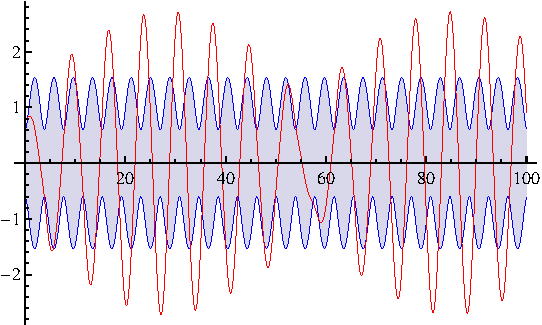
\includegraphics[width=0.65\textwidth]{Img/particle_core_envelope.pdf}
    \caption{束核包络与单粒子横向位移}
    \label{fig:particle_core_envelope}
\end{figure}

可以看出,束核的半径呈现规律的周期震荡。而当在每个周期的开始处对粒子的横向位置和动量进行观测时,我们可以得到一张粒子的庞加莱截面(Poincare surface of section),如图\ref{fig:particle_core_particle}所示,在粒子的庞加莱截面中可以看到明显的规律,粒子沿着某一条轨道进行运动。
\begin{figure}[!tbh]
    \centering
    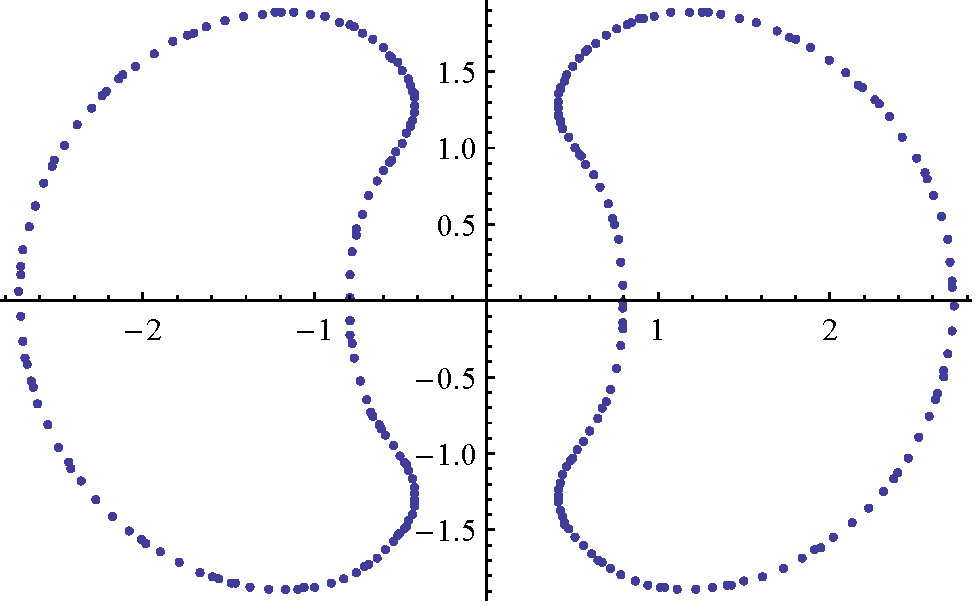
\includegraphics[width=0.65\textwidth]{Img/particle_core_particle.pdf}
    \caption{粒子的庞加莱截面}
    \label{fig:particle_core_particle}
\end{figure}

对粒子从中心到边界均匀排布,我们可以得到一组庞加莱截面,以显示不同初始位置处粒子的行为,如图\ref{fig:particle_core_Poincare}所示。四副图分别为不同的相位压缩因子$\eta$下的庞加莱截面,不同的颜色代表不同初始位置的粒子的轨迹。
\begin{figure}[!htbp]
  \centering
  ~%add desired spacing
  \begin{subfigure}[b]{0.6\textwidth}
    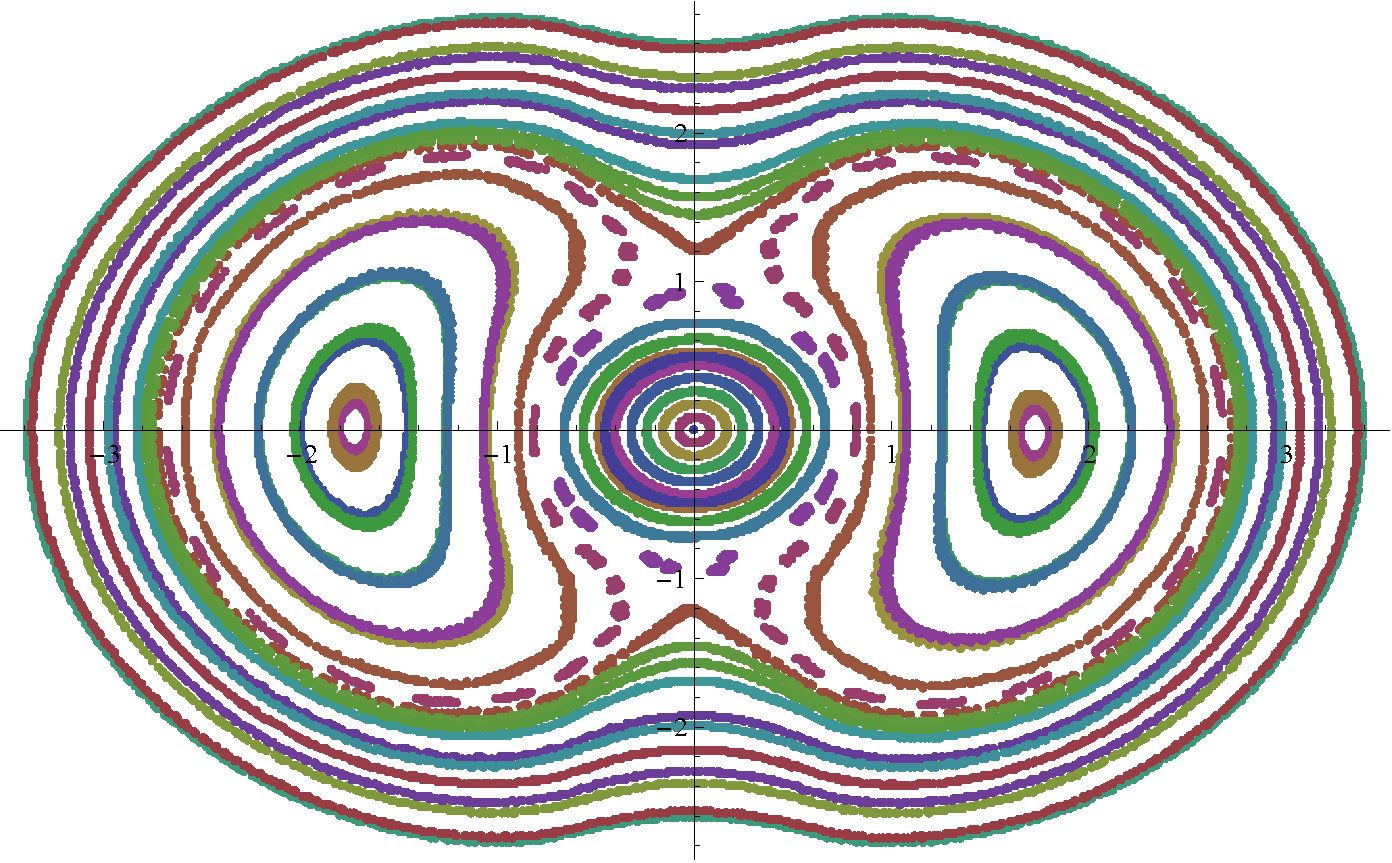
\includegraphics[width=\textwidth]{particle_core_Poincare5.pdf}
    \caption{$\eta = 0.5$}
    \label{fig:particle_core_Poincare5}
  \end{subfigure}
  ~
  \begin{subfigure}[b]{0.6\textwidth}
    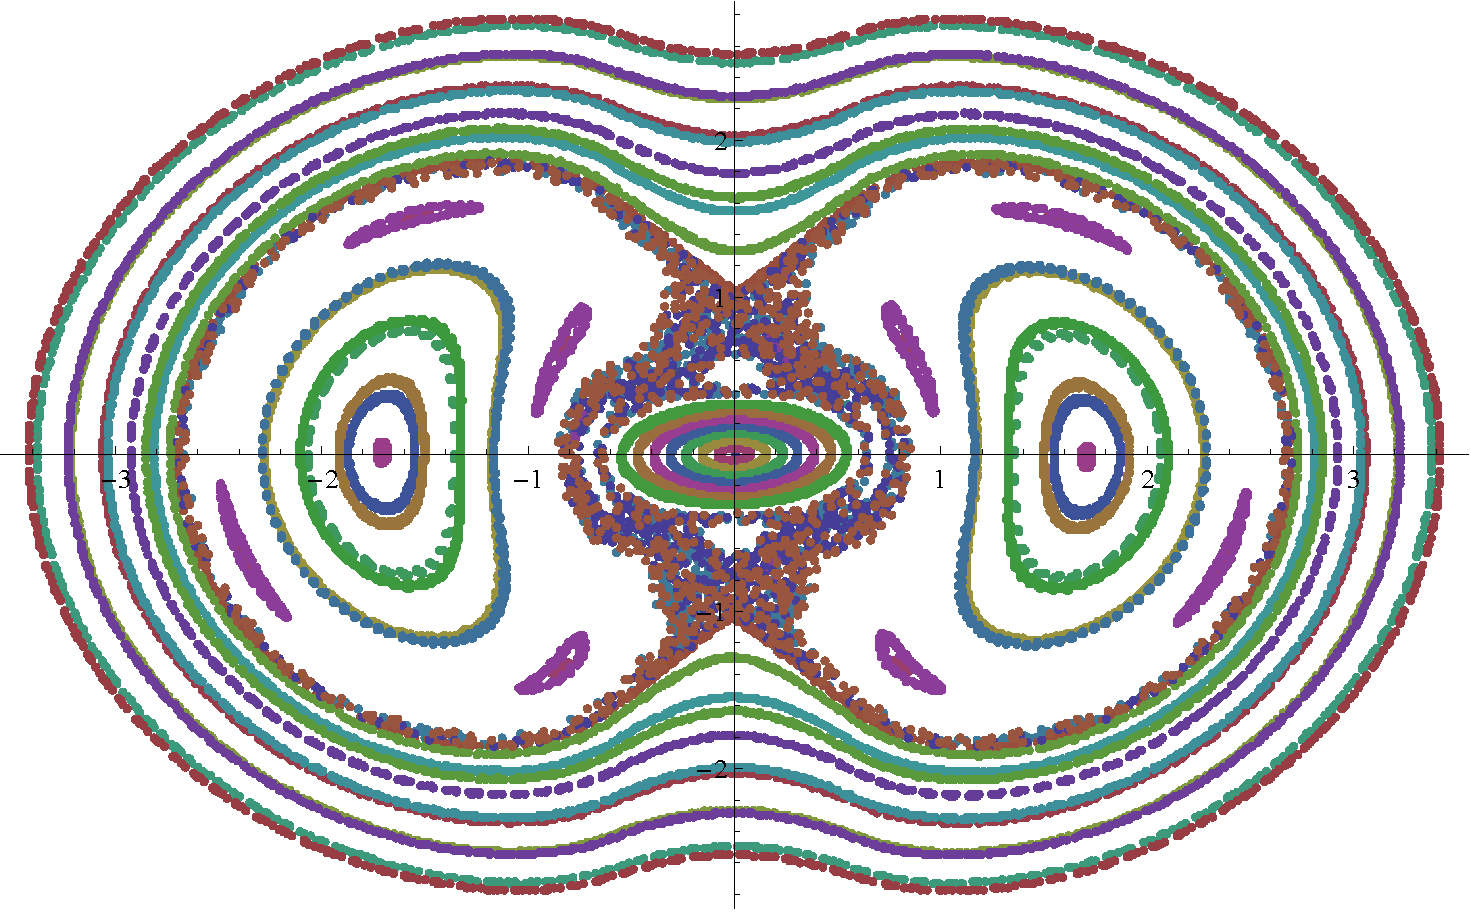
\includegraphics[width=\textwidth]{particle_core_Poincare3.pdf}
    \caption{$\eta = 0.3$}
    \label{fig:particle_core_Poincare3}
  \end{subfigure}%
  ~
  \begin{subfigure}[b]{0.6\textwidth}
    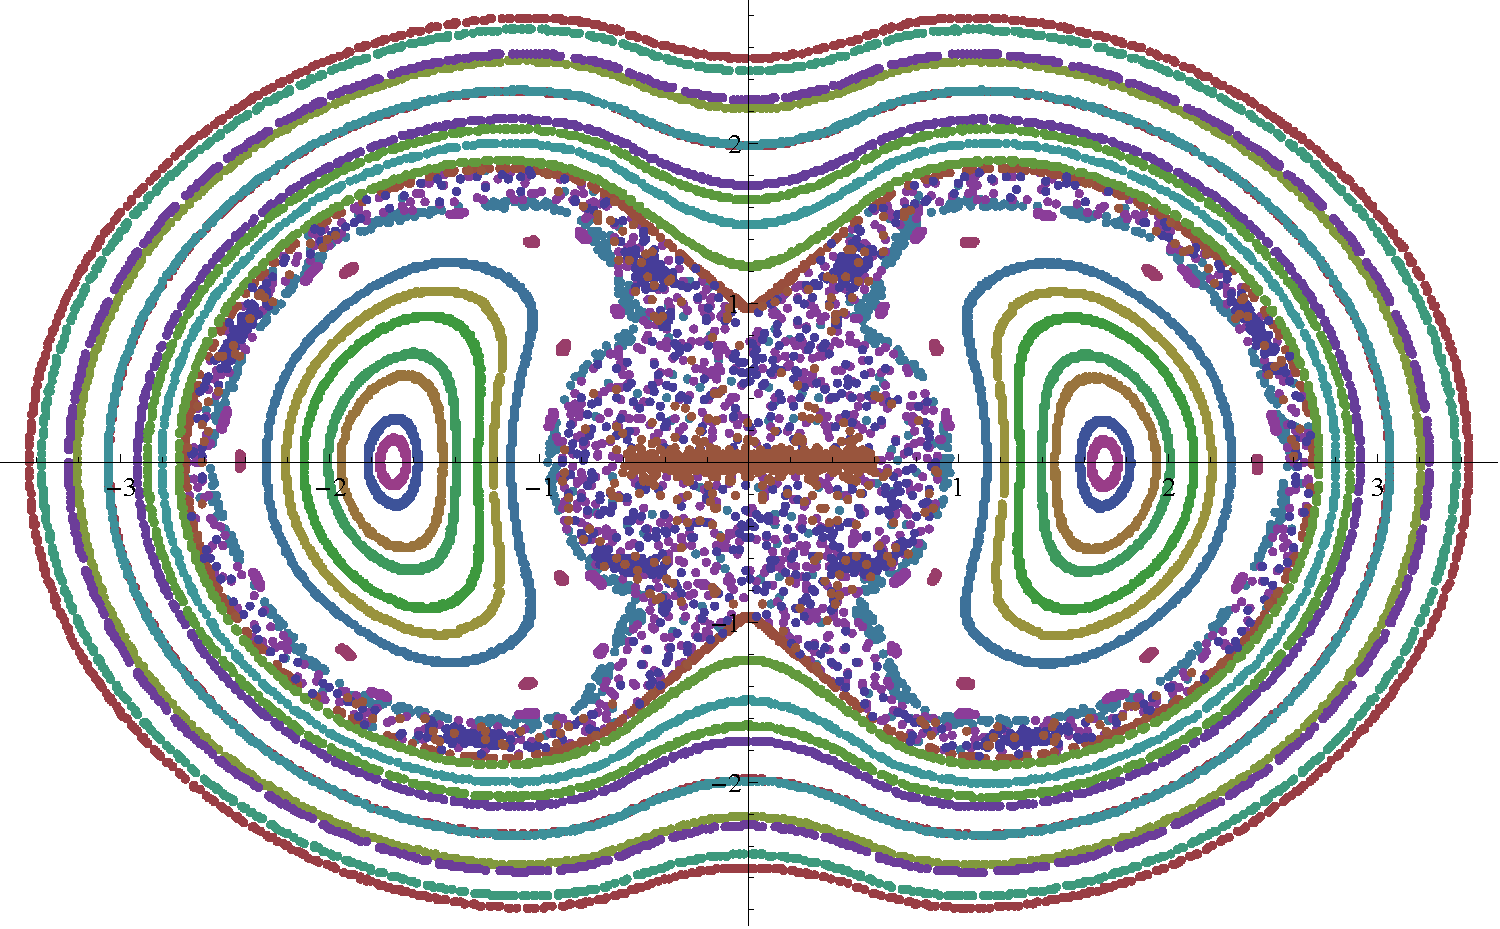
\includegraphics[width=\textwidth]{particle_core_Poincare1.pdf}
    \caption{$\eta = 0.1$}
    \label{fig:particle_core_Poincare1}
  \end{subfigure}%
  \caption{不同相位压缩因子下的庞加莱截面}
  \label{fig:particle_core_Poincare}
\end{figure}

庞加莱截面图可以分为三个区域:一,内椭圆区,大小约为束核半径及周边一小部分;二,不动点区,或者叫共振区,包括x轴上的不动点以及周围的环线,显示了参数共振的轨迹;三,外围类椭圆轨迹。
在空间电荷效应较弱的情况下,即$\eta$较大时,三个区的粒子都是做有规律的运动如图\ref{fig:particle_core_Poincare5}所示。但是当空间电荷主导的时候,比如$\eta=0.1$和$\eta=0.3$的时候(图\ref{fig:particle_core_Poincare3}和图\ref{fig:particle_core_Poincare1}),在内椭圆区会出现混沌行为,并且随着相位压缩因子变小,混沌行为变得更加明显,参数区的粒子轨迹也开始对初始条件敏感。

由庞加莱截面可以对束晕形成的机制进行分析,束晕中的粒子主要来源于共振区中的粒子,这些粒子最开始分布于内椭圆区与共振区的分界线附近,随着粒子运动,其向外移动到共振区与外椭园区的边界附近,在两个边界间震荡,形成了束晕。在空间电荷效应主导的情况下,内椭圆区的粒子也有可能形成束晕,如图\ref{fig:particle_core_Poincare1}所示,内椭圆区也出现了了混沌行为,最内部的粒子也会移动到外部形成束晕。

束核模型在一定程度上可以解释束晕形成的机制,但是这个模型并不是自洽的,与实际不相符。束核模型假设束核是稳定的,并且外部聚焦力是恒定的常数;而实际的束核有可能是不稳定的,外部的聚焦力也是可能变化的。因此,我们需要一个更加自洽的系统来研究束流的行为。

\section{束流模拟原理及PIC方法}   \label{section:PIC_algorithm}
数值模拟在束流动力学研究和加速器设计中非常重要,质点网格法(PIC方法)是一种使用自洽的系统对粒子进行模拟的算法。目前,主流的模拟软件都是使用的PIC求解空间电荷效应\cite{PIC_Birdsall1991, PIC_friedman1992, PIC_ji2000, PIC_ji2004, PIC_Amundson2006229, PIC_tracewin2014, PIC_beampath2005}。
使用PIC算法进行束流模拟的基本流程如图\ref{fig:PICflow1}和\ref{fig:PICflow2}所示。

\begin{figure}[!tbh]
%to be modified
  \centering
    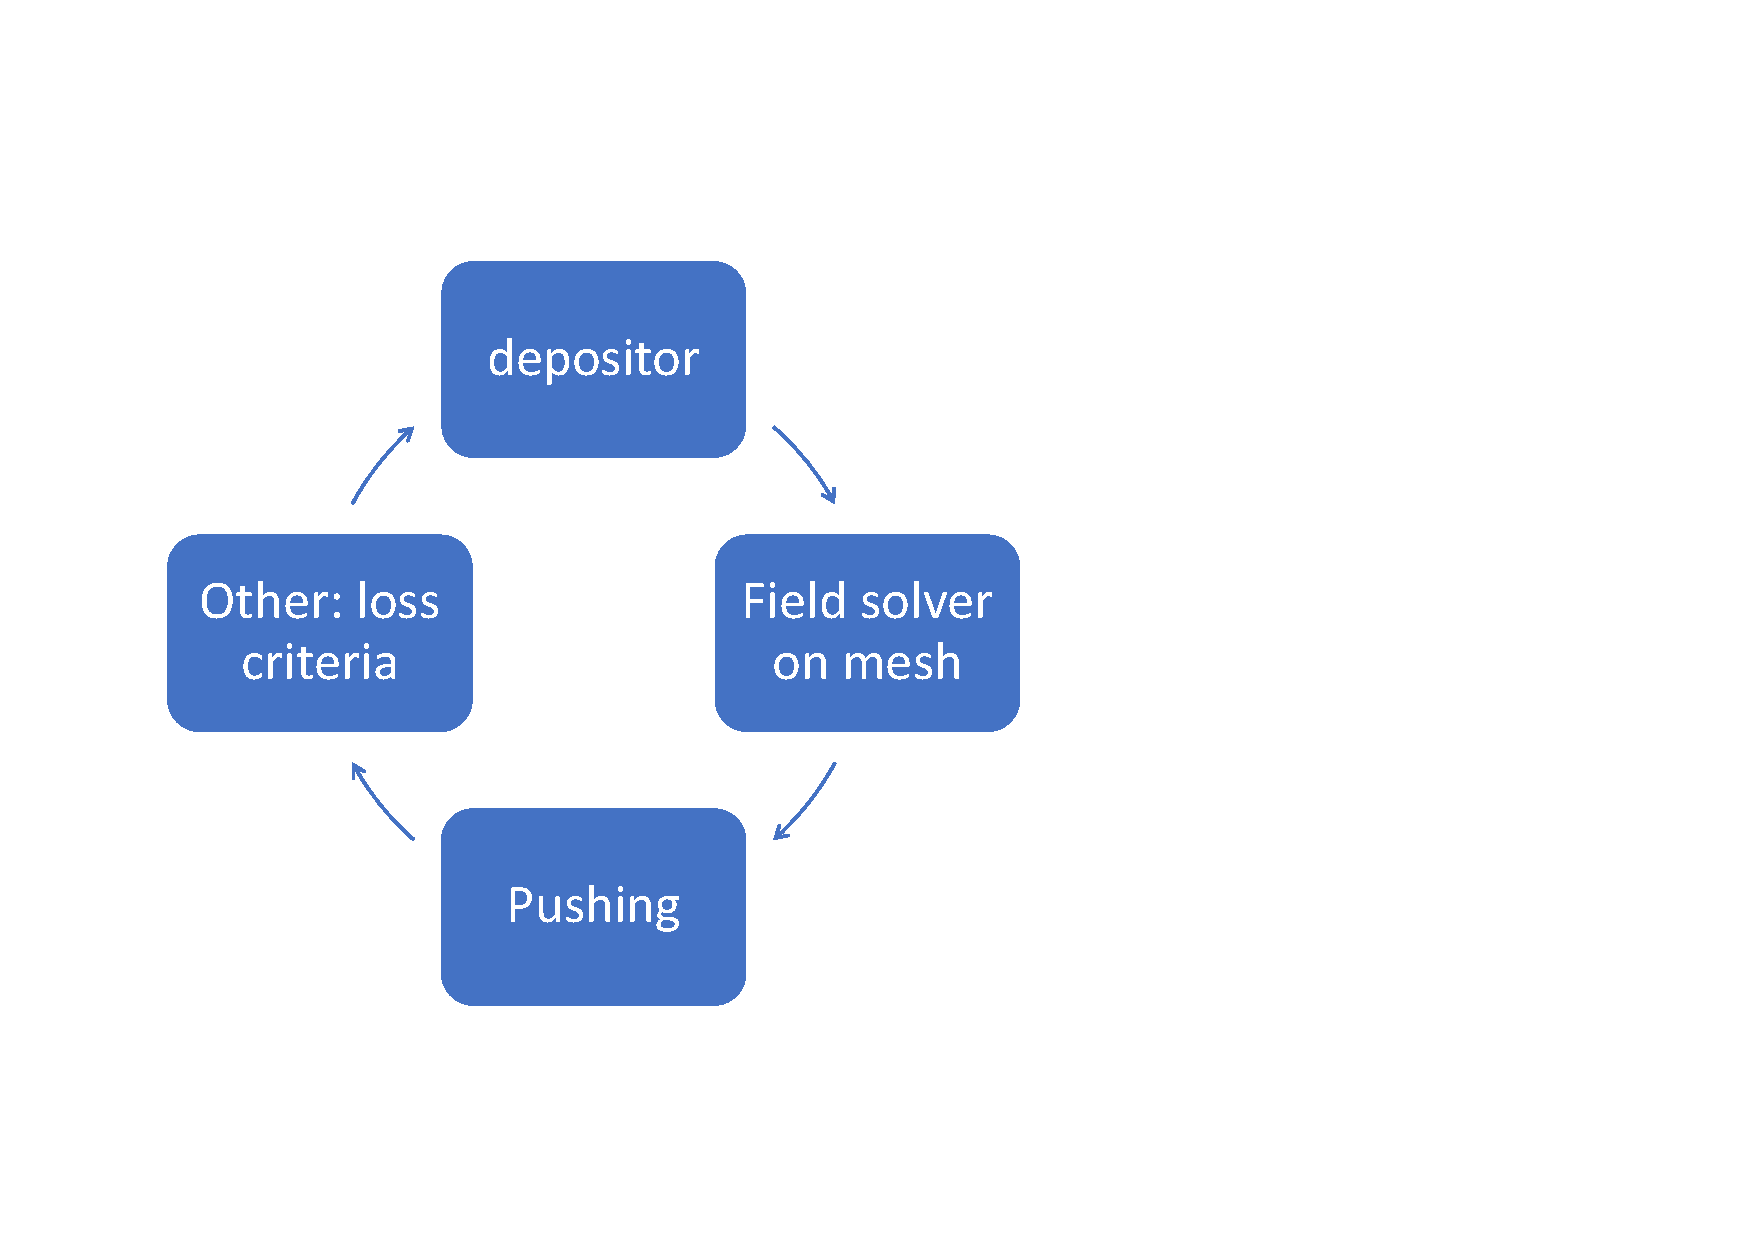
\includegraphics[width=0.6\textwidth]{Img/3_1_PIC.pdf}
    \caption{PIC算法块循环}
    \label{fig:PICflow1}
\end{figure}

\begin{figure}[!tbh]
  \centering
    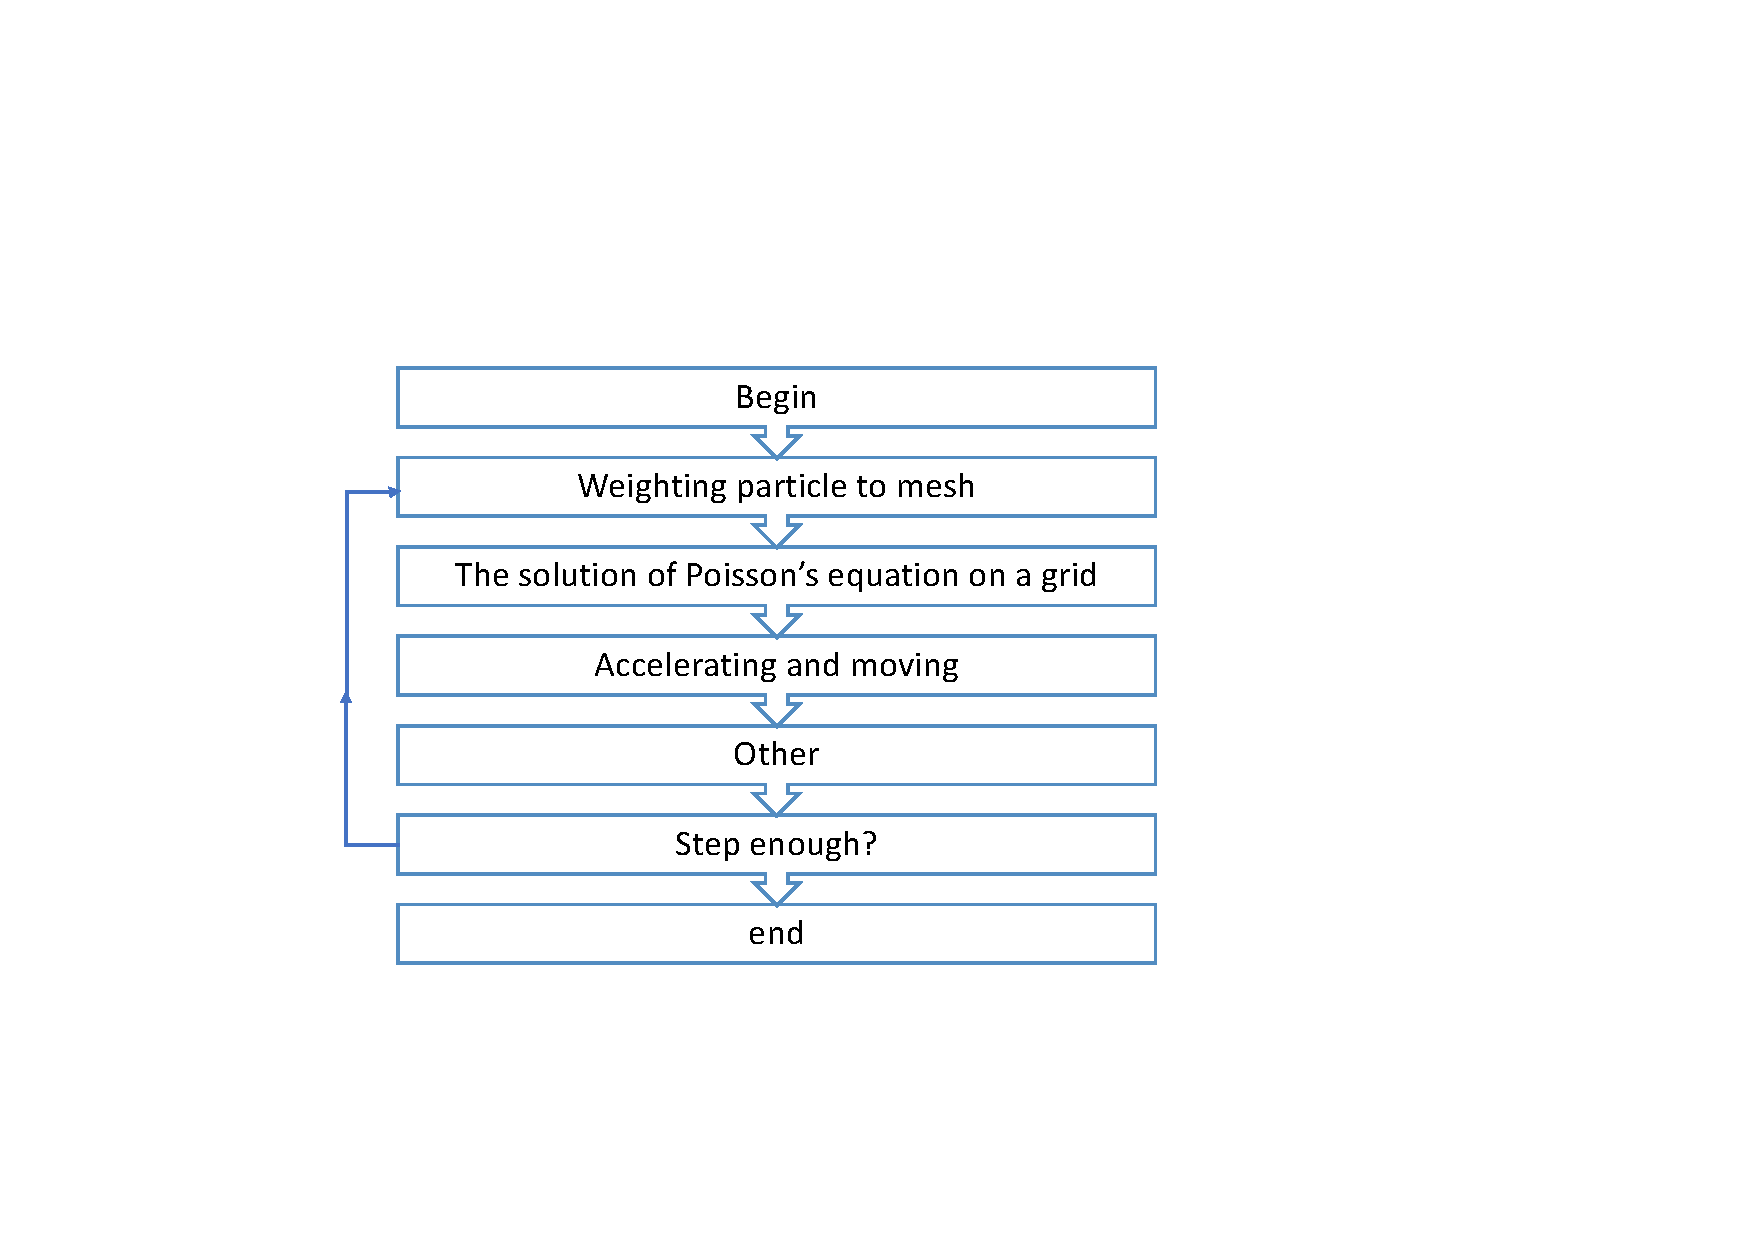
\includegraphics[width=0.7\textwidth]{Img/3_1_PIC2.pdf}
    \caption{PIC算法分段流程}
    \label{fig:PICflow2}
\end{figure}

首先,根据粒子的位置和范围确定所用的空间网格大小,然后执行以下循环:
\begin{enumerate}
  \item 将网格内的所有粒子的电荷根据粒子的位置分配到网格格点上,即从粒子分布得到获得空间点上的密度分布。
  \item 根据网格点上的电荷密度分布,求解网格点上的泊松方程,得到网格点上的电势分布。
  \item 根据电势分布,差分得到网格点上的电场分布。
  \item 根据粒子位置和网格上的电场分布,反向权重得到静止坐标系下粒子所受到的电场,再通过洛伦兹变换得到实验室坐标系下粒子所处位置的电磁场。
  \item 通过牛顿方程,推动粒子,更新粒子位置和动量。
\end{enumerate}

\subsection{权重差值}
PIC算法的第一步是将粒子电荷权重差值到网格上。
粒子权重差值主要有以下几个方面考虑:

\begin{enumerate}
  \item 如何将粒子电荷密度(3D)或者电流密度(2D)权重到空间网格上。
  \item 求解泊松方程后,如何将网格上的电场权重差值回粒子上。
  \item 如何确定网格点的数目和相对于粒子分布的位置及范围。
\end{enumerate}

其中,对于前两个问题,我们最好采用相同的差值算法的正反两个过程,来处理从粒子到网格和从网格到粒子的差值,从而避免算法上带来的非物理效应。如果采用不同的插值方法,可能会出现粒子自己推动自己的错误。

以一维问题为例,将粒子电荷权重到空间网格上的过程,可以理解为粒子坐标$x_i$到网格点上的电荷密度$\rho_p$的一个映射,其中$p$为网格点的坐标。一些常见的权重方法有最近网格点(Nearest Grid Point, NGP),网格云差分法({Cloud In Cell, CIC),三角云分配法(Triangular Shaped Cloud, TSC),如图\ref{fig:PIC_weighting}所示。图中,粒子处于$x$位置,而$p-1,p,p+1$代表不同的网格格点,不同颜色的面积大小代表分配给相应格点的电荷百分比。按照不同的形状分配可以得到不同的结果,
NGP方法为零阶差值,只将电荷分配到离粒子位置最近的网格点上,有较大误差。
CIC方法为一阶差值,根据粒子位置和格点位置的关系,如图\ref{fig:PIC_CIC}所示,将粒子按不同比例分配到临近的两个网格点上。
TSC方法为二阶差值,如图\ref{fig:PIC_TSC}所示,分配函数为三角形,将粒子按不同比例分配到临近的三个网格点上。
\begin{figure}[!htbp]
  \centering
  \begin{subfigure}[b]{0.8\textwidth}
    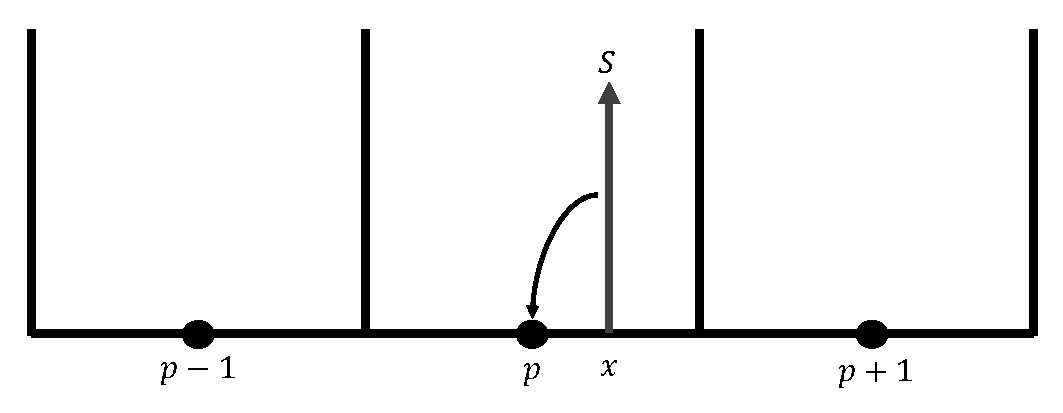
\includegraphics[width=\textwidth]{PIC_NGP}
    \caption{NGP}
    \label{fig:PIC_NGP}
  \end{subfigure}%
  ~%add desired spacing
  \begin{subfigure}[b]{0.8\textwidth}
    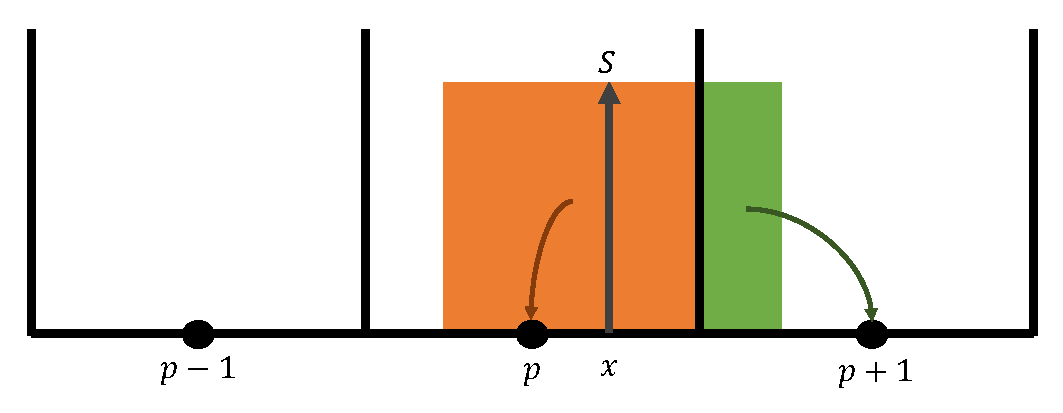
\includegraphics[width=\textwidth]{PIC_CIC}
    \caption{CIC}
    \label{fig:PIC_CIC}
  \end{subfigure}
  \begin{subfigure}[b]{0.8\textwidth}
    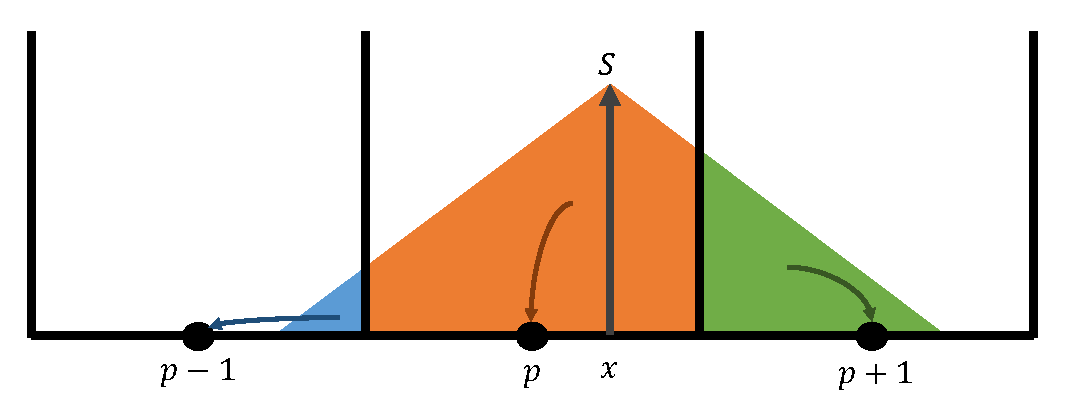
\includegraphics[width=\textwidth]{PIC_TSC}
    \caption{TSC}
    \label{fig:PIC_TSC}
  \end{subfigure}%
  \caption{分配方式示意图}
  \label{fig:PIC_weighting}
\end{figure}

在数学上,这个分配过程可以表示为:
\begin{equation}\label{eq:weight}
  \rho_p=\sum_{i}^{N_p} q_i W(x_i-x_p)
\end{equation}

其中,$q_p$为粒子电荷,$W(x)$为形状因子。如图\ref{fig:PIC_weighting2}所示,根据插值的阶数不同,$W(x)$有很多形式。下式给出了零阶,一阶,和而阶的形状因子:
\begin{equation}\label{eq:NGP}
  S_0(x)=\left\{
  \begin{aligned}
  &1, &\left| x \right| \leqslant \frac{\Delta x}{2} \\
  &0, &\left| x \right| >         \frac{\Delta x}{2}
  \end{aligned}
  \right.
\end{equation}
\begin{equation}\label{eq:CIC}
  S_1(x)=\left\{
  \begin{aligned}
  &1-\frac{\left| x \right|}{\Delta x}, &\left| x \right| \leqslant \Delta x \\
  &0                                  , &\left| x \right| >         \Delta x
  \end{aligned}
  \right.
\end{equation}
\begin{equation}\label{eq:TSC}
  S_2(x)=\left\{
  \begin{aligned}
  &\frac{1}{ \Delta x} \left[\frac{3}{4}-(\frac{\left| x \right|}{\Delta x})^2 \right], &\left| x \right| \leqslant \frac{\Delta x}{2} \qquad \quad \\
  &\frac{1}{2\Delta x} \left[\frac{3}{2}- \frac{\left| x \right|}{\Delta x}    \right], &\frac{\Delta x}{2} < \left| x \right| \leqslant \frac{3\Delta x}{2} \\
  &0,                                                                                   &\left| x \right| > \frac{3\Delta x}{2}\qquad \ \
  \end{aligned}
  \right.
\end{equation}


\begin{figure}[!htbp]
  \centering
  \begin{subfigure}[b]{0.8\textwidth}
    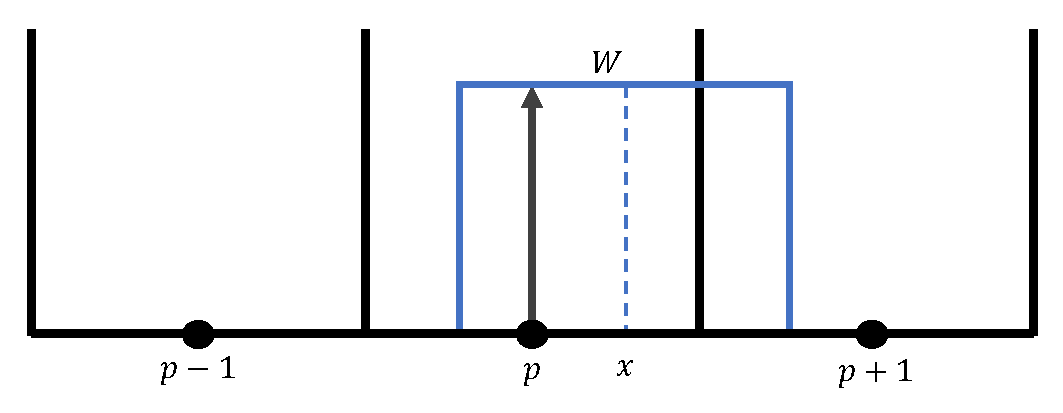
\includegraphics[width=\textwidth]{PIC_NGP2}
    \caption{NGP}
    \label{fig:PIC_NGP2}
  \end{subfigure}%
  ~%add desired spacing
  \begin{subfigure}[b]{0.8\textwidth}
    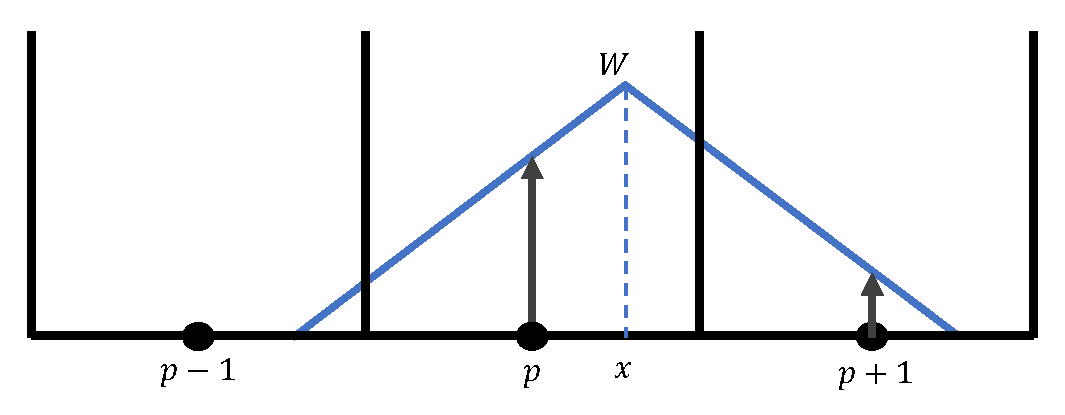
\includegraphics[width=\textwidth]{PIC_CIC2}
    \caption{CIC}
    \label{fig:PIC_CIC2}
  \end{subfigure}
  \begin{subfigure}[b]{0.8\textwidth}
    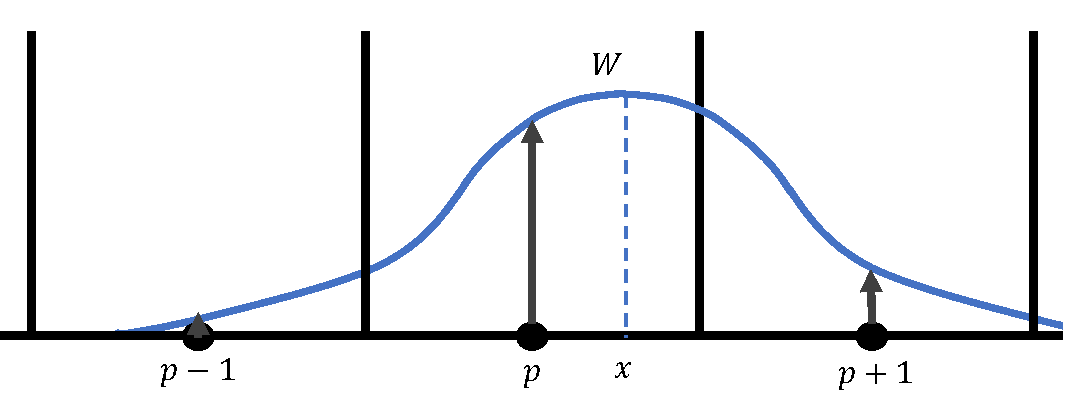
\includegraphics[width=\textwidth]{PIC_TSC2}
    \caption{TSC}
    \label{fig:PIC_TSC2}
  \end{subfigure}%
  \caption{形状因子方程}
  \label{fig:PIC_weighting2}
\end{figure}

在数值模拟中,低阶的算法,比如NGP,会带来很大的粒子离散误差。为了避免数值误差,我们需要采取高阶精度的算法,但是高阶的算法会导致计算量的增大,不满足计算的要求,所以实际中往往采用CIC差值方法。在P-TOPO中,所有的差值形式都采用一阶的线性差值(CIC)。

对于实际的三维问题,处理方法也是类似,我们采用立方网格,使用体积权重法来计算网格上的电荷。

\subsection{使用FFT解泊松方程}
\label{section:PIC_FFT}
经过由粒子到空间网格的权重插值后,我们得到了分布在网格点上的电荷密度分布函数。接下来要做的就是求解网格点上的泊松方程,对于本程序而言,我们使用快速傅里叶变换(FFT)的方法来求解。以一维问题为例,泊松方程:
\begin{equation}\label{eq:Poisson}
\nabla^2 \phi = -\frac{\rho}{\epsilon _0}
\end{equation}
在网格上可以离散表示为:
\begin{equation}\label{eq:PoissonGrid}
\frac{\phi_{j-1}-2\phi_{j}+\phi_{j}}{\Delta _{x}^{2}}=-\frac{\rho _j}{\epsilon _0}
\end{equation}
其中,$\phi_{j}$为第$j$个格点上的电势,$\rho_{j}$为第$j$个格点上的电荷量,$\Delta _{x}$为两个格点之间的距离。

将$\phi_{j}$和$\rho_{j}$进行傅里叶展开,我么可以得到:
\begin{align}
\label{eq:FFT@phi}
\phi _j &= \frac{1}{N_x} \sum_{n=0}^{N_x}{\phi_n \exp{(-\frac{i2 \pi n j}{N_x} )}} \\
\label{eq:FFT@rho}
\rho _j &= \frac{1}{N_x} \sum_{n=0}^{N_x}{\rho_n \exp{(-\frac{i2 \pi n j}{N_x} )}}
\end{align}
其中,$N_x$为一个方向上网格点的数目。

将式\ref{eq:FFT@phi}和式\ref{eq:FFT@rho}代回式\ref{eq:PoissonGrid}可得:
\begin{equation}\label{eq:FFT@PIC2}
\begin{aligned}
\sum_{n=0}^{N_x}{\phi_n
\left(\exp{(-\frac{i2 \pi n (j-1)}{N_x} )}  -2\exp{(-\frac{i2 \pi n j}{N_x} )}  +  \exp{(-\frac{i2 \pi n (j+1)}{N_x} )}\right)} \\
= \frac{\Delta _{x}^{2}}{\epsilon _0} \sum_{n=0}^{N_x}{\rho_n \exp{(-\frac{i2 \pi n j}{N_x} )}} \qquad\qquad\qquad
\end{aligned}
\end{equation}

对于傅里叶空间的的电势和电荷密度,我们可以得到$\phi_{n}$和$\rho_{n}$的关系:
\begin{equation}\label{eq:FFT@PIC3}
\phi_{n}\left(\exp{(\frac{i2 \pi n}{N_x} )}  +  \exp{(-\frac{i2 \pi n}{N_x})} - 2 \right)
 = \frac{\Delta _{x}^{2}}{\epsilon _0} {\rho_n} \\
\end{equation}
化简得到
\begin{equation}\label{eq:FFT@PIC3}
\phi_{n} = \frac{\rho_n}{\epsilon _0 K_n^2} \\
\end{equation}
其中
\begin{equation}\label{eq:FFT@PIC4}
K_n = (\frac{2\pi n}{N_x \Delta _x}) \frac{\sin({\pi n}/{N_x})}{{\pi n}/{N_x}} \\
\end{equation}

可以看出,通过傅里叶变换得到的傅里叶空间中的电荷密度$\rho_{n}$,我们可以得到傅里叶空间中的电势分布函数$\phi_{n}$。然后再经过傅里叶逆变换,我们就可以得到是空间中的电势分布$\phi_{j}$,最后经过差分我们就可以得到空间电场分布函数。如图\ref{fig:PIC_FFT_Poisson}所示:
\begin{figure}[ht]
  \begin{equation*}
    \centering
    \rho_j \quad \xrightarrow{FFT} \quad \rho_n  \quad \xrightarrow{Multuply\ by\ \frac{1}{K_n^2}}   \quad  \phi_n  \quad \xrightarrow{IFFT} \quad  \phi_j \quad \xrightarrow{Finite\ Difference} \quad  E_{x,j}
  \end{equation*}
  \caption{使用FFT求解泊松方程}
  \label{fig:PIC_FFT_Poisson}
\end{figure}

需要注意的是,这种$\exp$指数的傅里叶变换方式决定了我们使用的是周期性边界条件。如果我们想要第一类边界条件,我们需要采用$\sin$函数变换,其变换过程与FFT类似。
在本程序中,我们在横向采用第一类边界条件,用来模拟边界处的电势为0;而在纵向采用周期性边界条件,用以模拟连续束流。

\subsection{使用蛙跳法推动粒子}
在束流模拟中,一般使用蛙跳法来推动粒子。蛙跳法满足一致性、同时性、高准确性、高稳定性四个条件:

\subsubsection{一致性}
      一致性是指差分方程和微分方程的一致。任何数值算法都是使用有限大小的步长来模拟一个连续的过程。
      因此,我们我们应该在时间步长无线小的时候,使其效果与连续推动一致。
      
      考虑经典的牛顿方程:
      \begin{align}
        \label{eq:PIC_push1}
         \frac{\mathrm{d} \mathbf{x}}{\mathrm{d} t} &= \mathbf{v}  \\
        \label{eq:PIC_push2}
        m\frac{\mathrm{d} \mathbf{v}}{\mathrm{d} t} &= \mathbf{F}
      \end{align}
      如果我们采用有限步长$\Delta T$ 来推动粒子位置:
      \begin{align}
         \label{eq:PIC_push3}
         \frac{\mathbf{x}_{n+1}-\mathbf{x}_n}{\Delta T} &= \mathbf{v}_n  \\
         \label{eq:PIC_push4}
          m\frac{\mathbf{v}_{n+1}-\mathbf{v}_n}{\Delta T} &= \mathbf{F}_n
      \end{align}
      当其步长$\Delta T$足够小时,其结果应该与微分方程\ref{eq:PIC_push1} 和\ref{eq:PIC_push2}相一致。
\subsubsection{同时性}
      同时性又叫做可逆性。微分方程\ref{eq:PIC_push1}和\ref{eq:PIC_push2}是可逆的。例如,一个粒子在给定的力场中沿时间正向积分运动,然后如果将其速度取反,并沿时间反向积分,粒子将会沿着正向的轨迹向回运动,并能回到起始点。

      这一点在差分近似中并不能得到保证,比如,差分方程\ref{eq:PIC_push3}和\ref{eq:PIC_push4}中,粒子在第$n+1$步处取反,粒子位置变化为
      \begin{equation}
         \label{eq:PIC_push5}
         \frac{\mathbf{x}_{n}-\mathbf{x}_{n+1}}{\Delta T} = -\mathbf{v}_{n+1}
      \end{equation}
      其速度为$\mathbf{v}_{n+1}$而不是$\mathbf{v}_{n}$,也就是说粒子并不能沿其轨迹回到初始位置。这是因为差分方程的左右的时间中心不相同,式\ref{eq:PIC_push3}左侧,位置改变为$\mathbf{x}_{n+1}-\mathbf{x}_n$,是以$t_{n+1/2}$为时间中心的;而右侧$\mathbf{v}_n$是时间$t_{n}$ 时的速度。因此,我们需要将其改变为:
      \begin{align}
         \label{eq:PIC_push6}
         \frac{\mathbf{x}_{n+1}-\mathbf{x}_n}{\Delta T} &= \mathbf{v}_{n+1/2}  \\
         \label{eq:PIC_push7}
          m\frac{\mathbf{v}_{n+1/2}-\mathbf{v}_{n-1/2}}{\Delta T} &= \mathbf{F}_n
      \end{align}
      这也就是蛙跳法,即位置的时间与速度的时间并不在统一时刻,而是采用相差半个步长,然后交替推动粒子的速度和位置,以满足同时性条件。
\subsubsection{准确性}

      准确性与一步计算中的数值解与解析解的误差有关。这个误差主要来源于两方面:第一,来自于计算机的精度,例如,双精度浮点数仅有十四或十五位有效数字;第二,来自于使用有限小的步长代表连续变量的截断误差。通常来讲,第一种来自计算机数值精度的误差非常小,如果算法是稳定的(关于稳定性的论述见下一条),这个误差是可以忽略的。第二种来自于有限小的步长的误差,可以由解析解与数值解的差值来表示,其差值通常与步长$\Delta T$的$n$ 次方$(\Delta T)^n$的成正比,而不同算法之间的稳定性可由阶数$n$来表示。

      由式\ref{eq:PIC_push6}和\ref{eq:PIC_push7} 可知,蛙跳法为解析解\ref{eq:PIC_push1}和\ref{eq:PIC_push2}的二阶近似。证明如下:由式\ref{eq:PIC_push6} 和\ref{eq:PIC_push7}可得:
      \begin{equation}
         \label{eq:leapfrog_accuracy}
         \frac{\mathbf{x}_{n+1}-2\mathbf{x}_{n}+\mathbf{x}_{n-1}}{(\Delta T)^2} = \frac{\mathbf{F}(\mathbf{x}_n)}{m}
      \end{equation}
      如果$\mathbf{X}$为解析解:
      \begin{equation}
         \label{eq:leapfrog_accuracy2}
         \frac{\mathrm{d}^2 \mathbf{X}}{\mathrm{d} t^2} = \frac{\mathbf{F}}{m}
      \end{equation}
      那么有限小步长的误差可以由${\delta}^n$表示:
      \begin{equation}
         \label{eq:leapfrog_accuracy3}
         \frac{\mathbf{X}_{n+1}-2\mathbf{X}_{n}+\mathbf{X}_{n-1}}{(\Delta T)^2} = \frac{\mathbf{F}(\mathbf{X}_n)}{m} - {\delta}^n
      \end{equation}
      将$\mathbf{X}_{n+1}$和$\mathbf{X}_{n-1}$泰勒在$\mathbf{X}_{n}=\mathbf{X}(t_n)$ 处展开,式\ref{eq:leapfrog_accuracy3}可以写作:
      \begin{equation}
         \label{eq:leapfrog_accuracy4}
         \frac{\mathrm{d}^2 \mathbf{X}}{\mathrm{d} t^2} + \frac{(\Delta T)^2}{12} \frac{\mathrm{d}^4 \mathbf{X}}{\mathrm{d} t^4} + h.o.t. =  \frac{\mathbf{F}(\mathbf{X}_n)}{m} - {\delta}^n
      \end{equation}
      其中 $h.o.t.$ 为高阶项(high order term)。式\ref{eq:leapfrog_accuracy3} 与式\ref{eq:leapfrog_accuracy4}相减可得:
      \begin{equation}
         \label{eq:leapfrog_accuracy5}
         {\delta}^n = -\frac{(\Delta T)^2}{12} \frac{\mathrm{d}^4 \mathbf{X}}{\mathrm{d} t^4} + h.o.t.
      \end{equation}
      即,蛙跳法为二阶准确度(${\delta}^n \propto (\Delta T)^2$)。
\subsubsection{稳定性}
稳定性与误差随时间的变化有关。即使算法每一步的误差非常小,最终误差也有可能由于累积效应导致变大。
在一个数值算法中,如果每一步的误差不会导致一个更大的累积误差,那么这个算法是稳定的。

下面,我们讨论蛙跳法的稳定性。根据式\ref{eq:leapfrog_accuracy},如果我们给定$\mathbf{x}_0 = \mathbf{X}_0,\mathbf{x}_1 = \mathbf{X}_1$作为初始条件,不考虑误差的情况下,我们可以得到之后的一系列解$\mathbf{X}_2,\mathbf{X}_3,\mathbf{X}_4,...$,其中:
      \begin{align}
         \label{eq:leapfrog_stability1}
         \mathbf{X}_{2}-2\mathbf{X}_{1}+\mathbf{X}_{0} &= \frac{\mathbf{F}(\mathbf{X}_1)}{m} {(\Delta T)^2} \\
         \label{eq:leapfrog_stability2}
         \mathbf{X}_{3}-2\mathbf{X}_{2}+\mathbf{X}_{1} &= \frac{\mathbf{F}(\mathbf{X}_2)}{m} {(\Delta T)^2}
      \end{align}

然而,由于误差存在,我们无法得到微分方程中的精确解$\mathbf{X}_2,\mathbf{X}_3,\mathbf{X}_4,...$,而是会得到一系列含有误差近似解$\mathbf{x}_2,\mathbf{x}_3,\mathbf{x}_4,...$:
      \begin{align}
         \label{eq:leapfrog_stability3}
         \mathbf{x}_{2}-2\mathbf{X}_{1}+\mathbf{X}_{0} &= \frac{\mathbf{F}(\mathbf{X}_1)}{m} {(\Delta T)^2} \\
         \label{eq:leapfrog_stability4}
         \mathbf{x}_{3}-2\mathbf{x}_{2}+\mathbf{X}_{1} &= \frac{\mathbf{F}(\mathbf{X}_2)}{m} {(\Delta T)^2}
      \end{align}

如此,在第二步处的误差为:
      \begin{equation}
         \label{eq:leapfrog_stability5}
         {\epsilon}_2 = \mathbf{x}_2 -\mathbf{X}_2
      \end{equation}

在随后的每一步计算中,含有误差的近似结果都会被使用,我们需要知道的是${\epsilon}_2$是如何影响后续计算结果。由式\ref{eq:leapfrog_stability3}和式\ref{eq:leapfrog_stability4}可得:
      \begin{equation}
         \label{eq:leapfrog_stabilit6}
         (\mathbf{X}_{3}+{\epsilon}_3)-2(\mathbf{X}_{x}+{\epsilon}_2)+\mathbf{X}_{1} = \frac{\mathbf{F}(\mathbf{X}_2+{\epsilon}_2)}{m} {(\Delta T)^2}
      \end{equation}
与式\ref{eq:leapfrog_stability2}相比较,可得:
      \begin{equation}
         \label{eq:leapfrog_stabilit7}
         {\epsilon}_3-2{\epsilon}_2 = \left(\mathbf{F}(\mathbf{X}_2+{\epsilon}_2)  -\mathbf{F}(\mathbf{X}_2) \right)\frac{{(\Delta T)^2}}{m}
      \end{equation}
将上式右侧在$\mathbf{x}=\mathbf{X}^2$处进行泰勒展开:
      \begin{equation}
         \label{eq:leapfrog_stabilit8}
         {\epsilon}_3-2{\epsilon}_2 \approx {\epsilon}_2\left. \frac{\partial\mathbf{F}}{\partial\mathbf{x}}\right|_{\mathbf{x}=\mathbf{X}^2} \frac{{(\Delta T)^2}}{m}
      \end{equation}
类似可得:
      \begin{equation}
         \label{eq:leapfrog_stabilit9}
         {\epsilon}_4-2{\epsilon}_3+{\epsilon}_2 = {\epsilon}_3\left. \frac{\partial\mathbf{F}}{\partial\mathbf{x}}\right|_{\mathbf{x}=\mathbf{X}^3} \frac{{(\Delta T)^2}}{m}
      \end{equation}
则第n步的误差为:
      \begin{equation}
         \label{eq:leapfrog_stabilit10}
         {\epsilon}_{n+1}-2{\epsilon}_n+{\epsilon}_{n-1} = {\epsilon}_n \left. \frac{\partial\mathbf{F}}{\partial\mathbf{x}}\right|_{\mathbf{x}=\mathbf{X}^n} \frac{{(\Delta T)^2}}{m}
      \end{equation}
上式并不能得到一个准确的误差递进关系,除非${\partial\mathbf{F}}/{\partial\mathbf{x}}$为常量。由于我们的目标是判断算法是否稳定,而不是算法有多稳定,所以我们考虑最坏的情况,使用$-|{\partial\mathbf{F}}/{\partial\mathbf{x}}|_{max}$代替${\partial\mathbf{F}}/{\partial\mathbf{x}}$,其中的负号是因为我们假设所计算的问题是有限边界,而不是会延伸到无穷远。可得误差随时间的变化方程:
      \begin{align}
         \label{eq:leapfrog_stabilit11}
         {\epsilon}_{n+1}-2{\epsilon}_n+{\epsilon}_{n-1} &= -\left| \frac{\partial\mathbf{F}}{\partial\mathbf{x}}\right|_{max} \frac{{(\Delta T)^2}}{m} {\epsilon}_n \\
         {\epsilon}_{n+1}-2{\epsilon}_n+{\epsilon}_{n-1} &= -(\Omega \Delta T)^2 {\epsilon}_n
         \label{eq:leapfrog_stabilit12}
      \end{align}
其解的形式与震荡方程形式类似${\epsilon}_n = {\lambda}_n = \exp(i\omega n \Delta T)$。两个特征解${\lambda}_+$和${\lambda}_-$为:
      \begin{equation}
         \label{eq:leapfrog_stabilit13}
         {\lambda}_\pm = 1- \frac{(\Omega \Delta T)^2}{2}\pm \left[\frac{(\Omega \Delta T)^2}{2}\right]\left[1-\frac{4}{(\Omega \Delta T)^2}\right]^{1/2}
      \end{equation}
对于算法而言,想要保证数值上稳定,其误差不能随着时间而变大,即误差推动方程的特征解必须位于单位圆内,即$|\lambda|\leq1$。

因此,我们必须使时间步长足够小,才能保证算法稳定,对于蛙跳法而言,我们必须使:
      \begin{equation}
          \Omega \Delta T \leq 2
      \end{equation}
%\subsection{效率}
%blabla...


\section{Symplectic模型}          \label{section:symplectic_theory}
PIC算法是求解空间电荷效应非常快速有效的方法,在PIC算法中,粒子首先被根据位置权重到网格上,然后根据网格上的电荷密度求解泊松方程,得到网格上的电势,从而得到网格上的电场,再根据粒子位置反推出粒子所处位置的电场。使用这种方法,计算复杂度由直接的粒子-粒子方法的 $N_p^2$ 降低到了$\alpha N_p + \beta N_{cells}\log{N_{cells}}$。其中 $N_p$ 是粒子数,而$N_{cells}$ 是网格点数目。

然而,由于PIC算法不可避免的会带来网格热噪声,因此目前加速器界常用的PIC算法并不能保障辛条件(symplectic)。其计算就会被引入非物理效应,并对最终的强流束流物理的分析和讨论会带来一些干扰。因此,在需要长程模拟(比如环形加速器)的物理分析中,我们需要一种保辛的算法。

最初,保辛算法本身是为了保障哈密顿系统中的辛条件而被研究 \cite{symplectic_channel1990, symplectic_yoshida1990}。最近,无网格保辛模型被引入到加速器研究中作为空间电荷求解器 \cite{symplectic_ji2017}。
这种模型并不利用网格,而是利用高阶分解来求解空间电荷效应。
相比PIC算法,这种方法能够显著的降低由于网格数值噪声带来的发射度增长。
然而,虽然能够保证辛条件,这种算法也有缺陷,最显著的就是计算量要大得多。
无网格算法的计算复杂度为 $\alpha N_p * N_{modes}$ ,其中$N_{modes}$为分解的阶数,在通常模拟中我们一般使用$16 \times 16 \times 16$ 阶,在这种配置下花费的时间比PIC算法要高两到三个数量级。
所以我们必须提高这个算法的运行速度,以提高算法的实用性。
幸运的是,由于无网格算法很适合并行的特性,这种算法能够很好的被加速,并且有很好的可扩展性。
下面,我们简要介绍保辛算法的基本原理。

在束流动力学模拟中,当且仅当雅可比矩阵$M_i$满足以下条件时,传输矩阵$ m_i $才是保辛的\cite{accelerator2004lee, accelerator2013chao}:
\begin{equation}
M_{i}^{T}J{{M}_{i}}=J
\end{equation}
其中,$J$ 是如下 $6N\times6N$ 的矩阵:
\begin{equation}
J=\left(
  \begin{array}{cc}
     0 & I \\
    -I & 0 \\
  \end{array}
\right)
\end{equation}

对于考虑其空间电荷力的多粒子系统,哈密尔顿量可以写为:
\begin{equation}
H={{H}_{1}}+{{H}_{2}}
\end{equation}
其中
\begin{eqnarray}
% \nonumber to remove numbering (before each equation)
  {H}_{1} &=& \sum\limits_{i}{{p_{i}^{2}}/{2}\;}+\sum\limits_{i}{q\psi ({{r}_{i}})} \\
  {H}_{2} &=& \frac{1}{2}\sum\limits_{i}{\sum\limits_{j}{q\varphi ({{r}_{i}},{{r}_{j}})}}
\end{eqnarray}

其中${{H}_{1}}$ 只包含外场信息,而 ${{H}_{2}}$ 只包括空间电荷效应。根据${{H}_{1}}$ 和 ${{H}_{2}}$ 得到的两个传输矩阵 ${{m}_{1}}$和 ${{m}_{2}}$,一个二阶传输矩阵$m\left( \tau  \right)$可以被定义为:
\begin{equation}
m\left( \tau  \right)={{m}_{1}}\left( \tau /2 \right){{m}_{2}}\left( \tau  \right){{m}_{1}}\left( \tau /2 \right)
\end{equation}

如果$ {{m} _ {1}} $和$ {{m} _ {2}} $都是保辛的,那么$ m $就是保辛的。在大多数加速器元件中,我们可以通过单粒子动力学获得相应的外场传输矩阵$ {{m} _ {1}} $,而内场传输矩阵$ {{m} _ {2}} $可以写为:
\begin{eqnarray}
 {{r}_{i}}(\tau ) &=& {{r}_{i}}(0) \\
 {{p}_{i}}(\tau ) &=& {{p}_{i}}(0)-\frac{\partial {{H}_{2}}(r)}{\partial {{r}_{i}}}\tau
\end{eqnarray}
其雅克比矩阵为:
\begin{equation}
{{M}_{2}}=\left(
\begin{array}{cc}
   I & 0  \\
   L & I  \\
\end{array} \right)
\end{equation}
其中
${{L}_{ij}}=\frac{\partial {{p}_{i}}(\tau )}{\partial {{r}_{j}}}=-\frac{{{\partial }^{2}}{{H}_{2}}(r)}{\partial {{r}_{i}}\partial {{r}_{j}}}\tau$
是一个对称矩阵,所以${{M}_{2}}$满足保辛条件.

对于一个3D束团, ${{H}_{2}}$可以表示为:
\begin{equation}
{{H}_{2}}=\kappa {{\gamma }_{0}}\sum\limits_{i}{\sum\limits_{j}{\varphi ({{r}_{i}},{{r}_{j}})}}
\end{equation}
其中 $\kappa =q/(lm{{C}^{2}}\gamma _{0}^{2}{{\beta }_{0}}),l=C/\omega $。而在束流坐标系下的静电势可以有泊松方程得到:
\begin{equation}
\frac{{{\partial }^{2}}\phi }{\partial {{x}^{2}}}+\frac{{{\partial }^{2}}\phi }{\partial {{y}^{2}}}+\frac{{{\partial }^{2}}\phi }{\partial {{z}^{2}}}=-\frac{\rho }{{{\varepsilon }_{0}}}
\end{equation}
其中边界条件为:
\begin{equation}
\begin{array}{cc}
   \phi (x=0,y,z)=0, & \phi (x=a,y,z)=0  \\
   \phi (x,y=0,z)=0, & \phi (x,y=b,z)=0  \\
   \phi (x,y,z=0)=0, & \phi (x,y,z=c)=0  \\
\end{array}
\end{equation}
其中,$a$,$b$,$c$分别是X,Y,Z方向上的零电势边界长度。如果我们将$c$设的足够大,电势将在无穷远处为零。

泊松方程中的电势$\phi$和电荷密度$\rho$可以展开为:
\begin{eqnarray}
 \rho(x,y,z)&=&\sum\limits_{l=1}^{{{N}_{l}}}{\sum\limits_{m=1}^{{{N}_{m}}}{\sum\limits_{n=1}^{{{N}_{n}}}{{{\rho }^{lmn}}\sin ({{\alpha }_{l}}x)\sin ({{\beta }_{m}}y)\sin ({{\gamma }_{n}}z)}}} \\
 \phi(x,y,z)&=&\sum\limits_{l=1}^{{{N}_{l}}}{\sum\limits_{m=1}^{{{N}_{m}}}{\sum\limits_{n=1}^{{{N}_{n}}}{{{\phi }^{lmn}}\sin ({{\alpha }_{l}}x)\sin ({{\beta }_{m}}y)\sin ({{\gamma }_{n}}z)}}}
\end{eqnarray}
其中 ${N}_{l}$,${N}_{m}$,${N}_{n}$分别为电势和电荷密度在X,Y,Z三个方向上展开的阶数,而 ${\rho }^{lmn}$和 ${\phi }^{lmn}$可以表达为:
\begin{eqnarray}
  {{\rho }^{lmn}}&=&\frac{8}{abc}\int\limits_{0}^{a}{\int\limits_{0}^{b}{\int\limits_{0}^{b}{\rho (x,y,z)\sin ({{\alpha }_{l}}x)\sin ({{\beta }_{m}}y)\sin ({{\gamma }_{n}}z)dxdydz}}} \\
 {{\phi }^{lmn}}&=&\frac{8}{abc}\int\limits_{0}^{a}{\int\limits_{0}^{b}{\int\limits_{0}^{b}{\phi (x,y,z)\sin ({{\alpha }_{l}}x)\sin ({{\beta }_{m}}y)\sin ({{\gamma }_{n}}z)dxdydz}}}
\end{eqnarray}
其中
\begin{equation}
{{\alpha }_{l}}=\frac{l\pi }{a},{{\beta }_{m}}=\frac{m\pi }{b},{{\gamma }_{n}}=\frac{n\pi }{c}
\end{equation}

将上面的展开代入泊松方程,我们可以得到:
\begin{equation}
{{\phi }^{lmn}}=\frac{{{\rho }^{lmn}}}{{{\varepsilon }_{0}}(\alpha _{l}^{2}+\beta _{m}^{2}+\gamma _{n}^{2})}
\end{equation}

据此,我们得到了粒子密度$ \ rho $和电势$ \ phi $之间的关系:
\begin{multline}
\phi (x,y,z)=\frac{1}{{{\varepsilon }_{0}}}\frac{8}{abc}\omega \times \\ \sum\limits_{j=1}^{{{N}_{j}}}{\sum\limits_{l=1}^{{{N}_{l}}}{\sum\limits_{m=1}^{{{N}_{m}}}{\sum\limits_{n=1}^{{{N}_{n}}}{\frac{\sin ({{\alpha }_{l}}{{x}_{j}})\sin ({{\beta }_{m}}{{y}_{j}})\sin ({{\gamma }_{n}}{{z}_{j}})\sin ({{\alpha }_{l}}x)\sin ({{\beta }_{m}}y)\sin ({{\gamma }_{n}}z)}{(\alpha _{l}^{2}+\beta _{m}^{2}+\gamma _{n}^{2})}}}}}
\end{multline}
其中 $\omega $ 是粒子的电荷。

于是哈密顿量 ${{H}_{2}}$可以表示为:
\begin{multline}
{{H}_{2}}=\frac{1}{{{\varepsilon }_{0}}}\frac{8}{abc}\omega \kappa {{\gamma}_{0}} \times \\
\sum\limits_{i=1}^{{{N}_{i}}}{\sum\limits_{j=1}^{{{N}_{j}}}{\sum\limits_{l=1}^{{{N}_{l}}}{\sum\limits_{m=1}^{{{N}_{m}}}{\sum\limits_{n=1}^{{{N}_{n}}}
{\frac{\sin ({{\alpha }_{l}}{{x}_{j}})\sin ({{\beta }_{m}}{{y}_{j}})\sin ({{\gamma }_{n}}{{z}_{j}})\sin ({{\alpha }_{l}}{{x}_{i}})\sin ({{\beta }_{m}}{{y}_{i}})\sin ({{\gamma }_{n}}{{z}_{i}})}{(\alpha _{l}^{2}+\beta _{m}^{2}+\gamma _{n}^{2})}}
}}}}
\end{multline}

我们得到了保辛的空间电荷传输矩阵 ${{m}_{2}}$。 以X方向为例:
\begin{align}
&{{x}_{i}}(\tau )= {{x}_{i}}(0) \\
 \nonumber &{{p}_{xi}}(\tau )= {{p}_{xi}}(0)-\tau \frac{1}{{{\varepsilon }_{0}}}\frac{8}{abc}\omega \kappa {{\gamma }_{0}} \times \\
 &\sum\limits_{j=1}^{{{N}_{j}}}{\sum\limits_{l=1}^{{{N}_{l}}}{\sum\limits_{m=1}^{{{N}_{m}}}{\sum\limits_{n=1}^{{{N}_{n}}}{\frac{{{\alpha }_{l}}\sin ({{\alpha }_{l}}{{x}_{j}})\sin ({{\beta }_{m}}{{y}_{j}})\sin ({{\gamma }_{n}}{{z}_{j}})\cos ({{\alpha }_{l}}{{x}_{i}})\sin ({{\beta }_{m}}{{y}_{i}})\sin ({{\gamma }_{n}}{{z}_{i}})}{(\alpha _{l}^{2}+\beta _{m}^{2}+\gamma _{n}^{2})}}}}}\label{eq:map1}
\end{align}
在Y和Z方向的传输矩阵与之类似。


\section{GPU和CPU架构}            \label{section:GPU_CPU}
GPU英文全称Graphic Processing Unit,中文为“图形处理器”。
GPU一开始是由于在现代的计算机中图形的处理变得越来越重要,需要一个专门的图形的核心处理器,使显卡减少对CPU的依赖,并进行部分原本CPU的工作;CPU是英文全称为Central Processing Unit,中文为“中央处理器”,一般由逻辑运算单元、控制单元和存储单元组成。
近年来,GPU高速发展,极大的提高了计算机图形处理的速度和质量,不但促进了图像处理、虚拟现实、计算机仿真等相关应用领域的快速发展,同时也为人们利用GPU进行图形处理以外的通用计算提供了良好的运行平台。

相对于CPU,GPU在并行处理和计算密集型问题方面具有很大优势。目前,GPU已成为普通计算机强大、高效的计算资源。如图\ref{fig:GPU}所示,一个CPU一般只拥有少数几个核,而一个GPU会有几百甚至几千个核。从系统架构上看,GPU针对向量计算进行了高度并行的数据流优化处理,这种多核架构特别适合进行数据并行。这种以数据流作为处理单元的机制,在对数据流的处理上可以取得很高的速度。
GPU 加速计算是指同时利用GPU 和 CPU,加快应用程序的运行速度\cite{gpu2008}。GPU厂商为科学计算设计了自己的API,其中CUDA(Compute Unified Device Architecture)就是NVIDIA设计的并行计算平台和编程规范\cite{nvidia2010programming}。利用CUDA,我们能够有效的利用GPU,使程序的运行效率大大提高。

根据使用CUDA的测试结果显示,利用GPU实现FFT(Fast Fourier Transformation)、BLAS(Basic Linear Algebra Subprograms)、排序及线性方程组求解等科学计算,与单纯依靠CPU实现的算法相比,平均性能提高了近20倍。
\begin{figure}[!htb]
    \centering
    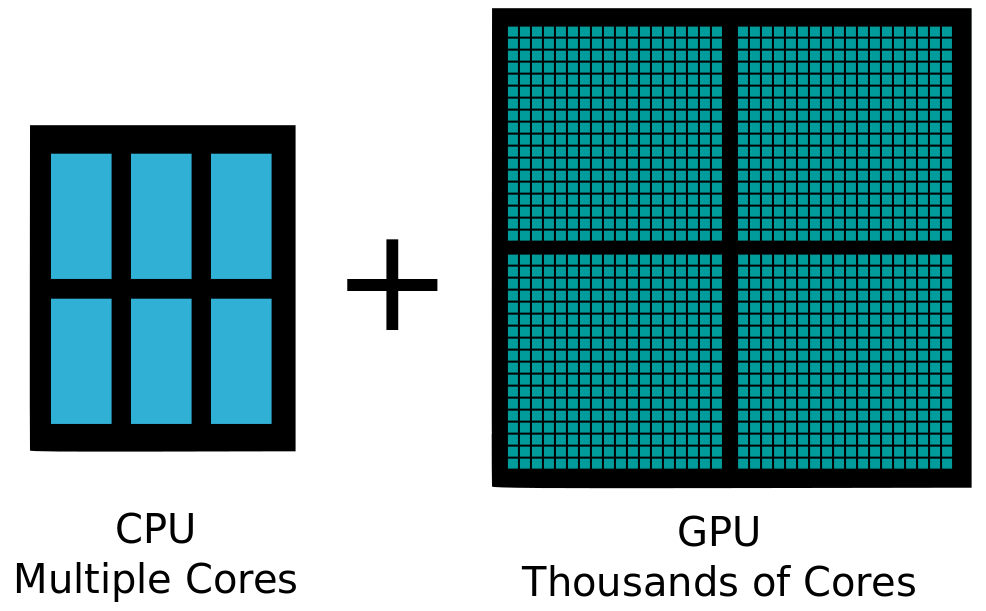
\includegraphics[width=0.9\textwidth]{plot/GPU_vs_CPU.png}
    \caption{GPU与CPU的结构对比}
    \label{fig:GPU}
\end{figure}

随着GPU可编程能力、并行处理能力和应用范围方面得到不断提升和扩展,GPU已成为当前计算机系统中性能很高的部件。
因此,我们对PIC算法和Symplectic算法都进行了GPU实现,充分利用了现有计算资源,发挥GPU的高性能计算能力,使程序在GPU与CPU之间进行协作,以提高模拟程序的运行效率。

\section{小结}                    \label{section:Algorithm_conclusion}
在本章中,介绍计算了几种求解空间电荷效应的模型及计算机并行的并行。
早期的束核模型存在稳定束核假设和对空间电荷力进行了线性近似,是一个非自洽模型。
只能在一定程度上定性解释束晕形成的机制,而无法定量的求解出实际加速器中的空间电荷效应的影响。

在束流模拟中,我们一般采用PIC算法来求解空间电荷力,使用蛙跳法推动粒子,其满足一致性、同时性、高准确性、高稳定性四个条件。
PIC算法是一个更加自洽的用来研究考虑空间电荷效应的束流行为的方法。
在PIC算法中,粒子首先被根据位置权重到网格上,
然后在网格上的求解泊松方程,以得到网格上的电势,
再根据粒子位置反推出粒子所处位置的电场。
PIC有效地降低了计算量,成为了国际上主流的空间电荷效应算法。

然而,由于PIC算法含有网格热噪声,会被引入一些非物理效应,我们引出了Symplectic模型。
这种模型利用对粒子的高阶分解来求解空间电荷效应。
相比PIC算法,Symplectic模型计算量要大得多,但是能够显著的降低PIC算法中由于网格热噪声带来的发射度增长。

由于Symplectic算法计算量巨大,PIC算法也有提高效率的需求,我们研究对比了不同的计算机并行处理器。
相比于CPU,GPU在逻辑判断上运算能力相对较弱,但是在并行计算密集型问题方面具有很大优势。
因此,我们在GPU上对PIC算法和Symplectic算法进行了实现,并且在CPU集群上对PIC算法进行了实现。




\chapter{模拟程序设计及算法实现}
\label{chap:Code}
随着加速器的流强越来越高,束流模拟代码在束流动力学研究中的作用也越来越重要,
尤其是在例如C-ADS,SNS,ESS等加速器中\cite{li2013physics,henderson2014spallation,eshraqi2016ess},
其非线性空间电荷效应占据主导地位。
一个拥有更强大的计算能力以及更高的精确度的程序,是我们研究强流束流动力学所必须的。

根据前一章中介绍的物理模型,在本章中我们对模拟程序的架构设计、代码实现、以及并行化优化策略进行介绍。
我们首先介绍P-TOPO程序的整体结构,之后分别介绍了PIC算法在GPU上和CPU集群上的的实现,和Symplectic在GPU上的实现。

\section{P-TOPO程序结构}
我们开发了一个新的粒子模拟程序,命名为Parallel-Trace of Particle Orbits (P-TOPO),致力于研究强流加速器中的空间电荷效应问题\cite{li2016nonlinear,li2014envelope,li16collective,li2015space}。
P-TOPO使用C++语言开发,并且使用OpenMP进行并行化,目标是在普通多核PC机上快速模拟粒子在加速器中的行为。
P-TOPO使用时间t,而不是使用位置z,作为基本的独立变量,这是研究粒子的空间电荷效应非常自然的选择。即时使用位置z作为基本变量,在求解空间电荷力的过程中,也需要将粒子坐标转换为同一时间t下的时空间坐标。
在P-TOPO中,产生外场的一些加速器元件,例如各种磁铁,螺线管,RFQ,的外场使用元件的解析模型得到;而对于另外一些元件,例如超导腔,我们首先读取场文件\cite{studio2008cst},然后采用二阶插值的方法获取粒子所受到的场的大小和方向。

对于束团内部的空间电荷效应,我们使用经典的PIC方法进行求解\cite{hockney1988computer}。PIC方法是研究空间电荷效应非常常用的的一种数值模拟算法\cite{PIC_birdsall2004plasma,PIC_luccio2002space}。PIC发展于上世纪七十年代,被广泛的应用于等离子体模拟和加速器设计。

P-TOPO的程序的结构如图\ref{fig:P_TOPO}所示,图中每一个条目为一个类:
\begin{itemize}
  \item 主类MAIN调用其他各个具体的类,比如从外部Lattice结构中获取外场,求解内部空间电荷力,以及根据粒子所受的场推动粒子的位置和动量。
  \item Lattice类根据外部输入文件,解析或者数值地构建加速器的结构,以及根据粒子坐标,给出粒子所受的外场力。
  \item Distribution类产生粒子的初始分布,目前可以产生 KV,Waterbag,Parabolic,和Gaussian四种粒子分布,如图\ref{fig:distribution}所示。
  \item Beam类统计粒子的信息,并且计算出如rms大小,发射度等束团参数,将其保存以供进一步分析和输出。
  \item Internal Field类通过PIC方法计算空间电荷效应,在PIC方法中,我们使用FFT 来求解Poisson方程。
  \item Leapfrog类和Runge-Kutta 4类都是继承Pusher类,是不同的推动粒子位置和动量的方法。
\end{itemize}

\begin{figure}[!htb]
    \centering
    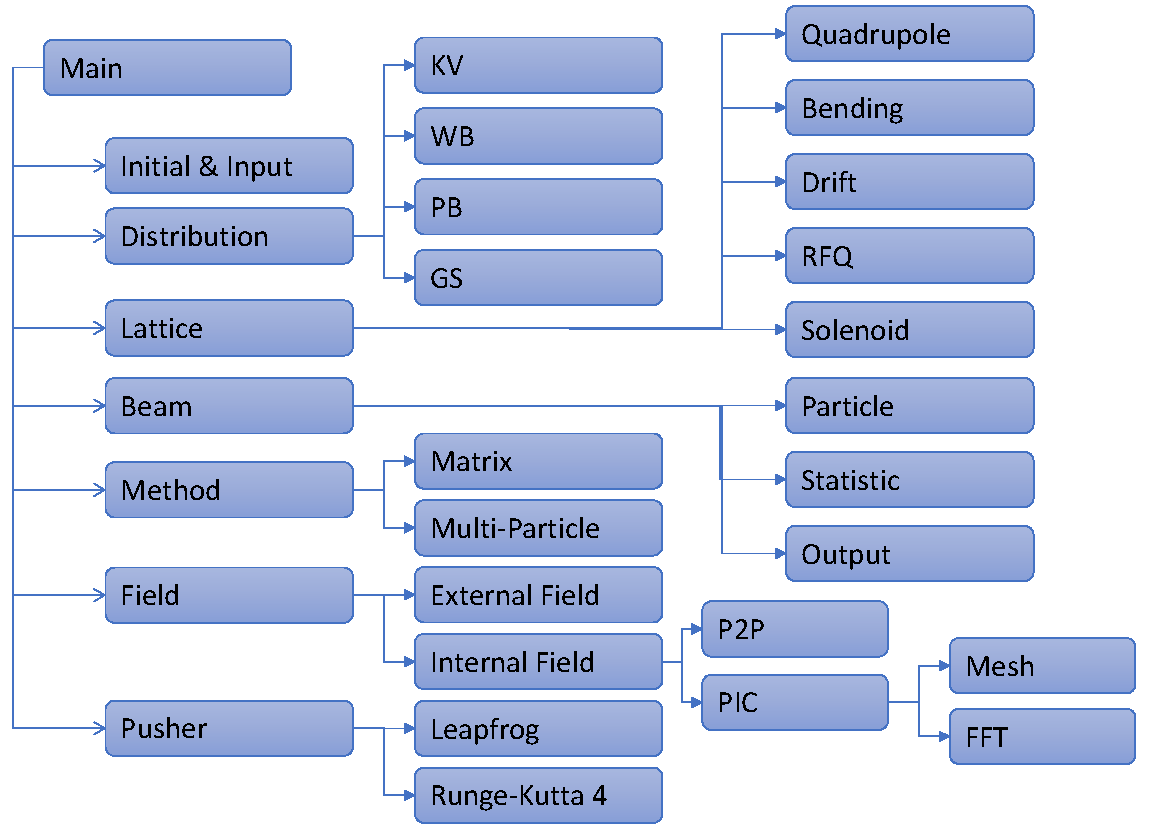
\includegraphics[width=0.8\textwidth]{Img/P_TOPO.pdf}
    \caption{P-TOPO程序结构}
    \label{fig:P_TOPO}
\end{figure}

\begin{figure}[!htb]
    \centering
    \begin{subfigure}[b]{0.48\textwidth}
        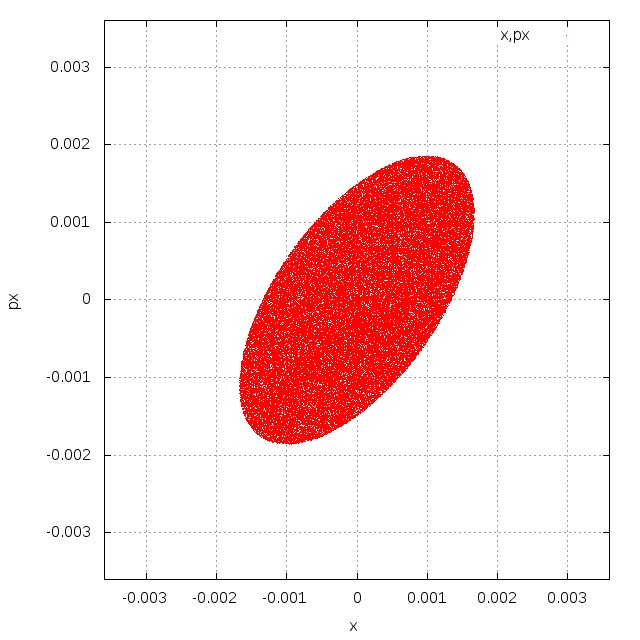
\includegraphics[width=\textwidth]{Img/KV_x_dx.jpg}
        \caption{KV}
    \end{subfigure}
    \begin{subfigure}[b]{0.48\textwidth}
        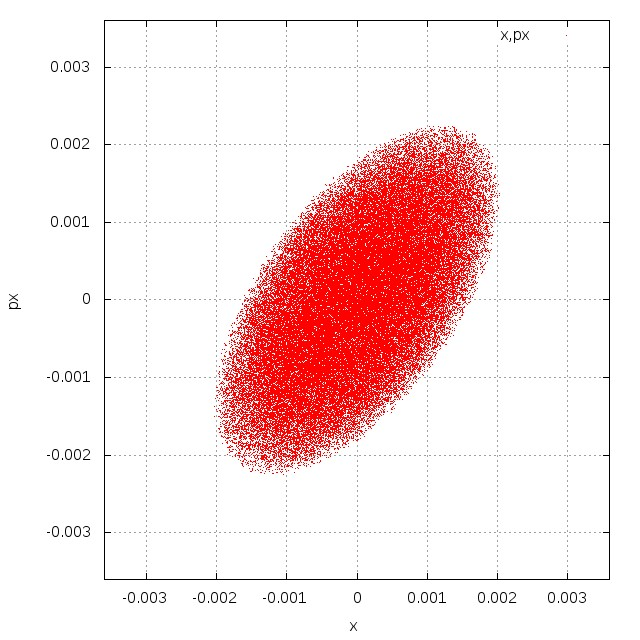
\includegraphics[width=\textwidth]{Img/WB_x_dx.jpg}
        \caption{Waterbag}
    \end{subfigure}
    \begin{subfigure}[b]{0.48\textwidth}
        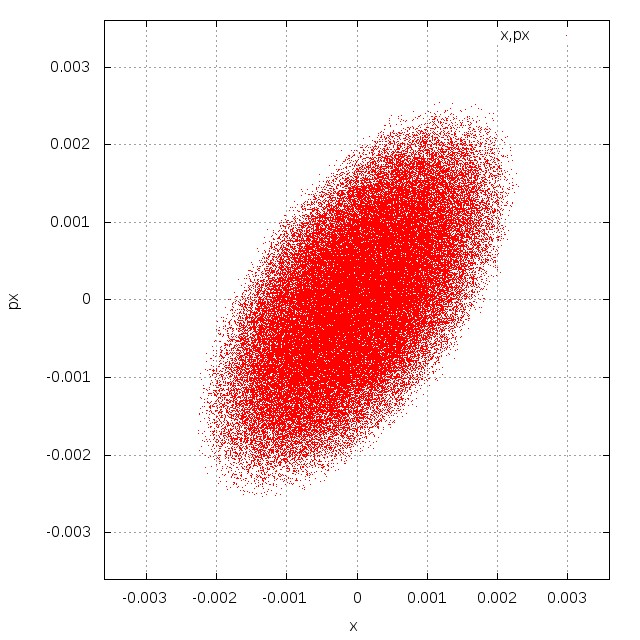
\includegraphics[width=\textwidth]{Img/PB_x_dx.jpg}
        \caption{Parabolic}
    \end{subfigure}
    \begin{subfigure}[b]{0.48\textwidth}
        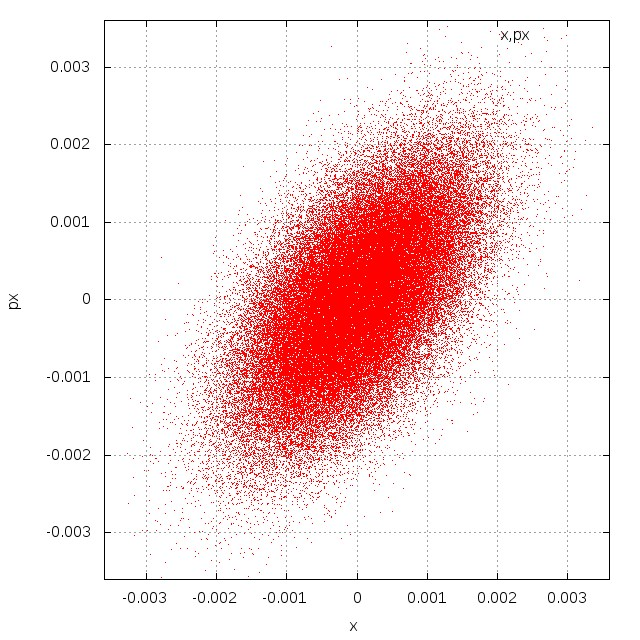
\includegraphics[width=\textwidth]{Img/GS_x_dx.jpg}
        \caption{Gaussian}
    \end{subfigure}
    \caption{同一均方根尺寸下的不同种类束团分布}\label{fig:distribution}
\end{figure}

程序主循环中的大部分都是并行化的,例如求解内场,推动粒子等。
最基本的,程序采用粒子并行策略,即每个线程处理不同的粒子。以粒子推动部分为例,如果粒子总数为160000,线程数为8,那么每个线程推动20000个粒子。
程序对可能发生线程冲突的部分,例如权重粒子,采用了其他的并行策略。除此之外,程序也使用了FFTW库的内部并行方法。


%程序也采用了一些其他的并行策略,以PIC求解Poisson方程为例,这部分需要4个独立的步骤来得到内部空间电荷场:
%\begin{enumerate}
%  \item 将粒子权重到网格,获得网格上的电荷密度;
%  \item 通过FFT求解网格上的Poisson方程,获得网格上的电势;
%  \item 对电势进行差分,获得网格上的电场;
%  \item 通过逆权重,得到粒子所在位置的电场。
%\end{enumerate}
%在第一步和第四步中,我们使用网格并行,即不同的线程处理不同的网格,这需要我们对粒子进行排序,以避免潜在的线程冲突。而在第二步和第三部中,主要的计算为傅里叶变换,程序使用了FFTW库的内部并行方法。

我们使用了一个4核的普通PC机进行性能测试,4线程运行的程序的速度是串行运行程序的3.6倍。关于程序的更大规模的并行问题,我们会在后文做进一步讨论。

\section{P-TOPO正确性校验}
\subsection{内场计算}
我们使用一个点电荷来测试PIC部分的正确性。使用的格点数目为 $128\times128\times64$。 横向边界为狄利克雷边界条件(第一类边界条件),纵向为周期性边界条件。 图\ref{fig:P_TOPO_verification1} 是P-TOPO 的结果与理论值的对比,其中左图为横向电势(X方向),右图为纵向电势(Z方向)。图中红色实线为程序通过PIC方法计算得到的电势场的大小,绿色虚线为理论值,可以看出,程序的结果与理论值非常吻合。

\begin{figure}[!htb]
    \centering
    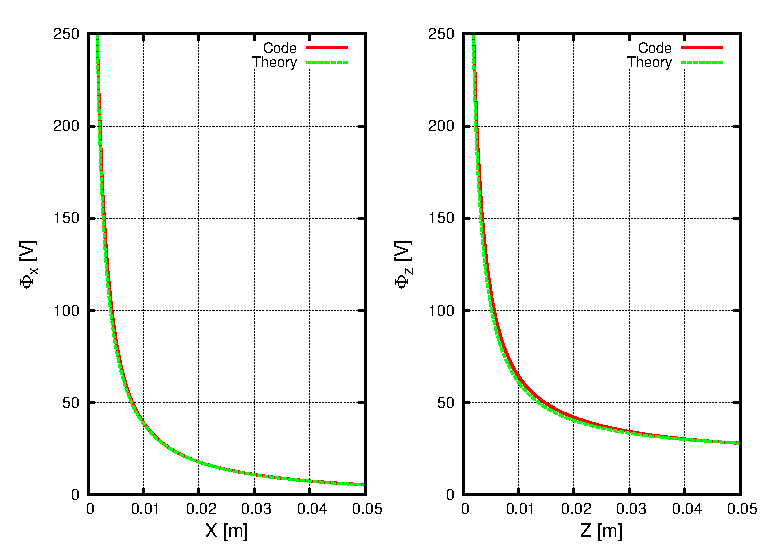
\includegraphics[width=0.8\textwidth]{Img/P_TOPO_verification1.eps}
    \caption{P-TOPO与理论值的点电荷电势对比}
    \label{fig:P_TOPO_verification1}
\end{figure}

\subsection{FD结构中与解析解的对比}
我们以束流在FD结构中束流的演化为例,来验证P-TOPO程序整体的正确性。连续束在周期聚焦结构中的束流包络方程可以表示为式\ref{eq:envelope}\cite{wangler1998particle,chen1994nonlinear}
\begin{equation}\label{eq:envelope}
  \frac{{{d}^{2}}R}{d{{z}^{2}}}+k_{0}^{2}R-\frac{{{\varepsilon }^{2}}}{{{R}^{3}}}-\frac{K}{R}=0
\end{equation}
其中$R$是束流横向均方根尺寸,$k_0$是聚焦强度,与外场力相关,$\varepsilon$为发射度,$K$是空间电荷力强度。束流的横向均方根尺寸与初始匹配和相移有关。
在这个验证中,计算空间电荷力的网格数目为64*64,我们使用10000个宏粒子在KV初始分布下,分别以0mA和15mA在周期性FD结构中前进,每个FD结构中推动400步。
图\ref{fig:P_TOPO_verification2}显示了由P-TOPO给出的束流均方根尺寸的演变和均方根包络方程的理论预期,其中图片下部浅蓝色线表示外部四级铁的聚焦强度,红色实线和绿色虚线分别为零流强下理论结果和P-TOPO程序计算结果,而蓝色实线和紫色虚线分别代表15mA流强下理论预期和P-TOPO计算结果。可以看出,无论是在零流强时还是15mA流强时,计算结果与理论值都保持高度一致,其中在15mA下束团演变的微小区别是因为包络方程计算中假定发射度为常数,而实际的PIC计算中发射度会发生变化。

\begin{figure}[!htb]
    \centering
    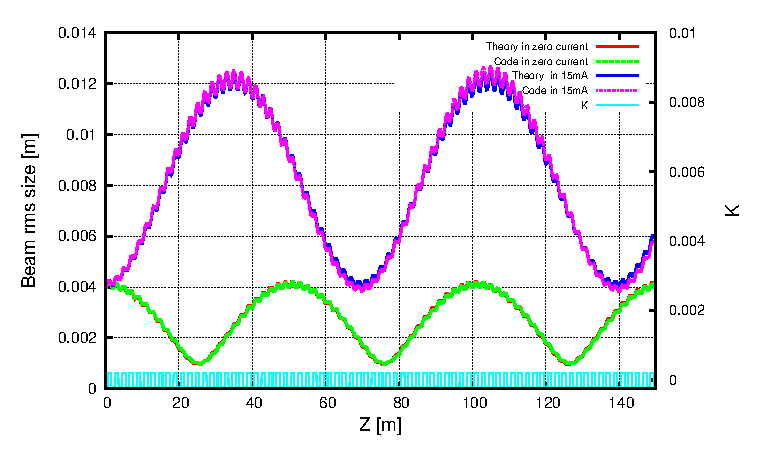
\includegraphics[width=0.8\textwidth]{Img/P_TOPO_verification2.eps}
    \caption{零流强和15mA时,P-TOPO结果与包络方程的对比}
    \label{fig:P_TOPO_verification2}
\end{figure}


%在本章中,首先,我们会介绍GPU程序的基本结构和并行策略。之后,我们做了一个GPU程序和CPU程序结果的对比,以验证程序的正确性。
%再后,我们展示了GPU程序的效率和在不同规模的问题下的加速比。
%最后,我们也实现了此程序在新的CPU架构,Knight Landing,上的并行化运行,并与GPU的运行效率进行了对比。

\section{PIC算法在GPU上的实现}
在\ref{section:PIC_algorithm}中我们介绍了基本的PIC算法。
PIC算法主要包括四部分:权重差值,解泊松方程,将场反权重到粒子,推动粒子。
在本章中,我们致力于在GPU上实现基于PIC算法的多粒子跟踪程序的并行化,提高程序的运行效率。
在GPU上实现PIC算法,主要难点在第一步权重差值上。第一步权重插值是将粒子逐个权重到网格上的过程,此步骤多线程并行运行时,会遇到不同线程相互竞争的问题(race condition),从而导致错误的结果。

线程竞争是指在程序中,协作的线程可能共享一些彼此都能读写的公用存储区,而竞争出现在当两个或多个线程同时访问同一内存地址,并且尝试写入数据的时候。由于线程调度器会以任意顺序运行多个线程,而我们无法得知线程尝试访问共享内存的顺序。因此,数据的最红结果会取决于线程调度器的算法,即多个线程“竞争”访问和改变数据。

图\ref{fig:PIC_weighting_threading}显示了PIC算法中权重差值部分的运算流程和多线程下可能会出现的竞争和冲突结果,其中蓝色点代表粒子,而绿色星状点代表与粒子相近的网格。使用多个线程运行权重插值时,通常使不同的线程处理不同的粒子。假设我们使用五个时钟锁步线程,如图\ref{fig:PIC_weighting_threading}中所示,线程A-E分别处理五个粒子。A,B,C三个线程并没有发生冲突,但是D线程和E线程会产生竞争,造成错误的运算结果。在第一个时钟周期内,线程D和E分别从同一内存地址M,读取格点原本的电荷量V;在第二个时钟周期,线程D读取粒子D的电荷并计算相应应该加到格点的电荷V+D,而线程E读取粒子E并计算得到V+E;在第三个时钟周期,线程D将V+D写入内存地址M,同时线程E将V+E写入同一内存地址M。但是两个写入都是错误,正确的结果应该是V+D+E。

\begin{figure}[!htb]
  \centering
  \begin{tabular}{|l|l|}
    \multicolumn{2}{c}{
    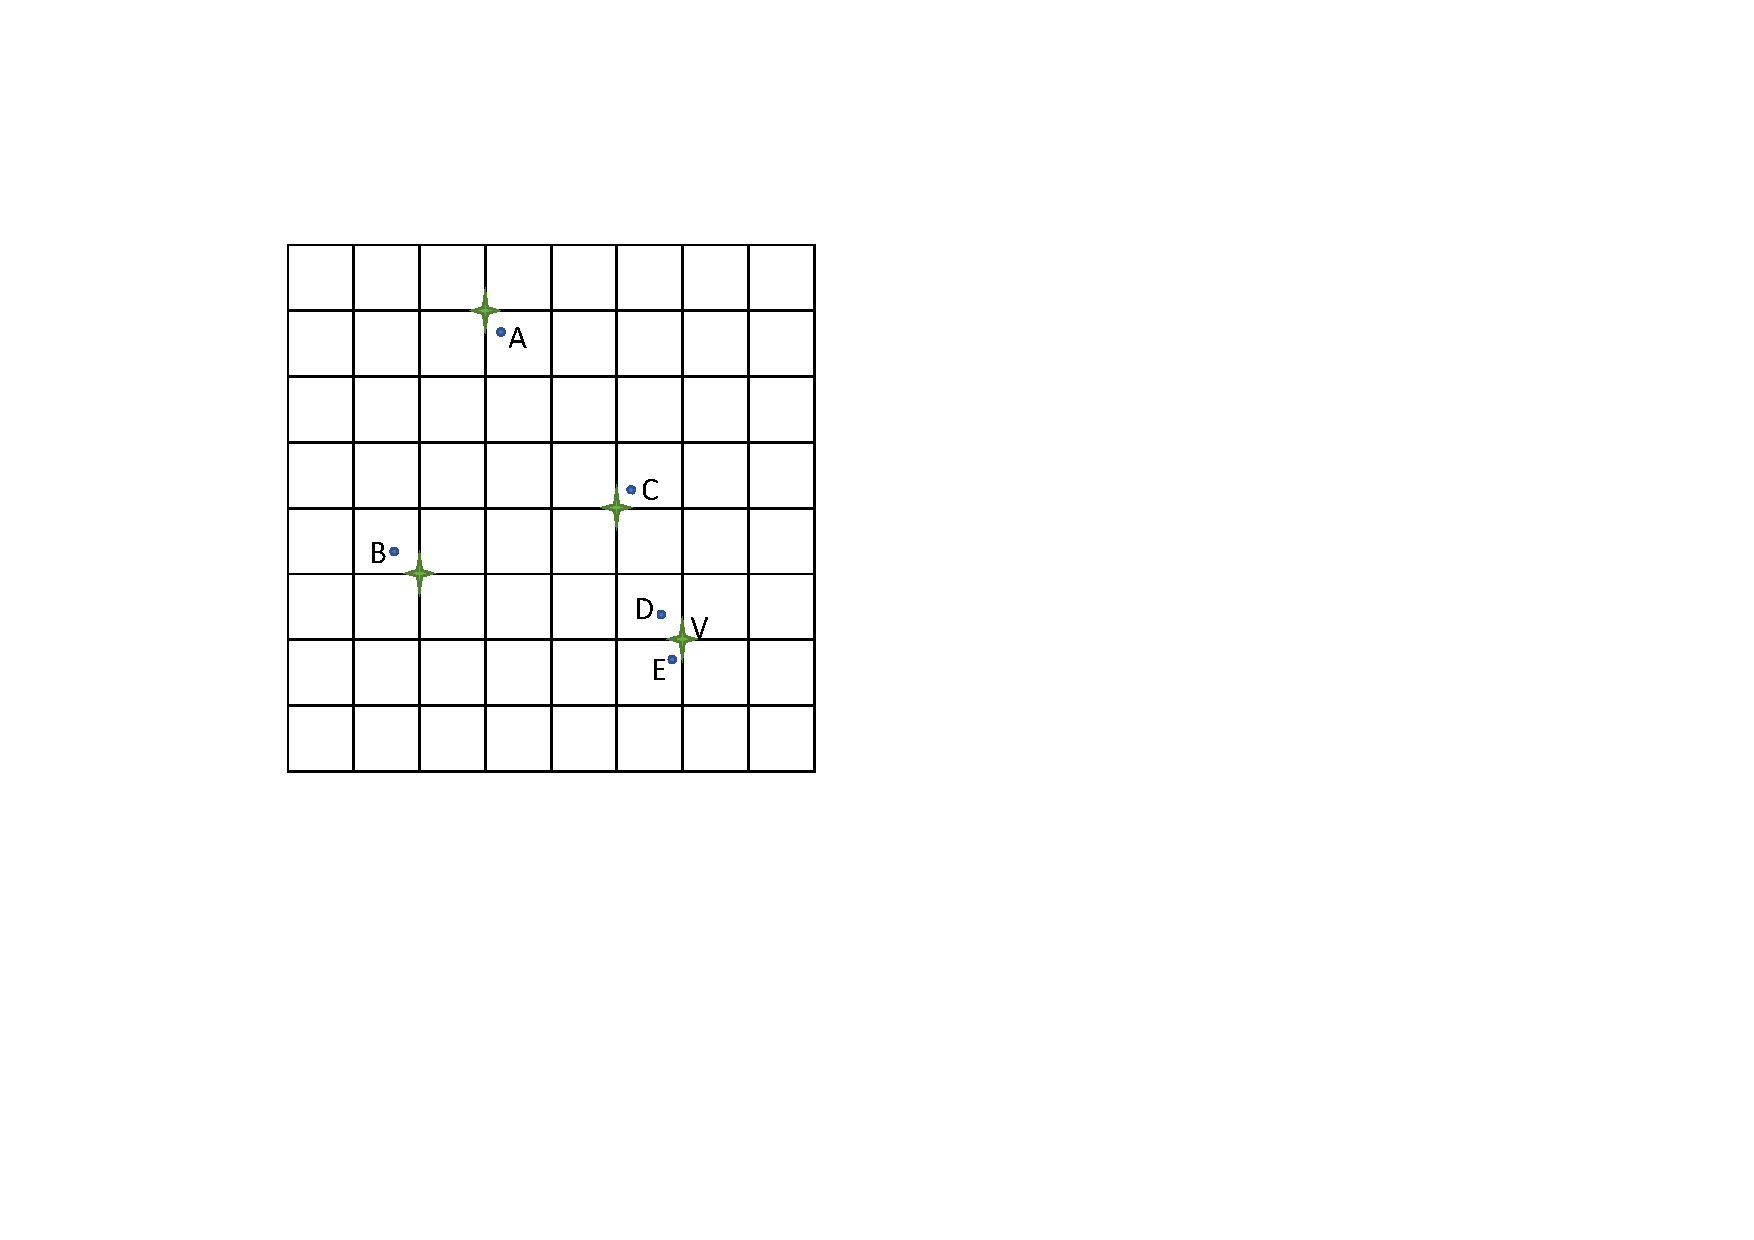
\includegraphics[width=0.65\textwidth]{Img/3PIC_weighting.pdf}} \\
  \end{tabular}
  \begin{tabular}{|l|l|}
    \hline
    Thread D & Thread E  \\
    \hline
    1D: Read variable V     & 1E: Read variable V     \\
    2D: Add D to variable V & 2E: Add E to variable V \\
    3D: Write back (V+D)    & 3E: Write back (V+E)    \\
    \hline
    \multicolumn{2}{c}{But it should be V + D + E!}
  \end{tabular}
  \caption{权重差值中的线程冲突}
  \label{fig:PIC_weighting_threading}
\end{figure}

为了避免线程之间的竞争和冲突,我们采取先将网格分块,再随后将网格上的电荷合并的做法。如图\ref{fig:PIC_tile}所示,绿色部分为一个区块,而一个线程单独处理一个区块。想要分块处理,粒子必须是有序的,这样才能使相应的线程找到所对应区域的粒子。所以在插值权重之前,我们需要对粒子进行排序(reorder)。假设区块数目为N,我们需要声明N个数组,以分别对应N个区块中的粒子。在程序初始阶段,我们将粒子数据拷贝到不同的区块数组中,并且在随后的每一步中,粒子可能改变位置,所以我们要对粒子重新排序,以确保粒子处于所对应的区块数组。用这种方法,每一个线程能够单独处理自己所分配的区块,从而避免了线程之间的竞争和冲突。加入了排序之后的PIC算法流程如图\ref{fig:PIC_flow_reorder}所示,其中,标识为红色部分为粒子排序,是PIC算法在GPU上并行运行所必须的前置步骤;而黄色部分的GPU算法和普通CPU算法有较大区别,我们在下面,对流程图种的黄色部分,即GPU上的PIC算法中的粒子排序,权重插值,解泊松方程,以及粒子推动做进一步讨论。

\begin{figure}[!htb]
    \centering
    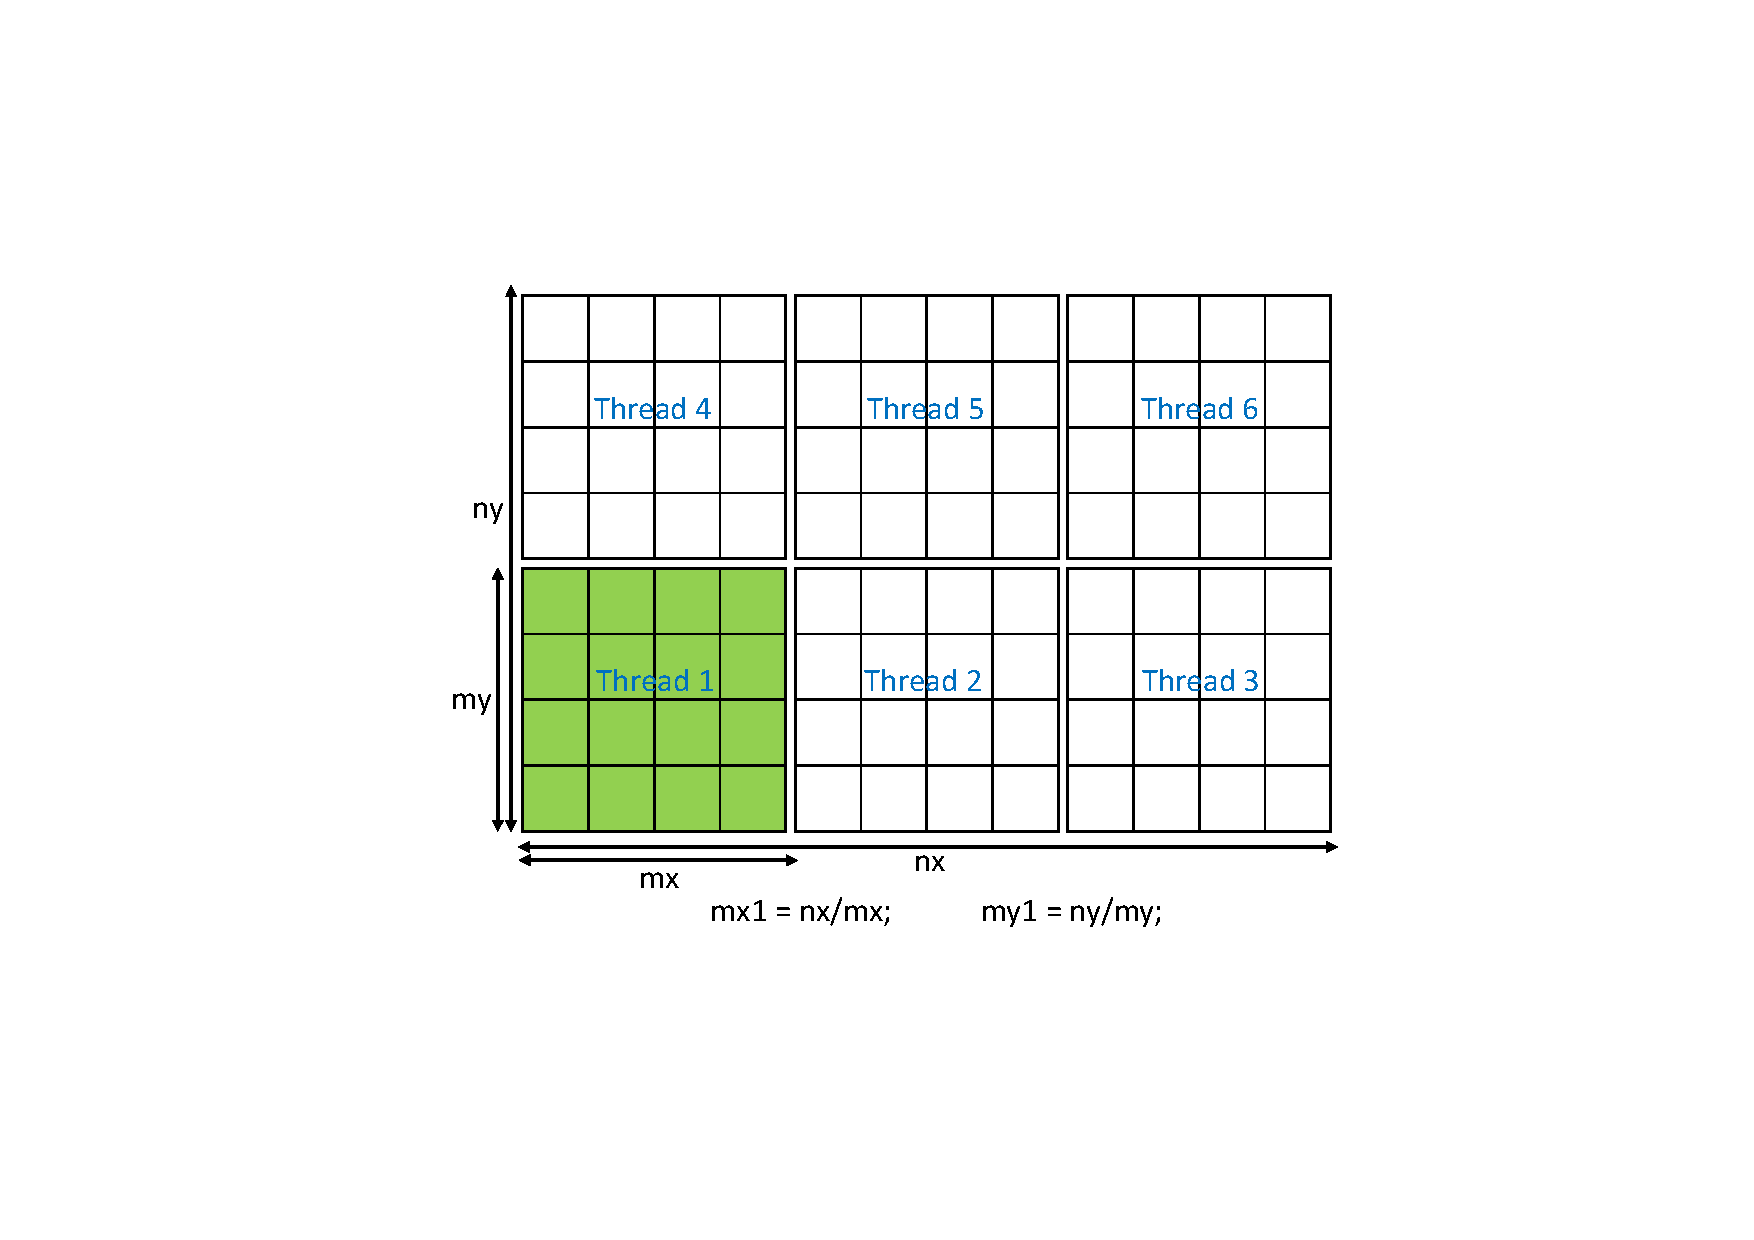
\includegraphics[width=0.85\textwidth]{Img/3PIC_tile.pdf}
    \caption{网格分块示意图}
    \label{fig:PIC_tile}
\end{figure}

\begin{figure}[!htb]
    \centering
    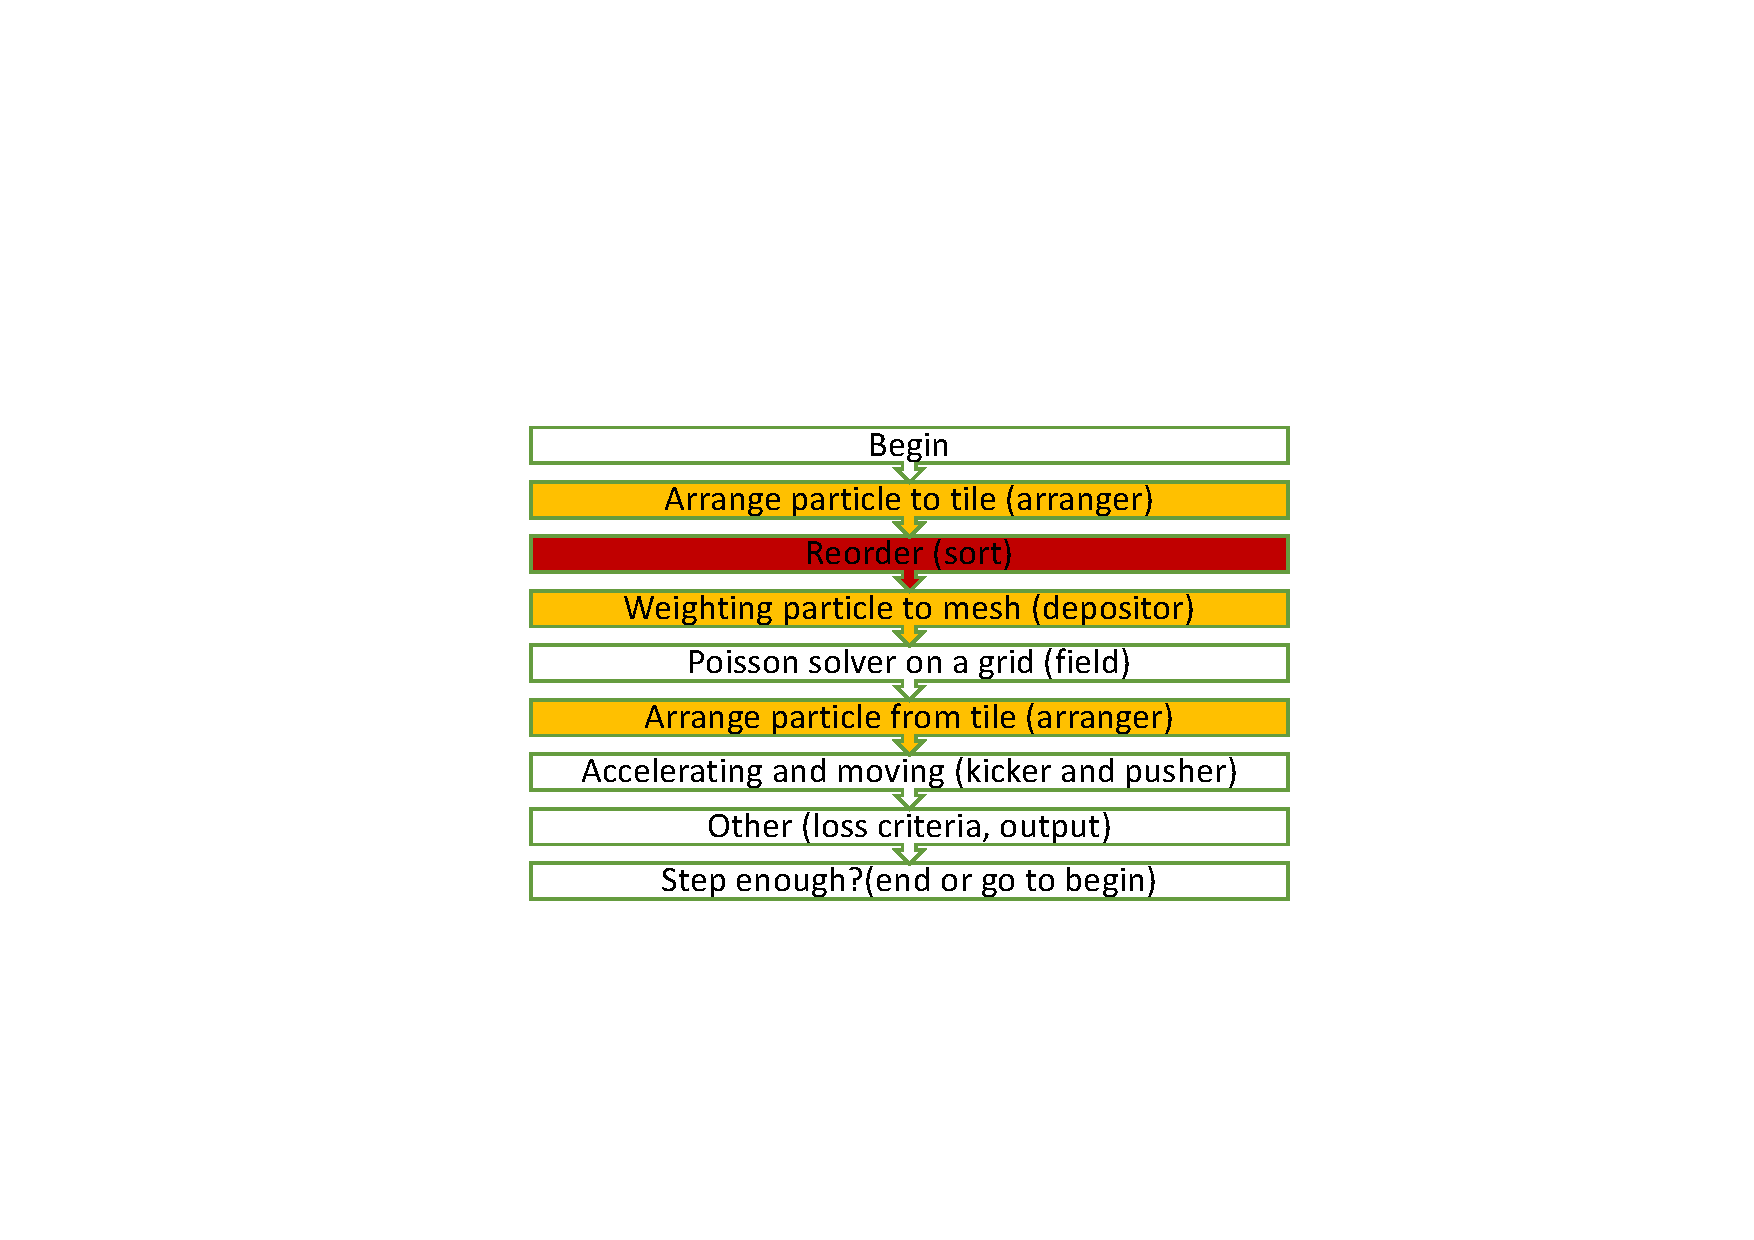
\includegraphics[width=0.75\textwidth]{Img/3PIC_flow_reorder.pdf}
    \caption{GPU上的PIC算法分段流程}
    \label{fig:PIC_flow_reorder}
\end{figure}



\subsection{粒子排序}
\label{section:PIC_GPU_reorder}
如上所述,GPU上PIC算法中,我们必须要将粒子在每一步进行重新排序,以避免线程竞争。排序在GPU中的实现并不直接,因为其高度不规则的并且难以并行执行。在这里,我们使用临时缓冲区作为中继,以实现粒子排序算法在GPU上的并行运行。
我们将整个网格划分为不同的区块,使每个线程只需处理对应的区块即可。例如,在一个网格数为$64 \times 64 \times 64$的模拟中,我们将其分割成大小为4*4*4的区块,总共$16 \times 16 \times 16$=4096个区块,这样我们可以避免线程的竞争。

在程序初始化的时候,我们首先需要为每一个区块声明数组并为其分配内存空间,如以下代码所示。
其中,我们根据实际使用的GPU的可用内存大小来确定每个区块的最大粒子数目。如果某一区块的粒子数目超过了最大粒子数,程序会报错并停止。在这种情况下,使用更少的粒子数目或者使用内存更大的显卡可以解决问题。
因为在实际模拟中,每个区块的粒子数一般并不相同,使用内存预分配会导致浪费很多内存空间。但是不同于CPU内存,在GPU上分配内存耗时很长,所以无法在每一步计算中根据实际情况来进行内存的分配,只能采用预分配的方法,以提高程序运行效率。
\begin{lstlisting}
  const int lth =BLOCKSIZE;
  const int dim =_dimension;
  int mth       = (mx1*my1*mz1-1)/lth+1;    //number of tiles

  double *ptc;       //tiled particle
  int    *kpic;      //number of particles in each tile
  int    *nhole;     //number of hole left
  int    *ncl;       //ndirec[k*26 + i]: number of particle going
                     //to destination i[0-26) from tile k
  double *pbuff;     //buffer for transfer particles

  //get the maximum number of particle according to the GPU memory size
  size_t freeMem,totalMem;
  cuda_SafeCall(cudaMemGetInfo(&freeMem,&totalMem));
  int npm = freeMem / 2 / sizeof(double) / dim / (mx1*my1*mz1);
  if(npm>numberOfParticle) npm = numberOfParticle;
  int MaxPtcTransf = npm / 2;


  //allocate memory for particle array
  size_t ptc_mem_size = sizeof(double)*lth*dim*npm*mth;
  cuda_SafeCall(cudaMalloc((void**) &ptc,     ptc_mem_size));

  //allocate memory for particle counting array
  size_t kpic_mem_size=sizeof(int)*mx1*my1*mz1;
  cuda_SafeCall(cudaMalloc((void**) &kpic,    kpic_mem_size));

  //allocate memory for holes at tiles array
  size_t nhole_mem_size = sizeof(double)*lth*2*(MaxPtcTransf+1)*mth;
  cuda_SafeCall((cudaMalloc((void**) &nhole,  nhole_mem_size));

  //allocate memory for particle buffer array
  size_t pbuff_mem_size = sizeof(double)*lth*dim*MaxPtcTransf*mth;
  cuda_SafeCall((cudaMalloc((void**) &pbuff,  pbuff_mem_size));

  //allocate memory for transferred particle counting array
  size_t ndirec_mem_size = sizeof(int)*mx1*my1*mz1*(3*3*3-1);
  cuda_SafeCall((cudaMalloc((void**) &ndirec, ndirec_mem_size));
\end{lstlisting}

在之后的每一步计算中,在空间电荷效应之前,我们都需要根据粒子空间位置对粒子进行排序,排序流程如图\ref{fig:PIC_reorder}所示:
\begin{figure}[!htb]
    \centering
    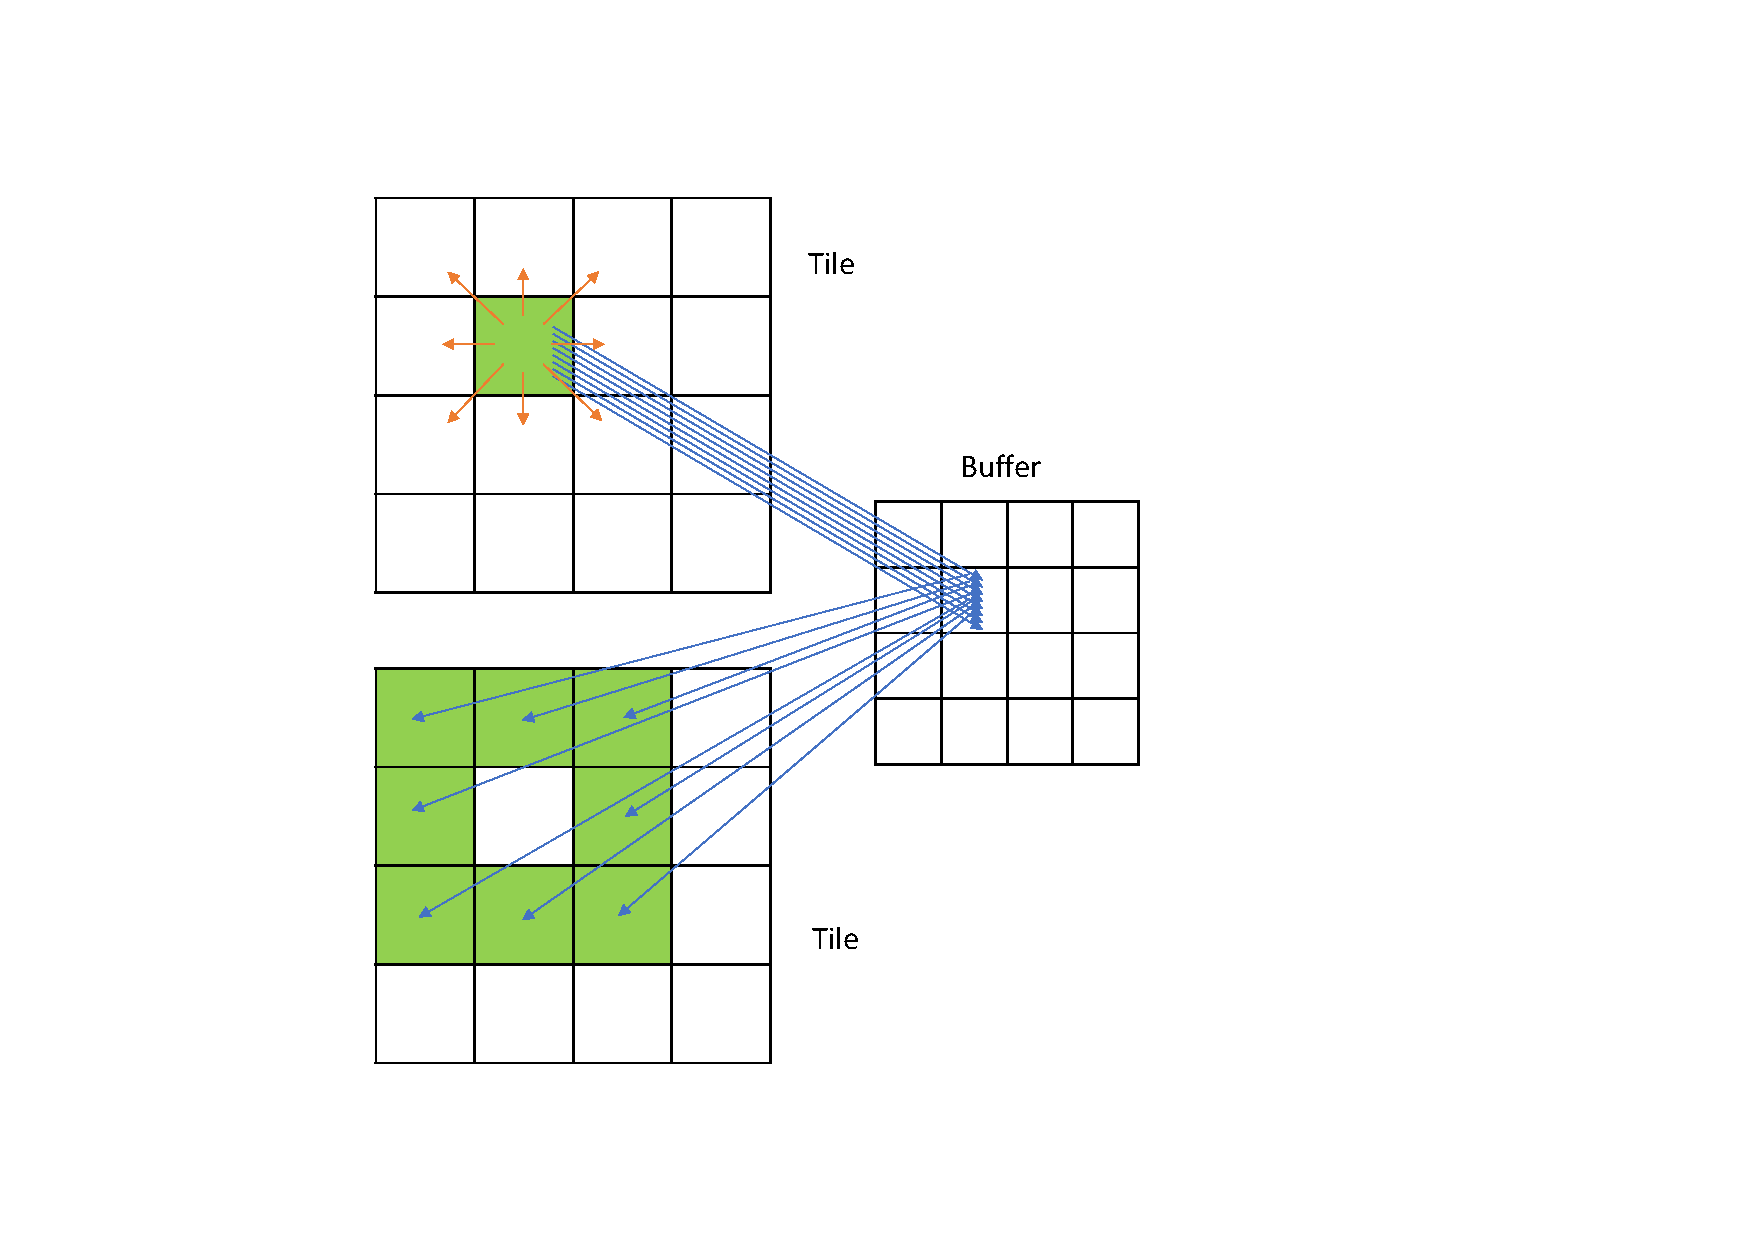
\includegraphics[width=0.75\textwidth]{Img/3PIC_reorder.pdf}
    \caption{粒子排序示意图}
    \label{fig:PIC_reorder}
\end{figure}

首先,每个线程统计对应区块中将要离开当前区块的粒子信息,并使用数组\verb"nhole"和\verb"ndirec"记录粒子的序号和每个方向的数目。如图\ref{fig:PIC_reorder}中黄色箭头所示。如上面代码所示,我们使用最大粒子数目的一半作为最大穿越数目,而\verb"nhole"已经根据最大穿越数目进行了内存预分配,同样的,如果离开当前区块的粒子数目超过了最大穿越数目,程序会报错停止,这时候需要使用更少的粒子数目或者更大的GPU内存。

之后,我们将离开当前区块的粒子信息拷贝到一个缓冲区\verb"pbuff"。作为全局内存,\verb"pbuff"同样根据最大穿越数目进行了内存预分配。\verb"ndirec"包括了每个方向上的粒子数目,对\verb"ndirec"进行迭代求和(running sum),我们可以得到每个方向上的内存初始位置,以便于将前往某个方向的粒子在\verb"pbuff"中连续排布。

最后,对于每个区块,经过第一步的统计,我们可以知道会有多少粒子进入,以及它们在\verb"pbuff"中的位置。在将粒子信息从\verb"pbuff"拷贝到当前区块\verb"ptc"的过程中,我们先填满因为粒子离开造成的空洞。如果如果进入的粒子数目大于空洞数目,即在所有空洞都被填满后,仍有粒子进入,我们将其写入在当前区块\verb"ptc"的最后;但如果进入的粒子数目小于空洞数目,即写入所有进入粒子后仍有空洞存在,则从本区块粒子数组\verb"ptc"尾部开始,依次移动粒子数据到空洞处。通过这种方式,粒子信息在内存中的连续性得到了保证。

我们对上述步骤做了一个简要总结,通过这些排序流程,使每个线程仅处理对应的区块,来确保不会出现线程竞争。

\begin{itemize}
  \item 首先,对本区块内的粒子进行遍历,将因为位置改变而不再属于本区块的粒子序号,以及其离开的方向记录下来,写入\verb"nhole" 和\verb"ndirec"。
  \item 其次,根据其序号和方向,将离开的粒子拷贝进入全局缓存区\verb"pbuff"。
  \item 最后,再根据相邻区块离开粒子的序号和方向,确定将要进入本区块的粒子,将缓存区内的数据拷贝到本区块。
\end{itemize}


\subsection{权重插值}
\label{section:PIC_GPU_depositor}
通过以上粒子重排,我们使得每一个区块的粒子相对独立,这样,我们可以使每个线程处理一个区块,从而避免了线程冲突的情况。
一个直接的权重插值流程如图所示\ref{fig:PIC_combine}:
\begin{itemize}
  \item 首先,每个线程将自己所处理的粒子权重到一个小网格上,得到本地的网格密度分布。
  \item 然后,我们将所有本地的密度分布结合到一起,得到全局密度分布。
\end{itemize}
\begin{figure}[!htb]
    \centering
    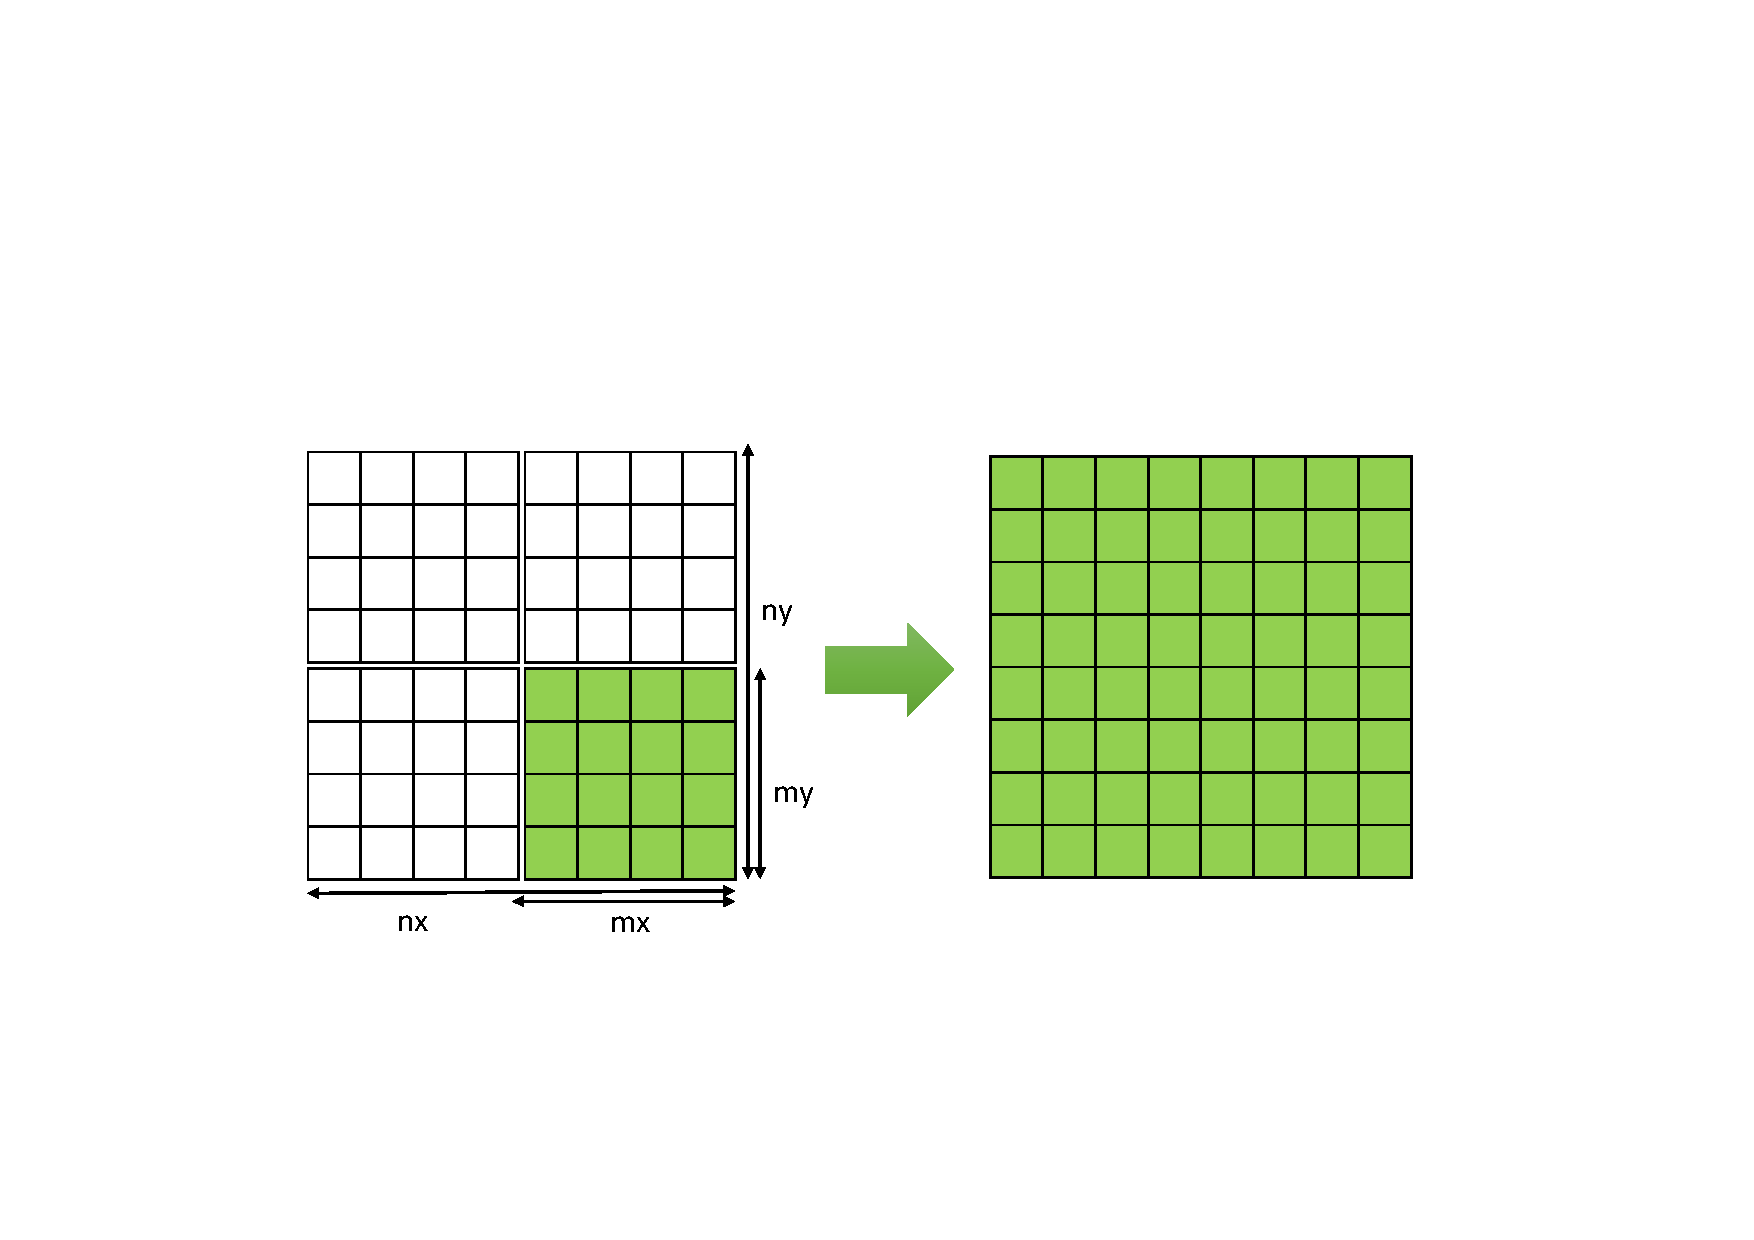
\includegraphics[width=0.9\textwidth]{Img/3PIC_combine.pdf}
    \caption{权重插值示意图}
    \label{fig:PIC_combine}
\end{figure}

上述为单GPU的权重差值方法,在使用多个GPU的时候,我们有两种方法:一种是使不同的GPU处理不同的空间域,在最后进行通讯,这种方法在CPU上的PIC程序中很常用,被称为“域分解”;另外一种是简单直接的使所有GPU做同样的工作,我们称这种模式为“复制模式”。
下面,我们使用一个例子对这两种方法进行比较,假设使用$64 \times 64 \times 64$个格点,区块大小为4*4*4,区块的数目为$16 \times 16 \times 16$,在TITAN上使用4个GPU运行。

\subsubsection{域分解模式}
在域分解模式中,每个GPU只需要处理相对应的域。假如区块数目为 $16 \times 16 \times 16$, 在4个GPU上运行的话,每个GPU需要处理的域的大小为$4 \times 16 \times 16$。但是,这种模式需要预先将粒子排序,使每个GPU只处理对应空间域内的粒子,因此需要额外的通讯和计算,具体步骤如下:
\begin{enumerate}
  \item GPU之间的粒子排序
  \begin{enumerate}
    \item 挑选粒子,每个线程处理一个区块,因此我们共有$4 \times 16 \times 16$=1024个线程。然而,在TITAN上每个GPU有2688个核,线程数小于核数,我们无法充分使用GPU。
    \item GPU之间信息交换
    \begin{enumerate}
      \item 从GPU内存拷贝到CPU内存,共需要拷贝$4 \times 16 \times 16$*(nGPU-1) * nPtcMax个粒子,其中nPtcMax个粒子为最大传输粒子数。
      \item CPU和CPU之间的信息交换,我们使用MPI\_send/receive,共需要交换$4 \times 16 \times 16$* (nGPU-1) *nPtcMax个粒子。
      \item 从CPU内存拷贝到GPU内存,共需要拷贝$4 \times 16 \times 16$*(nGPU-1) * nPtcMax个粒子。
    \end{enumerate}
  \end{enumerate}
  \item GPU内部的粒子排序,每个GPU的区块数目为$4 \times 16 \times 16$=1024,小于在每个 GPU 上的核数2688。
  \item GPU内部的权重差值,由于第一步进行了GPU之间的粒子排序,所以每个 GPU 上的粒子数目不同,格点数目为16*64*64。
  \item GPU之间的格点信息归约。
  \begin{enumerate}
    \item 从GPU内存拷贝到CPU内存,共需要拷贝16*64*64个格点。
    \item CPU和CPU之间的信息交换,我们使用MPI\_Allgether,共需要交换$64 \times 64 \times 64$个格点。
    \item 从CPU内存拷贝到GPU内存,共需要拷贝 $64 \times 64 \times 64$个格点。
  \end{enumerate}
\end{enumerate}

\subsubsection{复制模式}
在复制模式中,每个GPU进行同样的工作,同域分解模式相比,复制模式无法使用多GPU来节省计算时间,但是也无需在GPU之间进行粒子信息的交换。其流程如下所示,其中每一项和上面域分解模式相对。

\begin{enumerate}
  \item 无需GPU之间排序
  \item GPU内部的粒子排序,每个GPU的区块数目为$16 \times 16 \times 16$=4096,大于在每个 GPU上的核数2688。
  \item GPU内部的权重差值,每个GPU上的粒子数目相同。
  \item GPU之间的格点信息归约。
  \begin{enumerate}
    \item 从GPU内存拷贝到CPU内存,共需要拷贝$64 \times 64 \times 64$个格点。
    \item CPU和CPU之间的信息交换,我们使用MPI\_Allreduce,共需要交换 $64 \times 64 \times 64$个格点。
    \item 从CPU内存拷贝到GPU内存,共需要拷贝$64 \times 64 \times 64$个格点。
  \end{enumerate}
\end{enumerate}

可以看出,两个模式相比较的话,域分解模式在第一步中有了很多额外的通讯,在第二步与第三步中能够使用更少的格点数。然后,使用通讯时间来换取更少的计算量并不能带来效率的提升,而且,在域分解模式下,我们并不能充分利用GPU。因此,在我们的代码中以及接下来的性能测试中,我们均采用“复制模式”。

\subsection{泊松方程}
\label{section:PIC_GPU_Poisson}
在将粒子权重到网格上之后,下一步即解网格上的泊松方程。在单GPU上运行的版本我们在此不再赘述,而在多GPU上的并行版本和权重差值相似,也存在两种方法:一种是参考经典的CPU上的PIC程序,使用不同的GPU处理不同的空间域,即“域分解模式”;另外一种是简单直接的使所有GPU做同样的工作,即“复制模式”。由于解泊松方程的运算量较大,是PIC方法中很重要的一步,我们对两种模式都进行了实现并进行了比较。

\subsubsection{域分解模式与复制模式}
域分解的优点在于,通过使用不同的GPU处理不同的空间域,每个GPU可以降低计算量,从而提高程序运行速度;缺点也很明显,域分解模式需要不同GPU之间的信息交换,而在目前GPU与GPU之间,特别是在不同节点之间,并不能直接进行信息交换,而是必须通过CPU来进行,即信息交换需要三步:
\begin{enumerate}
  \item 从GPU内存拷贝到CPU内存。
  \item CPU和CPU之间的通过MPI进行信息交换。
  \item 从CPU内存拷贝到GPU内存。
\end{enumerate}

如小节\ref{section:PIC_FFT}所示,求解泊松方程中最主要的部分是使用傅里叶变换(FFT)。在GPU代码中,我们使用NVIDIA公司的CUDA快速傅里叶变换库(cuFFT)\cite{nvidia2010cufft}在进行变换。在求解多GPU上的3维傅里叶变换时,最好是在三个方向分别做1维的傅里叶变换,并在每次变换之间对数据进行转置。

假设在X,Y,Z三个方向上的格点数分别为$N_x$,$N_y$,$N_z$,那么当执行X方向的傅里叶变换的时候,变换的数组长度即为$N_x$,变换的次数为$N_y \times N_z$。 以使用四个GPU为例,那么1号GPU需要处理的数据为\verb'rho'[$N_x$][$0 \rightarrow \frac{N_y}{4}$][$N_z$],2号GPU需要处理的数据为\verb'rho'[$N_x$][$\frac{N_y}{4} \rightarrow 2\frac{N_y}{4}$][$N_z$],3号GPU需要处理的数据为\verb'rho'[$N_x$][$2\frac{N_y}{4}\rightarrow 3\frac{N_y}{4}$][$N_z$],4号GPU需要处理的数据为\verb'rho'[$N_x$][$3\frac{N_y}{4}\rightarrow N_y$][$N_z$]。每个GPU只需要进行$\frac{N_y}{4} \times N_z$ 次变换即可。理想情况下,和单GPU运行相比,使用4个GPU运行只需要花费1/4的时间。

在X方向的傅里叶变换结束后,我们需要其他的数据来进行Y方向的运算,目前每个GPU上的数据为\verb'rho'[$N_x$][$(n-1)\frac{N_y}{4}\rightarrow (n)\frac{N_y}{4}$][$N_z$],而进行Y方向的傅里叶变换需要的数据为\verb'rho'[$(n-1)\frac{N_x}{4}\rightarrow (n)\frac{N_x}{4}$][$N_y$][$N_z$]。我们必须对数据求转置并在GPU之间进行数据交换。而由于目前GPU与GPU之间并不能直接进行数据交换,我们不需将GPU中的数据拷贝回CPU内存中,并在CPU端进行通讯,这将需要额外的时间。所以域分解模式相比复制模式的效率高低将取决于额外的通信时间与降低的运算时间的比较。

以$64 \times 64 \times 64$个格点数,使用4个GPU为例,域分解模式求解泊松方程的具体步骤可以表示如下:
\begin{enumerate}
  \item X方向的FFT
  \begin{enumerate}
    \item 拷贝到GPU(64*16*64)
    \item FFT(64*16*64)
    \item 拷贝到CPU(64*16*64)
  \end{enumerate}
  \item 转置及CPU与CPU之间的信息通讯
  \item Y方向的FFT
  \begin{enumerate}
    \item 拷贝到GPU(64*16*64)
    \item FFT(64*16*64)
    \item 拷贝到CPU(64*16*64)
  \end{enumerate}
  \item 转置及CPU与CPU之间的信息通讯
  \item Z方向的FFT
  \begin{enumerate}
    \item 拷贝到GPU(64*16*64)
    \item FFT(64*16*64)
    \item 拷贝到CPU(64*16*64)
  \end{enumerate}
\end{enumerate}

相比较而言,复制模式的步骤为:
\begin{enumerate}
  \item X方向的FFT($64 \times 64 \times 64$)
  \item Y方向的FFT($64 \times 64 \times 64$)
  \item Z方向的FFT($64 \times 64 \times 64$)
\end{enumerate}
\subsubsection{单GPU测试}
我们在单GPU上对域分解模式进行了测试,并统计了每一部分所花费的时间。测试的格点数为$64 \times 64 \times 64$,每部分所花费的时间如表\ref{tab:1GPU_Poisson},表中的单位为秒,每部分占比如图\ref{fig:1GPU_Poisson}。

\begin{table}[!htbp]
    \centering
    \footnotesize% fontsize
    \setlength{\tabcolsep}{4pt}% column separation
    \renewcommand{\arraystretch}{1.2}%row space
    \begin{tabular}{lc}
        \hline\hline
        从CPU拷贝到GPU    & 1.306     \\
        \hline
        从GPU拷贝到CPU    & 2.979     \\
        \hline
        FFT计算           & 0.487     \\
        \hline
        转置和通讯        & 3.772     \\
        \hline
        总计              & 8.544    \\
        \hline\hline
    \end{tabular}
    \caption{单GPU域分解模式解泊松方程}
    \label{tab:1GPU_Poisson}
\end{table}

\begin{figure}[!htb]
    \centering
    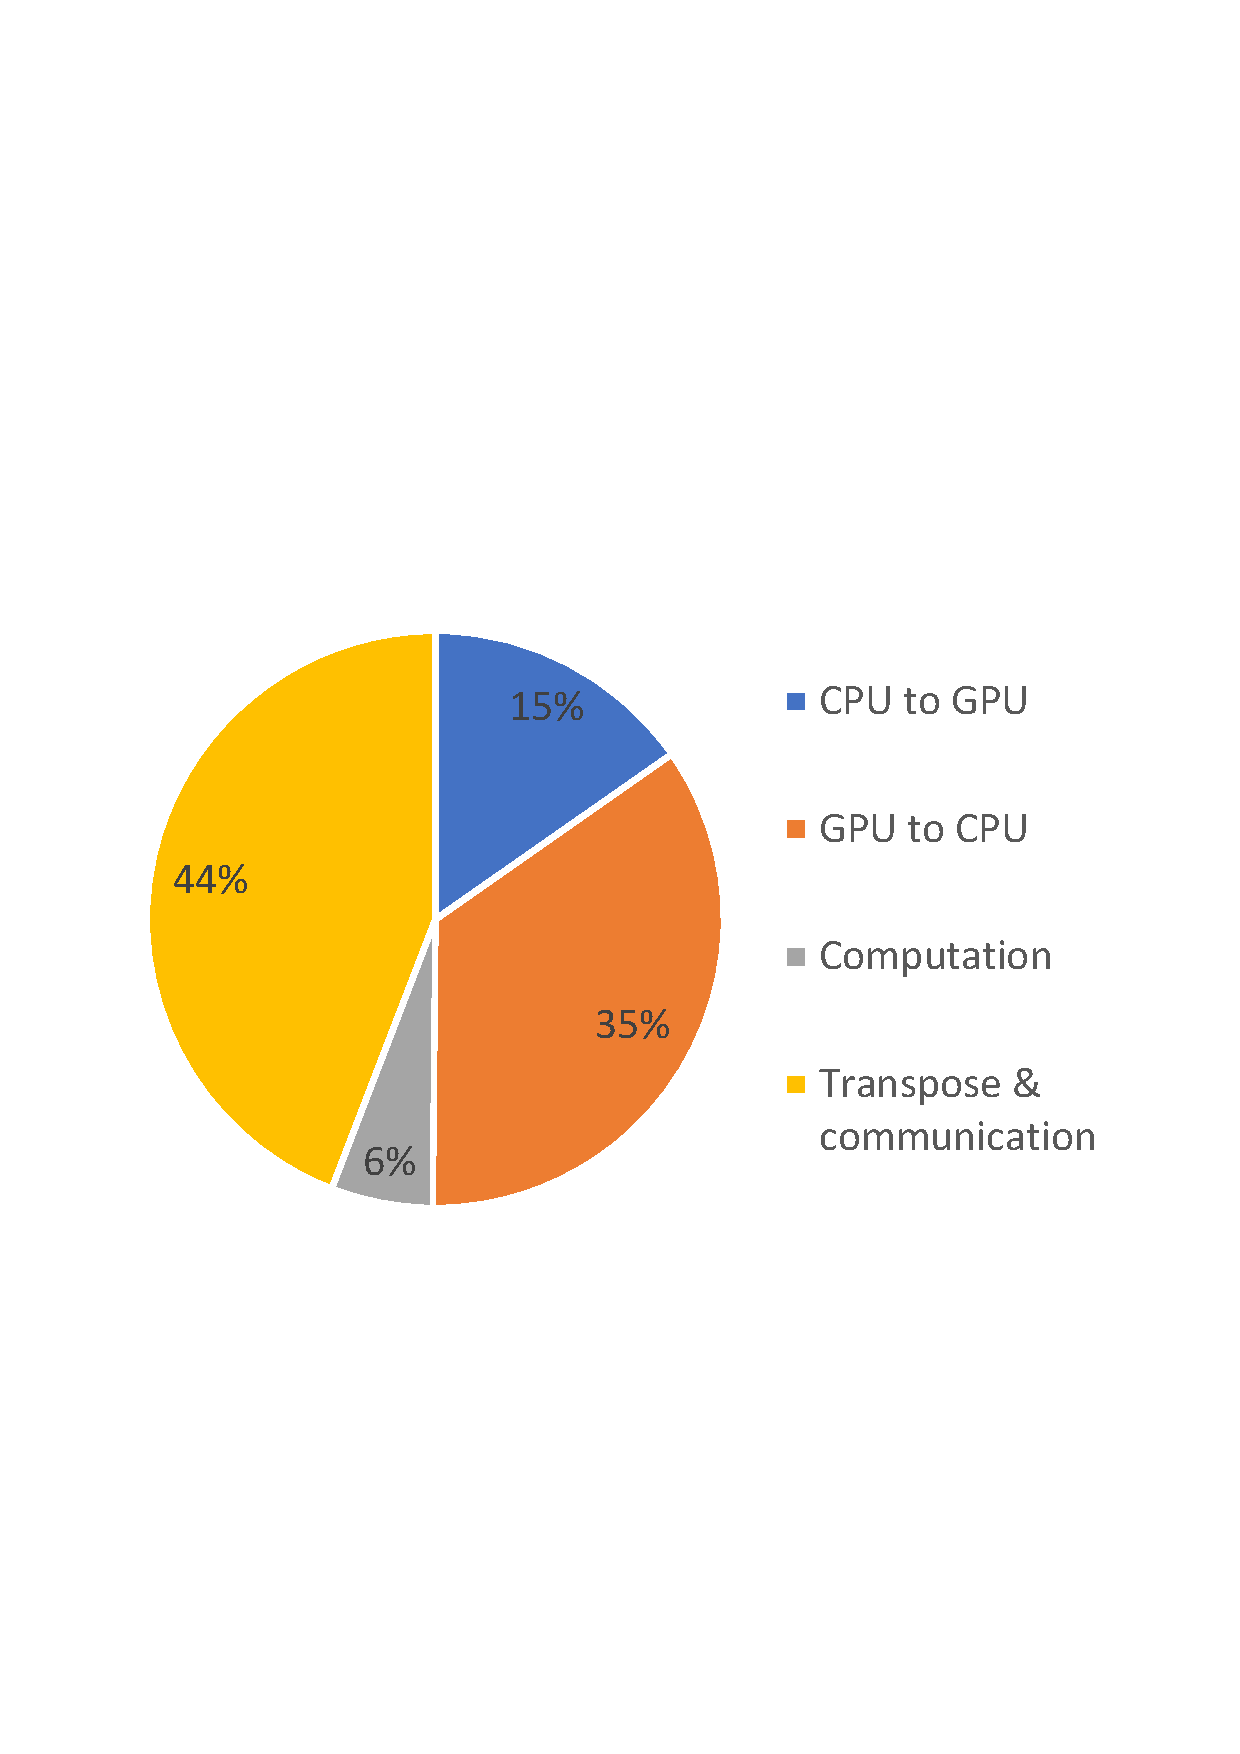
\includegraphics[width=0.7\textwidth]{Img/domain_decomposition_1GPU.pdf}
    \caption{单GPU域分解模式解泊松方程各部分时间占比}\label{fig:1GPU_Poisson}
\end{figure}

可以看出,FFT计算所花的时间为0.487秒,相比于额外增加的数据拷贝时间1.306 + 4.627 = 4.933秒,其占比非常小,仅仅占总时间的6\%。

多GPU的一种方式是使用同一节点内使用多个GPU,因为节点内的总线宽度限制,数据拷贝时间并不会随着使用GPU数目的增加而明显减少。而复制模式只需要花费FFT计算的时间,因为FFT计算花费的时间0.487秒远小于数据拷贝的时间4.933秒,所以即使在理想情况下使用N个GPU时FFT计算的时间减少到原来的1/N,域分解模式的总时间依然是比复制模式要大。

多GPU的另一种使用跨节点的多个GPU,即每个节点有1个GPU,通过使用多个节点来使用多个GPU,这也是目前超级计算机TITAN的运行模式。总线宽度会随着节点数增加而增加,所以数据拷贝时间会下降,假设其下降为现行的,即在N个节点上运行的话拷贝数据时间只有原来的1/N,则总时间将会是 $4.933/N+0.487/N$,如果我们想要取得优于复制模式的速度,即 $4.933/N+0.487/N<0.487$, GPU数目必须大于11。类似的,如果我们想要取得两倍的速度,GPU数目必须大于22。然而,这个计算忽略了CPU和CPU之间的通讯时间,一般来说,节点间的通讯时间随着节点数目增加而增加,因此我们很难取得理想情况的加速比。

下面,我们分别对节点内多GPU和跨节点GPU进行测试。

\subsubsection{单节点多GPU测试}
在同一节点中,我们进行了格点数为$64 \times 64 \times 64$的多GPU测试,表\ref{tab:2GPU_Poisson}是各个部分所花费的时间,以及和单GPU时的对比。可以看出,双GPU的总时间更大了,由8.544秒增加到了9.537秒。其中,FFT计算的时间有0.487秒减少到了0.249秒,几乎减少了一半,证明了多GPU对于减少纯FFT计算时间是确实有效的;对于数据拷贝时间,双GPU略有减少,大概减少了三分之一;总时间中增加的部分来源于转置和通讯的时间,几乎增加了一倍。
\begin{table}[!htbp]
    \centering
    \footnotesize% fontsize
    \setlength{\tabcolsep}{4pt}% column separation
    \renewcommand{\arraystretch}{1.2}%row space
    \begin{tabular}{lcc}
        \hline\hline
                          & 1GPU    & 2GPU   \\
        \hline\hline
        从CPU拷贝到GPU    & 1.306   & 0.817  \\
        \hline
        从GPU拷贝到CPU    & 2.979   & 1.991  \\
        \hline
        FFT计算           & 0.487   & 0.249  \\
        \hline
        转置和通讯        & 3.772   & 6.480  \\
        \hline
        总计              & 8.544   & 9.537  \\
        \hline\hline
    \end{tabular}
    \caption{单节点双GPU域分解模式解泊松方程}
    \label{tab:2GPU_Poisson}
\end{table}

\subsubsection{跨节点多GPU测试}
我们使用超级计算机泰坦(Titan)来进行域分解模式下的解泊松方程在跨节点多GPU上的效率。泰坦是一台由克雷公司承建的超级电脑,置放于美国能源部下属的橡树岭国家实验室中,使用由超微半导体提供的皓龙(Opteron)处理器链接英伟达提供的Tesla运算用GPU以进行协同运算。

首先,我们测试了常用的$64 \times 64 \times 64$个格点下,域分解模式下解泊松方程所花费的时间随GPU个数的变化,如图\ref{fig:TITAN_GPU_Poisson64}所示,图中蓝线为总时间,各个柱代表各个部分所花费的时间,在GPU数目很大时,图中不清楚部分可以参考表\ref{tab:TITAN_GPU_Poisson64}。

可以看出,花费的总时间随着GPU数目增加而逐渐减少,并在32个GPU的时候到达最小值,随后开始逐渐增加。其中,拷贝数据所花费的时间基本随着GPU的数目线性减少;而通讯所花费的时间先随着GPU数目增加而逐渐减少,到达极值后又开始逐渐增加,此时通讯时间占程序所花费的时间的绝大部分;FFT计算所花费的时间随着GPU数目的增加而逐渐减少,但是FFT计算占总时间的百分比很小。

\begin{figure}[!htb]
  \centering
  \begin{tabular}{|l|l|}
    \multicolumn{2}{c}{
    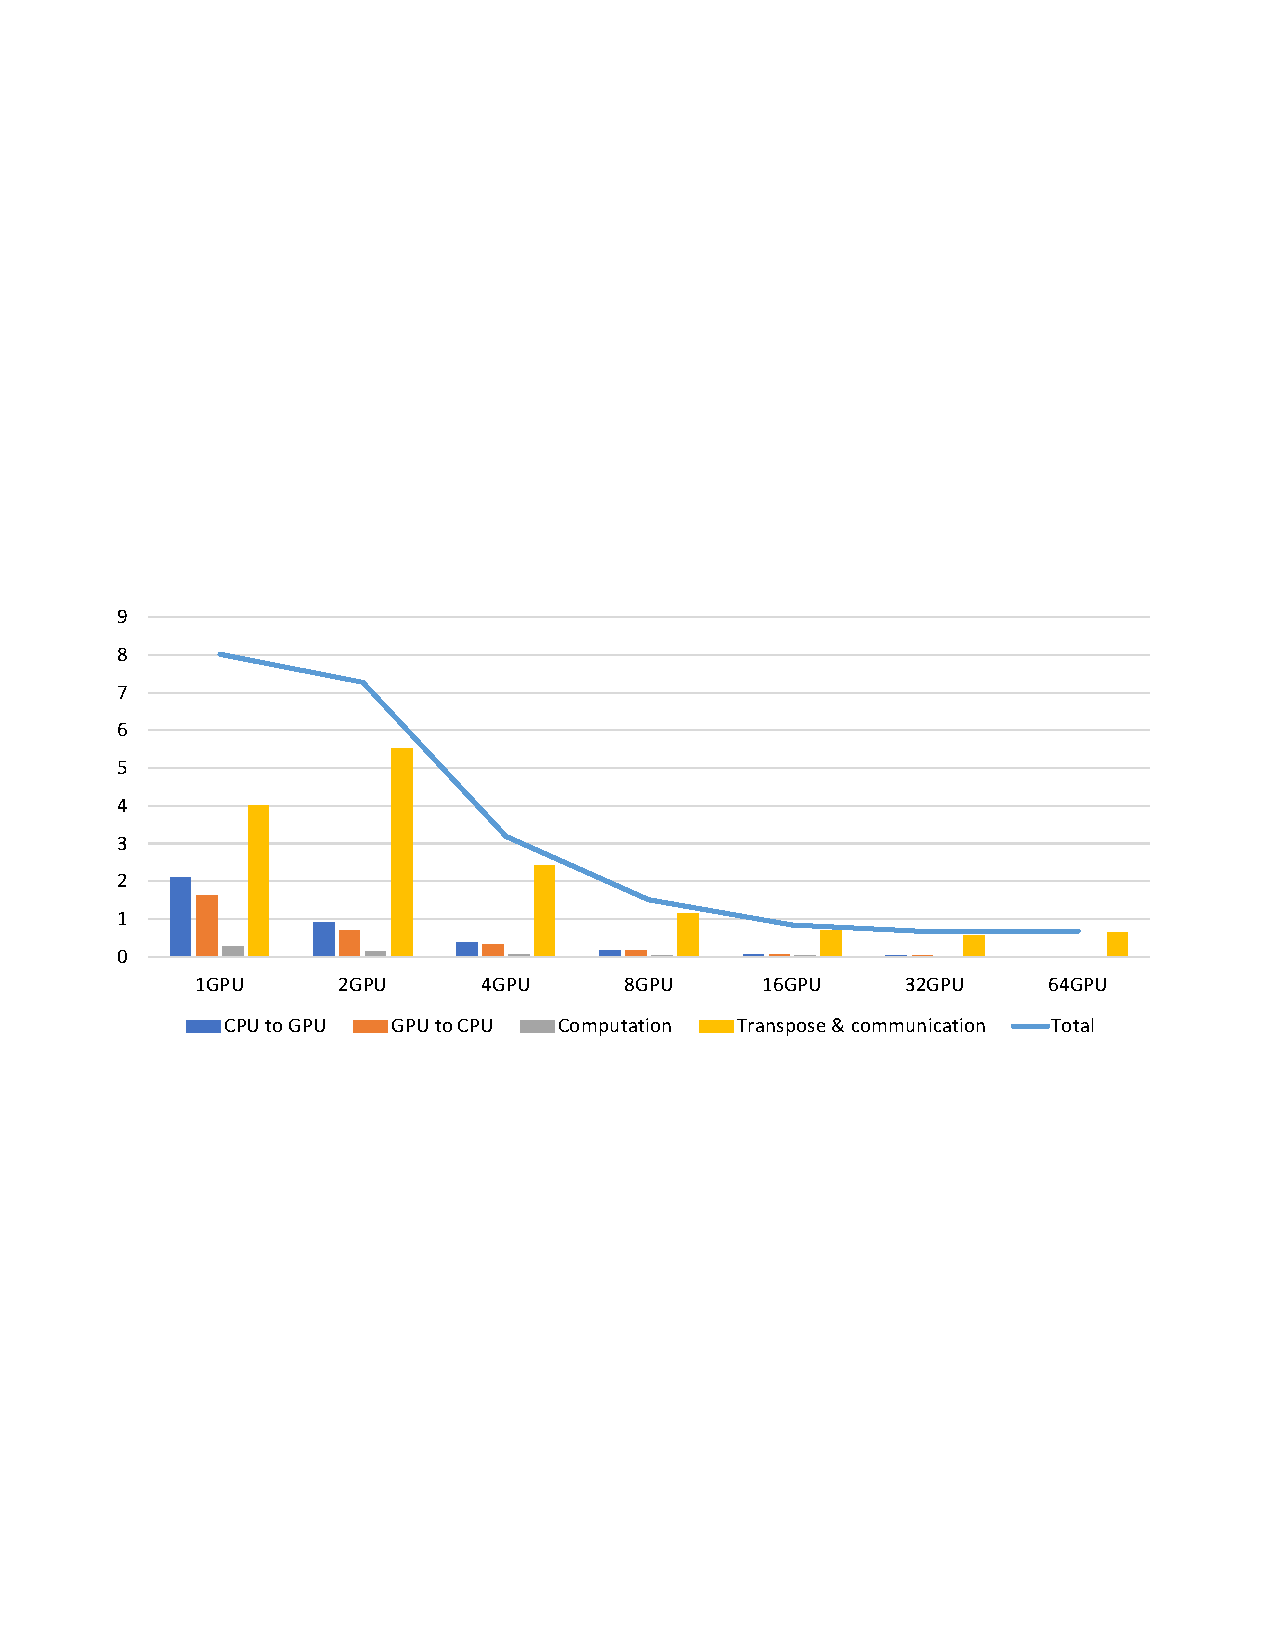
\includegraphics[width=0.9\textwidth]{Img/domain_decomposition_Titan64.pdf}} \\
  \end{tabular}
  \caption{$64 \times 64 \times 64$格点下,跨节点多~GPU~域分解模式解泊松方程时间随~GPU~个数的变化}
  \label{fig:TITAN_GPU_Poisson64}
\end{figure}

\begin{table}
  \centering
  \begin{tabular}{|l|c|c|c|c|c|c|c|}
    \hline
    GPU数目	    &1	    &2	    &4	    &8 	    &16	    &32  	&64   \\
    \hline
    CPU to GPU	&2.111	&0.922	&0.390	&0.158	&0.061	&0.031	&0.0155 \\
    GPU to CPU	&1.618	&0.694	&0.314	&0.167	&0.066	&0.033	&0.0158 \\
    FFT计算  	    &0.266	&0.136	&0.069	&0.039	&0.024	&0.017	&0.0150 \\
    转置和通讯	&4.02	&5.521	&2.415	&1.146	&0.691	&0.572	&0.6320 \\
    总计	        &8.015	&7.273	&3.188	&1.51	&0.842	&0.653	&0.6783 \\
    \hline
  \end{tabular}
  \caption{$64 \times 64 \times 64$格点下,跨节点多GPU 域分解模式解泊松方程各部分所用时间}
  \label{tab:TITAN_GPU_Poisson64}
\end{table}

我们也测试了更多格点数目时的情况,格点数目越多,所需要的计算量越大。当格点数为$128 \times 128 \times 128$时,程序在不同的GPU数目下消耗的时间如图\ref{fig:TITAN_GPU_Poisson128}和表\ref{tab:TITAN_GPU_Poisson128}所示,其整体的趋势和$64 \times 64 \times 64$时类似,因为更大的计算量,其总时间在使用128个GPU时到达最小值。

\begin{figure}[!htb]
  \centering
  \begin{tabular}{|l|l|}
    \multicolumn{2}{c}{
    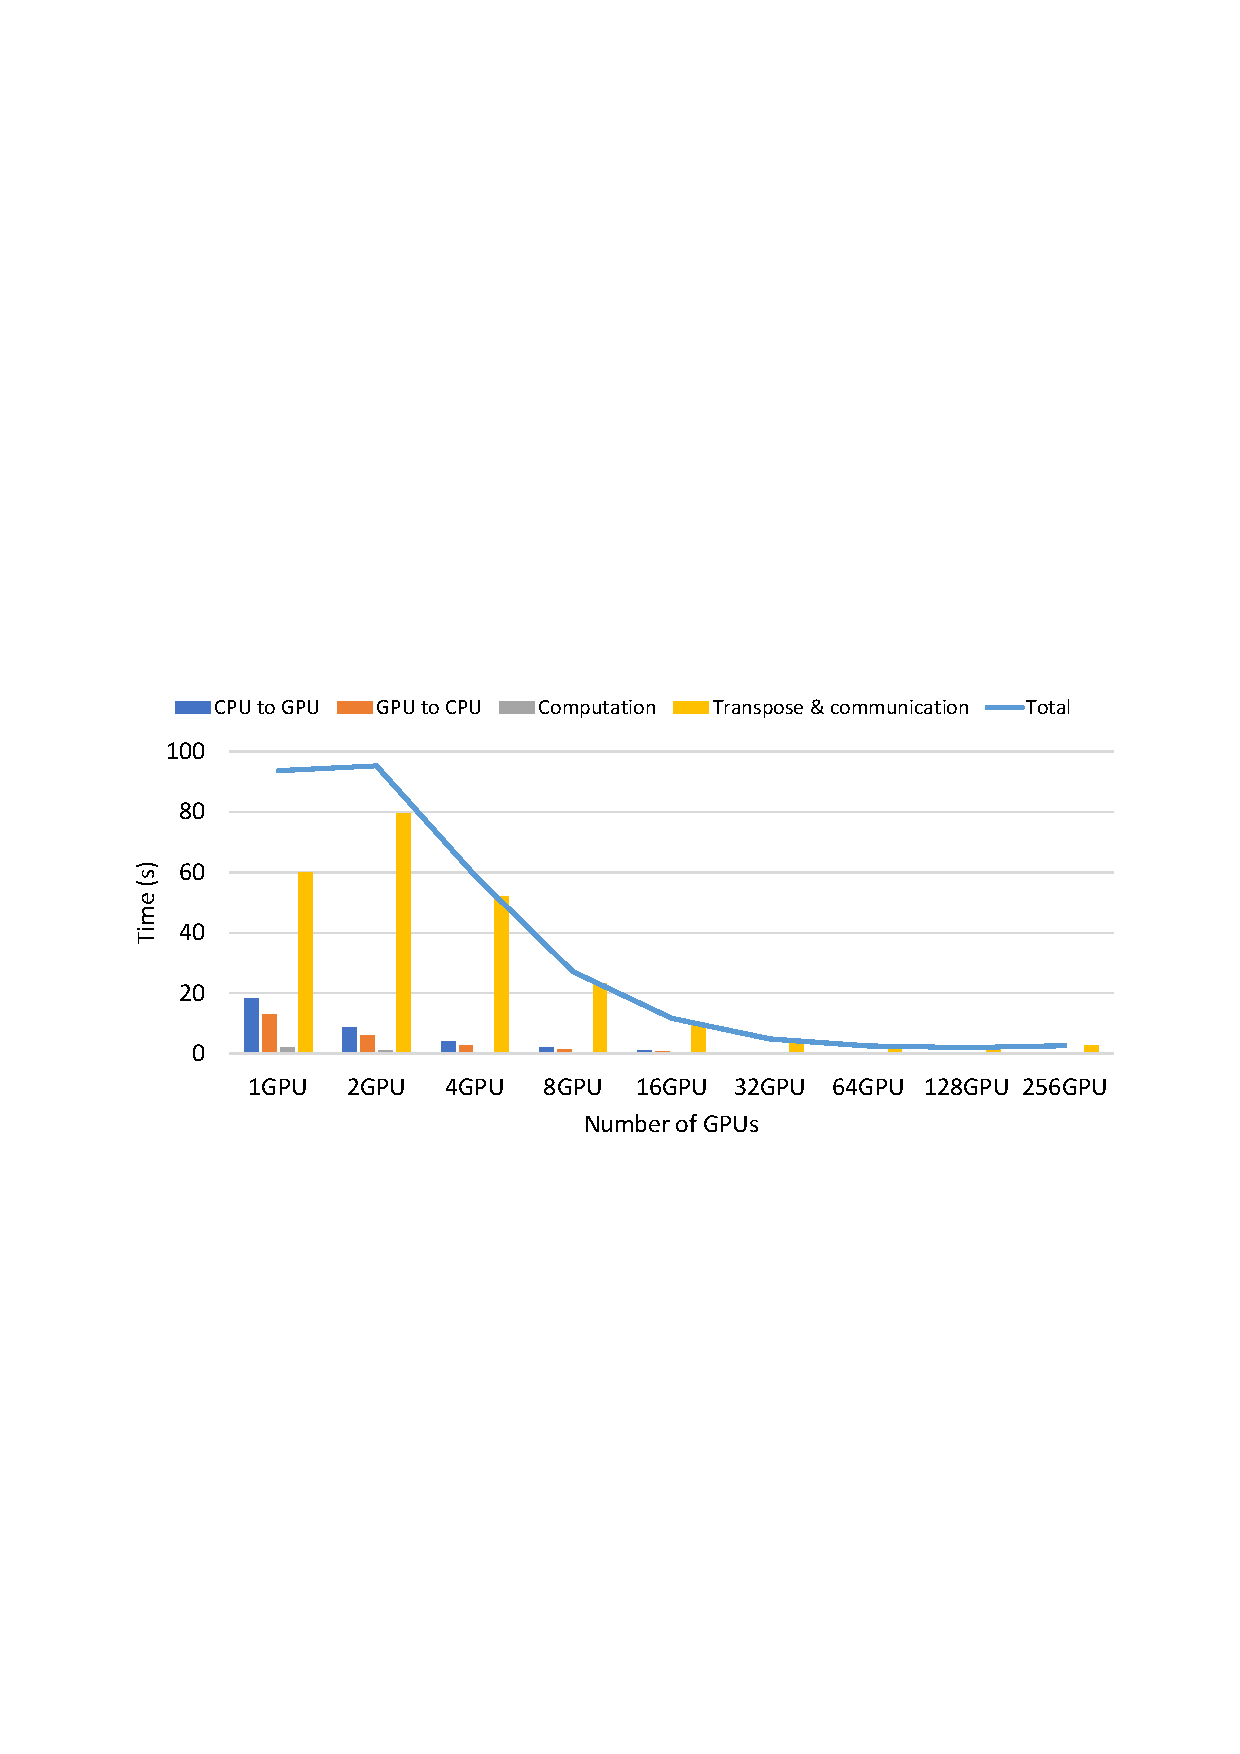
\includegraphics[width=0.9\textwidth]{Img/domain_decomposition_Titan128.pdf}} \\
  \end{tabular}
  \caption{$128 \times 128 \times 128$格点下,跨节点多~GPU~域分解模式解泊松方程时间随~GPU~个数的变化}
  \label{fig:TITAN_GPU_Poisson128}
\end{figure}

\begin{table}
  \centering
  \begin{tabular}{|>{\small}l|c|c|c|c|c|c|c|c|c|}
    \hline
    GPU数目	    &1	    &2	    &4	    &8 	    &16	    &32  	&64     &128	&256   \\
    \hline
    CPU to GPU	&18.29	&8.687	&3.946	&2.023	&0.953	&0.404	&0.148	&0.064	&0.033 \\
    GPU to CPU	&13.11	&6.15	&2.618	&1.463	&0.795	&0.368	&0.139	&0.07	&0.036 \\
    FFT计算  	&2.185	&1.034	&0.522	&0.266	&0.138	&0.071	&0.036	&0.021	&0.017 \\
    转置和通讯	&59.99	&79.34	&51.85	&23.30	&9.797	&4.041	&2.237	&1.859	&2.506 \\
    总计	    &93.58	&95.21	&58.94	&27.05	&11.68	&4.884	&2.56	&2.014	&2.592\\
    \hline
  \end{tabular}
  \caption{$128 \times 128 \times 128$格点下,跨节点多GPU域分解模式解泊松方程各部分所用时间}
  \label{tab:TITAN_GPU_Poisson128}
\end{table}

在$64 \times 64 \times 64$和$128 \times 128 \times 128$两种情况下,总时间开始都随着GPU数目增加而减小,然后到达最小值,随后由于通讯所需要的时间变大,总时间也随之变大。
\subsubsection{小结}
通过上面对于“域分解模式”的实现和测试,可以看出其主要受限于CPU和 GPU之间数据拷贝的速度与CPU和CPU之间的通讯速度。如果GPU带宽足够大,或者以后能够实现GPU与GPU之间的直接通讯的话,“域分解模式”可以作为一个可行的方案。但是在目前,与“复制模式”的比较,“域分解模式”由于其额外的数据拷贝和通讯开销,并不能通过减少运算量来达到提高速度的目的。所以我们在程序中依然使用“复制模式”,即使所有的GPU都同时运行同样的程序。

\subsection{粒子推动}
在小节\ref{section:PIC_GPU_depositor}粒子权重过程中,粒子是按照区块排列的。因此在推动粒子的时候,直接的方法是像权重过程中一样,由每个线程处理一个区块中的粒子。然而这种方法的缺陷是每个线程上的负载不均匀,可能出现某些区块中粒子数很多从而其线程运算量很大,然而另外某些区块中的粒子数较少,其线程运算量很小的情况。为了保证负载的均衡,我们采取另外一种方法,先把区块中的粒子信息重组,拷贝到一个典型的6*N的连续数组中,其中N是粒子数,6是维度;然后再并行推动。这种方法虽然需要额外的时间进行数据拷贝,但是相比第一种区块推动的负载更均匀,所以整体时间比区块推动更短,其流程如下所示:
\begin{enumerate}
  \item 将粒子从区块格式\verb"dev_ray_tile[lth*dim*npm*mth]" 重新排列,并拷贝到经典的6*N数组中\verb"dev_ray[N][6]"。
  \item 对\verb"dev_ray[N][6]"进行并行推动。
  \item 推动完成后,将粒子拷贝回原区块\verb"dev_ray_tile[lth*dim*npm*mth]" 中,以用来下一步的粒子排序和权重插值。
\end{enumerate}


\section{PIC算法在GPU上的正确性校验}
模拟程序最重要的确保模拟结果的正确性,我们通过将GPU程序的结果与成熟的CPU程序的结果进行比较来验证GPU程序的正确性。
图\ref{fig:PIC_GPU_benchmark}是CPU程序和~GPU~程序的发射度比较,从图中可以看出,两个程序得到的结果完全相同。通过输出数据得到,两者的区别在十的负十三次方量级,这可能是由于双精度浮点数的精度所限,双精度浮点数的精确度在十的负十四左右。而一般我们输出只取九位有效数字,所以可以认为两个程序的输出结果完全相同,GPU程序的正确性得到了验证。
\begin{figure}[!htb]
    \centering
    \begin{subfigure}[b]{0.9\textwidth}
        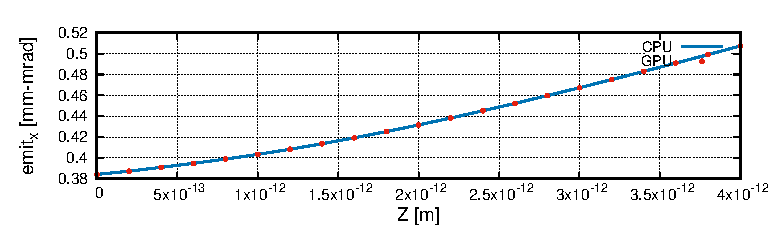
\includegraphics[width=\textwidth]{Img/PIC_GPU_benchmark_x.eps}
        %\caption{}
    \end{subfigure}
    \begin{subfigure}[b]{0.9\textwidth}
        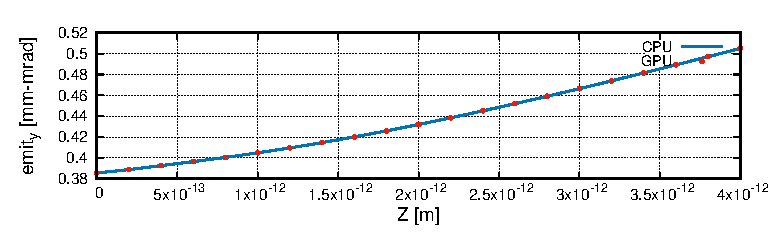
\includegraphics[width=\textwidth]{Img/PIC_GPU_benchmark_y.eps}
        %\caption{}
    \end{subfigure}
    \begin{subfigure}[b]{0.9\textwidth}
        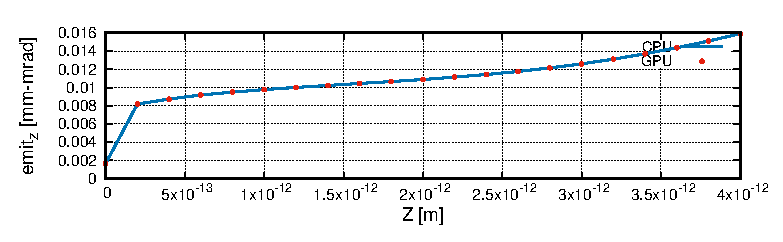
\includegraphics[width=\textwidth]{Img/PIC_GPU_benchmark_z.eps}
        %\caption{}
    \end{subfigure}
    \caption{PIC算法在GPU上的正确性校验}\label{fig:PIC_GPU_benchmark}
\end{figure}

\section{PIC算法在CPU集群上的实现}        \label{section:PIC_CPUcluster}
为了和GPU做比较,我们也在CPU集群上实现了PIC程序,其使用的计算机为Cori Knight Landing,使用的是Intel最新的众核处理器,每个处理器有68个核心。
我们的程序使用和MPI和OpenMP混合并行,以提高运行的效率。

首先,我们在一个节点上研究不同OpenMP线程数和MPI进程数下程序的效率和内存占用情况,并找到最优混合并行配置。之后,我们使用多个节点,研究程序在不同节点数下的效率变化。

\subsection{单节点}
首先,我们使用$64 \times 64 \times 64$个网格,在1.6m粒子数下测试不同的混合并行配置,如图\ref{fig:PIC_speedup_Cori_1node_1_6m}所示。其中横轴为不同的并行配置,MPI进程数由1指数增加到64,而~OpenMP~线程数有64指数得减小到1,线程数乘以进程数则保持不变。在每种并行配置下,总时间(浅蓝色实线),和权重差值,求解泊松方程,推动粒子,信息输出(各色柱行)所耗时间由左纵轴以秒为单位表示,而内存占用(绿色实线)由右纵轴以GB为单位表示。

\begin{figure}[!htb]
  \centering
  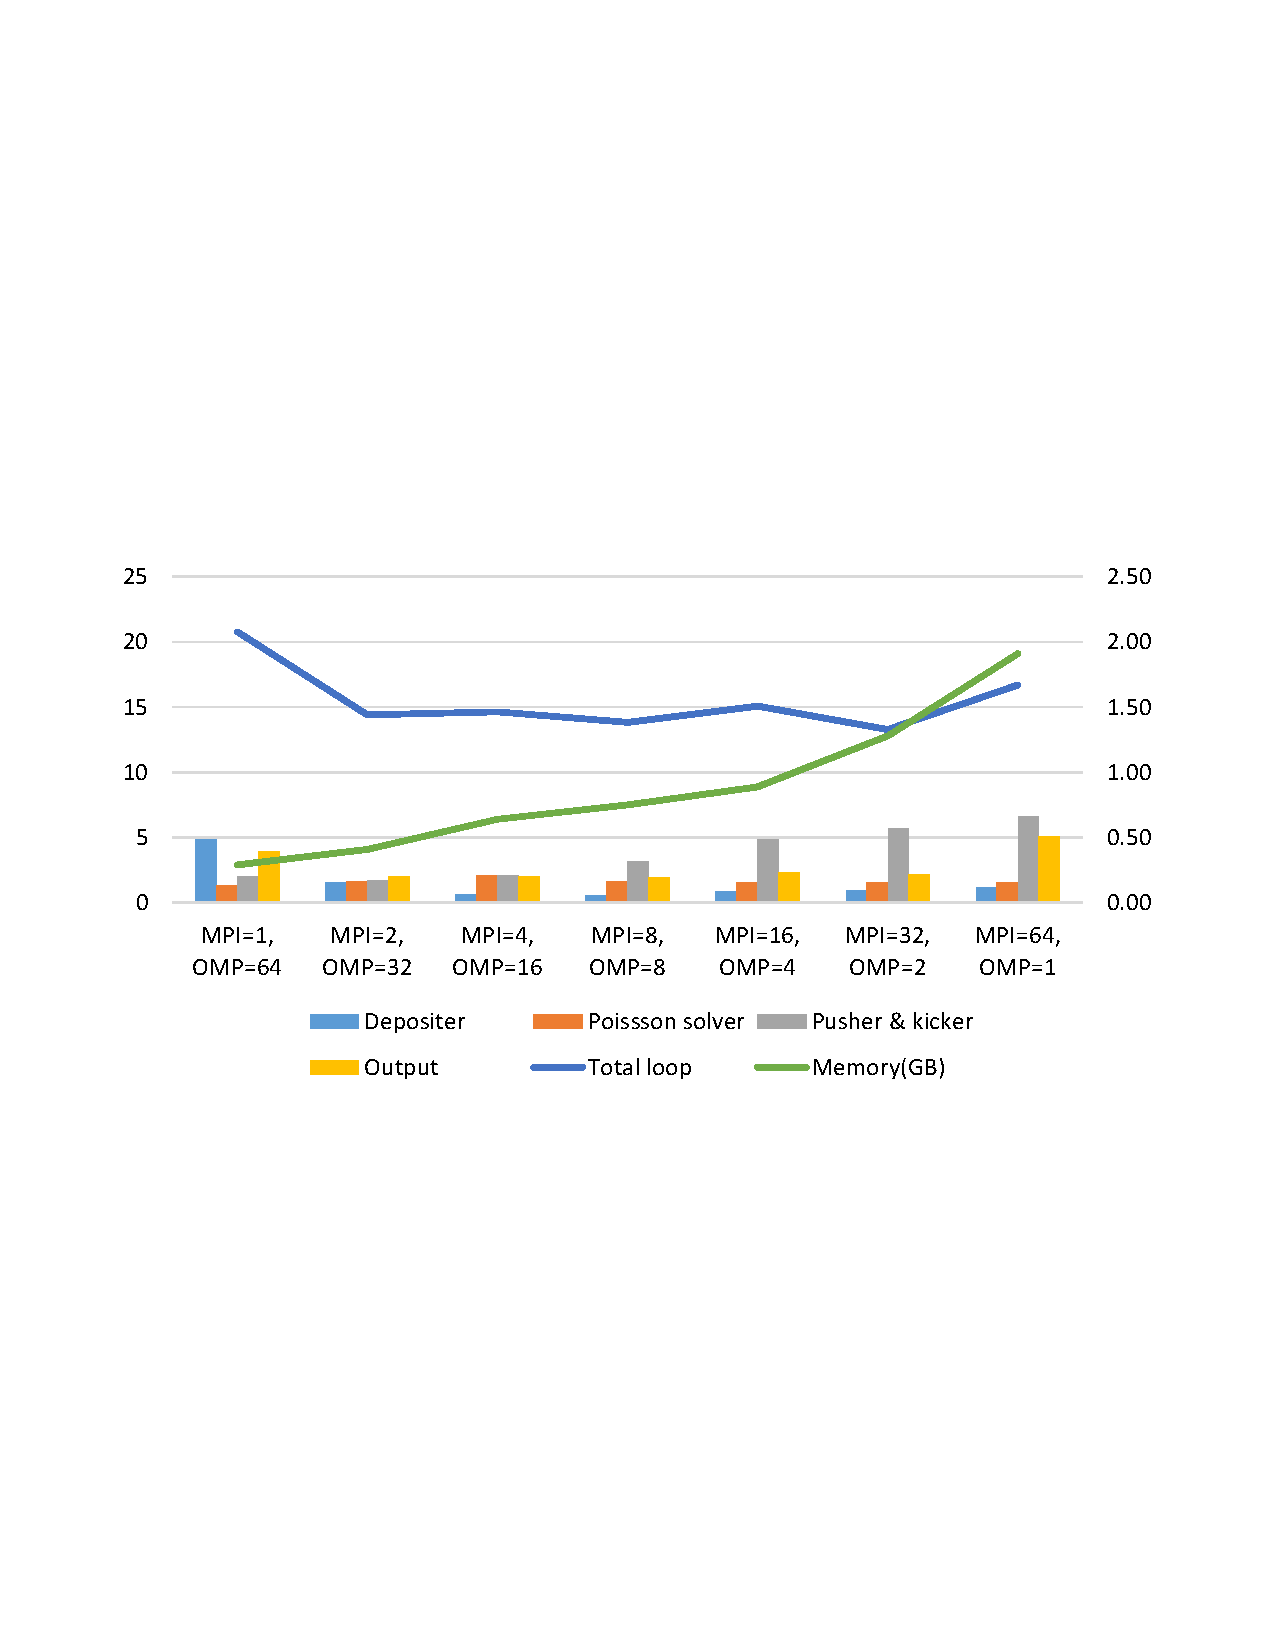
\includegraphics[width=0.9\textwidth]{Img/PIC_speedup_Cori_1node_1_6m.pdf}
  \caption{1.6m粒子数下,不同混合并行配置的耗时与内存占用}
  \label{fig:PIC_speedup_Cori_1node_1_6m}
\end{figure}

从图\ref{fig:PIC_speedup_Cori_1node_1_6m}可以看出,除了纯OpenMP并行(MPI=1,OMP=64)明显较慢外,其他各个并行配置下所消耗的总时间的差别并不大,
其中耗时最小的并行配置为使用32个MPI进程,每个进程使用2个OpenMP线程。一般而言,使用较大的MPI进程数是比较有效率的选择。
而内存占用基本随着MPI进程数目线性增加。



程序的不同部分对于并行配置的反应并不相同。随着MPI进程数的增加和每个进程所用线程数的减小,权重差值的耗时先减小后增加,一开始先从MPI=64,OMP=1时的1.14秒减少到了MPI = 8,OMP =8时的0.58秒,然后其开始剧烈增加,最终到达MPI = 1,OMP =64时的4.85秒。其原因是权重差值需要在不同的线程之间进行归约以避免线程冲突,而归约操作在线程数很大时有一个较大的启动时间。粒子推动耗时随着MPI数变大单调增加,这是因为OpenMP更适合Knight Landing众核架构,并能更有效的利用矢量处理器。

我们也测试了不同的粒子数下的并行配置,测试的粒子数为160k和16m,分别是之前粒子数的十分之一和十倍,其结果如图\ref{fig:PIC_speedup_Cori_1node_160k}和图\ref{fig:PIC_speedup_Cori_1node_16m}所示。
在160k个粒子的情况下,总时间随着MPI进程数的增加单调减少,这表明小粒子数情况更适合纯MPI并行。
而在1.6m个粒子的情况下,纯OpenMP并行由于无MPI进程间通讯,显示出一些优势,但是其总耗时依然大于MPI并行,其耗时最小的配置为MPI=64,OMP=1。

\begin{figure}[!htb]
  \centering
  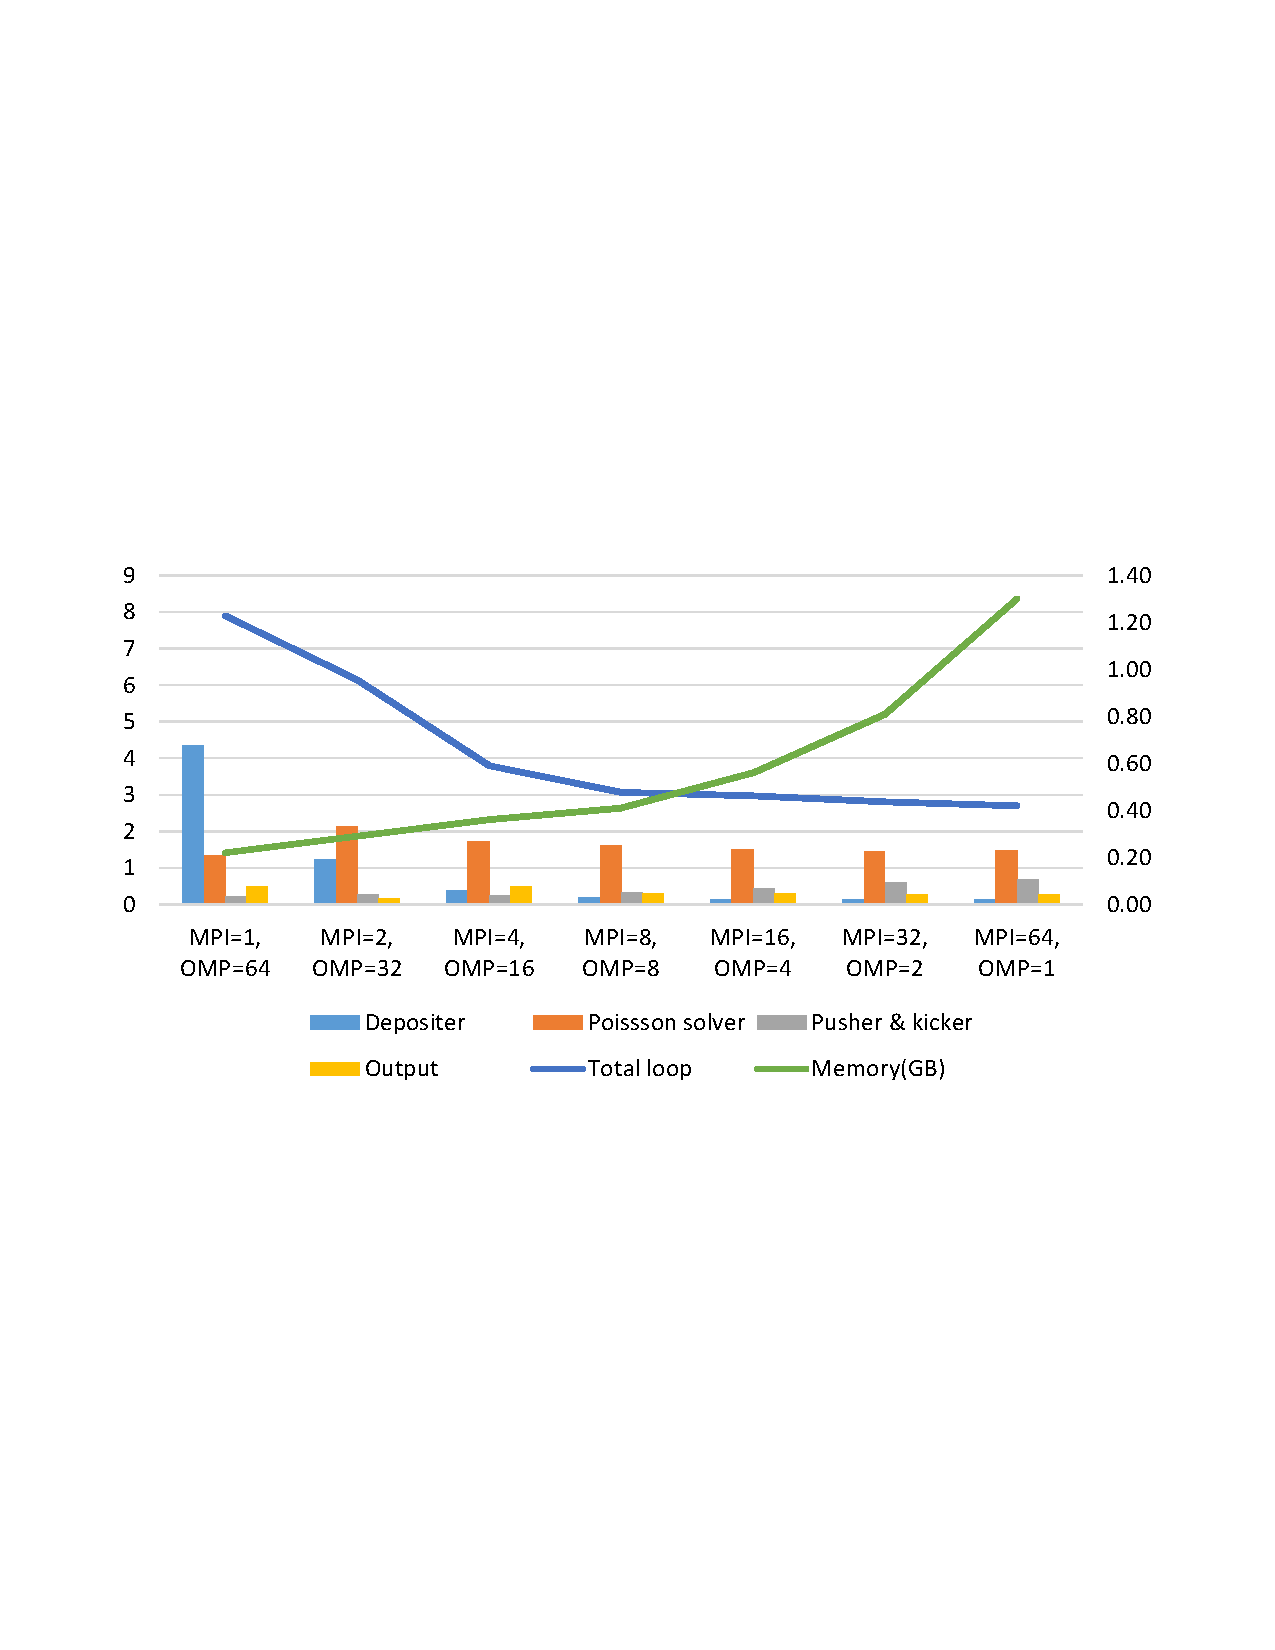
\includegraphics[width=0.9\textwidth]{Img/PIC_speedup_Cori_1node_160k.pdf}
  \caption{160k粒子数下,不同混合并行配置的耗时与内存占用}
  \label{fig:PIC_speedup_Cori_1node_160k}
\end{figure}

\begin{figure}[!htb]
  \centering
  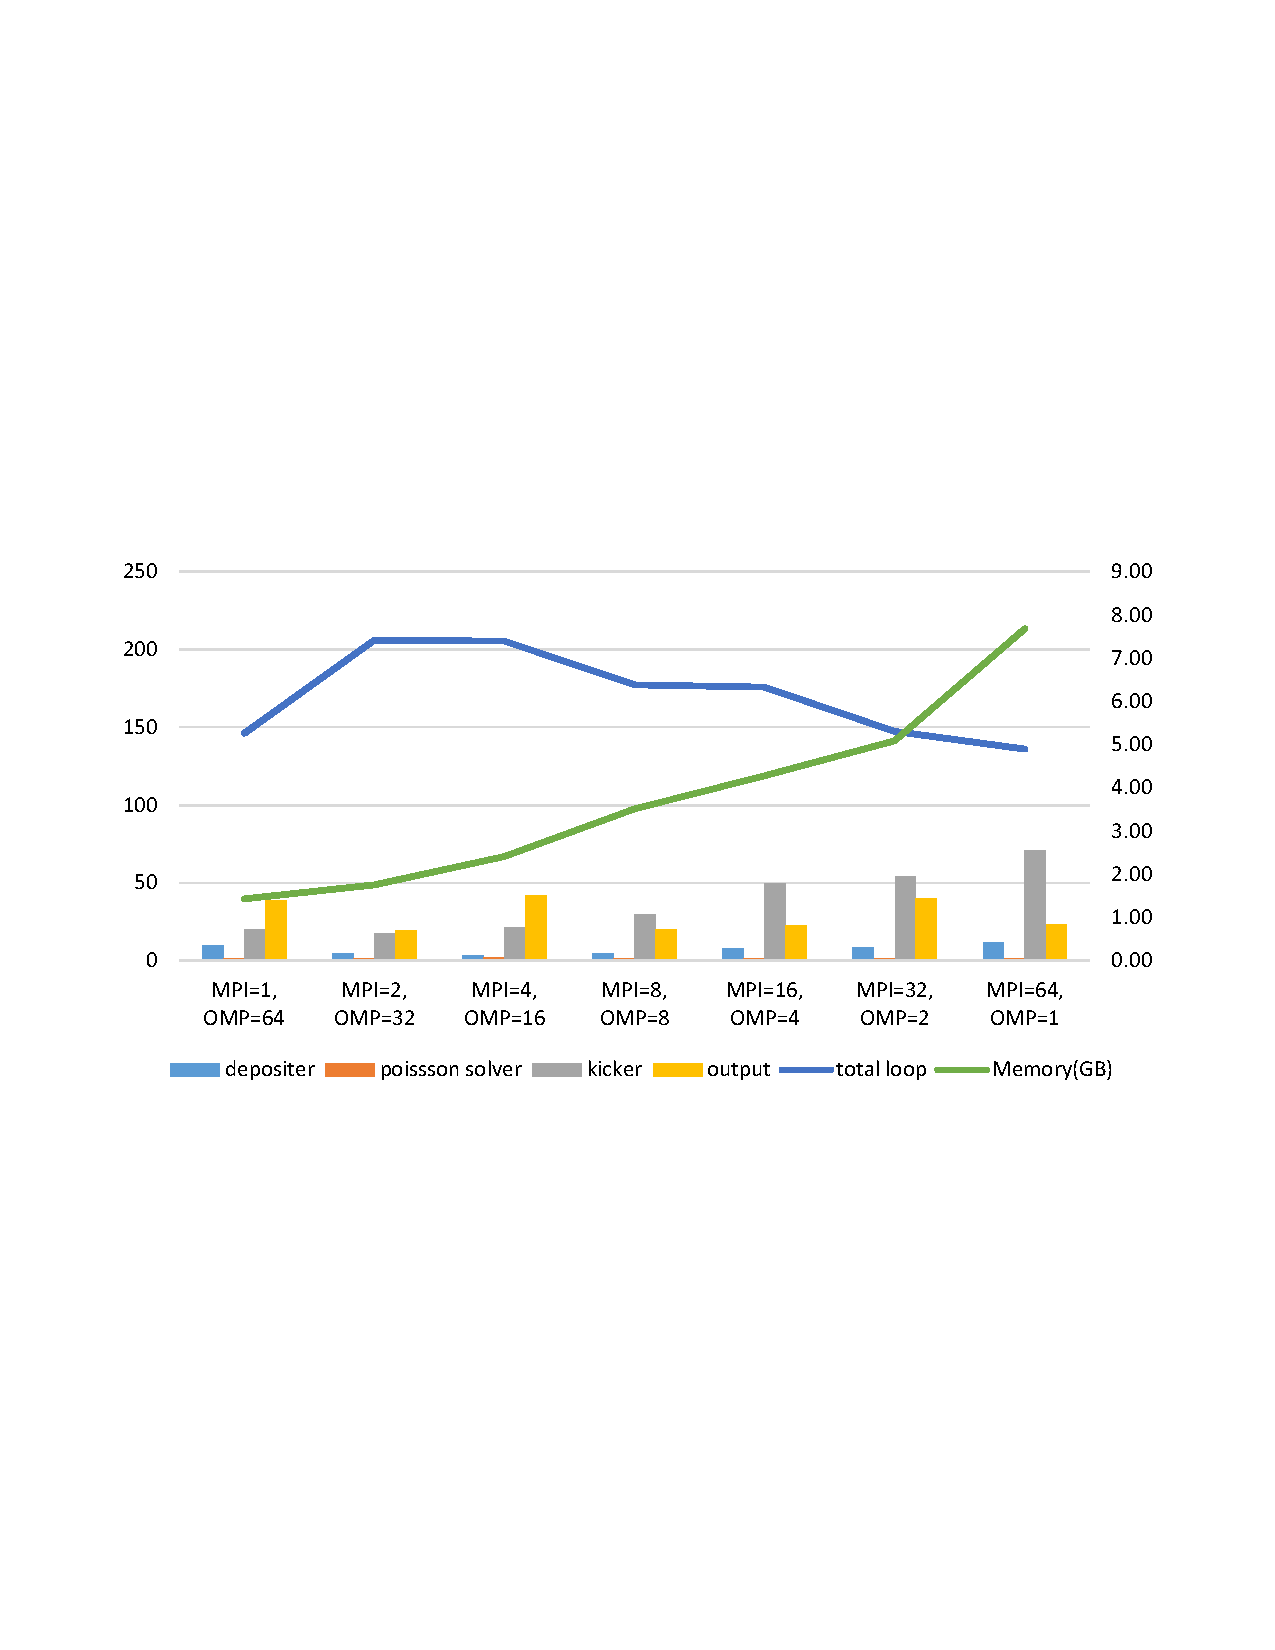
\includegraphics[width=0.9\textwidth]{Img/PIC_speedup_Cori_1node_16m.pdf}
  \caption{16m粒子数下,不同混合并行配置的耗时与内存占用}
  \label{fig:PIC_speedup_Cori_1node_16m}
\end{figure}

在各种情况下,无论粒子数多少,内存占用总是随着MPI进程数变大而单调增加。
\subsection{多节点}
从上面单节点的测试中可以得到,使用较大的MPI进程数和较小的OpenMP 线程数是更有效率的并行配置。
因此在多节点的测试中,我们首先选用纯MPI并行,测试在不同的节点数下程序总体以及各个部分的耗时情况。之后,我们也测试了OMP=2和OMP=4的情况,并与纯MPI程序进行了比较。

图\ref{fig:PIC_speedup_Cori_scalability}是纯MPI配置下PIC程序在CPU集群多节点下的耗时情况。每个节点我们使用64个核,图\ref{fig:PIC_speedup_Cori_scalability}的横轴为节点数目;左纵轴为时间,以秒为单位;右纵轴为内存使用,以GB为单位。随着使用更多的节点,程序总耗时先降低后增加,在32个节点处到达最小值。总耗时先减小是因为使用的节点数越多,每个节点上需要进行的运算越少;后增加是因为随着节点数上升,节点间的通讯时间也会随之增加。图\ref{fig:PIC_speedup_Cori_percetage_64nodes}为使用64个节点时程序各个部分消耗时间所占的百分比,可以看出此时通讯耗时已经占了总耗时的60\%。

\begin{figure}[!htb]
  \centering
  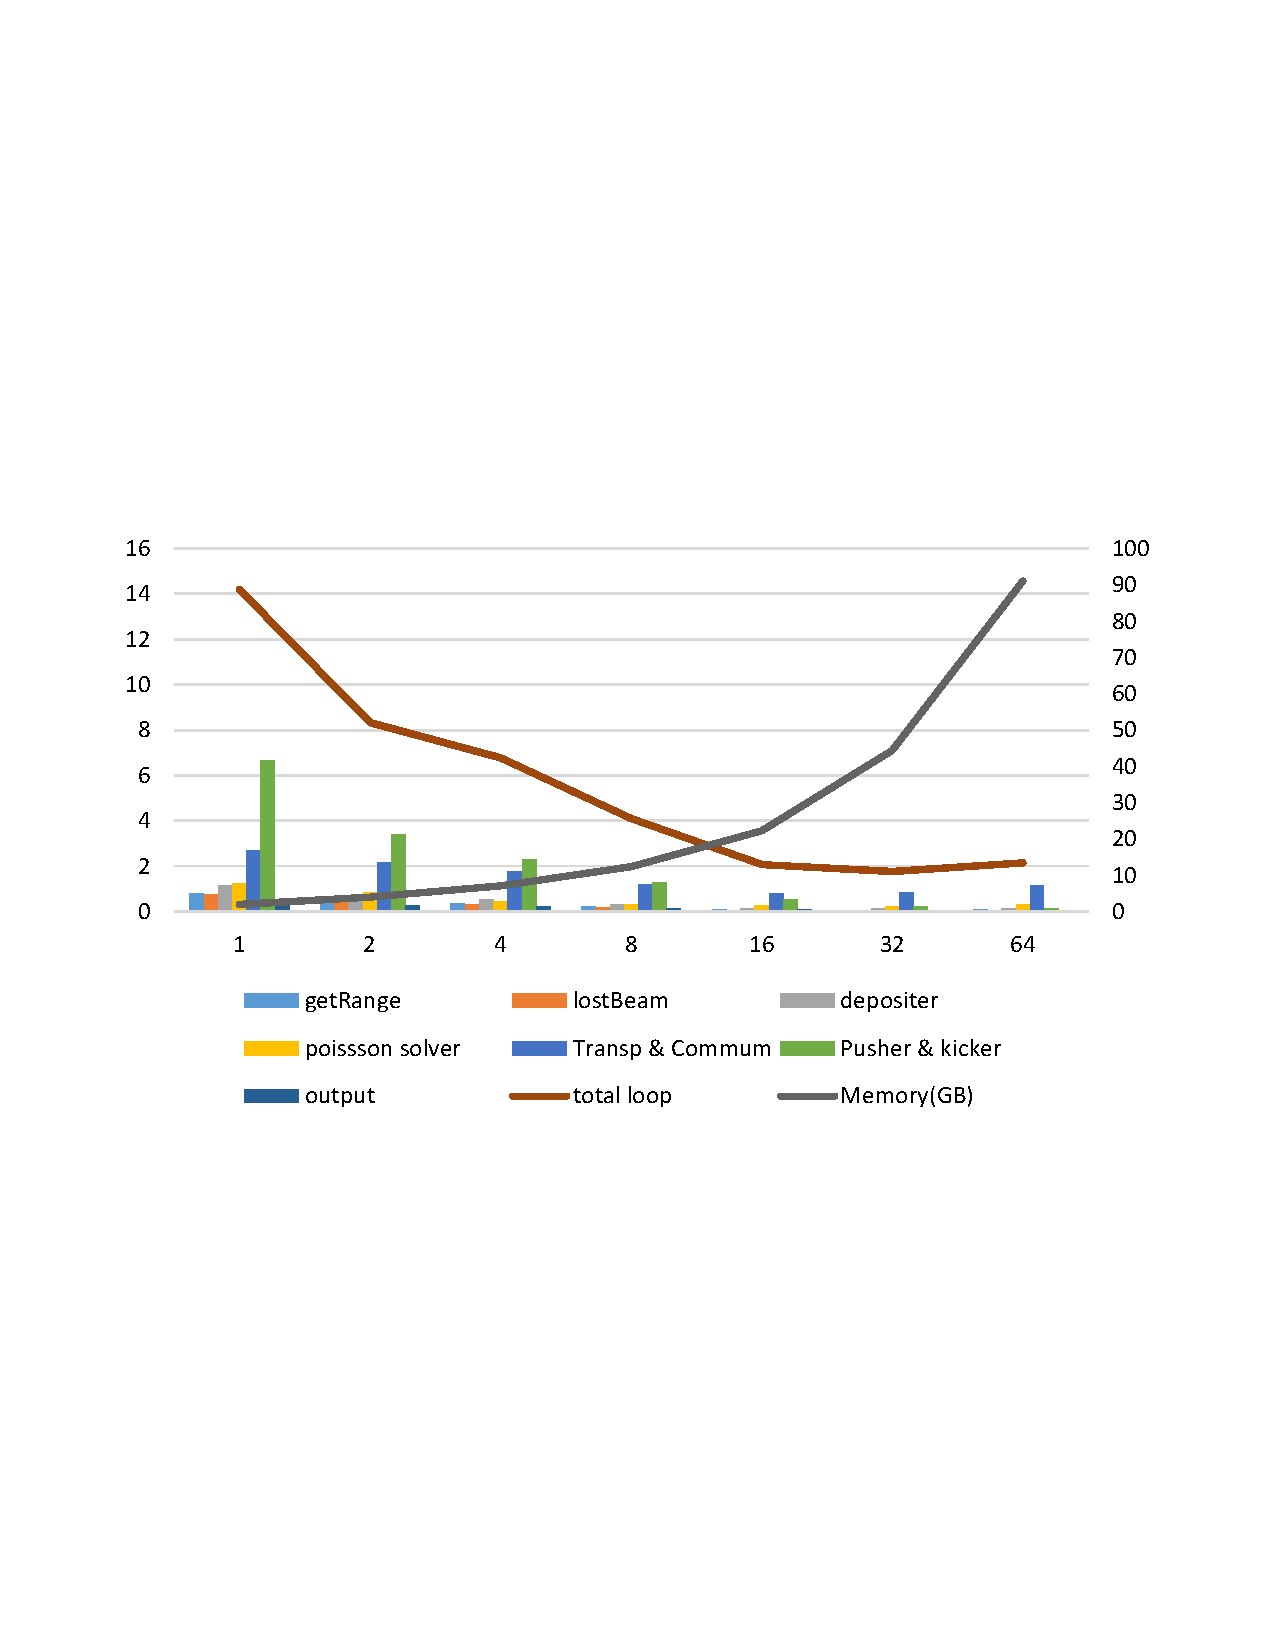
\includegraphics[width=0.9\textwidth]{Img/PIC_speedup_Cori_scalability.pdf}
  \caption{PIC程序使用多个CPU节点的耗时}
  \label{fig:PIC_speedup_Cori_scalability}
\end{figure}

\begin{figure}[!htb]
  \centering
  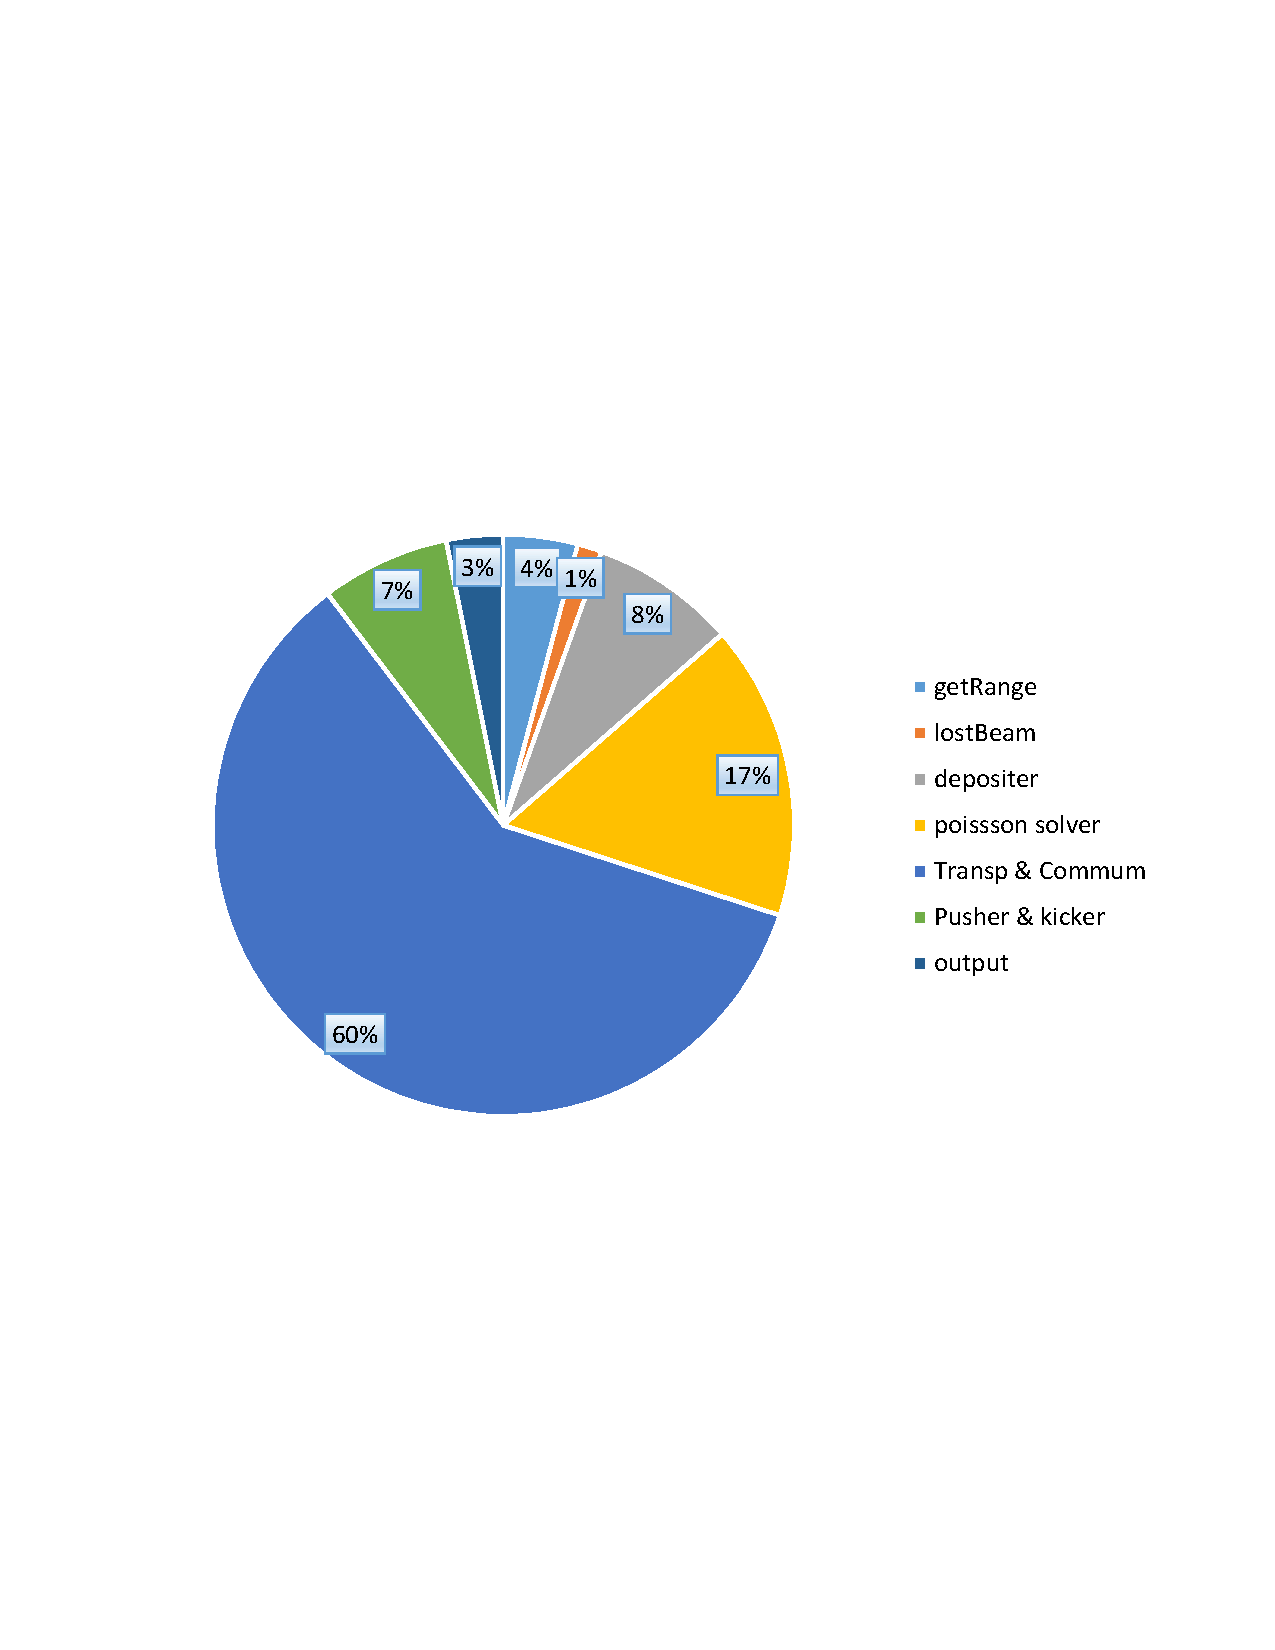
\includegraphics[width=0.5\textwidth]{Img/PIC_speedup_Cori_percetage_64nodes.pdf}
  \caption{使用64个节点时程序各个部分消耗时间所占的百分比}
  \label{fig:PIC_speedup_Cori_percetage_64nodes}
\end{figure}

接下来,我们对OMP=2和OMP=4的并行配置进行了测试,并与纯MPI程序(OMP=1)进行了比较,如图\ref{fig:PIC_speedup_Cori_multi_nodes_timeMemory}所示。
在大部分情况下,不同并行的耗时差别很小;但是在某些情况下差别很大,比如节点数为16时,纯MPI的速度是OMP=4的 1.8倍。
对于内存使用情况, 使用更多的OpenMP线程和更少的MPI进程总是占优势。
综合考虑,在内存足够大的情况下,在Knight Landing上运行的PIC程序使用纯MPI并行配置依然是一个很好的选择。

\begin{figure}[!htb]
    \centering
    \begin{subfigure}[b]{0.48\textwidth}
        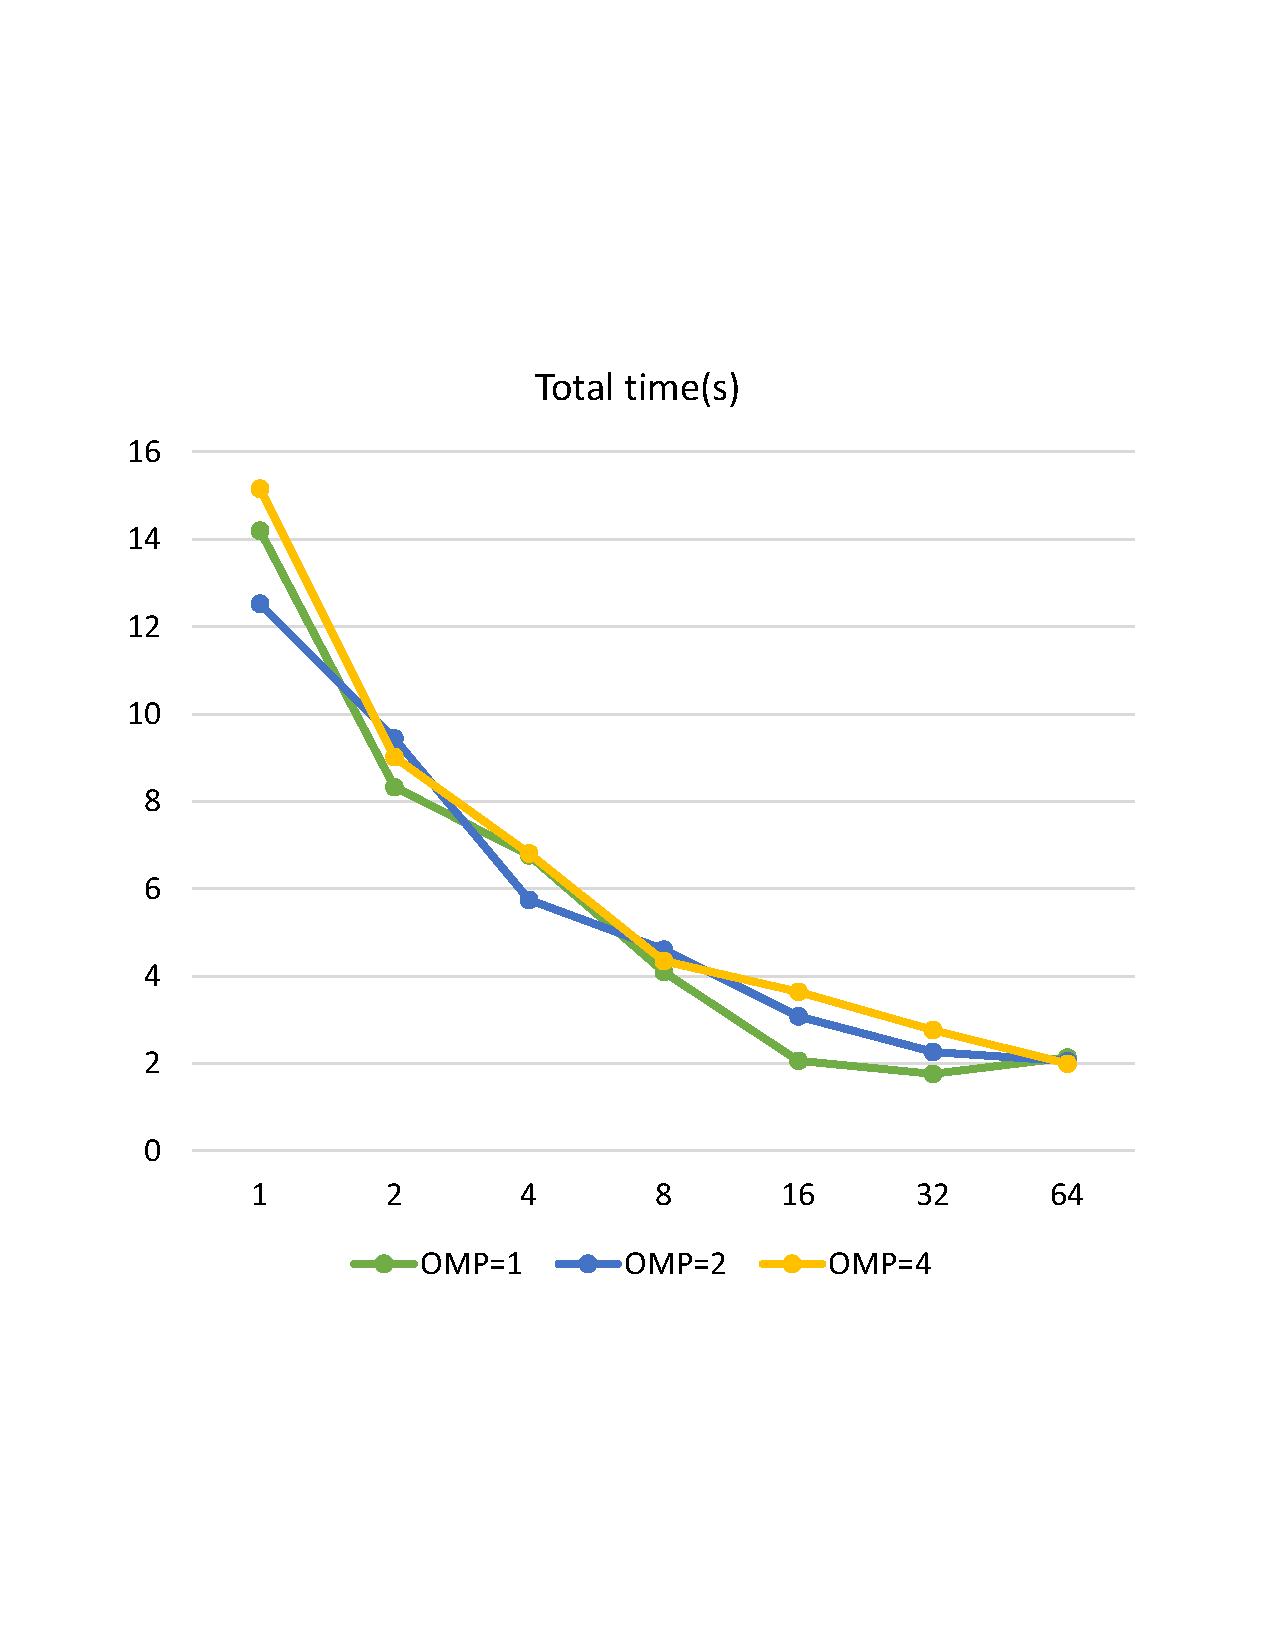
\includegraphics[width=\textwidth]{Img/PIC_speedup_Cori_multi_nodes_time.pdf}
        \caption{耗时}
    \end{subfigure}
    \begin{subfigure}[b]{0.48\textwidth}
        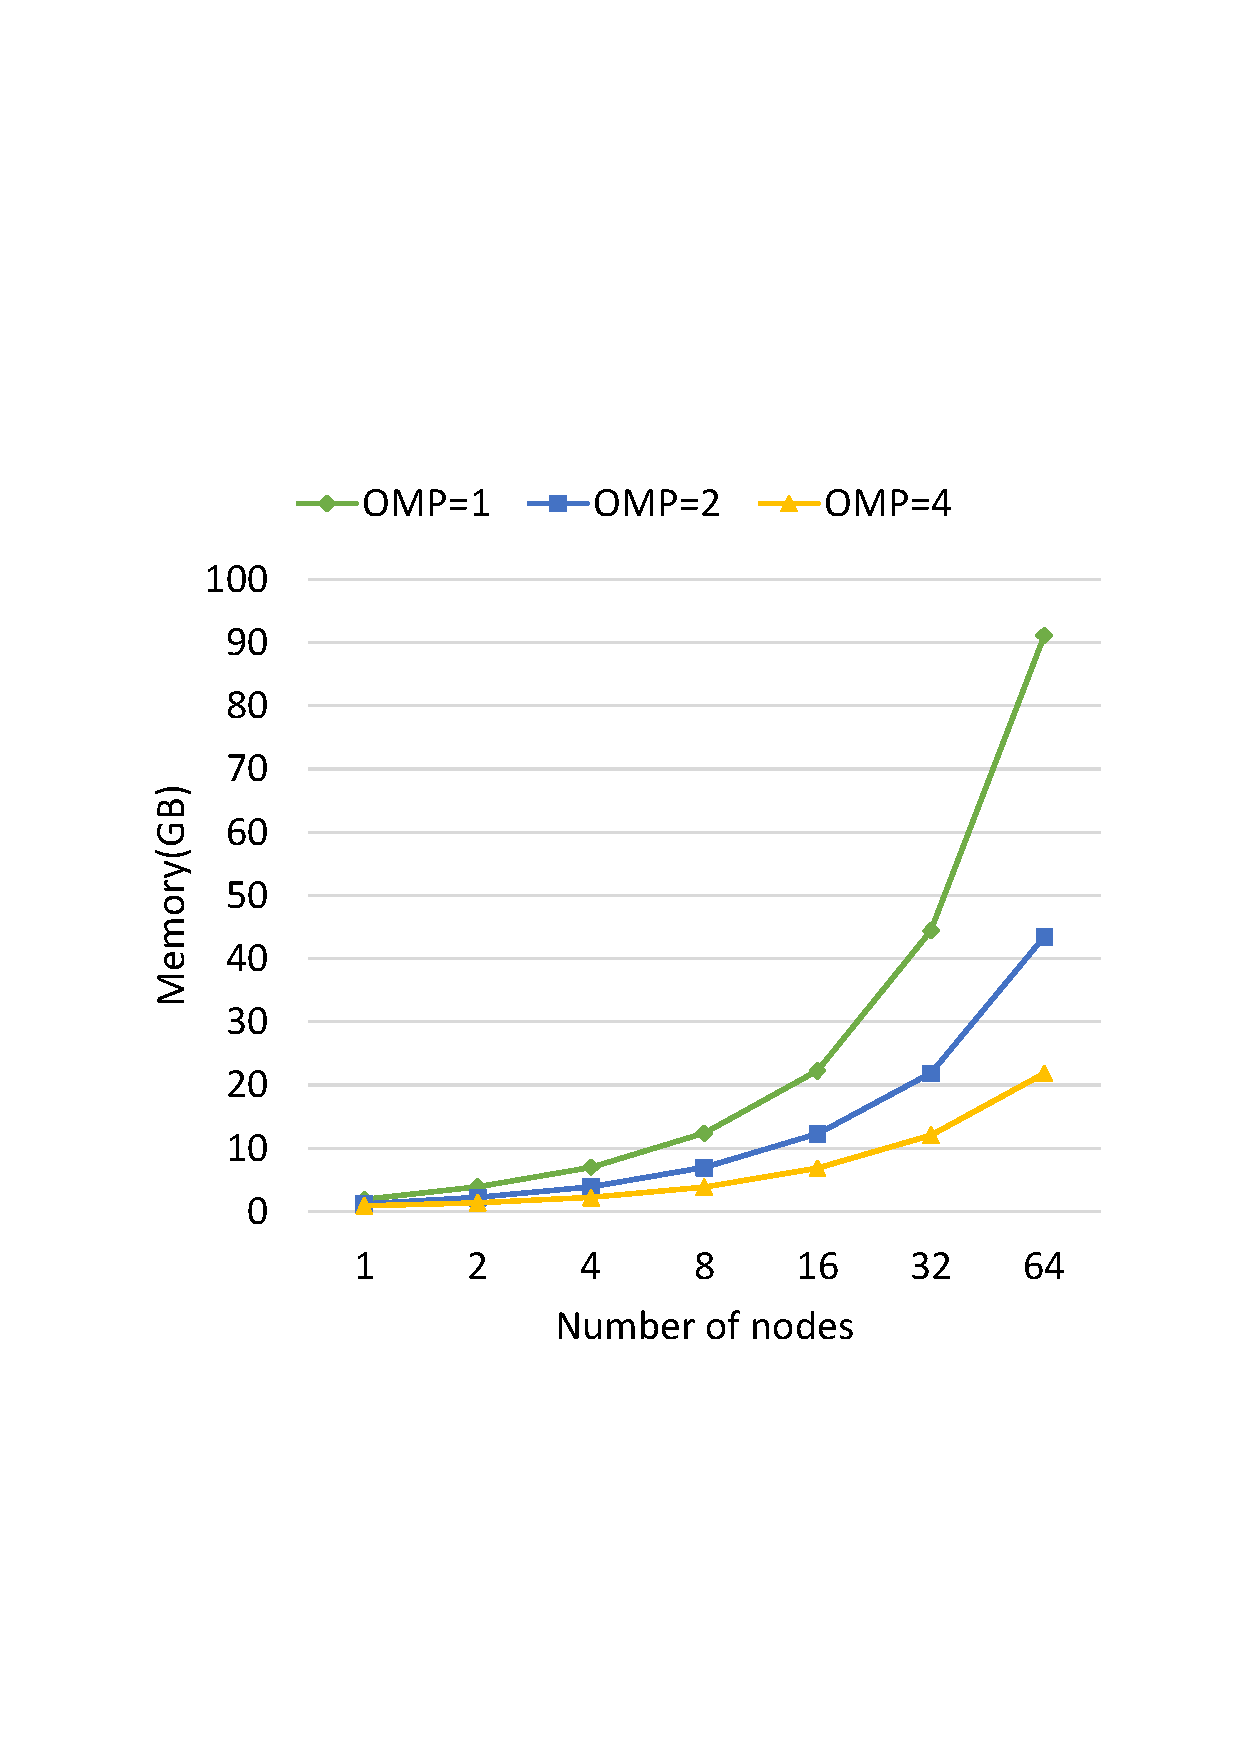
\includegraphics[width=\textwidth]{Img/PIC_speedup_Cori_multi_nodes_memory.pdf}
        \caption{内存占用}
    \end{subfigure}
    \caption{不同并行配置下的多节点运行情况比较}
    \label{fig:PIC_speedup_Cori_multi_nodes_timeMemory}
\end{figure}

\subsection{与GPU对比}

在本章之前的测试中,我们使用的GPU型号为Nvidia GeForce GTX 1060,其包含1280颗核心,时钟频率为1.71GHz。而我们使用的CPU型号为Intel® Xeon Phi™ Processor 7250 ("Knights Landing"),共包含68颗核心,时钟频率为1.40GHz,但是实际上,我们只是使用了64颗核心。

而由于GPU程序做了一些简化,缺少一部分步骤,例如粒子丢失判据等,我们在进行比较的时候也在CPU程序的耗时中减去了相应部分。
在$64 \times 64 \times 64$个格点数,1.6m个粒子的情况下,对于同样长度的加速器,使用一个GPU代码的总耗时为3.56秒,这类似于CPU程序在300个核心上的运行时间。换而言之,对于我们的PIC程序,一个GPU卡的运算效率与4到8个CPU节点的运行效率相当。


\section{Symplectic算法在GPU上的实现}     \label{section:symplectic_GPU}
Symplectic算法非常适合使用GPU进行加速计算。通过使用CUDA和GPU,可以显著加快无网格粒子跟踪代码的运行速度。当运行在单个GTX 1060时,与CPU串行相比,GPU代码实现了超过400倍的加速。此外,加速比会随着GPU的数目线性增长。
在大多数加速元件中,粒子会被推动若干步。在每一步中,粒子将首先被外场传输矩阵传输推动半个时间步长,然后由空间电荷推动一个时间步长,并再次被外场传输矩阵传输推动半个时间步长。
其中,求解空间电荷将消耗整个计算时间的90%以上。 计算空间电荷效应的程序由下面的三个子程序组成,而每个子程序由一个或两个内核组成。
\begin{enumerate}
  \item 遍历三角函数
  \item 计算$\Phi^{lmn}$
  \item 计算$ep_i$并推动粒子
\end{enumerate}

我们对程序进行了许多优化,使其更适合GPU架构,程序的性能得到显着改善。 每个子程序的优化策略各不相同,下面介绍各个内核的详细优化策略。
\subsection{遍历三角函数}
根据粒子的位置,我们首先计算每个粒子的三角函数临时变量。设:
\begin{equation}
\begin{array}{cc}
    S^{l}_j =sin(\alpha_l x_j), & C^{l}_j =cos(\alpha_l x_j)  \\
    S^{m}_j =sin(\alpha_m x_j), & C^{m}_j =cos(\alpha_m x_j)  \\
    S^{n}_j =sin(\alpha_n x_j), & C^{n}_j =cos(\alpha_n x_j)  \\
\end{array}
\end{equation}
其中下标$j$是指不同的粒子,下标$l$,$m$和$n$是指三个方向的频谱模式。

然后,X方向上的传输矩阵$ m_2 $(等式\ ref {eq:map1})可以表示为:
\begin{equation}\label{eq:map2}
{{p}_{xi}}(\tau )={{p}_{xi}}(0)-\tau \frac{1}{{{\varepsilon }_{0}}}\frac{8}{abc}\omega \kappa {{\gamma }_{0}}\sum\limits_{j=1}^{{{N}_{j}}}{\sum\limits_{l=1}^{{{N}_{l}}}{\sum\limits_{m=1}^{{{N}_{m}}}{\sum\limits_{n=1}^{{{N}_{n}}}{\frac{{{\alpha }_{l}}S_{j}^{l}S_{j}^{m}S_{j}^{n}C_{i}^{l}S_{i}^{m}S_{i}^{n}}{(\alpha _{l}^{2}+\beta _{m}^{2}+\gamma _{n}^{2})}}}}}
\end{equation}

与等式\ref{eq:map1}相比,新的传输矩阵节省了很大的计算量。
计算$ S_ {j} $和$ C_ {j}$是非常有必要的,这样可以避免后期处理的重复计算。在这个子程序中,我们采用按照粒子分配线程的策略,即每个线程处理一个粒子,这段程序结构相对简单,只占整个空间电荷效应求解所需时间的2%左右。 然而,它生成了$ 2 \times({{N}_{l}} + {{N}_{m}} + {{N}_{n}})\times {{N} _ {j}} $ 的数据,占了大部分的内存空间,而GPU的内存大小在给定型号的情况下是一个固定值,并不能通过添加内存条来增加,在这个意义上,这段程序决定了模拟中粒子数目的最大值,是花费存储空间以节省计算量而的典型示例。根据我们的测试,考虑到不可避免的内存碎片,假设展开阶数为$64\times64\times64$,程序可以在GeForce GTX 1060 6GB上处理大约100万个粒子。

由于需要遍历内存,该子程序的速度受到全局内存带宽的限制。为了改进内存读写,粒子数据是以阵列结构(SoA)排列的形式而不是结构数组(AoS),以达到对齐读取(coalesced memory read)。并且,在CPU侧分配页锁存存储器,以实现 CPU与GPU之间的数据复制速度更快。

\subsection{计算$\Phi^{lmn}$}\label{section:phi}
我们注意到在传输矩阵\ref{eq:map2}中,对下标$j$的求和是对每个粒子的求和,我们可以改变求和的顺序以节省计算量。如果我们定义:
\begin{equation}
\Phi^{lmn}\equiv \sum\limits_{j=1}^{{{N}_{j}}}{S_{j}^{l}S_{j}^{m}S_{j}^{n}}
\end{equation}

如果首先完成${{N}_{l}}\times{{N}_{m}}\times{{N}_{n}}$个$\Phi^{lmn}$的计算。传输矩阵\ref{eq:map2}可以重写为:

\begin{equation}\label{eq:map3}
{{p}_{xi}}(\tau )={{p}_{xi}}(0)-\tau \frac{1}{{{\varepsilon }_{0}}}\frac{8}{abc}\omega \kappa {{\gamma }_{0}}\sum\limits_{l=1}^{{{N}_{l}}}{\sum\limits_{m=1}^{{{N}_{m}}}{\sum\limits_{n=1}^{{{N}_{n}}}{\frac{\Phi^{lmn}{{\alpha }_{l}}C_{i}^{l}S_{i}^{m}S_{i}^{n}}{(\alpha _{l}^{2}+\beta _{m}^{2}+\gamma _{n}^{2})}}}}
\end{equation}

以这种方式,计算复杂度从$\alpha N_p^2*N_{modes}$减少到了$\alpha  N_p*N_{modes}$,这使这个保辛粒子跟踪算法的计算量大大降低。

该子程序的目的是为每个展开模计算$\Phi^{lmn}$,自然地我们使用每个线程处理一个模的方式。
然而,在通常情况下,我们使用$16\times 16\times 16$模式就可以得到收敛的结果,也就是说会有$16\times 16\times 16 = 4096$个线程,而GPU通常具有几百甚至几千个核心,这个线程数量相对于的GPU的核心数目来说较少。
为了实现负载平衡,我们将粒子分为几个部分,并采用CUDA流技术来获得高并发性。我们定义临时变量$\Phi^{lmn}_{temp,i}$:
\begin{equation}
\Phi^{lmn}_{temp,i}\equiv \sum\limits_{j=Nstar{{t}_{i}}}^{Nen{{d}_{i}}}{S_{j}^{l}S_{j}^{m}S_{j}^{n}}
\end{equation}
那么,$\Phi^{lmn}$由以下求和得到:
\begin{equation}
\Phi^{lmn}=\sum\limits_{i}{\Phi^{lmn}_{temp,i}}
\end{equation}

这个子程序的速度也是受到内存带宽的限制。我们在计算$Phi^{lmn}$之前,会首先对$S_{j}$进行转置以达到对齐读取。

\subsection{计算$ep_i$并推动粒子}
以x方向为例,我们定义:
\begin{equation}
ep{_{xi}}\equiv \tau \frac{1}{{{\varepsilon }_{0}}}\frac{8}{abc}\omega \kappa {{\gamma }_{0}}\sum\limits_{l=1}^{{{N}_{l}}}{\sum\limits_{m=1}^{{{N}_{m}}}{\sum\limits_{n=1}^{{{N}_{n}}}{\frac{\Phi^{lmn}{{\alpha }_{l}}C_{i}^{l}S_{i}^{m}S_{i}^{n}}{(\alpha _{l}^{2}+\beta _{m}^{2}+\gamma _{n}^{2})}}}}
\end{equation}

我们首先根据前两个小节中得到的$\Phi^{lmn}$, $S_{j}^{{}}$和$C_{j}^{{}}$计算得到$ep{_{xi}}$,随后,使用~$ep{_{xi}}$~对粒子进行推动。传输矩阵\ref{eq:map3}可以重新写为一个简洁的形式:
\begin{equation}\label{eq:map4}
{{p}_{xi}}(\tau )={{p}_{xi}}(0)-ep{_{xi}}
\end{equation}

由于GPU寄存器数量的限制,$ep_{i}$的计算和粒子的推动在X,Y,Z三个方向上分别进行,以提高GPU占用率和运算效率。在这个子程序中,内层最内层循环会以不同的顺序访问$Phi^{lmn}$,所以在调用此子例程,我们需要对$ Phi ^ {lmn} $进行转置,以实现对齐读取,提高效率。

在个方向上,我们根据粒子来分配线程。这段程序受到GPU常量内存大小和GPU共享内存大小的限制有两个分支:一个是在阶数小于$20 \times 20 \times 20$的情况下,另一种是阶数大于$20 \times 20 \times 20$的情况。
\subsubsection{分支1:阶数小于$20 \times 20 \times 20$}
当阶数小于$ 20\times20\times20 $时,我们使用常量内存保存$Phi^{lmn}$。常量内存是专门针对广播进行优化的,即多个线程同时访问同一常量内存地址的速度很快,正适合需要被每个线程访问的$Phi^{lmn}$。一个普通GPU中的常量内存总量为65536字节,只能容纳8192个双精度浮点数。正是这个常量内存的大小,决定了小于$20 \times 20 \times 20$和大于$20 \times 20 \times 20$两个分支的分界点。

在这个分支中,每个方向的内核使用共享内存存储最内部的循环中$ S_ {j} $和$ C_ {j} $。共享内存是一种片上内存,内存大小较小,每个GPU的每个流处理器只有64kb,但是共享内存的速度远远快于全局内存。由共享内存大小限制,这段程序的GPU占用率仅为25%,但是共享内存的访问延迟要比全局内存低大约100倍。

还进行了一次测试来评估使用全局内存而不是共享内存的速度。在这个测试中,我们通过数据结构的设计来使让warp中的所有线程访问连续的内存地址,尽量避免全局内存的访问延迟。由于不再受共享内存大小的限制,GPU占用率可以达到接近100%。然而,由于全局内存访问过于频繁,程序运行花费的时间接近使用共享内存程序的两倍。

\subsubsection{分支1:阶数大于$20 \times 20 \times 20$}
当阶数大于$20 \times 20 \times 20$时,受限于共享内存和常量内存的大小,上述直接计算$ep_ {i}$并推动粒子的的方式将无法有效工作,我们必须进行改变。

首先,$\Phi^{lmn}$被存储在全局内存中。在这段程序中多个线程会访问相同内存地址,而由于GPU全局内存的合并读取机制,使用全局内存的速度只比使用常量内存的速度慢10%。
另外,受限于共享内存的大小,我们将$ ep_{i} $的计算和推送粒子分开。而在$ ep_{i} $的计算中,不同的阶被分为若干部分来,分别使用共享内存。它类似于小节 \ref{section:phi}中对$\Phi^{lmn}$的计算。每个粒子会使用若干线程,而每个线程处理相应的阶,并获得临时变量${e{{p}_{i}}^{temp,j}}$。
\begin{equation}
{e{{p}_{i}}^{temp,j}}\equiv \tau \frac{1}{{{\varepsilon }_{0}}}\frac{8}{abc}\omega \kappa {{\gamma }_{0}}\sum\limits_{l=1}^{{{N}_{l}}}{\sum\limits_{m=1}^{{{N}_{m}}}{\sum\limits_{n=Nstar{{t}_{j}}}^{Nen{{d}_{j}}}{\frac{\Phi^{lmn}{{\alpha }_{l}}C_{i}^{l}S_{i}^{m}S_{i}^{n}}{(\alpha _{l}^{2}+\beta _{m}^{2}+\gamma _{n}^{2})}}}}
\end{equation}
然后我们队 ${e{{p}_{i}}^{temp,j}}$求和并根据等式\ref{eq:map4}推动粒子:
\begin{equation}
e{{p}_{i}}=\sum\limits_{j}{e{{p}_{i}}^{temp,j}}
\end{equation}
分成若干部分分别计算也有相应的缺点,分开计算需要更多的内存空间来保存~${e{{p}_{i}}^{temp,j}}$。额外的内存使用量与粒子数和阶数成正比。在相同的的内存大小分别计算的最大粒子数会比直接计算的减少约为20%。

\section{小结}                            \label{section:Code_conclusion}
本章介绍了根据PIC算法编写的粒子模拟程序P-TOPO,主要处理强流加速器中的非线性效应。
P-TOPO的PIC部分和整体正确性都得到了验证。
在GPU上,我们使用CUDA库实现了基于PIC方法的多粒子模拟程序,并优化了GPU代码结构,使用特定的并行策略避免了线程竞争,是程序的性能得以提高。
我们也新的CPU架构Cori Knight Landing上实现了PIC程序,并探索了其最佳性能的并行线程配置。通过比较,单GPU运行的程序和使用4或8个节点的程序性能相当。
我们使用CUDA库在GPU上实现了Symplectic算法。由于其算法结构非常适合使用GPU进行加速计算,程序总体加速比接近500。

\chapter{束流模拟程序的优化和性能测试} \label{chap:Performance}
随着加速器束流流强的增大,为了对束流进行精确的模拟和研究,我们需要模拟的粒子数目增加了几个量级。
在这种趋势下,束流模拟软件的效率至关重要。
本文之前在第\ref{chap:Code}章介绍了束流模拟程序在GPU和CPU上的并行实现,
接下来在本章中,首先小节\ref{section:PIC_performance}将对PIC算法在多种计算平台的性能测试进行介绍。
之后,第 \ref{section:Symplectic_performance}节将对Symplectic算法的GPU并行性能进行了测试。

\section{PIC程序性能}             \label{section:PIC_performance}
我们使用了多种计算平台对并行PIC程序的性能进行调优和测试~\cite{tiwari2015Titan,wells2016Summit,he2018Cori}:
\begin{itemize}
  \item 单GPU - GTX1060
  \item GPU集群 - Titan
  \item GPU集群 - SummitDev
  \item CPU集群 - Cori Knight Landing
\end{itemize}

Titan是一台GPU/CPU混合架构的超级计算机,位于美国橡树岭国家实验室(ORNL),
它使用的是由NVIDIA提供的Tesla计算卡和AMD提供的Opteron处理器~\cite{TitanURL}。
SummitDev是同样位于ORNL,是下一代超级计算机Summit的早期测试平台,每个SummitDev节点都有2个IBM POWER8 CPU和4个NVIDIA Tesla P100 GPU~\cite{SummitURL}。
Cori Knight Landing(KNL)是Cori的新计算平台,位于美国国家能源研究科学计算中心(NERSC)。KNL基于Intel众核架构(MIC),每个节点有68个内核和一个AVX-512矢量协处理器~\cite{KnlURL}。

使用单GPU和不同集群的测试综合性地给出了不同计算机架构上PIC代码性能评估。
接下来,如我们之前在第~\ref{section:PIC_GPU_Poisson}节中讨论的,我们首先比较了泊松方程求解在域分解模式和复制模式下的性能。
然后,我们再介绍在各个计算平台上运行的PIC代码的性能结果。

\subsection{泊松方程求解}
\label{section:PIC_performance_Poisson}

\subsubsection{单GPU测试}
首先,我们在单GPU上对域分解模式进行了测试,并统计了每一部分所花费的时间。测试的格点数为$64 \times 64 \times 64$,每部分所花费的时间如表\ref{tab:1GPU_Poisson},表中的单位为秒,每部分占比如图\ref{fig:1GPU_Poisson}。

\begin{table}[!htbp]
    \centering
    \footnotesize% fontsize
    \setlength{\tabcolsep}{4pt}% column separation
    \renewcommand{\arraystretch}{1.2}%row space
    \caption{单GPU域分解模式解泊松方程耗时}
    \begin{tabular}{lc}
        \hline\hline
        从CPU拷贝到GPU    & 1.306     \\
        \hline
        从GPU拷贝到CPU    & 2.979     \\
        \hline
        FFT计算                       & 0.487     \\
        \hline
        转置和通讯                  & 3.772     \\
        \hline
        总计                              & 8.544    \\
        \hline\hline
    \end{tabular}
    \label{tab:1GPU_Poisson}
\end{table}

\begin{figure}[!htb]
    \centering
    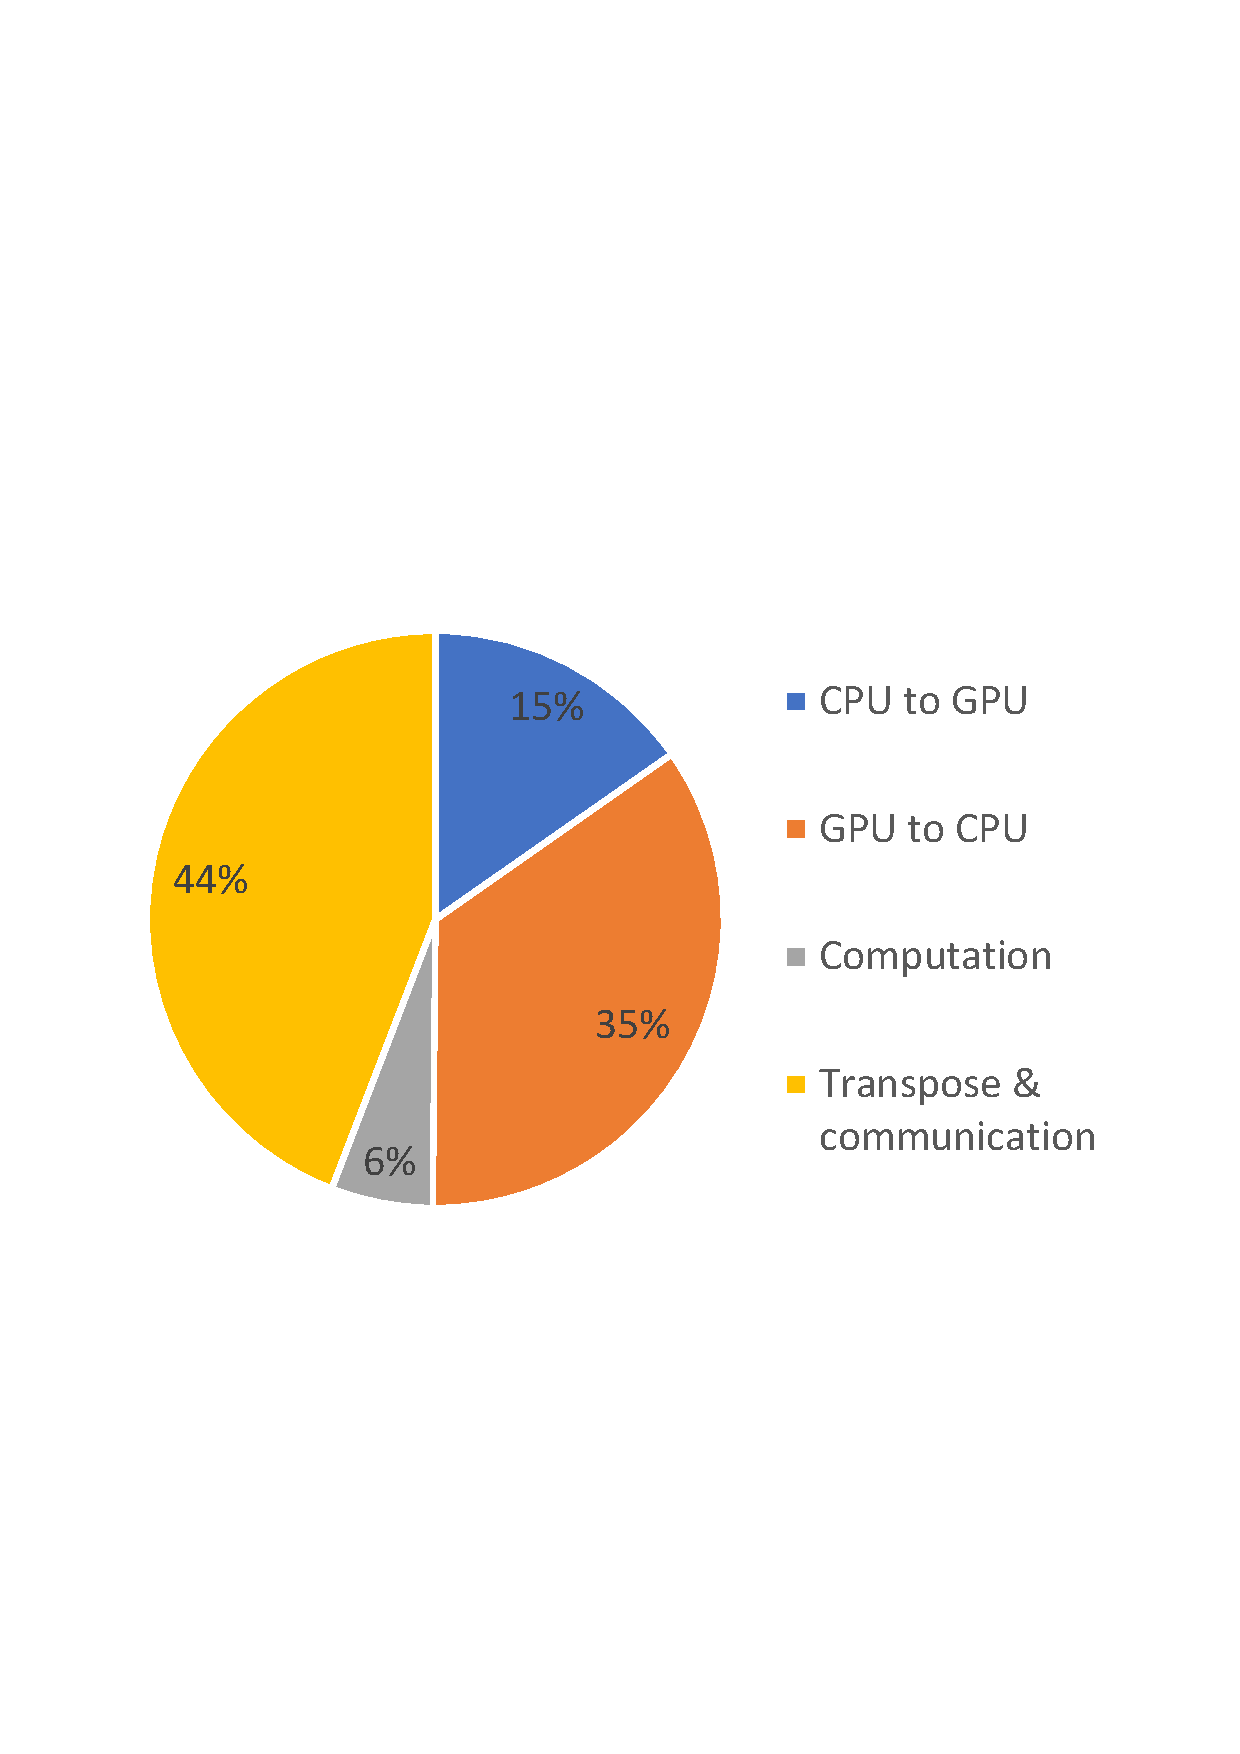
\includegraphics[width=0.55\textwidth]{Img/domain_decomposition_1GPU.pdf}
    \caption{单GPU域分解模式解泊松方程各部分耗时占比}\label{fig:1GPU_Poisson}
\end{figure}

可以看出,FFT计算所花的时间为0.487秒,相比于额外增加的数据拷贝时间1.306 + 4.627 = 4.933秒,其占比非常小,仅仅占总时间的6\%。

多GPU的一种方式是使用同一节点内使用多个GPU,因为节点内的总线宽度限制,数据拷贝时间并不会随着使用GPU数目的增加而明显减少。而复制模式只需要花费FFT计算的时间,因为FFT计算花费的时间0.487秒远小于数据拷贝的时间4.933秒,所以即使在理想情况下使用N个GPU时FFT计算的时间减少到原来的1/N,域分解模式的总时间依然是比复制模式要大。

多GPU的另一种使用跨节点的多个GPU,即每个节点有1个GPU,通过使用多个节点来使用多个GPU,这也是目前超级计算机TITAN的运行模式。
总线宽度会随着节点数增加而增加,所以数据拷贝时间会下降,假设其下降为线性的,
即在N个节点上运行的话拷贝数据时间只有原来的1/N,则总时间将会是 $4.933/N+0.487/N$,
如果我们想要取得优于复制模式的速度,即 $4.933/N+0.487/N<0.487$, GPU数目必须大于11。
类似的,如果我们想要取得两倍的速度,GPU数目必须大于22。然而,这个计算忽略了CPU和CPU之间的通讯时间,
一般来说,节点间的通讯时间随着节点数目增加而增加,因此我们很难取得理想情况的加速比。

下面,我们分别对节点内多GPU和跨节点GPU进行测试。

\subsubsection{单节点多GPU测试}
在同一节点中,我们进行了格点数为$64 \times 64 \times 64$的多GPU测试,
表\ref{tab:2GPU_Poisson}是各个部分所花费的时间,以及和单GPU时的对比。
可以看出,双GPU的总时间更大了,由8.544秒增加到了9.537秒。
其中,FFT计算的时间有0.487秒减少到了0.249秒,几乎减少了一半,
证明了多GPU对于减少纯FFT计算时间是确实有效的;对于数据拷贝时间,双GPU略有减少,
大概减少了三分之一;总时间中增加的部分来源于通讯的时间,几乎增加了一倍。
\begin{table}[!htbp]
    \centering
    \footnotesize% fontsize
    \setlength{\tabcolsep}{4pt}% column separation
    \renewcommand{\arraystretch}{1.2}%row space
    \caption{单节点双GPU域分解模式解泊松方程耗时}
    \begin{tabular}{lcc}
        \hline\hline
                          & 1GPU    & 2GPU   \\
        \hline\hline
        从CPU拷贝到GPU    & 1.306   & 0.817  \\
        \hline
        从GPU拷贝到CPU    & 2.979   & 1.991  \\
        \hline
        FFT计算           & 0.487   & 0.249  \\
        \hline
        转置和通讯        & 3.772   & 6.480  \\
        \hline
        总计              & 8.544   & 9.537  \\
        \hline\hline
    \end{tabular}
    \label{tab:2GPU_Poisson}
\end{table}

\subsubsection{跨节点多GPU测试}
我们使用超级计算机Titan测试了域分解模式下的求解解泊松方程在跨节点多GPU上的效率。
使用常用的$64 \times 64 \times 64$个格点,域分解模式下解泊松方程所花费的时间随GPU个数的变化如图\ref{fig:TITAN_GPU_Poisson64}所示,图中蓝线为总时间,各个柱代表各个部分所花费的时间,图中不清楚部分可以参考表\ref{tab:TITAN_GPU_Poisson64}。

可以看出,程序总耗时随着GPU数目增加而逐渐减少,并在32个GPU的时候到达最小值,随后开始逐渐增加。其中,拷贝数据所花费的时间基本随着GPU的数目线性减少;而通讯所花费的时间先随着GPU数目增加而逐渐减少,到达极值后又开始逐渐增加,此时通讯时间占程序所花费的时间的绝大部分;FFT计算所花费的时间随着GPU数目的增加而逐渐减少,但是FFT计算占总时间的百分比很小。

\begin{figure}[!htb]
  \centering
  \begin{tabular}{|l|l|}
    \multicolumn{2}{c}{
    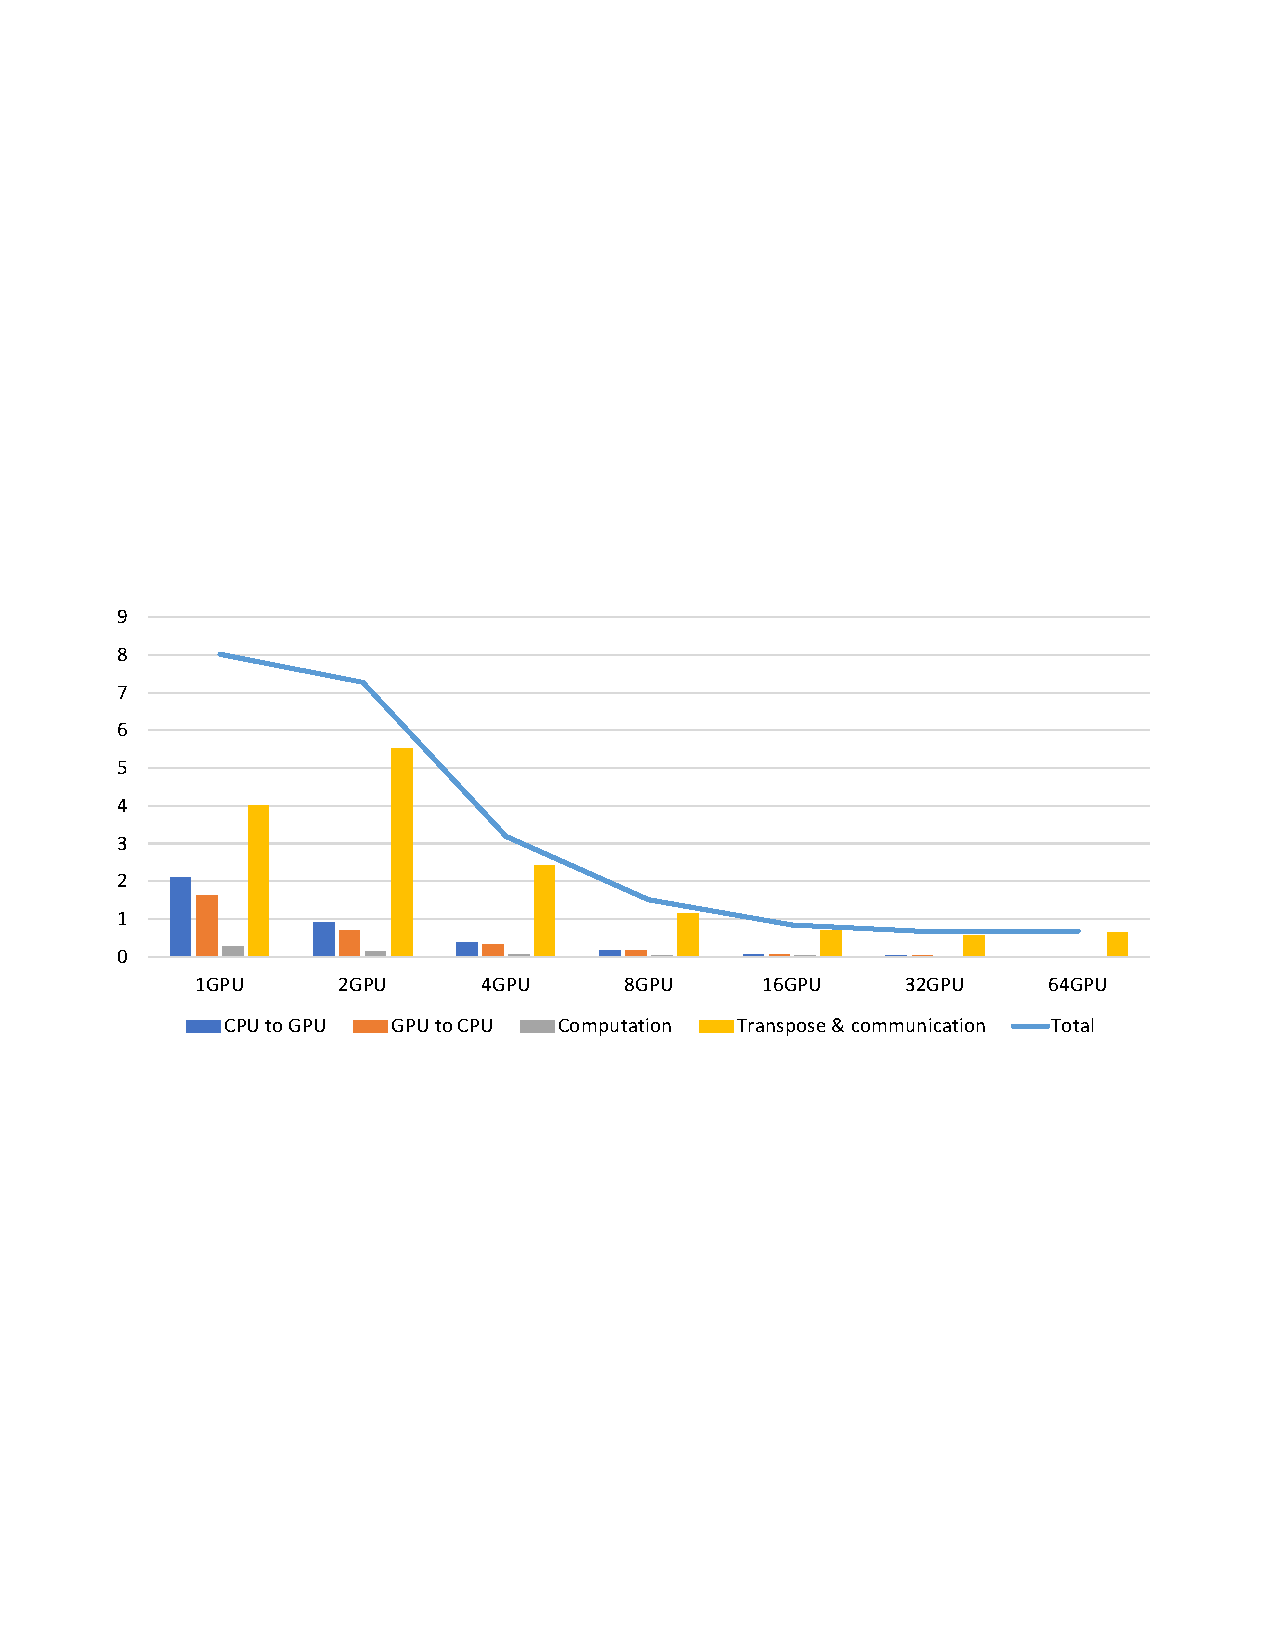
\includegraphics[width=0.9\textwidth]{Img/domain_decomposition_Titan64.pdf}} \\
  \end{tabular}
  \caption{$64 \times 64 \times 64$格点下,跨节点多~GPU~域分解模式解泊松方程时间随~GPU~个数的变化}
  \label{fig:TITAN_GPU_Poisson64}
\end{figure}

\begin{table}
  \centering
  \caption{$64 \times 64 \times 64$格点下,跨节点多GPU 域分解模式解泊松方程各部分所用时间}
  \begin{tabular}{|l|c|c|c|c|c|c|c|}
    \hline
    GPU数目	    &1	    &2	    &4	    &8 	    &16	    &32  	&64   \\
    \hline
    CPU to GPU	&2.111	&0.922	&0.390	&0.158	&0.061	&0.031	&0.0155 \\
    GPU to CPU	&1.618	&0.694	&0.314	&0.167	&0.066	&0.033	&0.0158 \\
    FFT计算  	    &0.266	&0.136	&0.069	&0.039	&0.024	&0.017	&0.0150 \\
    转置和通讯	&4.020	&5.521	&2.415	&1.146	&0.691	&0.572	&0.6320 \\
    总计	        &8.015	&7.273	&3.188	&1.51	&0.842	&0.653	&0.6783 \\
    \hline
  \end{tabular}
  \label{tab:TITAN_GPU_Poisson64}
\end{table}

我们也测试了格点数目更大的情况,格点数目越多,所需要的计算量越大。当格点数为$128 \times 128 \times 128$时,程序在不同的GPU数目下消耗的时间如图\ref{fig:TITAN_GPU_Poisson128}和表\ref{tab:TITAN_GPU_Poisson128}所示,其整体的趋势和$64 \times 64 \times 64$时类似,因为更大的计算量,其总时间在使用128个GPU时到达最小值。

\begin{figure}[!htb]
  \centering
  \begin{tabular}{|l|l|}
    \multicolumn{2}{c}{
    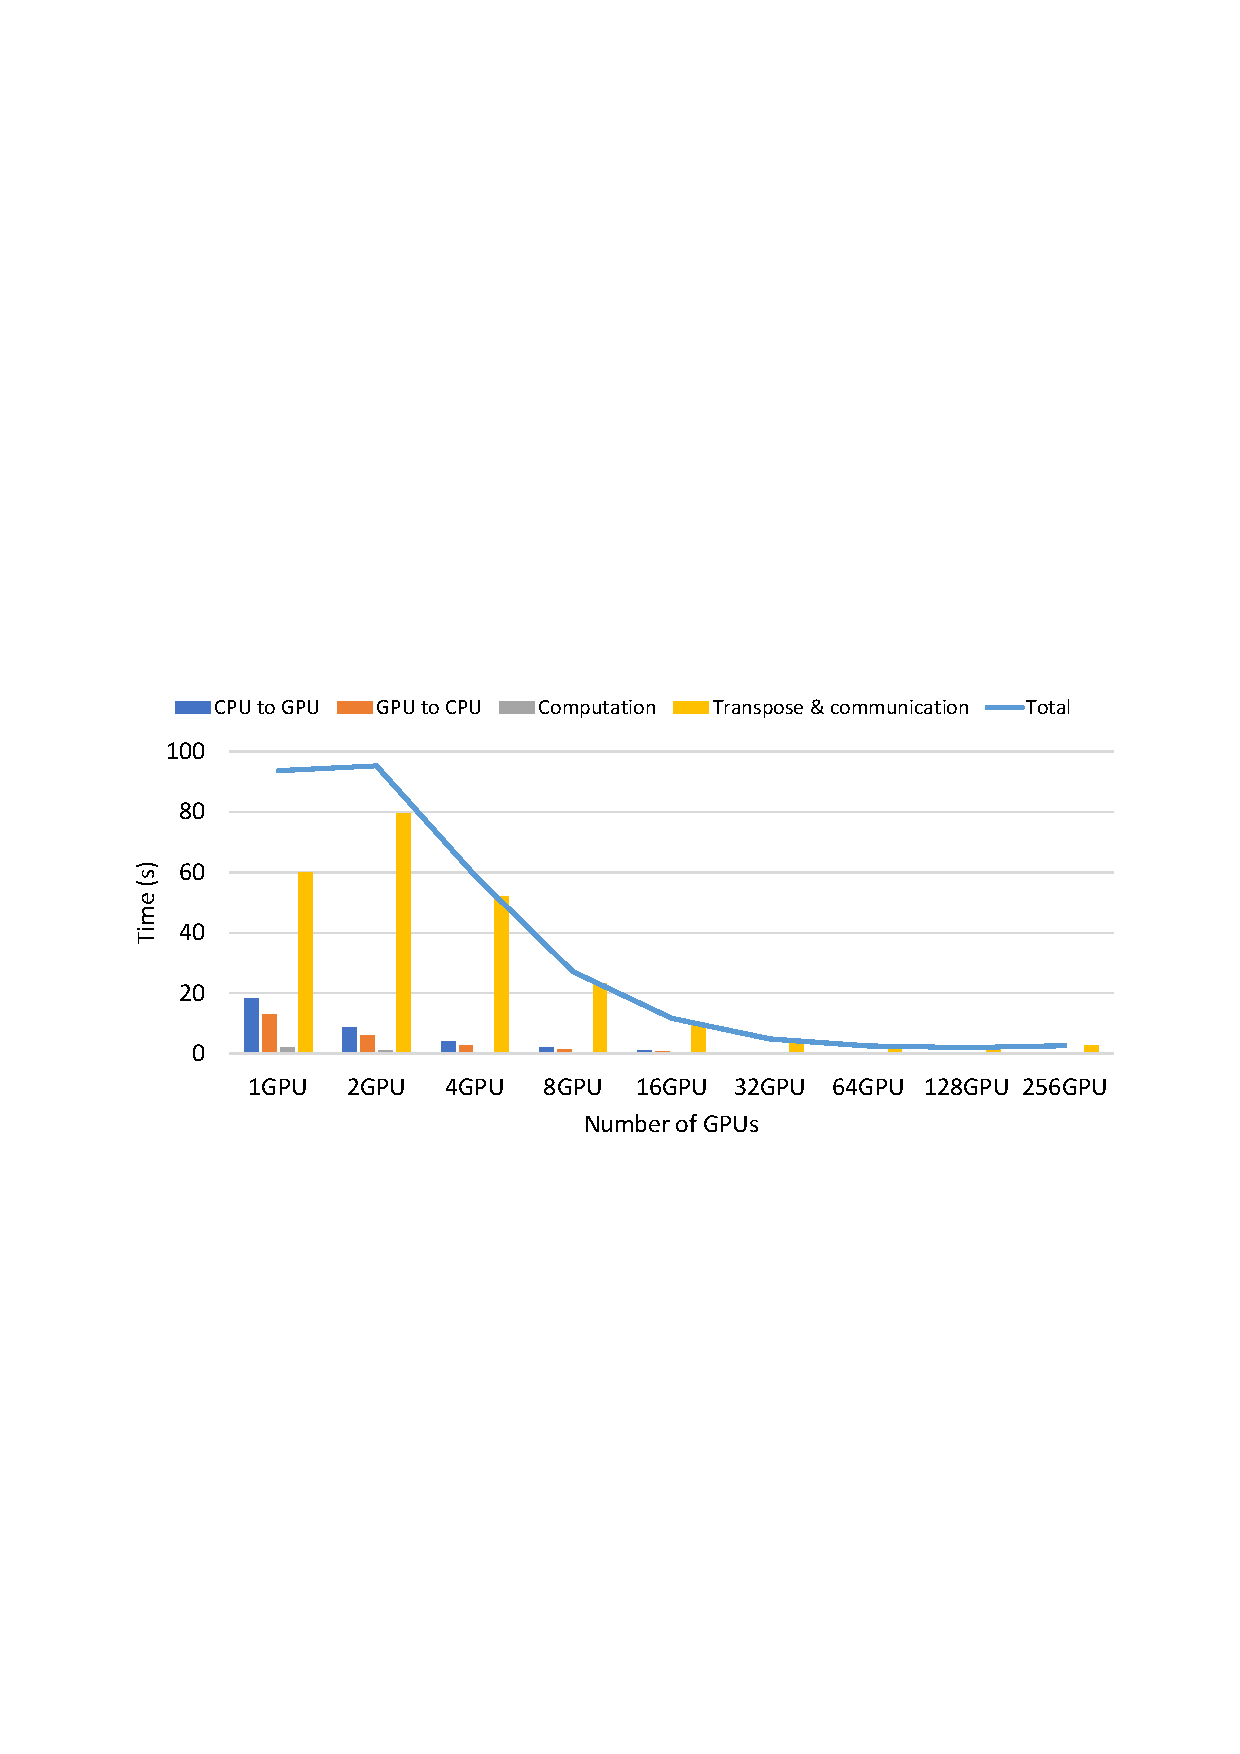
\includegraphics[width=0.9\textwidth]{Img/domain_decomposition_Titan128.pdf}} \\
  \end{tabular}
  \caption{$128 \times 128 \times 128$格点下,跨节点多~GPU~域分解模式解泊松方程时间随~GPU~个数的变化}
  \label{fig:TITAN_GPU_Poisson128}
\end{figure}

\begin{table}
  \centering
  \caption{$128 \times 128 \times 128$格点下,跨节点多GPU域分解模式解泊松方程各部分所用时间}
  \begin{tabular}{|>{\small}l|c|c|c|c|c|c|c|c|c|}
    \hline
    GPU数目	    &1	    &2	    &4	    &8 	    &16	    &32  	&64     &128	&256   \\
    \hline
    CPU to GPU	&18.29	&8.687	&3.946	&2.023	&0.953	&0.404	&0.148	&0.064	&0.033 \\
    GPU to CPU	&13.11	&6.15	&2.618	&1.463	&0.795	&0.368	&0.139	&0.07	&0.036 \\
    FFT计算  	    &2.185	&1.034	&0.522	&0.266	&0.138	&0.071	&0.036	&0.021	&0.017 \\
    转置和通讯	&59.99	&79.34	&51.85	&23.30	&9.797	&4.041	&2.237	&1.859	&2.506 \\
    总计	        &93.58	&95.21	&58.94	&27.05	&11.68	&4.884	&2.56	&2.014	&2.592\\
    \hline
  \end{tabular}
  \label{tab:TITAN_GPU_Poisson128}
\end{table}

在$64 \times 64 \times 64$和$128 \times 128 \times 128$两种情况下,总时间开始都随着GPU数目增加而减小,然后到达最小值,随后由于通讯所需要的时间变大,总时间也随之变大。
然而,无论是使用$64 \times 64 \times 64$个格点还是$128 \times 128 \times 128$个格点,总时间的最小值都大于只是用一个GPU的纯计算时间。
\subsubsection{小结}
通过上面对于“域分解模式”的实现和测试,可以看出程序运行速度主要受限于CPU和GPU之间数据拷贝的速度与CPU和CPU之间的通讯速度。
如果GPU带宽足够大,或者以后能够实现GPU与GPU之间的直接通讯的话,“域分解模式”可以作为一个可行的方案。
但是在目前,与“复制模式”相比,“域分解模式”由于其额外的数据拷贝和通讯开销,并不能通过减少运算量来达到提高速度的目的。
所以我们在程序中以及在下文中都使用“复制模式”(除非另加说明),即使所有的GPU都同时运行同样的程序。

\subsection{单GPU性能-GTX1060}      \label{section:PIC_Performance_GTX1060}
在测试了泊松方程求解器之后,我们通过对比CPU程序和单个GPU程序的运行速度,来得到GPU程序的加速比。
测试使用的格点数为~ $64 \times 64 \times 64$,加速比等于CPU程序耗时除以GPU程序耗时。
图\ref{fig:PIC_speedup_1GPU}和表\ref{tab:PIC_speedup_1GPU}是粒子数从16k到1.6m时CPU程序和GPU程序各部分耗时以及加速比。
可以看出,程序总耗时的加速比大约有40,程序各个部分的加速比有很大不同。

其中,橙色柱行代表求解泊松方程,其加速比大约是64,而且并不随粒子数目的变化而变化。
事实上,求解泊松方程的计算量主要和格点数相关,而此次测试中我们都是用同样的格点数,
因此其耗时和加速比基本不变,之后我们会比较在不同格点数情况下求解泊松方程的加速比变化。
灰色柱行代表推动粒子的加速比,其随着粒子数目增加而变大,在粒子数较大时取得超过了70的加速比。
浅蓝色和深蓝色柱行分别是权重插值和粒子信息输出的加速比,其中GPU的权重插值部分包括了粒子排序运算,
而且由于其运算的不规则性,加速比较低;而粒子信息输出部分也包含了束团参数的计算,这部分加速比较低是因为输出带宽的限制。


\begin{figure}[!htb]
  \centering
  \begin{tabular}{|l|l|}
    \multicolumn{2}{c}{
    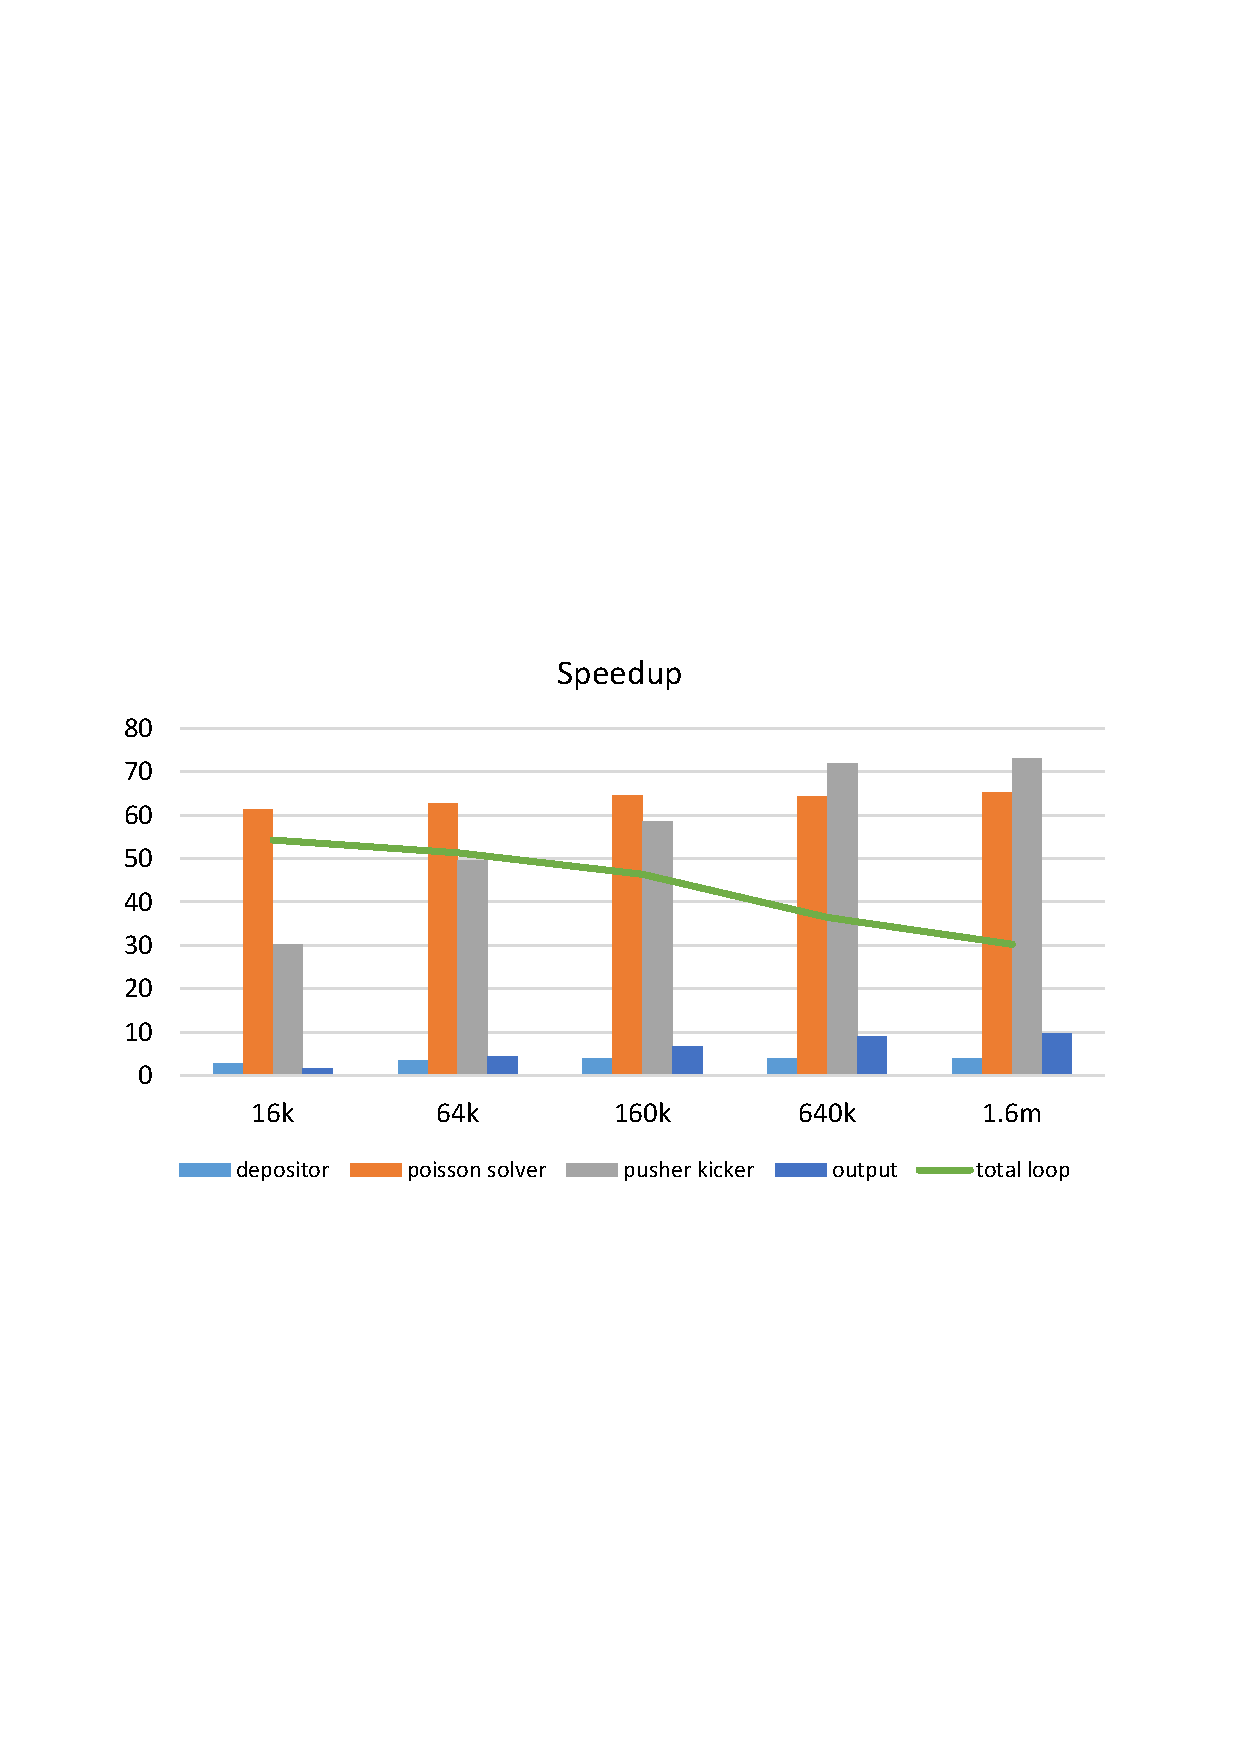
\includegraphics[width=0.9\textwidth]{Img/PIC_speedup_1GPU.pdf}} \\
  \end{tabular}
  \caption{PIC程序在单GPU上的加速比}
  \label{fig:PIC_speedup_1GPU}
\end{figure}

\begin{table}
  \centering
  \caption{PIC程序在单GPU上的加速比}
  \begin{tabular}{|l|r|r|r|}
    \hline
    16k                      &    CPU(s)      &     GPU(s)    &  Speedup    \\
    \hline
    depositor (include sort) &    0.16888     &     0.05874   &  2.875043   \\
    Poisson solver           &    26.13173    &     0.42511   &  61.47051   \\
    pusher kicker            &    0.53748	  &     0.01781	  &  30.17855   \\
    output                   &    0.01977     &     0.01149   &  1.720627   \\
    total loop               &    27.78216    &     0.51199   &  54.26309   \\
    \hline
    64k                      &    CPU(s)      &     GPU(s)    &  Speedup    \\
    \hline
    depositor (include sort) &    0.3897      &     0.10847   &  3.592698   \\
    Poisson solver           &    26.08269    &     0.41554   &  62.76818   \\
    pusher kicker            &    2.00422	  &     0.04032	  &  49.70784   \\
    output                   &    0.0641      &     0.01433   &  4.473133   \\
    total loop               &    29.54123    &     0.57598   &  51.28864   \\
    \hline
    160k                     &    CPU(s)      &     GPU(s)    &  Speedup    \\
    \hline
    depositor (include sort) &    0.82705     &     0.20731   &  3.989436   \\
    Poisson solver           &    25.9208     &     0.40208   &  64.46677   \\
    pusher kicker            &    4.88644	  &     0.08343	  &  58.56934   \\
    output                   &    0.15477     &     0.02316   &  6.682642   \\
    total loop               &    32.94187    &     0.71      &  46.397     \\
    \hline
    640k                     &    CPU(s)      &     GPU(s)    &  Speedup    \\
    \hline
    depositor (include sort) &    2.79413     &     0.71529   &  3.90629    \\
    Poisson solver           &    25.72129    &     0.40045   &  64.23097   \\
    pusher kicker            &    22.48269	  &     0.31207	  &  72.04374   \\
    output                   &    0.62289     &     0.06931   &  8.987015   \\
    total loop               &    53.51193    &     1.46745   &  36.46593   \\
    \hline
    1.6M                     &    CPU(s)      &     GPU(s)    &  Speedup    \\
    \hline
    depositor (include sort) &    6.7528      &     1.73779   &  3.885855   \\
    Poisson solver           &    26.03071    &     0.39894   &  65.24969   \\
    pusher kicker            &    56.05512	  &     0.76562	  &  73.21533   \\
    output                   &    1.56528     &     0.16288   &  9.61002    \\
    total loop               &    90.40391    &     2.99053   &  30.23006   \\
    \hline
  \end{tabular}
  \label{tab:PIC_speedup_1GPU}
\end{table}

权重插值和粒子信息输出的加速比较低,从而拉低了整体的加速比。整体的加速比随着粒子数的增加而逐渐变小,其原因是当粒子数目较小时的时候,求解泊松方程所占得比重较大,从而整体加速比较大;而当粒子数目变大的时候,权重插值所占的时间比重变大,因而整体加速比随之变小。程序各部分耗时在不同粒子数所占比重如图\ref{fig:PIC_speedup_1GPU_percentage}所示。

\begin{figure}[!htb]
    \centering
    \begin{subfigure}[b]{0.75\textwidth}
        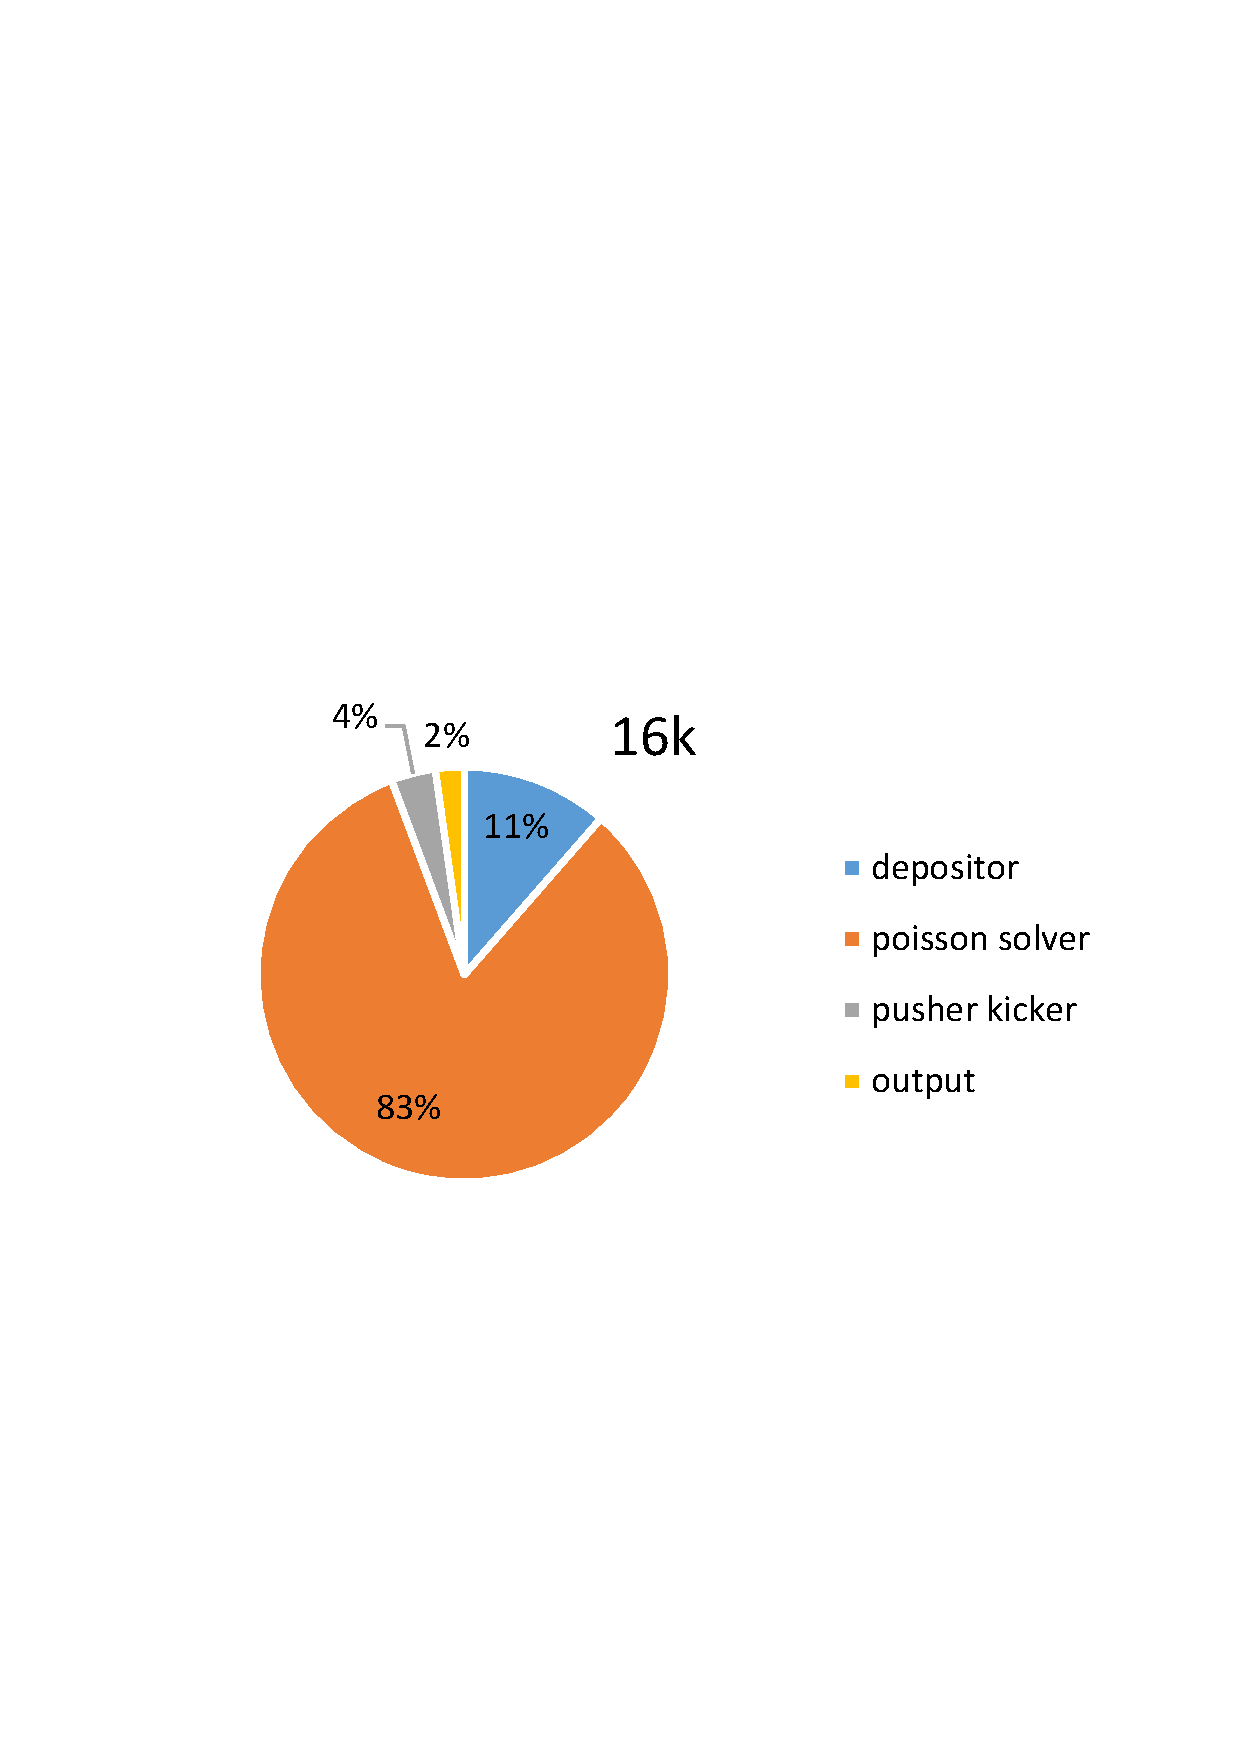
\includegraphics[width=\textwidth]{Img/PIC_speedup_1GPU_percentage1.pdf}
        %\caption{}
    \end{subfigure}
    \quad
    \begin{subfigure}[b]{0.75\textwidth}
        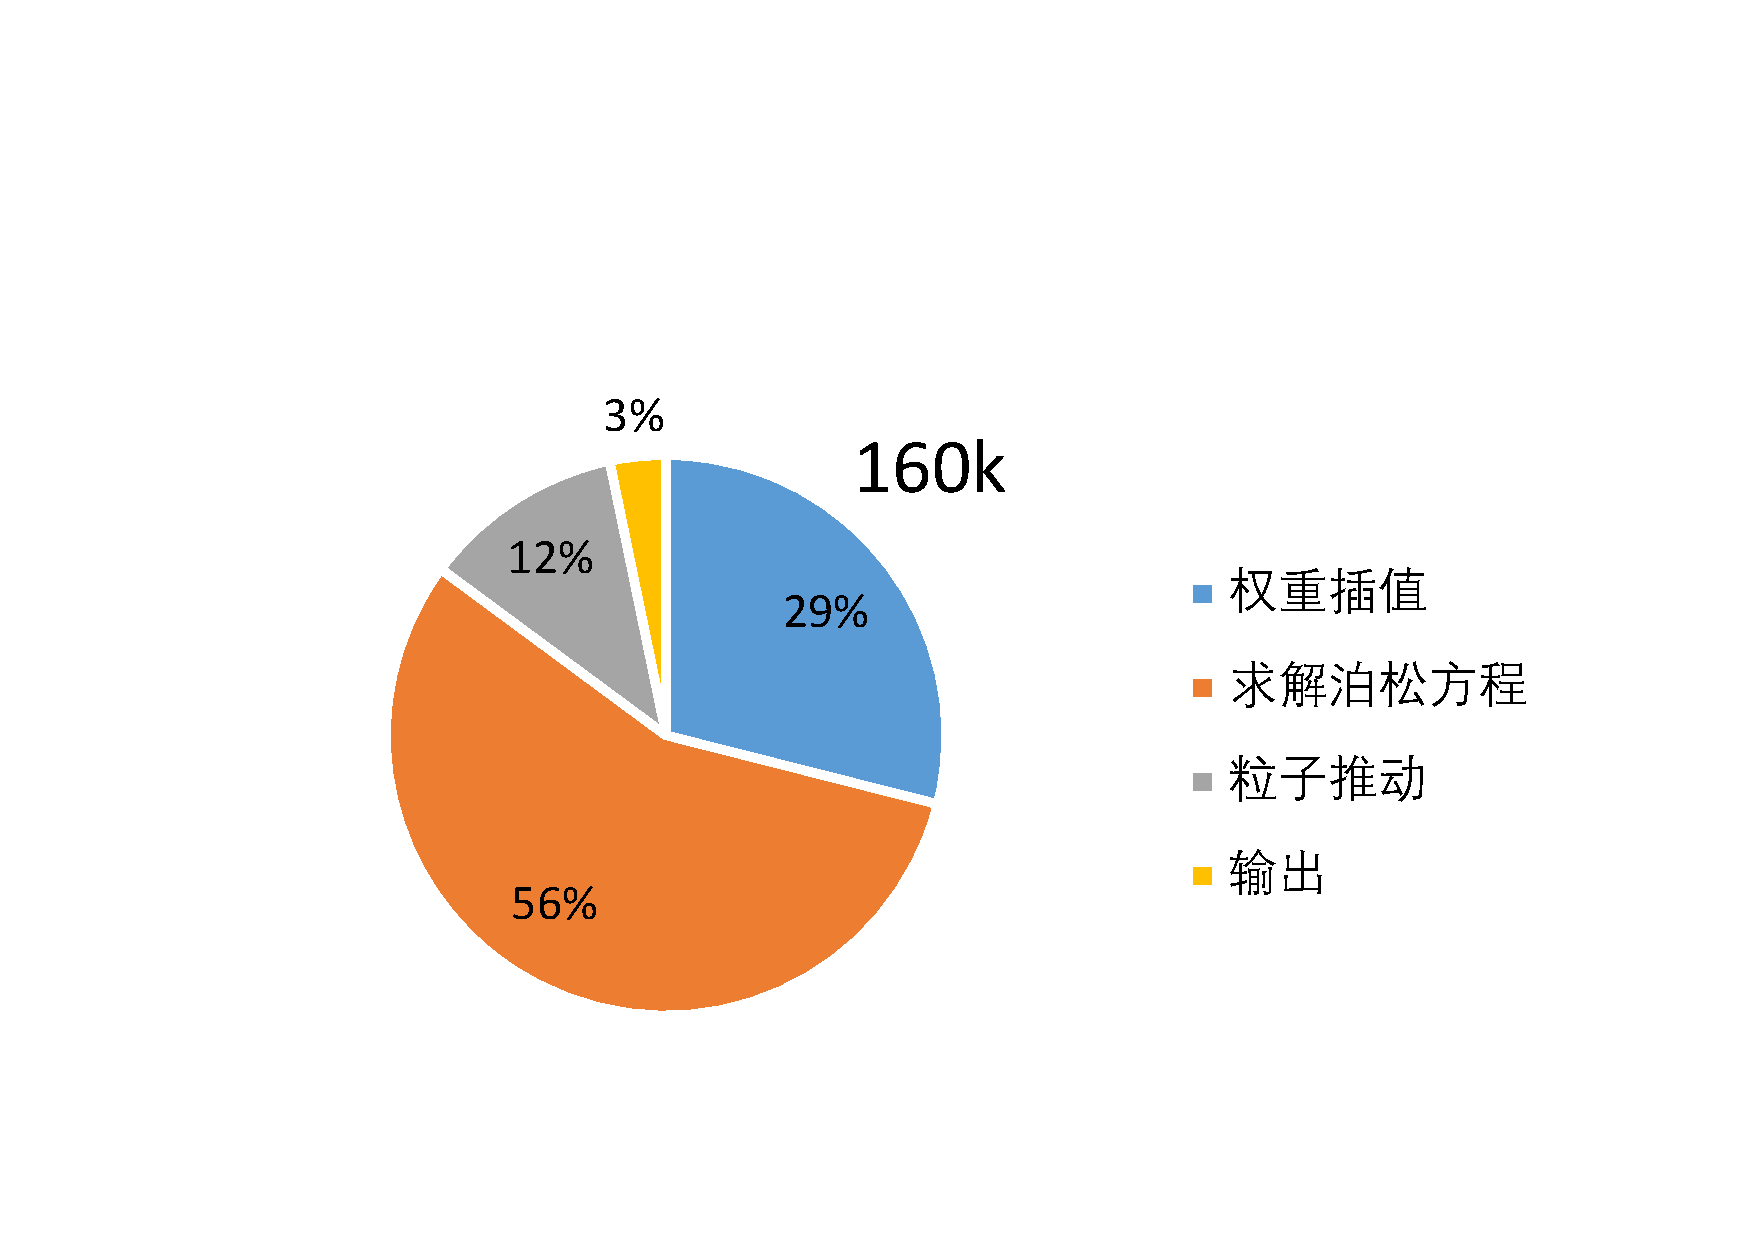
\includegraphics[width=\textwidth]{Img/PIC_speedup_1GPU_percentage2.pdf}
        %\caption{}
    \end{subfigure}
    \quad
    \begin{subfigure}[b]{0.75\textwidth}
        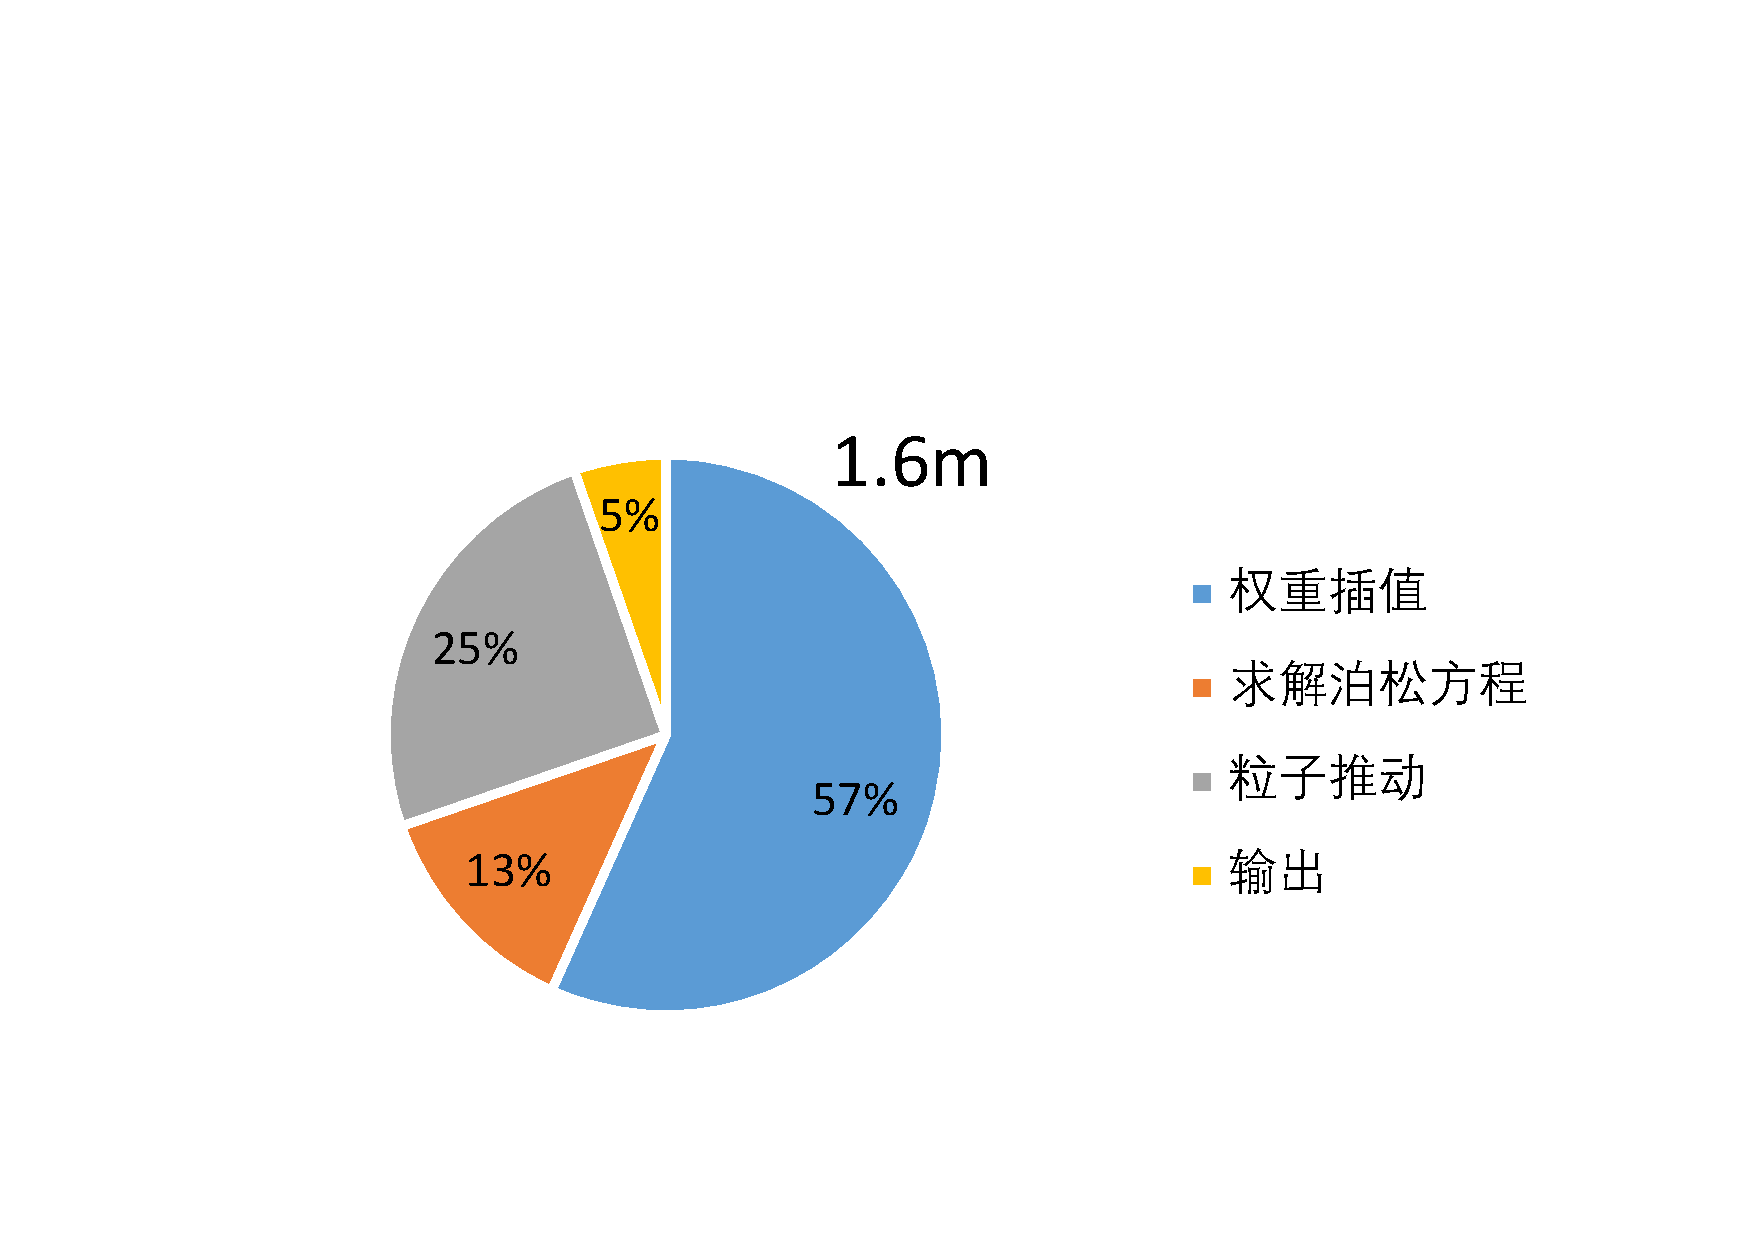
\includegraphics[width=\textwidth]{Img/PIC_speedup_1GPU_percentage3.pdf}
        %\caption{}
    \end{subfigure}
    \caption{程序各部分耗时在不同粒子数时所占百分比}\label{fig:PIC_speedup_1GPU_percentage}
\end{figure}

在上述测试中使用的都是$64 \times 64 \times 64$个格点数,因此求解泊松方程的时间和加速比都基本不变。
在不同的格点数情况下,求解泊松方程的加速比如图\ref{fig:PIC_speedup_1GPU_Poisson}所示。
可以看出,求解泊松方程的加速比随着格点数的增加逐渐变大,最终达到了接近70,这是因为格点数越大,其计算量越多,GPU上的负载能够分布得更均匀。
对于实际模拟中常用的$64 \times 64 \times 64$个格点和$128 \times 128 \times 128$个格点中,我们都取得了令人满意的加速比。

\begin{figure}[!htb]
  \centering
  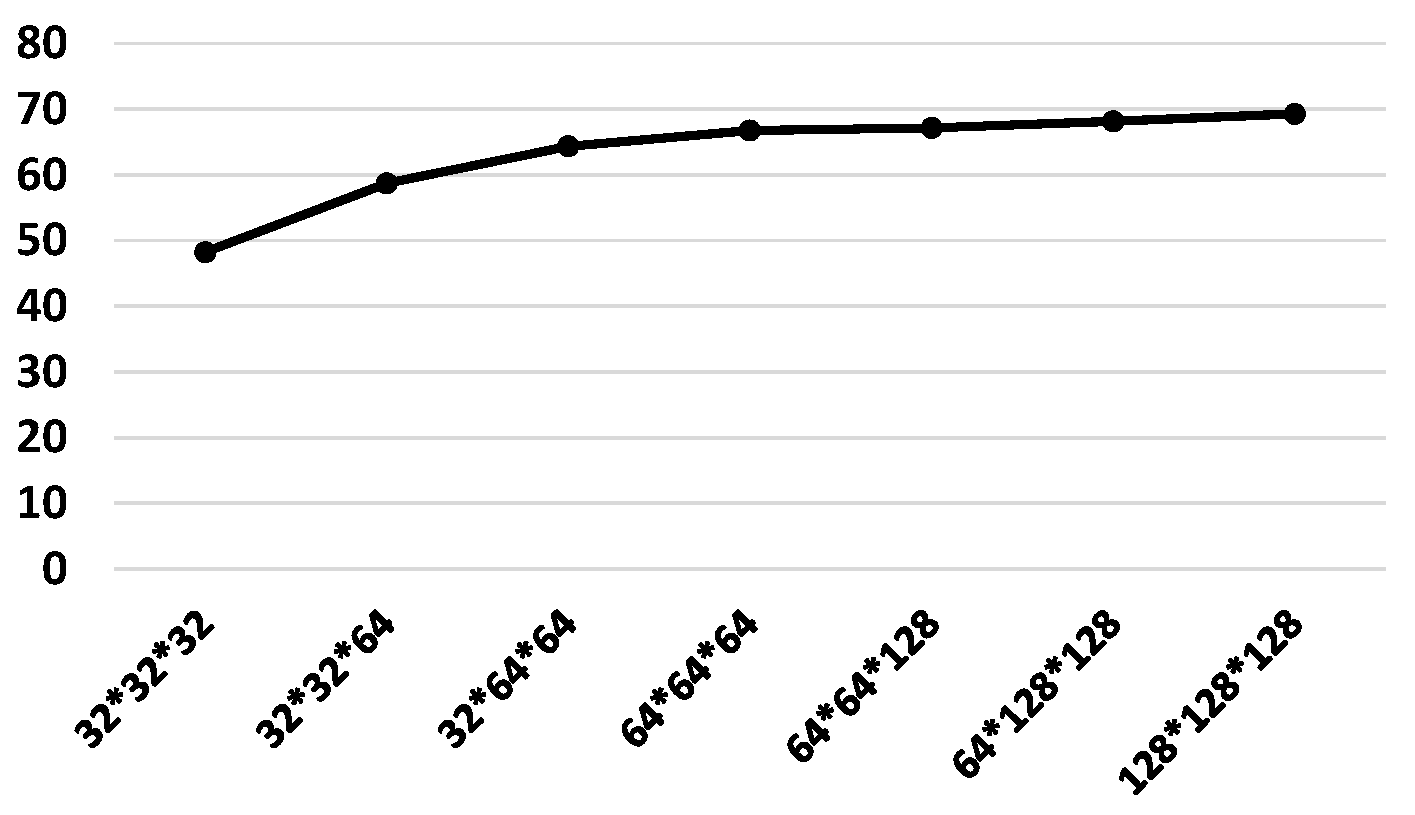
\includegraphics[width=0.9\textwidth]{Img/PIC_speedup_1GPU_Poisson.pdf}
  \caption{不同的格点数情况下单GPU求解泊松方程的加速比}
  \label{fig:PIC_speedup_1GPU_Poisson}
\end{figure}

总之,在单GPU上,程序总体的加速比达到了40,而求解泊松方程的加速比超过了60。在一个普通的家用机GPU上运行的速度相当于在64核机器上的两倍。
另外,如小节\ref{section:PIC_GPU_reorder}所述,因为GPU内存大小一般是固定的,
而不像CPU内存那样较容易的扩展,所以单GPU的粒子数目存在某个上限,当超过最大粒子数时,
应该使用多GPU来进行计算。在接下来的一节中,我们将讨论PIC程序在多GPU上的效率。

\subsection{GPU集群性能-Titan}
在单GPU测试之后,我们使用GPU集群Titan对PIC Cuda程序进行了多GPU性能测试。
Titan使用CPU和GPU混合架构,是目前世界上速度最快、规模最大的计算机集群之一。
Titan中每个节点只有一个GPU,因此只能通过使用多个节点来使用多个GPU。
在这种条件下,GPU之间的通讯只能够通过先将数据拷贝到CPU端,再通过CPU端的节点间网络进行通讯。

图\ref{fig:PIC_speedup_Titan_160k_1}为求解泊松方程时各个部分所花费的时间随GPU个数的变化。
可以看出,因为处于复制模式,求解泊松方程的耗时基本保持不变;
更多的GPU个数意味着每个GPU上的粒子数随之减小,所以粒子推动的耗时随着GPU数目的增加而减少;
而由于通讯成本随着GPU数目增加而增加,信息统计和输出耗时也随之增加。
各个部分对于GPU的数目变化的反应并不相同,单从总体来看,程序总耗时基本保持不变。

\begin{figure}[!htb]
  \centering
  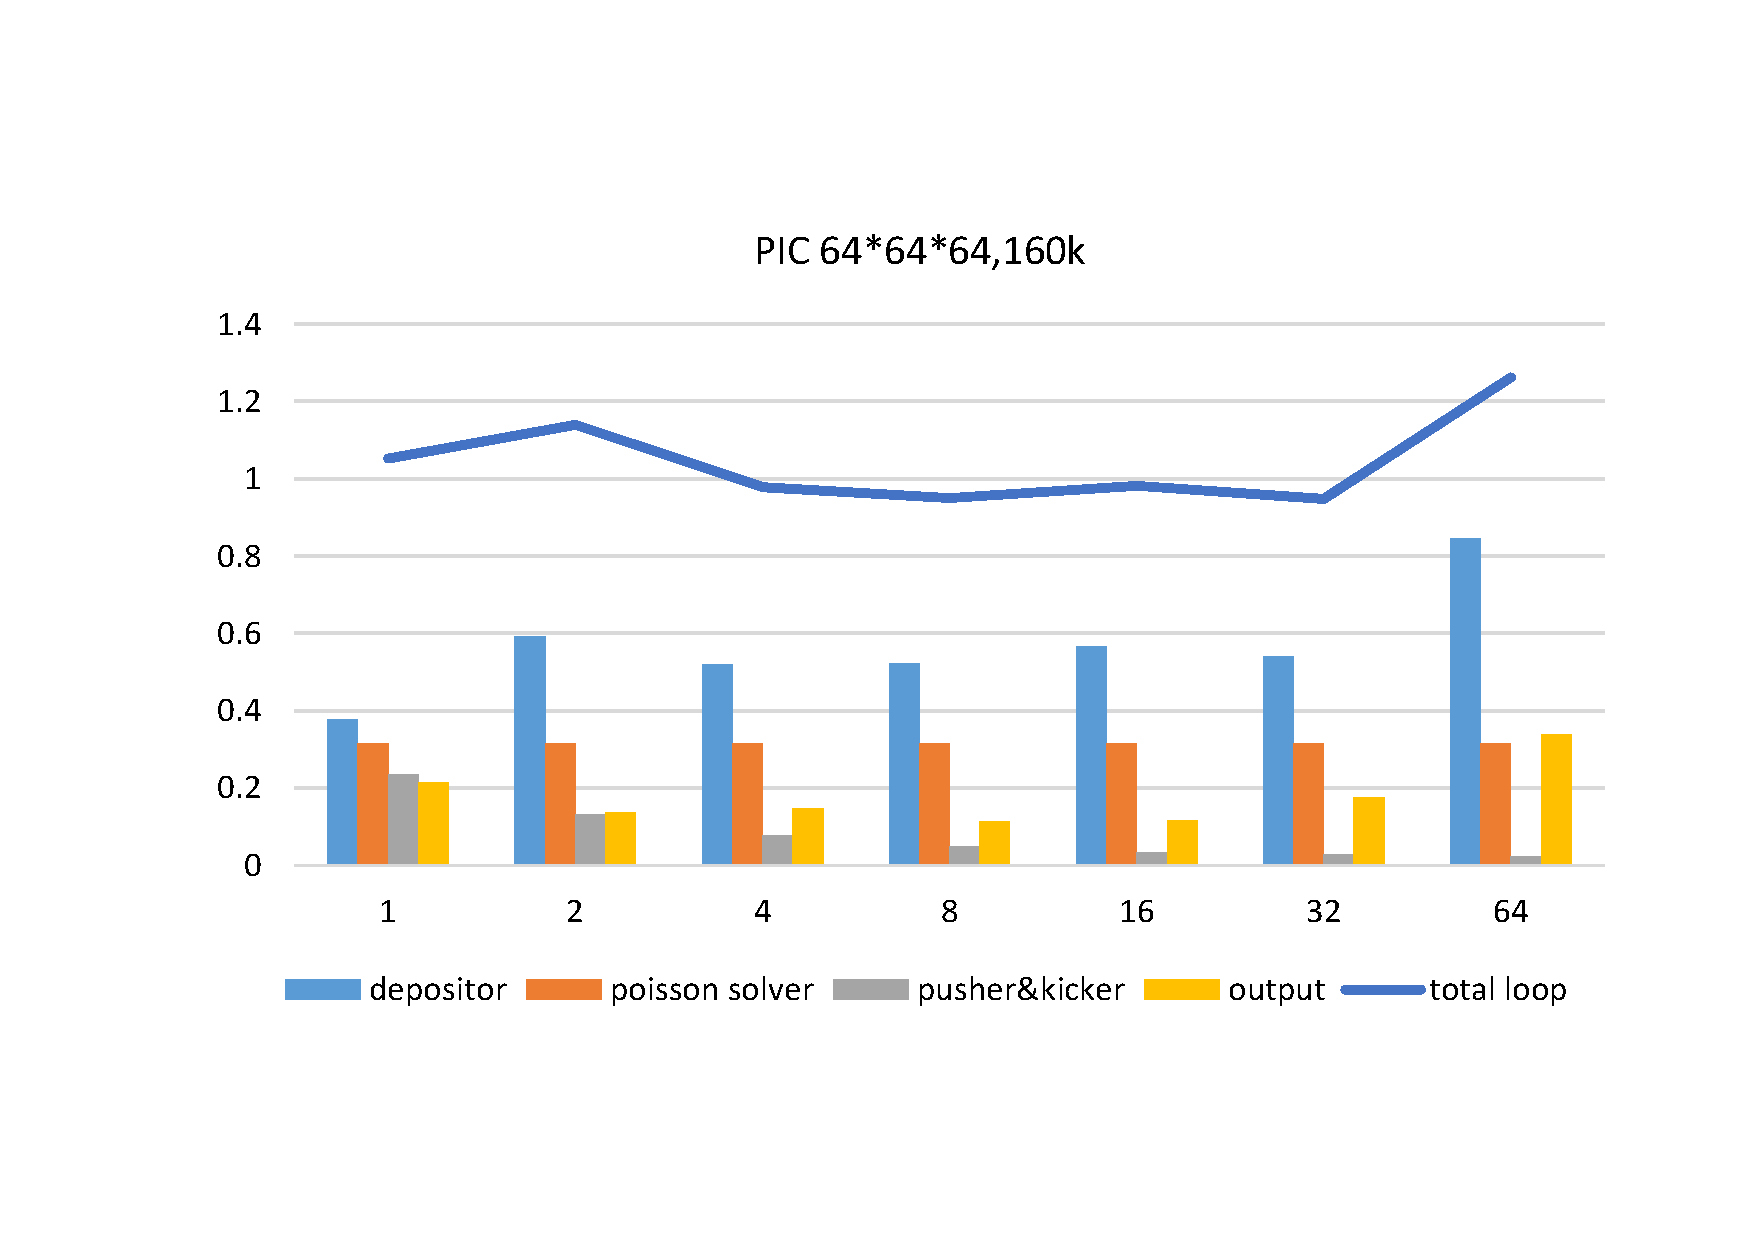
\includegraphics[width=0.9\textwidth]{Img/PIC_speedup_Titan_160k_1.pdf}
  \caption{$64 \times 64 \times 64$个格点,160K个粒子时,Titan上PIC程序耗时随GPU个数的变化}
  \label{fig:PIC_speedup_Titan_160k_1}
\end{figure}

图\ref{fig:PIC_speedup_Titan_160k_2}和图\ref{fig:PIC_speedup_Titan_160k_1}类似,也是$64 \times 64 \times 64$各个点,160k个粒子下程序总耗时随着~GPU~数目的变化。
但是在图\ref{fig:PIC_speedup_Titan_160k_2}中,GPU数目大于等于2的时候,求解泊松方程使用了域分解模式。其在各种情况下,都相较复制模式耗时更多,主要是拷贝数据花费了大量时间,这个结果和我们在小节\ref{section:PIC_GPU_Poisson}中讨论的相符。

\begin{figure}[!htb]
  \centering
  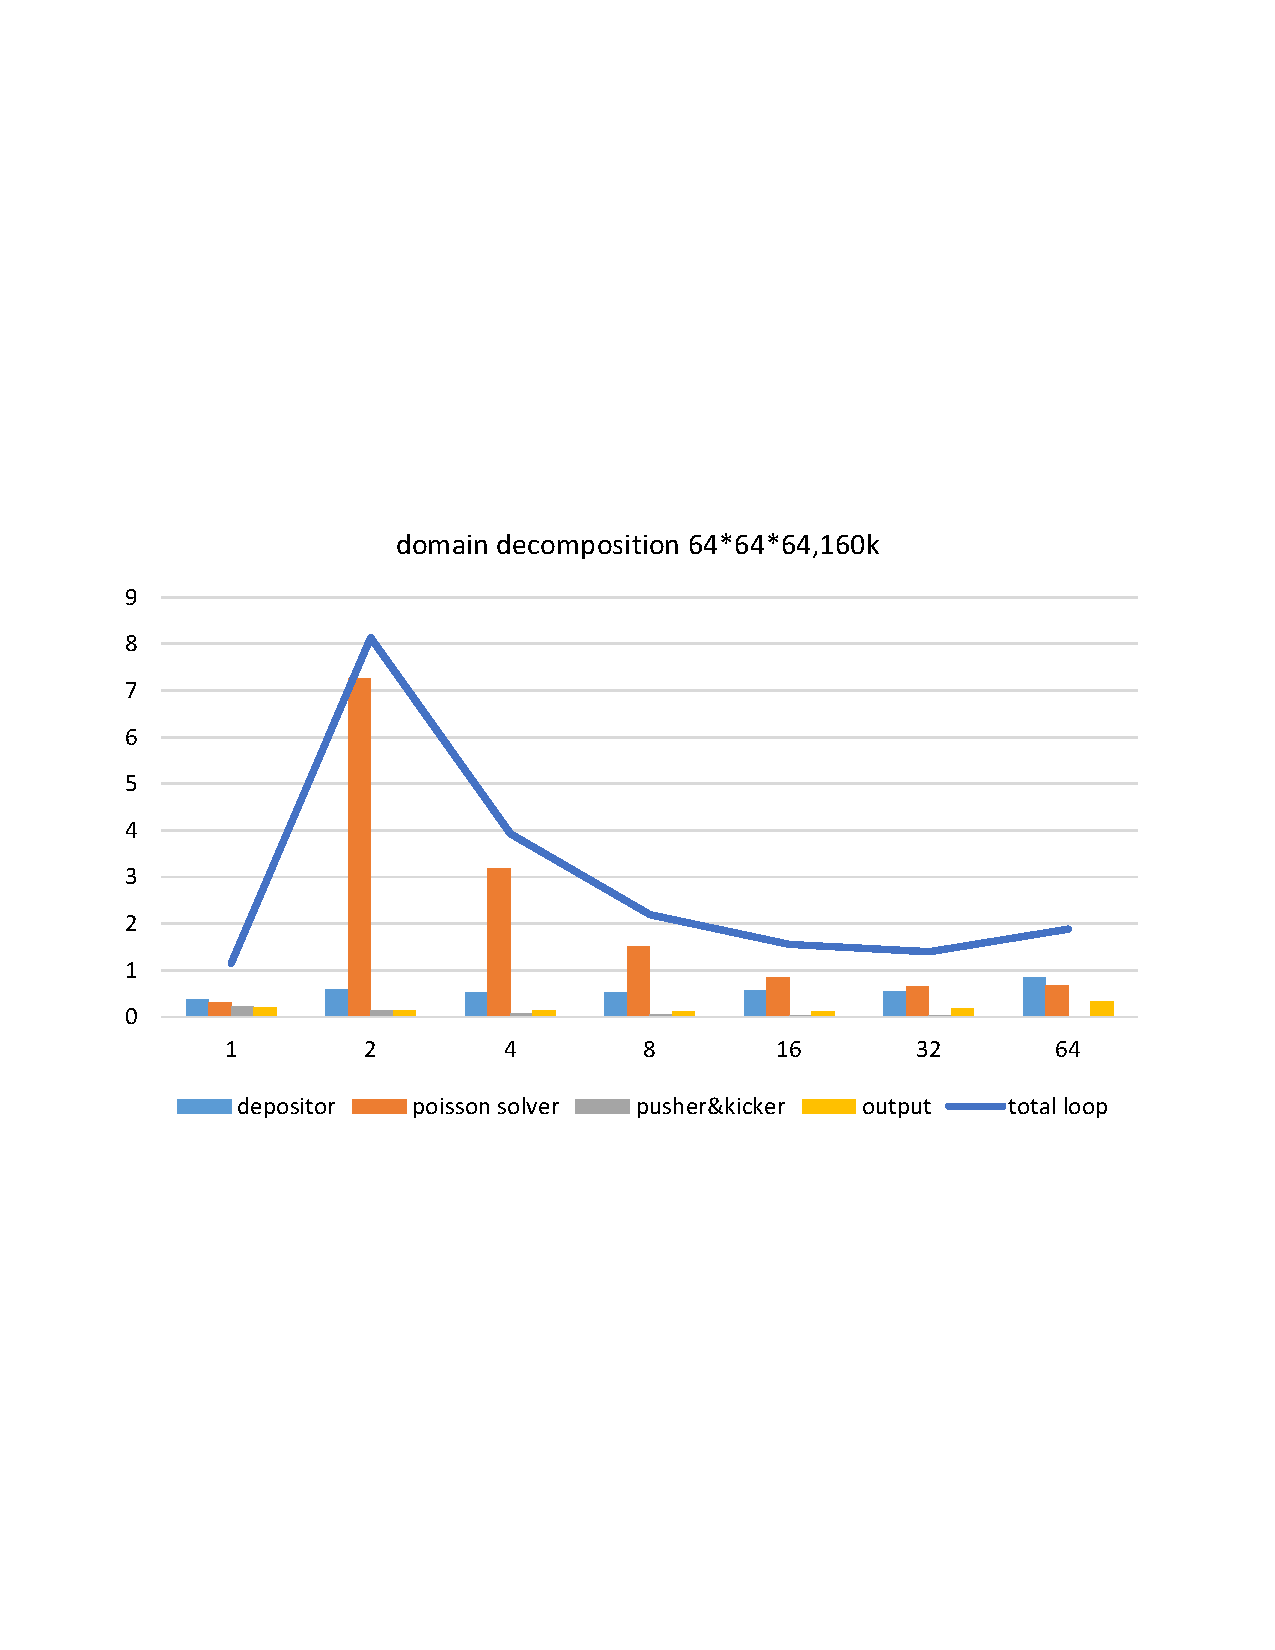
\includegraphics[width=0.9\textwidth]{Img/PIC_speedup_Titan_160k_2.pdf}
  \caption{$64 \times 64 \times 64$个格点,160K个粒子时,Titan上域分解模式PIC程序耗时随GPU个数的变化}
  \label{fig:PIC_speedup_Titan_160k_2}
\end{figure}

当粒子数更大时,耗时的趋势发生了变化。图\ref{fig:PIC_speedup_Titan_1_6m}是粒子数为一百六十万(~1.6m)的结果,
粒子数较图\ref{fig:PIC_speedup_Titan_160k_1}变大了十倍。在使用1.6m个粒子时,
总耗时随着使用的~GPU数目增加而明显下降,并在32个GPU处到达最小值。
这是因为在大粒子数目情况下,推动粒子和权重插值所消耗的时间占总时间的比重更大。
而由于使用多GPU带来的每个GPU上的粒子数目变少,推动粒子和权重插值能够很好的被多GPU加速。

\begin{figure}[!htb]
  \centering
  \includegraphics[width=0.9\textwidth]{Img/PIC_speedup_Titan_1_6m.pdf}
  \caption{$64 \times 64 \times 64$个格点,1.6M个粒子时,Titan上PIC程序耗时随GPU个数的变化}
  \label{fig:PIC_speedup_Titan_1_6m}
\end{figure}

我们尝试了使用更大的粒子数,一千六百万个粒子(16m),更十倍于前,如图\ref{fig:PIC_speedup_Titan_16m}所示。
由于GPU内存大小的限制,程序在这个粒子数下不能仅仅使用1或2个~GPU运行,因此在图\ref{fig:PIC_speedup_Titan_16m}中,
GPU数目等于1和等于2的时候没有数据。对于更多的GPU数目,程序耗时随着GPU数目增加而减小。

超级计算机Titan上使用的GPU型号为NVIDIA K20x,每个GPU有5GB的内存。
理想情况下,一个5GB内存能够使用的最大粒子数为六千万(60m)。
但这个粒子数是在使用空间均匀分布下才能达到,而实际上,我们很难达到这个粒子数。
在一个实际的加速器模拟中,我们通常使用WaterBag 或者高斯分布,因此其可用的粒子数目远小于理想数目。

\begin{figure}[!htb]
  \centering
  \includegraphics[width=0.9\textwidth]{Img/PIC_speedup_Titan_16m.pdf}
  \caption{$64 \times 64 \times 64$个格点,16M个粒子时,Titan上PIC程序耗时随GPU个数的变化}
  \label{fig:PIC_speedup_Titan_16m}
\end{figure}

\subsection{GPU集群性能-SummitDev}
和上一节中在Titan上进行的性能研究类似,我们还在ORNL新一代的GPU集群SummitDev上对PIC-Cuda程序进行了测试。
图~\ref{fig:PIC_SummitDev_160K}为使用 $64\times64\times64$ 个格点和  160K 个粒子的程序耗时。
和Titan的耗时趋势一样,随着GPU数量的增加,粒子推动所消耗的时间减少,权重粒子所消耗的时间有所增加。
而总时间并不随着GPU数量的增加而减少。多GPU不能提高效率的原因是SummitDev上GPU的计算能力非常强大,
对于160K个粒子来说,纯计算在整体耗时中所占比例不大,使用一个GPU已经足够。

\begin{figure}[!htb]
  \centering
  \includegraphics[width=0.9\linewidth]{Img/PIC_SummitDev_160K.pdf}
  \caption{$64 \times 64 \times 64$个格点,160K个粒子时,SummitDev上PIC程序耗时随GPU~个数的变化}
  \label{fig:PIC_SummitDev_160K}
\end{figure}

当粒子数量变大时,耗时趋势发生了变化。
图~\ref{fig:PIC_SummitDev_1600K}显示了160万个粒子的结果。总耗时随着GPU数量的增加而减少,并在16个GPU时到达最小值。
与Titan上的运行时间相比,由于计算能力的提高,对于同一规模的问题在SummitDev上所需要的时间减少了50\% 。
图~\ref{fig:PIC_SummitDev_16M}为了1600万个粒子的结果,受GPU内存大小的限制,程序必须使用两个或两个以上GPU运行。
在粒子数很大的情况下,由于计算量较大,程序能够充分使用多个GPU的性能,所以总耗时随着GPU数目的增加而单调递减。

\begin{figure}[!htb]
  \centering
  \includegraphics[width=0.9\linewidth]{Img/PIC_SummitDev_1600K.pdf}
  \caption{$64 \times 64 \times 64$个格点,1.6M个粒子时,SummitDev上PIC程序耗时随GPU~个数的变化}
  \label{fig:PIC_SummitDev_1600K}
\end{figure}

\begin{figure}[!htb]
  \centering
  \includegraphics[width=0.9\linewidth]{Img/PIC_SummitDev_16M.pdf}
  \caption{$64 \times 64 \times 64$个格点,16M个粒子时,SummitDev上PIC程序耗时随GPU~个数的变化}
  \label{fig:PIC_SummitDev_16M}
\end{figure}

\subsection{CPU集群性能-KNL}        \label{section:PIC_Performance_CPUcluster}
为了和GPU做比较,我们也在CPU集群KNL上使用MPI~和OpenMP混合并行实现了高效率的PIC程序。
首先,我们使用集群的一个节点来研究不同 OpenMP 线程数和MPI进程数下程序的效率和内存占用情况,并找到最优混合并行配置。
之后,我们使用多个节点,研究程序在不同节点数下的效率变化。

\subsubsection{单节点}
首先,我们使用$64 \times 64 \times 64$个网格,在1.6m粒子数下测试不同的混合并行配置,
如图\ref{fig:PIC_speedup_Cori_1node_1_6m}所示。其中横轴为不同的并行配置,
其中MPI进程数由1指数增加到64,而~OpenMP~线程数有64指数得减小到1,线程数乘以进程数则保持不变。
在每种并行配置下,总时间(浅蓝色实线),和权重插值,求解泊松方程,推动粒子,
信息输出(各色柱行)所耗时间由左纵轴以秒为单位表示,而内存占用(绿色实线)由右纵轴以GB为单位表示。

\begin{figure}[!htb]
  \centering
  \includegraphics[width=0.9\textwidth]{Img/PIC_speedup_Cori_1node_1_6m.pdf}
  \caption{1.6m粒子数下,单节点下不同混合并行配置的耗时与内存占用}
  \label{fig:PIC_speedup_Cori_1node_1_6m}
\end{figure}

从图\ref{fig:PIC_speedup_Cori_1node_1_6m}可以看出,除了纯OpenMP并行(MPI=1,OMP=64)明显较慢外,
其他各个并行配置下所消耗的总时间的差别并不大,其中耗时最小的并行配置为使用32个MPI进程,每个进程使用2个OpenMP线程。
%一般而言,使用较大的MPI进程数是比较有效率的选择。
而内存占用基本随着MPI进程数目线性增加。

程序的不同部分对于并行配置的反应并不相同。随着MPI进程数的增加和每个进程所用线程数的减小,权重插值的耗时先减小后增加,一开始先从MPI=64,OMP=1时的1.14秒减少到了MPI = 8,OMP =8时的0.58秒,然后其开始剧烈增加,最终到达MPI = 1,OMP =64时的4.85秒。其原因是权重插值需要在不同的线程之间进行归约以避免线程冲突,而归约操作在线程数很大时有一个较大的启动时间。粒子推动耗时随着MPI数变大单调增加,这是因为OpenMP更适合KNL众核架构,并能更有效的利用矢量处理器。

我们也测试了不同的粒子数下的并行配置,测试的粒子数为160k和16m,分别是之前粒子数的十分之一和十倍,其结果如图\ref{fig:PIC_speedup_Cori_1node_160k}和图\ref{fig:PIC_speedup_Cori_1node_16m}所示。
在160k个粒子的情况下,总时间随着MPI进程数的增加单调减少,这表明小粒子数情况更适合纯MPI并行。
而在1.6m个粒子的情况下,纯OpenMP并行由于无MPI进程间通讯,显示出一些优势,但是其总耗时依然大于MPI并行,其耗时最小的配置为MPI=64,OMP=1。
在两种情况下,内存占用总是随着MPI进程数变大而单调增加。

\begin{figure}[!htb]
  \centering
  \includegraphics[width=0.9\textwidth]{Img/PIC_speedup_Cori_1node_160k.pdf}
  \caption{160k粒子数下,单节点下不同混合并行配置的耗时与内存占用}
  \label{fig:PIC_speedup_Cori_1node_160k}
\end{figure}

\begin{figure}[!htb]
  \centering
  \includegraphics[width=0.9\textwidth]{Img/PIC_speedup_Cori_1node_16m.pdf}
  \caption{16m粒子数下,单节点下不同混合并行配置的耗时与内存占用}
  \label{fig:PIC_speedup_Cori_1node_16m}
\end{figure}


\subsubsection{多节点}
从上面单节点的测试中可以得到,使用较大的MPI进程数和较小的OpenMP 线程数是更有效率的并行配置。
因此在多节点的测试中,我们首先选用纯MPI并行,测试在不同的节点数下程序总体以及各个部分的耗时情况。之后,我们也测试了OMP=2和OMP=4的情况,并与纯MPI程序进行了比较。

图\ref{fig:PIC_speedup_Cori_scalability}是纯MPI配置下PIC程序在CPU集群多节点下的耗时情况。
图中横轴为节点数目,每个节点使用64个核;左纵轴为时间,以秒为单位;
右纵轴为内存使用,以GB为单位。随着使用更多的节点,程序总耗时先降低后增加,
在32个节点处到达最小值。总耗时先减小是因为使用的节点数越多,每个节点上需要进行的运算越少;
后增加是因为随着节点数上升,节点间的通讯时间也会随之增加。
图\ref{fig:PIC_speedup_Cori_percetage_64nodes}为使用64个节点时程序各个部分消耗时间所占的百分比,
可以看出此时通讯耗时已经占了总耗时的60\%。

\begin{figure}[!htb]
  \centering
  \includegraphics[width=0.9\textwidth]{Img/PIC_speedup_Cori_scalability.pdf}
  \caption{PIC程序使用多个CPU节点的耗时}
  \label{fig:PIC_speedup_Cori_scalability}
\end{figure}

\begin{figure}[!htb]
  \centering
  \includegraphics[width=0.5\textwidth]{Img/PIC_speedup_Cori_percetage_64nodes.pdf}
  \caption{使用64个节点时程序各个部分消耗时间所占的百分比}
  \label{fig:PIC_speedup_Cori_percetage_64nodes}
\end{figure}

接下来,我们对OMP=2和OMP=4进行了测试,并与纯MPI程序(OMP=1)进行了比较,如图\ref{fig:PIC_speedup_Cori_multi_nodes_timeMemory}所示。
在大部分情况下,不同并行配置的耗时差别很小;但是在某些情况下差别很大,比如节点数为16时,纯MPI的速度是OMP=4的 1.8倍。
对于内存使用情况, 使用更多的OpenMP线程和更少的MPI进程总是占优势。
综合考虑,在内存足够大的情况下,使用纯MPI并行配置在KNL上运行PIC程序依然是一个很好的选择。

\begin{figure}[!htb]
    \centering
    \begin{subfigure}[b]{0.48\textwidth}
        \includegraphics[width=\textwidth]{Img/PIC_speedup_Cori_multi_nodes_time.pdf}
        \caption{耗时}
    \end{subfigure}
    \begin{subfigure}[b]{0.48\textwidth}
        \includegraphics[width=\textwidth]{Img/PIC_speedup_Cori_multi_nodes_memory.pdf}
        \caption{内存占用}
    \end{subfigure}
    \caption{不同并行配置下的多节点运行情况比较}
    \label{fig:PIC_speedup_Cori_multi_nodes_timeMemory}
\end{figure}

\subsubsection{与GPU对比}

在之前第\ref{section:PIC_Performance_GTX1060}节的单GPU测试中,我们使用的GPU型号为GTX 1060,
其包含1280颗核心,时钟频率为1.71GHz。而在本节我们使用的CPU型号为Intel® Xeon Phi™ Processor 7250 (KNL),
共包含68颗核心,时钟频率为1.40GHz,但是实际上为了方便比较,我们只是使用了64颗核心。

而由于GPU程序做了一些简化,缺少一部分步骤,例如粒子丢失判据等,我们在进行比较的时候也在CPU程序的耗时中减去了相应部分。
在$64 \times 64 \times 64$个格点数,1.6m个粒子的情况下,对于同样长度的加速器,使用一个GPU代码的总耗时为3.56秒,
这类似于CPU程序在300个核心上的运行时间。换而言之,对于我们实现的PIC程序,一个GPU卡的运算效率与4到8个CPU节点的运行效率相当。


\section{Symplectic算法性能}        \label{section:Symplectic_performance}
使用一个GPU,Symplectic算法与CPU串行相比实现了超过400倍的加速。
而且,加速比会随着GPU的数目几乎线性增长。我们对GPU程序的性能和可拓展性进行了两个测试,
第一个测试使用一个普通的家用GPU:GTX 1060 6GB,测试的结果与在CPU串行运行的程序进行比较。
第二个测试使用ORNL的GPU集群Titan,用于测试程序的可扩展性,即程序在多GPU下的表现。

\subsection{单GPU性能提升-GTX1060}
首先,我们将GPU代码的性能与CPU代码进行比较。GPU代码使用GeForce GTX 1060 6GB(Pascal架构)进行测试,而作为对比的CPU代码使用AMD Opteron 6134的一个核心运行,测试的软件环境为Ubuntu 16.04,使用CUDA 8.0版。

加速比由CPU版本运行的运行时间除以GPU版本的运行时间得到。在本次测试中,我们对空间电荷求解器和整个程序分别进行了比较。
空间电荷求解器包括将数据从CPU侧复制到GPU侧,计算空间电荷效应,推动粒子,并将数据复制回CPU侧,
而整个程序则包括了除了空间电荷求解器之外的所有其他部分,比如外场推动,输入,统计,输出等等。

从CPU代码简单的移植到GPU上就可以实现大约200倍的加速,并且通过优化可以获得更大的加速比。
在采用了小节\ref{section:symplectic_GPU}中的优化策略后,程序能够充分利用GPU,取得了超过400的加速比。
接下来,如图\ref{fig:OneGPU}所示,我们会讨论分别讨论空间电荷效应和整个程序在不同的问题规模大小下的加速比。

\begin{figure}[!htb]
    \centering
    \begin{subfigure}[b]{0.9\textwidth}
        \includegraphics[width=\textwidth]{SymplecticSpaceChargeGPU_AMD13th.pdf}
        \caption{空间电荷效应求解器加速比}
        \label{fig:SCOpt}
    \end{subfigure}
    \quad
    ~ %add desired spacing between images, e. g. ~, \quad, \qquad, \hfill etc.
      %(or a blank line to force the subfigure onto a new line)
    \begin{subfigure}[b]{0.9\textwidth}
        \includegraphics[width=\textwidth]{SymplecticTotalGPU_AMD13th.pdf}
        \caption{程序整体加速比}
        \label{fig:TotalOpt}
    \end{subfigure}
    \caption{Symplectic算法的单GPU加速比随着分解阶数和粒子数目的变化}\label{fig:OneGPU}
\end{figure}

图\ref{fig:SCOpt}为优化后的空间电荷效应求解器的加速比在不同的问题规模下的变化。
其中,横坐标为展开的阶数,而纵坐标是加速比,不同的曲线是不同粒子数目的结果。
可以看到,阶数越大加速比越高,这与我们的预期符合,因为阶数越大意味着空间电荷求解器占用的时间在总时间中的比例越大。
其中,在$8\times8\times8$阶时加速比很低是因为在这种模式下的计算量很低。
随着阶数的增加程序计算量也随之增加,GPU的负载更为平衡,因此取得了更大的加速比。
另一方面,粒子数目对于加速比的影响很小,在大阶数的情况下尤为如此。
这是因为粒子数目本身远远超出了一个GPU的核心数目(在GTX 1060 上为1280个核心),
即使在最低粒子数(10000个粒子)的情况,程序也能有效的使用所有的核心。
而随着粒子数目的轻微提升是因为GPU能够在更大运算量的情况下更好的协调和平衡计算资源。

图\ref{fig:TotalOpt}为程序整体运行时间的加速比,除了空间电荷效应求解之外,
程序总体运行时间还包括外部传输矩阵,从Z坐标到T坐标的变换,粒子信息统计,以及输入输出。
同空间电荷效应求解器相比,整体时间的加速比在各个问题规模下都略有下降,但是加速比变化的趋势却保持一致。
其中,在低阶情况下,比如$8\times8\times8$阶或$16\times16\times16$阶,
因为空间电荷效应求解器所占总时间的比重不大,所以加速比的下降更为严重。
然而,在高阶情况下,空间电荷效应求解所占的时间会占总时间的绝大部分,
所以总时间的加速比和空间电荷效应求解的加速比能够基本保持一致。

总之,Symplectic算法在单GPU上取得了比较高的加速比。
对于程序整体的总运行时间,GPU代码比CPU代码的加速比最高超过了450;
而如果仅仅比较空间电荷效应求解器,其最大加速比超过了460。

\subsection{多GPU性能提升-Titan}
我们使用超级计算机Titan对Symplectic算法进行了GPU集群上的性能测试。
为了测试多GPU的程序可扩展性,我们最多使用了1024个节点进行测试。
其中,为了在不同节点的GPU上交换信息,我们需要先把GPU上的数据拷贝到CPU侧,
再使用MPI协议在不用节点之间交换数据,最后再将交换后的信息拷贝回GPU侧。
在本次测试中,我们使用16$\times$16$\times$16阶进行测试,
使用这个阶数是为了精确度和计算速度之间的平衡,也是我们在实际模拟中最常用的阶数。
如图\ref{fig:Titan}所示,我们分别讨论了空间电荷效应和整个程序在不同的粒子数目下,
在不同的节点数上的加速比。其中,横轴为节点数目,纵轴为加速比,
加速比有多节点的运行时间除以单节点的运行时间得到,不同曲线是程序在不同粒子数目时的耗时情况。

\begin{figure}[!htb]
    \centering
    \begin{subfigure}[b]{0.9\textwidth}
        \includegraphics[width=\textwidth]{Img/640k_speedup_of_space_charge_kicker5log.pdf}
        \caption{空间电荷效应求解器加速比}
        \label{fig:SCTitan}
    \end{subfigure}
    \quad
    ~ %add desired spacing between images, e. g. ~, \quad, \qquad, \hfill etc.
      %(or a blank line to force the subfigure onto a new line)
    \begin{subfigure}[b]{0.9\textwidth}
        \includegraphics[width=\textwidth]{Img/640k_speedup_of_looptime5log.pdf}
        \caption{程序整体加速比}
        \label{fig:TotalTitan}
    \end{subfigure}
    \caption{Symplectic算法的多GPU加速比随着分解阶数和粒子数目的变化}\label{fig:Titan}
\end{figure}

由图\ref{fig:SCTitan}可得,在一开始,空间电荷效应求解器的加速比随着GPU的数目几乎线性增加,直到逐渐到达一个极限。
一方面,加速比的线性增长主要是因为GPU之间的数据交换量很少,导致通讯时间很少。
这是无网格Symplectic粒子跟踪算法的一个很大的优势,各个进程之间的数据交换量仅与阶数有关,而与粒子数量无关。
另一方面,它可以实现的最大加速度主要受粒子数量的限制,线性增加的范围和极限也随着粒子数量的增加而增加。
以160k粒子为例,加速比最大可以达到40。在Titan集群上,每个GPU包含2688个内核,
当使用64个GPU时,我们使用了64 $\times$ 2688 = 172032个内核,即使用的核心数大于粒子数。
在这种情况下,我们无法通过简单地使用更多的GPU来获得进一步加速。
而粒子数目增加时,比如320k个粒子或640k个粒子,所能够使用的GPU数目也会随之增加,最大加速比和线性范围也就会增加。

图\ref{fig:TotalTitan}是程序整体总时间的加速比,其中外部传输矩阵,坐标变换,粒子信息统计这些部分也是并行化的。
因为它们的计算量较低,很难取得很高的并行度。所以加速比略微下降。
但是因为其他部分在程序整体耗时中所占比重很小,所以下降幅度很小。

\section{小结}                      \label{section:Performance_conclusion}
通过对并行程序的性能测试可以看出,对于PIC算法,在单个普通家用GPU (GTX 1060) 上相对于单核CPU实现了超过50倍的加速。
当模拟使用的粒子数较大时,PIC算法在GPU集群上也显示出良好的可扩展性;而当粒子数目较小时其可扩展性较差。

对于Symplectic算法,在一个普通家用GPU上相对于单核CPU实现了超过450倍的加速比。
同时,我们在GPU集群Titan上的测试还显示出这种算法有良好的可扩展性,程序的加速比随着GPU数目几乎线性增加。
在未来的研究中,我们将继续对这个算法进行扩展,并在不同架构的计算机上比较Symplectic算法的效率。
\chapter{程序模拟结果及对实际机器的模拟研究} \label{chap:Simulation}
随着加速器束流流强的增大,为了对束流进行精确的模拟和研究,我们需要模拟的粒子数目增加了几个量级。
在这种趋势下,束流模拟软件的效率至关重要。
第\ref{chap:Code}章介绍了束流模拟程序在GPU和CPU上的并行实现,
在本章中,小节\ref{section:PIC_performance}和\ref{section:Symplectic_performance}将分别对PIC算法和Symplectic算法的GPU并行性能进行了测试。

之后,我们使用束流模拟软件研究了几个空间电荷相关的问题。
首先,第\ref{section:3rd_order_simulation}节介绍了对空间电荷导致的三阶共振进行的模拟研究,
之后,在第\ref{section:ADS_simulation}节我们使用P-TOPO程序对C-ADS的注入器I进行了模拟研究。

\section{PIC算法性能}             \label{section:PIC_performance}

\subsection{单GPU性能提升-GTX1060}
首先,我们通过对比CPU程序和GPU程序的运行速度,来得到GPU程序的的加速比。加速比等于CPU程序耗时除以GPU程序耗时。测试使用的格点数为~ 64*64*64,图\ref{fig:PIC_speedup_1GPU}和表\ref{tab:PIC_speedup_1GPU}是粒子数从16k到1.6m时CPU程序和GPU程序各部分耗时以及加速比。程序消耗的总时间的加速比大约有40,然而每一部分的加速比有很大不同。

其中,橙色柱行代表求解泊松方程,其加速比大约是64,而且并不随粒子数目的变化而变化。事实上,求解泊松方程的计算量主要和格点数相关,而此次测试中我们都是用同样的格点数,因此其耗时基本不变,之后我们会比较在不同格点数情况下求解泊松方程的加速比变化。
灰色柱行代表推动粒子的加速比,其随着粒子数目增加而变大,在粒子数较大时取得超过了70的加速比。
浅蓝色和深蓝色柱行分别是权重差值和粒子信息输出的加速比,其中GPU的权重差值部分包括了粒子排序运算,而且由于其运算的不规则性,加速比较低;而粒子信息输出部分也包含了束团参数的计算,这部分加速比较低是因为输出带宽的限制。


\begin{figure}[!htb]
  \centering
  \begin{tabular}{|l|l|}
    \multicolumn{2}{c}{
    \includegraphics[width=0.9\textwidth]{Img/PIC_speedup_1GPU.pdf}} \\
  \end{tabular}
  \caption{PIC程序在单GPU上的加速比}
  \label{fig:PIC_speedup_1GPU}
\end{figure}

\begin{table}
  \centering
  \begin{tabular}{|l|r|r|r|}
    \hline
    16k                      &    CPU(s)      &     GPU(s)    &  Speedup    \\
    \hline
    depositor (include sort) &    0.16888     &     0.05874   &  2.875043   \\
    Poisson solver           &    26.13173    &     0.42511   &  61.47051   \\
    pusher kicker            &    0.53748	  &     0.01781	  &  30.17855   \\
    output                   &    0.01977     &     0.01149   &  1.720627   \\
    total loop               &    27.78216    &     0.51199   &  54.26309   \\
    \hline
    64k                      &    CPU(s)      &     GPU(s)    &  Speedup    \\
    \hline
    depositor (include sort) &    0.3897      &     0.10847   &  3.592698   \\
    Poisson solver           &    26.08269    &     0.41554   &  62.76818   \\
    pusher kicker            &    2.00422	  &     0.04032	  &  49.70784   \\
    output                   &    0.0641      &     0.01433   &  4.473133   \\
    total loop               &    29.54123    &     0.57598   &  51.28864   \\
    \hline
    160k                     &    CPU(s)      &     GPU(s)    &  Speedup    \\
    \hline
    depositor (include sort) &    0.82705     &     0.20731   &  3.989436   \\
    Poisson solver           &    25.9208     &     0.40208   &  64.46677   \\
    pusher kicker            &    4.88644	  &     0.08343	  &  58.56934   \\
    output                   &    0.15477     &     0.02316   &  6.682642   \\
    total loop               &    32.94187    &     0.71      &  46.397     \\
    \hline
    640k                     &    CPU(s)      &     GPU(s)    &  Speedup    \\
    \hline
    depositor (include sort) &    2.79413     &     0.71529   &  3.90629    \\
    Poisson solver           &    25.72129    &     0.40045   &  64.23097   \\
    pusher kicker            &    22.48269	  &     0.31207	  &  72.04374   \\
    output                   &    0.62289     &     0.06931   &  8.987015   \\
    total loop               &    53.51193    &     1.46745   &  36.46593   \\
    \hline
    1.6m                     &    CPU(s)      &     GPU(s)    &  Speedup    \\
    \hline
    depositor (include sort) &    6.7528      &     1.73779   &  3.885855   \\
    Poisson solver           &    26.03071    &     0.39894   &  65.24969   \\
    pusher kicker            &    56.05512	  &     0.76562	  &  73.21533   \\
    output                   &    1.56528     &     0.16288   &  9.61002    \\
    total loop               &    90.40391    &     2.99053   &  30.23006   \\
    \hline
  \end{tabular}
  \caption{PIC程序在单GPU上的加速比}
  \label{tab:PIC_speedup_1GPU}
\end{table}

权重差值和粒子信息输出的的加速比较低,从而拉低了整体的加速比。整体的加速比随着粒子数的增加而逐渐变小,其原因是当粒子数目较小时的时候,求解泊松方程所占得比重较大,从而整体加速比较大;而当粒子数目变大的时候,权重差值所占的时间比重变大,因而整体加速比随之变小。程序各部分耗时在不同粒子数所占比重如图\ref{PIC_speedup_1GPU_percentage}所示。

\begin{figure}[!htb]
    \centering
    \begin{subfigure}[b]{0.75\textwidth}
        \includegraphics[width=\textwidth]{Img/PIC_speedup_1GPU_percentage1.pdf}
        %\caption{}
    \end{subfigure}
    \quad
    \begin{subfigure}[b]{0.75\textwidth}
        \includegraphics[width=\textwidth]{Img/PIC_speedup_1GPU_percentage2.pdf}
        %\caption{}
    \end{subfigure}
    \quad
    \begin{subfigure}[b]{0.75\textwidth}
        \includegraphics[width=\textwidth]{Img/PIC_speedup_1GPU_percentage3.pdf}
        %\caption{}
    \end{subfigure}
    \caption{程序各部分耗时在不同粒子数时所占百分比}\label{fig:PIC_speedup_1GPU_percentage}
\end{figure}

在上述测试中使用的都是64*64*64个格点数,因此求解泊松方程的时间和加速比都基本不变。在不同的格点数情况下,求解泊松方程的加速比如图\ref{fig:PIC_speedup_1GPU_Poisson}所示。可以看出,求解泊松方程的加速比随着格点数的增加逐渐变大,最终达到了接近70,这是因为格点数越大,其计算量越多,GPU上的负载能够分布得更均匀。在实际模拟中常用的64*64*64个格点和128*128*128个格点中,我们都取得了令人满意的加速比。

\begin{figure}[!htb]
  \centering
  \includegraphics[width=0.9\textwidth]{Img/PIC_speedup_1GPU_Poisson.pdf}
  \caption{不同的格点数情况下单GPU求解泊松方程的加速比}
  \label{fig:PIC_speedup_1GPU_Poisson}
\end{figure}

总之,在单GPU上,程序总体的加速比达到了40,而求解泊松方程的加速比超过到了60,。在一个普通的家用机GPU上运行的速度是在64核机器上运行的两倍。
另外,如小节\ref{section:PIC_GPU_reorder}所述,因为GPU内存大小一般是固定的,而不像CPU内存那样较容易的扩展,所以单GPU的粒子数目存在某个上限,当超过最大粒子数时,应该使用多GPU来进行计算。在接下来的一节中,我们将讨论PIC程序在多GPU上的效率。

\subsection{多GPU性能提升-泰坦}
泰坦(Titan)使用CPU和GPU混合架构,是目前世界上最快,规模最大的计算机集群之一。泰坦的每个节点拥有一个AMD Opteron(16核心)的CPU和一个NVIDIA Tesla K20x (2688核心)的GPU。
泰坦中每个节点只有一个GPU,因此只能通过使用多个节点来使用多个GPU。在这种条件下,GPU之间的通讯只能够通过先将数据拷贝到CPU端,再通过CPU端的节点间网络进行通讯。

图\ref{fig:PIC_speedup_Titan_160k_1}为复制模式求解泊松方程时各个部分所花费的时间随GPU个数的变化,可以看出,因为处于复制模式,求解泊松方程的耗时基本保持不变;由于跟多的GPU个数意味着每个GPU上的粒子数随之减小,粒子推动的耗时随着GPU数目的增加而减少;而由于通讯成本随着GPU数目增加而增加,信息统计和输出耗时也随之增加。各个部分对于GPU的数目并不相同,总体来看,总耗时基本保持不变。

\begin{figure}[!htb]
  \centering
  \includegraphics[width=0.9\textwidth]{Img/PIC_speedup_Titan_160k_1.pdf}
  \caption{64*64*64个格点,160k个粒子时,复制模式程序耗时随GPU个数的变化}
  \label{fig:PIC_speedup_Titan_160k_1}
\end{figure}

图\ref{fig:PIC_speedup_Titan_160k_2}和图\ref{fig:PIC_speedup_Titan_160k_1}类似,也是64*64*64各个点,160k个粒子下程序总耗时随着~GPU~数目的变化。但是在图\ref{fig:PIC_speedup_Titan_160k_2}中,GPU数目大于等于2的时候,求解泊松方程使用域分解模式。其在各种情况下,都相较复制模式耗时更多,主要是拷贝数据花费了大量时间,这个结果和我们在小节\ref{section:PIC_GPU_Poisson}中讨论的相符。因此在之后的测试中,我们都使用复制模式。

\begin{figure}[!htb]
  \centering
  \includegraphics[width=0.9\textwidth]{Img/PIC_speedup_Titan_160k_2.pdf}
  \caption{64*64*64个格点,160k个粒子时,域分解模式程序耗时随GPU个数的变化}
  \label{fig:PIC_speedup_Titan_160k_2}
\end{figure}

当粒子数更大时,耗时的趋势发生了变化。图\ref{fig:PIC_speedup_Titan_1_6m}是粒子数为一百六十万(~1.6m)的结果,粒子数较图\ref{fig:PIC_speedup_Titan_160k_1}变大了十倍。在使用1.6m个粒子时,总耗时随着使用的~GPU数目增加而明显下降,并在32个GPU处到达最小值。
这是因为在大粒子数目情况下,推动粒子和权重差值所占用的时间占了总时间的绝大部分。而由于使用多GPU带来的每个GPU上的粒子数目变少,推动粒子和权重差值能够很好的被多GPU加速。

\begin{figure}[!htb]
  \centering
  \includegraphics[width=0.9\textwidth]{Img/PIC_speedup_Titan_1_6m.pdf}
  \caption{64*64*64个格点,1.6m个粒子时,程序耗时随GPU个数的变化}
  \label{fig:PIC_speedup_Titan_1_6m}
\end{figure}

我们尝试使用更大的粒子数,一千六百万个粒子(16m),更十倍于前,如图\ref{fig:PIC_speedup_Titan_16m}所示。由于GPU内存大小的限制,程序在这个粒子数下不能仅仅使用1或2个~GPU运行,因此在图\ref{fig:PIC_speedup_Titan_16m}中,GPU数目等于1和等于2的时候没有数据。

超级计算机Titan上使用的GPU型号为NVIDIA K20x,每个GPU有5GB的内存。理想情况下,一个5GB内存能够使用的最大粒子数为六千万(60m)。但这个粒子数是在空间均匀分布下才能使用,而实际上,我们很难达到这个粒子数。一个实际的加速器模拟中我们通常使用KV,WaterBag,或者高斯分布,因此其可用的粒子数目远小于理想数目。

\begin{figure}[!htb]
  \centering
  \includegraphics[width=0.9\textwidth]{Img/PIC_speedup_Titan_16m.pdf}
  \caption{64*64*64个格点,16m个粒子时,程序耗时随GPU个数的变化}
  \label{fig:PIC_speedup_Titan_16m}
\end{figure}

\section{Symplectic算法性能}      \label{section:Symplectic_performance}
我们使用GPU程序的性能和可拓展性进行了两个测试,第一个测试使用一个普通的家用GPU:GTX 1060 6GB,测试的结果与在CPU串行运行的程序进行比较。第二个测试使用美国能源部下属的橡树岭国家实验室(ORNL)的GPU集群泰坦,用于测试程序的可扩展性,即程序在多GPU下的表现。

\subsection{单GPU性能提升-GTX1060}
首先,我们将GPU代码的性能与CPU代码进行比较。GPU代码使用GeForce GTX 1060 6GB(Pascal架构)进行测试,而作为对比的CPU代码使用AMD Opteron(tm)6134的一个核心运行,测试的软件环境为Ubuntu 16.04,使用CUDA 8.0版。

加速比由CPU版本运行的运行时间,除以GPU版本的运行时间得到。在本次测试中,我们对空间电荷求解器和整个程序分别进行了比较。空间电荷求解器包括将数据从CPU侧复制到GPU侧,计算空间电荷效应,推动粒子,并将数据复制回CPU侧,而整个程序则包括了除了空间电荷求解器之外的所有其他部分,比如外场推动,输入,统计,输出等等。

从CPU代码简单的移植到GPU代码就可以实现大约200倍的加速,但是我们通过优化可以获得更大的加速比。
在采用了小节\ref{section:symplectic_GPU}中的优化策略后,程序能够充分利用GPU,取得了超过400的加速比。
接下来,如图\ref{fig:OneGPU}所示,我们会讨论分别讨论空间电荷效应和整个程序在不同的问题规模大小下的加速比。

\begin{figure}[!htb]
    \centering
    \begin{subfigure}[b]{0.9\textwidth}
        \includegraphics[width=\textwidth]{SymplecticSpaceChargeGPU_AMD13th.pdf}
        \caption{空间电荷效应求解器加速比}
        \label{fig:SCOpt}
    \end{subfigure}
    \quad
    ~ %add desired spacing between images, e. g. ~, \quad, \qquad, \hfill etc.
      %(or a blank line to force the subfigure onto a new line)
    \begin{subfigure}[b]{0.9\textwidth}
        \includegraphics[width=\textwidth]{SymplecticTotalGPU_AMD13th.pdf}
        \caption{程序整体加速比}
        \label{fig:TotalOpt}
    \end{subfigure}
    \caption{单GPU加速比}\label{fig:OneGPU}
\end{figure}

图\ref{fig:SCOpt}为优化后的空间电荷效应求解器的加速比在不同的问题规模下的变化。其中,横坐标为展开的阶数,而纵坐标是加速比,不同的线是不同粒子数目的结果。可以看到,阶数越大加速比越高,这与我们的预期符合,因为阶数越大意味着空间电荷求解器占用的时间在总时间中的比例越大。其中,在$8*8*8$阶时加速比很低,因为在这种模式下的计算量很低。随着阶数的增加,计算量也随之增加,GPU的负载更为平衡,因此取得了更大的加速比。另一方面,粒子数目对于加速比的影响很小,在大阶数的情况下尤为如此。这是因为粒子数目本身远远超出了一个GPU的核心数目(在GTX 1060 上为1280个核心),即时在最低粒子数(10000个粒子)的情况,程序也能有效的使用所有的核心,而随着粒子数目的轻微提升是因为GPU能够在更大运算量的情况下更好的协调和平衡计算资源。

图\ref{fig:TotalOpt}为程序整体的运行时间的加速比,除了空间电荷效应求解之外,程序总体运行时间还包括外部传输矩阵,从Z坐标到T坐标的变换,粒子信息统计以及输入输出。
同空间电荷效应求解器相比,整体时间的加速比在各个问题规模下都略有下降,但是加速比变化的趋势却保持一致。
其中,在低阶情况下,比如$8\times8\times8$阶或$16\times16\times16$阶,因为空间电荷效应求解器所占总时间的比重不大,所以加速比的下降更为严重。
然而,在高阶情况下,空间电荷效应求解所占的时间会占总时间的绝大部分,所以总时间的加速比和空间电荷效应求解的加速比能够基本保持一致。

总之,我们取得了非常好的加速比。对于程序整体的总运行时间,优化的~GPU代码比CPU代码运行速度高450倍;而如果仅仅比较空间电荷效应求解器,其最大加速比超过了460。

\subsection{多GPU性能提升-泰坦}
我们使用超级计算机泰坦进行多GPU测试。
为了测试多GPU的程序可扩展性,我们最多使用了1024个节点进行测试。其中,为了在不同节点的GPU上交换信息,我们需要先把GPU上的数据拷贝到CPU侧,再使用MPI协议在不用节点之间交换数据,最后再将交换后的信息拷贝回GPU侧。
在本次测试中,我们使用16$\times$16$\times$16阶进行测试,使用这个阶数是为了精确度和计算速度之间的平衡,也是我们在实际模拟中最常用的阶数。
如图\ref{fig:Titan}所示,我们分别讨论了空间电荷效应和整个程序在不同的粒子数目下,在不同的节点数上的加速比。其中,横轴为节点数目,纵周围加速比,加速比有多节点的运行时间除以单节点的运行时间得到,不同线是不同粒子数目的结果。

\begin{figure}[!htb]
    \centering
    \begin{subfigure}[b]{0.9\textwidth}
        \includegraphics[width=\textwidth]{Img/640k_speedup_of_space_charge_kicker5log.pdf}
        \caption{空间电荷效应求解器加速比}
        \label{fig:SCTitan}
    \end{subfigure}
    \quad
    ~ %add desired spacing between images, e. g. ~, \quad, \qquad, \hfill etc.
      %(or a blank line to force the subfigure onto a new line)
    \begin{subfigure}[b]{0.9\textwidth}
        \includegraphics[width=\textwidth]{Img/640k_speedup_of_looptime5log.pdf}
        \caption{程序整体加速比}
        \label{fig:TotalTitan}
    \end{subfigure}
    \caption{多GPU加速比}\label{fig:Titan}
\end{figure}

由图\ref{fig:SCTitan}可得,在一开始,空间电荷效应求解器的加速比随着GPU的数目几乎线性增加,随后,加速比逐渐到达一个极限。
一方面,加速比的线性增长主要是因为GPU之间的数据交换量很少。这是无网格保辛粒子跟踪算法的一个很大的优势,其数据交换量仅与模式数量有关,而与粒子数量无关。
另一方面,它可以实现的最大加速度主要受粒子数量的限制,线性增加的范围和极限也随着粒子数量的增加而增加。以160000粒子为例,加速比最大可以达到40。在Titan集群上,每个GPU包含2688个内核,当使用64个GPU时,我们使用了64 $\times$ 2688 = 172032个内核,即使用的核心数多于粒子数。在这种情况下,我们无法通过简单地使用更多的GPU来获得进一步加速。而粒子数目增加时,比如320000个粒子或640000个粒子,所能够使用的GPU数目也会随之增加,最大加速比和线性范围也就会增加。

图\ref{fig:TotalTitan}是程序整体总时间的加速比,其中外部传输矩阵,坐标变换,粒子信息统计这些部分也是并行化的。但是因为它们的计算量较低,很难取得很高的并行度。所以加速比略微下降。

\section{三阶共振模拟}            \label{section:3rd_order_simulation}
我们使用Symplectic算法在周期聚焦结构中进行粒子跟踪和模拟。我们使零流强的周期相移为86.3259度,如果将10个周期视为一个环,则环的工作点为2.3979。随着流强的增加,相移会被压缩,工作点会在0.6A左右穿过2.3333的三阶共振线。环中还存在一个六极磁铁。

图\ref{fig:emitGrowthCompare}为不同流强下的束流发射度增长变化,可以看到,发射度在流强为0.1A 和0.2A 时基本保持不变,这时的工作点约为2.40。但是发射度在流强为0.4A,0.6A,和0.8A时持续增长,这时的工作点在2.3333附近,可知其发射度增长是由于三阶共振导致。

\begin{figure}[!htb]
    \centering
    \includegraphics[width=0.95\textwidth]{Img/SymplecticEmitGrowthCompare.pdf}
    \caption{不同流强下的发射度增长}
    \label{fig:emitGrowthCompare}
\end{figure}

图\ref{fig:Poincare}是工作点为2.3333附近时的粒子坐标的庞加莱截面,其中颜色越暗表示粒子密度越大,而不同的图片代表粒子处于不同的初始位置。受空间电荷效应驱动,庞加莱截面会被被扭曲,并塑造成三角形形状。受到三阶共振影响的粒子的横向位置会逐渐变大。最后,粒子会成为束晕的一部分并丢失。

\begin{figure}[!htb]
    \centering
    \begin{subfigure}[b]{0.48\textwidth}
        \includegraphics[width=\textwidth]{Img/particle_contour_nlevel9/sptc00002_xpx.pdf}
        \caption{}
    \end{subfigure}
    \begin{subfigure}[b]{0.48\textwidth}
        \includegraphics[width=\textwidth]{Img/particle_contour_nlevel9/sptc00005_xpx.pdf}
        \caption{}
    \end{subfigure}
    \begin{subfigure}[b]{0.48\textwidth}
        \includegraphics[width=\textwidth]{Img/particle_contour_nlevel9/sptc00003_xpx.pdf}
        \caption{}
    \end{subfigure}
    \begin{subfigure}[b]{0.48\textwidth}
        \includegraphics[width=\textwidth]{Img/particle_contour_nlevel9/sptc00006_xpx.pdf}
        \caption{}
    \end{subfigure}
    \caption{三阶共振附近的庞加莱截面}\label{fig:Poincare}
\end{figure}
\section{C-ADS注入器I模拟}        \label{section:ADS_simulation}
我们使用P-TOPO程序模拟了C-ADS的注入器I。C-ADS的注入器I由离子源(~electron cyclotron resonance ion-source, ECRIS),低能传输线,RFQ,中能传输线,两个超导加速模块,以及最后的垃圾桶组成,其结构如图\ref{fig:ADS_layout}所示

\begin{figure}[!htb]
    \centering
    \includegraphics[width=0.99\textwidth]{Img/Layout_of_ADS_Injector_I.jpg}
    \caption{C-ADS注入器I结构示意图}
    \label{fig:ADS_layout}
\end{figure}

C-ADS注入器I的基本参数如表\ref{tab:C_ADS_parameters}所示。其中RFQ是使用PARMTEQM\cite{crandall1998rfq}设计的,频率为325MHz,将10mA的质子束流从35keV加速到3.2MeV,并且以后有可能升级到15mA。因为注入能量较低,只有35keV,RFQ的参数和聚束节使用绝热设计以降低空间电荷效应的影响,这导致了最终较小的纵向发射度。RFQ之后是超导加速腔,经过14个Spoke腔将束流加速到最终的10MeV。

\begin{table}[!htbp]
    \centering
    \footnotesize% fontsize
    \setlength{\tabcolsep}{4pt}% column separation
    \renewcommand{\arraystretch}{1.2}%row space
    \begin{tabular}{lc}
        \hline\hline
        Particle                & Proton \\
        \hline
        Rf frequency (MHz)      & 325       \\
        \hline
        Injection energy (MeV)  & 0.035     \\
        \hline
        Output energy (MeV)     & 10        \\
        \hline
        Pulsed beam current (mA)& 10        \\
        \hline
        Beam duty factor        & 100\%     \\
        \hline
        Input normalized rms emittance X ($\pi$ mm mrad)    & 0.2        \\
        \hline
        Input normalized rms emittance Y ($\pi$ mm mrad)    & 0.2        \\
        \hline\hline
    \end{tabular}
    \caption{C-ADS注入器I基本参数}
    \label{tab:C_ADS_parameters}
\end{table}

我们对RFQ和后面的超导段分别进行模拟,宏粒子数目为20000个,横向初始分布使用KV分布,纵向初始分布为均匀分布。使用实际运行的加速器结构,并且当粒子的横向位置触碰元件的孔径后标记为丢失,其中RFQ稍微严格对待,其孔径为当前cell的最小半径。空间电荷效应的网格数为64*64*64(x/y/z)。在RFQ段,我们不但使用P-TOPO程序,同时也使用Track程序\cite{aseev2005track},以相同的初始条件进行模拟;同样的,在超导段,除了P-TOPO之外,我们还使用TraceWin\cite{uriot2014tracewin}来进行研究和对比。下面,我们对RFQ和超导段分别进行讨论。

\subsection{RFQ模拟}
在RFQ模拟中,RFQ中的场可由傅里叶贝塞尔方程的八项式得到,如式\ref{eq:RFQ_8terms}:
\begin{equation}
    \begin{aligned}
       {{U}_{ex}}(r,\theta ,z) & =\frac{V}{2}[{{A}_{01}}{{(r/{{r}_{0}})}^{2}}\cos (2\theta )+{{A}_{10}}{{I}_{0}}(kr)\cos (kz) \\
     & +{{A}_{03}}{{(r/{{r}_{0}})}^{6}}\cos (6\theta )+{{A}_{21}}{{I}_{2}}(2kr)\cos (2\theta )\cos (2kz) \\
     & +{{A}_{12}}{{I}_{4}}(kr)\cos (4\theta )\cos (kz)+{{A}_{03}}{{I}_{0}}(3kr)\cos (3kz) \\
     & +{{A}_{23}}{{I}_{6}}(2kr)\cos (6\theta )\cos (2kz)+{{A}_{32}}{{I}_{4}}(3kr)\cos (4\theta )\cos (3kz)]
    \end{aligned}
    \label{eq:RFQ_8terms}
\end{equation}
其中$I_n$为第n阶修正贝塞尔方程,$k=\pi /2\beta \gamma$,$A_mn$系数由RFQ设计程序PARMTEQM给出。

图\ref{fig:ADS_RFQ_emit}是P-TOPO和TRACK在0mA下和15mA下对RFQ模拟得到的横向和纵向发射度演化,其中红色实线为P-TOPO的结果而绿色虚线为TRACK的结果。在横向和纵向两个方向上,P-TOPO的发射度演变结果都更加光滑,尤其是在RFQ的前端。在此处,束流开始丝化形成束团,并且相空间开始剧烈旋转。P-TOPO与TRACK的结果误差在合理范围内。

\begin{figure}[!htb]
    \centering
    \begin{subfigure}[b]{0.9\textwidth}
        \includegraphics[width=\textwidth]{Img/ADS_RFQ_emit1.eps}
        \caption{0mA(上)和15mA(下)时RFQ中的横向发射度}
    \end{subfigure}
    \begin{subfigure}[b]{0.9\textwidth}
        \includegraphics[width=\textwidth]{Img/ADS_RFQ_emit2.eps}
        \caption{0mA(上)和15mA(下)时RFQ中的纵向发射度}
    \end{subfigure}
    \caption{RFQ中的横向发射度和纵向发射度}\label{fig:ADS_RFQ_emit}
\end{figure}


图\ref{fig:ADS_RFQ_size1}是P-TOPO和TRACK在15mA下对RFQ模拟得到的横向束团尺寸演化,图~\ref{fig:ADS_RFQ_size2}是~P-TOPO和TRACK在15mA下对RFQ模拟得到的纵向束团尺寸和能散演化,其中红色实线为P-TOPO的结果而绿色虚线为TRACK的结果。两个程序在束团均方根尺寸上吻合得很好,其差别在合理范围内。同时验证了C-ADS注入器I的RFQ设计能够有效的控制束团的发射度和尺寸。

\begin{figure}[!htb]
    \centering
    \includegraphics[width=0.9\textwidth]{Img/ADS_RFQ_size1.eps}
    \caption{RFQ中束团横向均方根尺寸}
    \label{fig:ADS_RFQ_size1}
\end{figure}

\begin{figure}[!htb]
    \centering
    \includegraphics[width=0.9\textwidth]{Img/ADS_RFQ_size2.eps}
    \caption{RFQ中束团纵向均方根尺寸和能散}
    \label{fig:ADS_RFQ_size2}
\end{figure}

\subsection{超导段模拟}
在超导段中,聚束腔和加速腔的场由文件导入,P-TOPO使用数值差值来得到粒子所受到的场强。在设计的15mA流强下,RFQ出口处3.2MeV的质子束流经过聚束,通过MEBT进入超导段,逐渐加速到10MeV。在超导段中我们使用P-TOPO和~TraceWin来进行模拟。

图\ref{fig:ADS_SC_emit}为P-TOPO和TraceWin在15mA下对RFQ模拟得到的横向和纵向发射度演化,其中红色实线为P-TOPO的结果而绿色虚线为TraceWin的结果。
两个程序得到的结果相一致。其中横向发射度除了在螺线管处有一个峰值外,基本保持不变。螺线管处的峰值是因为P-TOPO和TraceWin都是以时间t为基本变量,即发射度是由同一时刻的粒子信息统计得到,而不是由同一纵向位置的粒子得到,因此,在束团进入螺线管的时候,部分粒子先进入,部分粒子还没有进入,导致相空间的扭曲,从而导致统计发射度的突变。纵向发射度有略微增长,增长幅度在20\%以内。横纵向的发射度增长是由空间电荷力,磁铁边缘场的非线性效应,以及超导腔内的非线性纵向力导致,这几个驱动发射度增长的来源共同作用,使粒子相空间扭曲,最终会导致束晕的产生。P-TOPO的模拟中,出口能量为10.01MeV,而TraceWin的模拟出口能量为10.06MeV。
\begin{figure}[!htb]
    \centering
    \begin{subfigure}[b]{0.9\textwidth}
        \includegraphics[width=\textwidth]{Img/ADS_SC_emit1.eps}
        %\caption{}
    \end{subfigure}
    \begin{subfigure}[b]{0.9\textwidth}
        \includegraphics[width=\textwidth]{Img/ADS_SC_emit2.eps}
        %\caption{}
    \end{subfigure}
    \caption{超导段横向发射度和纵向发射度}\label{fig:ADS_SC_emit}
\end{figure}

图\ref{fig:ADS_SC_size}是P-TOPO和TraceWin在15mA下对超导段模拟得到的横纵向束团尺寸演化和能散演化,其中红色实线为P-TOPO的结果而绿色虚线为TRACK的结果。两个程序模拟结果的细微差别主要是因为两个程序获取同步相位的方法不同。~TraceWin使用时间漂移法获得同步相位,而P-TOPO使用扫相获得同步相位。束团的横向尺寸相比管道半径都很小,而纵向尺寸也被聚束腔和接下来的各个加速腔有效地压缩,一般不会有束损出现。
\begin{figure}[!htb]
    \centering
    \begin{subfigure}[b]{0.9\textwidth}
        \includegraphics[width=\textwidth]{Img/ADS_SC_size1.eps}
        %\caption{}
    \end{subfigure}
    \begin{subfigure}[b]{0.9\textwidth}
        \includegraphics[width=\textwidth]{Img/ADS_SC_size2.eps}
        %\caption{}
    \end{subfigure}
    \begin{subfigure}[b]{0.9\textwidth}
        \includegraphics[width=\textwidth]{Img/ADS_SC_size3.eps}
        %\caption{}
    \end{subfigure}
    \caption{超导段束团横纵向尺寸以及能散}\label{fig:ADS_SC_size}
\end{figure}

在RFQ和超导段两段模拟中,传输效率都在99.9\%以上,束团尺寸和束损都得到了有效控制,横向和纵向的发射度都保持良好。不同代码的模拟结果差别主要是因为初始的束团分布不同,以及统计数据的方式不同,特别是P-TOPO是以时间t为基本变量,而TRACK是以位置z为基本变量,因此粒子信息收集,空间电荷力的计算,以及粒子推动方式都有所不同。

\section{共振穿越研究}

加速器中的非线性束流动力学已经在数值和实验上进行了很多年的研究~\cite{accelerator2004lee,reiser2008theory}。
如今,加速中由各种非线性机制驱动产生的的共振被认为是导致束流恶化的主要来源,例如束流RMS发射度增长、束晕、束损。
一般来说,对束流动力学行为的研究是在哈密顿系统的框架中进行的,而粒子哈密顿系统中的非线性项可以视为微扰,这样共振条件就可以使用线性微扰理论来得到。
除了由于正常的加速器元件产生的非线性之外,束团内部的空间电荷效应是另外一个主要来源。
并且,在强流质子加速器中,空间电荷效应会在不同自由度之间产生耦合,我们必须对其仔细处理~\cite{accelerator2013chao}。

束流运动的非线性共振可以分两个层次来进行描述:单粒子动力学(非相干效应)和RMS束流动力学(相干效应)。
单粒子动力学描述的一个典型例子是共振线图中由于加速器中多级铁和Lattice的误差导致的各阶共振线$n\nu_x+m\nu_y$。
共振线图被广泛应用在加速器的工作点选择和实际运行中。
考虑到非线性效应,工作点会产生偏移~\cite{fedotov2001space},
所以当束流工作点靠近共振线时就会发生单粒子周期共振穿越~\cite{franchetti2006particle}。
对于RMS束流动力学描述,外部元件和内部空间电荷效应产生的非线性效应在束流集体不稳定性中起到了非常关键的作用
\cite{sacherer1968transverse, sacherer1973longitudinal},
其可以通过以自洽的方式求解扰动的Vlasov方程来描述\cite{chao1993physics,gluckstern1970oscillation,gluckstern1970stability}。
然而,虽然人们付出了极大地努力来扩展这些模型以涵盖各种束流条件,但是我们仍然无法求得这种系统的解析解,可解决的问题只是局限于某些特定的情况。

对于强流离子束流中的空间电荷效应导致的集体不稳定性,其研究一方面从RMS包络方程出发~\cite{sacherer1971rms},
其中二阶不稳定性,即束流包络不稳定性,得到了人们广泛而深入的研究 ~\cite{14,15,16,17,21,22}。
而另一方面的研究从自洽的求解Vlasov-Poisson方程出发 ~\cite{11,12,18,19}。
研究表明,求解Vlasov-Poisson方程得到的二阶偶共振正是包络方程的得到的相干共振。
最近研究提出了一种空间电荷物理中的Vlasov-Poisson模型的通用理论~\cite{11, 12}。
其理论预测了在Lattice参数没有被精心优化的情况下,结构共振会伴随构造本征模式发生,
另外,低阶的结构共振禁带可以自然的作为高阶结构共振禁带的一部分\footnote{数学证明详见参考文献~\cite{12}}。

在一个实际的加速器中,外部元件的聚焦强度一般随着束流被加速而逐渐变化,其有可能导致“结构共振穿越”。
本节将重点介绍束流穿过结构共振禁带时,束流和粒子的相干和非相干特性将如何发展。
作为对Vlasov-Poisson模型的理论研究的延伸,我们选取了$90^{\circ}$相移附近的的二阶共振禁带进行研究,并使用PIC模拟来验证了理论预测的有效性。这些研究可以很容易地扩展到更高阶的模式,比如三阶($60^{\circ}$)和六阶结构共振($120^{\circ}$)~\cite{36,40}。
需要注意的是,束流和结构共振之间的相互作用必须以瞬态进行研究。
而低阶相干模是高阶模的组成部分是理解在模拟和实验结果的关键~\cite{groening2009experimental,33}。

第\ref{section:Crossing_model}节简要介绍了结构共振模型,并定义了用来描述相干和非相干效应的一些术语。
第\ref{section:Crossing_Coherent}节中给出了禁带的方程,使用多粒子PIC追踪程序模拟了束流穿越相干结构共振时的现象,并在暂态意义上进行了讨论。第\ref{section:Crossing_Incoherent}节讨论了非相干共振的粒子特征。
最后第\ref{section:Crossing_Summary}节进行了总结。

\subsection{物理模型}
\label{section:Crossing_model}
本节简要介绍了结构共振的物理模型和基本的处理方法,其中可解的耦合~Vlasov-Poisson方程仅限于4D KV分布~\cite{20}。

接下来,我们使用周期性的FODO结构来模拟加速器中的连续束的演变, 考虑到周期聚焦结构中完全匹配的束流的哈密顿量是恒定的,平衡分布函数可以表示为哈密顿量:
\begin{eqnarray}\label{eq2.1}
  f_0(x,p_x,y,p_y) =f(H_0),  \quad  H_0&=&k_x(s)x^2+p_x^2+k_y(s)y^2+p_y^2+V_{sc}(x,y)
\end{eqnarray}
其中 $k_x(s)$和$k_y(s)$外部四级铁的聚焦强度, $V_{sc}(x,y)$是空间电荷势。分布函数 $f_0$必须同时满足Vlasov方程和 Poisson方程:
\begin{eqnarray}\label{eq2.2}
\frac{\partial f_0}{\partial s} + [f_0,H_0]=0,   \quad \Delta V_{sc}(x,y)  = \frac{1}{\epsilon_0}  \int \int f_0 dxdy,
\end{eqnarray}
其中 $[,]$为泊松括号。

如果粒子分布函数存在一个扰动 $f_1$,其将会导致空间电荷势受到扰动$V_1=H_1$.。这样,一阶线性Vlasov方程和Poisson方程可以表示为:
\begin{eqnarray}\label{eq2.3}
\frac{\partial f_1}{\partial s} + [f_1,H_0] +  [f_0,V_1]=0,   \quad \Delta V_1(x,y)  = \frac{1}{\epsilon_0}  \int \int f_1 dxdy.
\end{eqnarray}
这组方程只有在粒子分布为理想的KV分布$f_0=\delta(H_0)$的时候才可解。一般情况下,束流内受扰动的空间电荷势可以表示为多项式的形式:
\begin{eqnarray}\label{eq2.4}
V_1=\sum_{m=0}^{n}A_m(s)x^{n-m}y^m +\sum_{m=0}^{n-2}A_m^{(1)}(s)x^{n-m}y^m+\cdots.
\end{eqnarray}
集体模$I_{j;k,l}(s)$可以在适当的边界条件下得到。对于式~\ref{eq2.4}中的$n$阶偶数模和奇数模可以根据$m$是偶数或奇数来分开处理,其直接代表了粒子在实空间中的椭圆分布的形状和倾角。设 $S$为一个聚焦周期的长度,集体模$I_{j;k,l}(s)$ 将满足$I'(s) = M(S)I(s)$,这正是$Mathieu$方程。而这个系统的稳定性将由其雅克比矩阵$M(S)$的本征值$\lambda$决定,详细的数学证明见参考文献~\cite{11,12,18,19}。

根据之前的研究\cite{11,12},结构共振条件可以显式的表达为$\Phi_{j;k,l}+\Phi_{j;k,l}=n\times 360^{\circ}$和$\Phi_{j;k,l}/\Phi_{e}=n/m$,其中$\Phi_{j;k,l}$为集体模$I_{j;k,l}$的本征相位;$\Phi_{e}$是一个周期中的包络震荡相移,恒为$360^{\circ}$。结构共振会随着本征相位锁定的现象发生,而发生结构共振的参数空间被称为不稳定禁带。

\subsection{结构共振穿越 -- 相干效应}
\label{section:Crossing_Coherent}
在加速器设计与运行中,有一条经验准则:“如果共振穿越不可避免,则穿越速度应该越快越好。”
比如在一些直线加速器的设计中,一开始的零流强相移大于$90^{\circ}$,之后在几个周期之内迅速降到 $90^{\circ}$以下。
接下来,我们使用$90^{\circ}$相移附近的二阶结构共振来研究当穿越共振禁带时的束流和结构共振之间的相互作用。
\footnote{如上文说述,二阶集体模实际上是四阶集体模的一部分~\cite{12},所以在下文中二阶模指的是二阶/四阶混合禁带。}
为了简化,我们使束流在两个方向上的发射度相等,并使用对称的周期FODO聚焦结构($k_x=k_y$)。

\subsubsection{二阶集体效应}
对于二阶偶数模,束流边界内部的扰动的空间电荷势为 $V_{2e}=A_0(s)x^2+A_2(s)y^2$;
对于二阶奇数模,其为 $V_{2o}=A_1(s)xy$。
动力学系统 $I'(s)=M(s)I(s)$ 可以得到 $(I_{0;2,0}, I_{2;0,2})$ 和  $(I_{1;1,1}, I_{1;1,-1})$ ,分别代表二阶偶数模和奇数模~\cite{11, 12, 18}。
其雅克比矩阵$M(s)$可以表示为:
\begin{eqnarray}\label{eq2.5}
M(s)=
\left(
  \begin{array}{cccc}
    0         & 1         & 0         & 0         \\
    J_{21}(s) & J_{22}(s) & J_{23}(s) & 0         \\
    0         & 0         & 0         & 1         \\
    J_{41}(s) & 0         & J_{43}(s) & J_{44}(s) \\
  \end{array}
\right).
\end{eqnarray}
上式中每个元素$J_{ij}(s)$的显式表达见附录~\ref{appdendix:Jacobi}.

\begin{figure}
    \centering
    \begin{subfigure}[b]{0.48\textwidth}
        \includegraphics[width=\textwidth]{Img/evenDepressedAbs.pdf}
        \caption{}
        \label{sfig:stopbandEvenAbs}
    \end{subfigure}
    \begin{subfigure}[b]{0.48\textwidth}
        \includegraphics[width=\textwidth]{Img/oddDepressedAbs.pdf}
        \caption{}
        \label{sfig:stopbandOddAbs}
    \end{subfigure}

    \begin{subfigure}[b]{0.48\textwidth}
        \includegraphics[width=\textwidth]{Img/evenDepressedArg.pdf}
        \caption{}
        \label{sfig:stopbandEvenArg}
    \end{subfigure}
    \begin{subfigure}[b]{0.48\textwidth}
        \includegraphics[width=\textwidth]{Img/oddDepressedArg.pdf}
        \caption{}
        \label{sfig:stopbandOddArg}
    \end{subfigure}
    \caption{二阶偶数模和奇数模的本征值 $Abs[\lambda_{j;k,l}]$ 和本征相位 $\Phi_{j;k,l}$ 随压缩相移 $\sigma$ 的变化}
    \label{fig:stopband}
\end{figure}

从包络方程出发的包络不稳定性非常有名,其描述了和二阶偶数模相同的物理机制~\cite{11,12,18}。
最近,人们使用Chernin模型研究了“和共振”与“差共振”不稳定性~\cite{21,22},研究给出了与从二阶偶模结构共振出发相同的结果。
GSI和CERN的研究人员也在实验上对 $I_{0;2,0}$ 和 $I_{2;0,2}$ 进行了测量~\cite{singh2014observations,cernAdrian}。
图~\ref{fig:stopband} 是在流强不变而压缩相移$\sigma$ 从 $95^{\circ}$ 变化到 $75^{\circ}$ 时的二阶偶数模与奇数模的本征值 $Abs[\lambda_{j;k,l}]$ 和本征相位 $\Phi_{j;k,l}$ 的变化\footnote{我们使用了对称束流条件,因此无论考虑空间电荷效应与否,两个自由度上的相移都相等。},相应的零流强相移 $\sigma_0$ 从 $110^{\circ}$ 变化到 $80^{\circ}$。
如图所示,对于二阶偶数模,每当本征相位相合并时,比如 $84^\circ \sim 89^\circ$~(本征相位发生锁定 $\Phi_{2;0,2}=\Phi_{0;2,0}$, 也被叫做合并共振~\cite{12}), 本征值$Abs[\lambda]$ 就会离开单位圆,其绝对值会离开$1.0$,这代表了集体不稳定性,会导致发射度增长。
因为这里选择了对称束流条件,二阶奇数模不会导致任何不稳定性。
下面,我们在PIC模拟~\cite{23,24}中使用由400个聚焦强度线性变化的FODO周期构成的 Lattice,以研究结构共振穿越。
初始分布采用WaterBag分布,宏粒子数为50000。


\subsubsection{二阶结构共振穿越研究}

在束流流强固定,而外部四级铁的聚焦强度绝热变化的条件下,我们对束流穿越二阶结构共振禁带从两个方面进行了研究。一方面使束流周期相移从小到大变化(从下向上穿越,即周期相移 $\sigma$在400个周期里线性地从$75^{\circ}$ 增加到 $95^{\circ}$);另一方面正相反,使束流周期相移从大到小变化(从上向下穿越)。

图~\ref{fig:phase_advance} 显示了束流相位从下方和从上方分别穿越结构共振禁带的情况,其中灰色区域为共振禁带,大约为 $84^ {\circ}<\sigma<89^{\circ}$。蓝色和红色曲线分别代表模拟得到的X和Y方向的周期相移演化,而黑色曲线代表平滑处理后的平均周期相移。
原则上,模拟的周期相移被限制在黄色和绿色线所界定的区域内,黄色和绿色直线分别是预期的零流强周期相移和压缩周期相移。 垂直的黑色直线为束流实际进入和穿出共振禁带的位置,绿色直线和黑色曲线与禁带边界之间的交叉点分别表示束流在设计上和实际模拟中进入和穿出共振禁带的位置。图~\ref{fig:emittance}为相应的rms发射度的变化,图~\ref{fig:phase_advance}相同,垂直的黑色直线表示束流进入和穿出共振禁带时的位置。

在图~\ref{sfig:75_95phase}中当束流从下方穿越共振区时,模拟得到的周期相移一开始与预期值相符并单调增加,但是当束流在大约200周期进入禁带后,束流周期相移穿越的速度开始变得比预期要快(如绿色直线和黑色曲线分别与禁带边界之间的交叉点所示),束流在大约250个周期时就穿出了共振禁带,并到达了一个局部平衡态。
图~\ref{sfig:75_95emittance}显示束流一旦进入结构共振禁带,其rms发射度就开始增长,而在束流穿越禁带之后,发射度就停止增长,其中物理机制会在下文中详细讨论。

相反的,图~\ref{sfig:95_75phase}和图~\ref{sfig:95_75emittance}显示了从上方穿越共振禁带时的周期相移和发射度的变化。在图~\ref{sfig:95_75phase}中,可以明显看出束流比预期在禁带里停留的时间更长,即束流穿越共振带的速度更慢,在大约370个周期是才离开共振带。而且同从下方穿越的情况相比,束流的发射度增长更大。

\begin{figure}[thbp]
    \centering
    \begin{subfigure}[b]{0.48\textwidth}
        \centering
        \includegraphics[width=\textwidth]{Img/75_95_PhaseAdvance.pdf}
        \caption{}
        \label{sfig:75_95phase}
    \end{subfigure}
    \begin{subfigure}[b]{0.48\textwidth}
        \centering
        \includegraphics[width=\textwidth]{Img/95_75_PhaseAdvance.pdf}
        \caption{}
        \label{sfig:95_75phase}
    \end{subfigure}
    \caption{从下方穿越共振区(左)与从上方穿越共振区(右)的周期相移比较}
    \label{fig:phase_advance}
\end{figure}

\begin{figure}[thbp]
    \centering
    \begin{subfigure}[b]{0.48\textwidth}
        \centering
        \includegraphics[width=\textwidth]{Img/75_95_Emittance.pdf}
        \caption{}
        \label{sfig:75_95emittance}
    \end{subfigure}
    \begin{subfigure}[b]{0.48\textwidth}
        \centering
        \includegraphics[width=\textwidth]{Img/95_75_Emittance.pdf}
        \caption{}
        \label{sfig:95_75emittance}
    \end{subfigure}
    \caption{从下方穿越共振区(左)与从上方穿越共振区(右)的发射度增长率($\epsilon_f/\epsilon_i$)比较
     }
    \label{fig:emittance}
\end{figure}

共振穿越必须在瞬态的意义上进行研究~\cite{12}. 实际上,共振禁带的上边界和下边界随着穿越中的束流发射度增长也发生了变化。
在从下方穿越的情况下,禁带的上边界移动到了大约 $90^{\circ}$ 附近,束流也在禁带里多经受了15个周期,直到265个周期才穿出禁带。
同样的,对于从上方穿越的情况,禁带的下边界也略微向上移动,束流比预期中更早地(大约在300个周期左右)就穿出了禁带。
这两种情况的一个特性就是共振穿越的速度不同。当束流从下向上穿越时,共振禁带会有一个“吸引”效应;而当束流从上向下穿越时,共振禁带会有一个“排斥”效应。其原因在于,在一般意义上,在外部场和内部空间电荷场的综合影响下,
如果束流发生任何“不稳定”,比如rms发射度增长或者产生束晕,束流总是自发去摆脱这种不平衡。
从能量的观点来看,束流总是倾向于“释放”能量,以到达一个能量最低的平衡态。因此很自然的,束流总是倾向于使空间电荷势减弱~\cite{17}。
本研究的结果,即一旦束流受到结构共振的影响,瞬态束流周期相移压缩因子$\eta=\sigma/\sigma_0$会变得大于设计值,这一现象印证了这一观点。

\begin{figure}
    \centering
    \begin{subfigure}[b]{0.24\textwidth}
        \includegraphics[width=\textwidth]{Img/7595Ptc050.pdf}
        \caption{}
        \label{sfig:75_95_ptc1}
    \end{subfigure}
    \begin{subfigure}[b]{0.24\textwidth}
        \includegraphics[width=\textwidth]{Img/7595Ptc150.pdf}
        \caption{}
        \label{sfig:75_95_ptc2}
    \end{subfigure}
    \begin{subfigure}[b]{0.24\textwidth}
        \includegraphics[width=\textwidth]{Img/7595Ptc250.pdf}
        \caption{}
        \label{sfig:75_95_ptc3}
    \end{subfigure}
    \begin{subfigure}[b]{0.24\textwidth}
        \includegraphics[width=\textwidth]{Img/7595Ptc350.pdf}
        \caption{}
        \label{sfig:75_95_ptc4}
    \end{subfigure}

    \begin{subfigure}[b]{0.24\textwidth}
        \includegraphics[width=\textwidth]{Img/9575Ptc050.pdf}
        \caption{}
        \label{sfig:95_75_ptc1}
    \end{subfigure}
    \begin{subfigure}[b]{0.24\textwidth}
        \includegraphics[width=\textwidth]{Img/9575Ptc150.pdf}
        \caption{}
        \label{sfig:95_75_ptc2}
    \end{subfigure}
    \begin{subfigure}[b]{0.24\textwidth}
        \includegraphics[width=\textwidth]{Img/9575Ptc250.pdf}
        \caption{}
        \label{sfig:95_75_ptc3}
    \end{subfigure}
    \begin{subfigure}[b]{0.24\textwidth}
        \includegraphics[width=\textwidth]{Img/9575Ptc350.pdf}
        \caption{}
        \label{sfig:95_75_ptc4}
    \end{subfigure}
    \caption{从下方穿越共振区(上)与从上方穿越共振区(下)的穿越过程中的粒子相空间形状$(x-p_x)$}
    \label{fig:95_75_ptc}
\end{figure}

图~\ref{fig:95_75_ptc}显示了从下方穿越共振区(上)与从上方穿越共振区(下)的穿越过程中在不同的FODO周期位置处的粒子分布相空间。
图中的位置分别在第50、150、250、350个周期处。从图中可以清楚地看到,无论是从下方还是从上方穿越,束流一进入共振禁带,相空间就出现了四重结构,这正是四阶结构共振的现象。
其中人们可能会问为什么四阶结构共振会出现在二阶结构共振禁带中。 实际上,我们在上面已经解释过,即低阶禁带是高阶结构共振禁带的一部分~\cite{11, 12}。一般来说,不同阶的结构共振的出现需要合适的驱动力(式~\ref{eq2.4})。
从WB初始分布开始,二阶和四阶扰动势从一开始就存在,并不断演变。
因此,在二阶结构共振禁带中的相空间本就应该既出现二重结构又有四重结构 (我们将会在第~\ref{section:Crossing_Incoherent}节中给出一个例子)。最后,由于这些混合的结构共振效应,束流产生了束晕。

\subsubsection{结构共振穿越速度和rms发射度增长}
既然共振穿越无法避免,现在人们对于如何处理共振穿越仍然存在争议:是应该尽量绝热变化以达到更好的匹配,还是应该尽快完成穿越以减少束流在共振区的时间?
FFAG中的单粒子运动表明共振穿越必须被仔细地研究~\cite{26}。在这里我们主要关注束流的均方根发射度与结构共振穿越速度之间的关系。
与上一小节中处理束流周期相移的方法相似,在这里,我们一使用400个FODO周期,其中前N个周期(N=10, 20, 50, 100, 200, 400)的束流周期相移线性的从$75^\circ$增加到  $95^\circ$(从下方穿越)或者从$95^\circ$ 减小到 $75^\circ$(从上方穿越),
并使用400个周期后最终的rms发射度增长作为评价束流品质的标准。

图~\ref{sfig:CrossingSpeed_byStopband1}为最终发射度增长和渐变周期数N的关系。在相同的共振穿越速度下,从上方穿越的发射度增长远大于从下方穿越的发射度增长,这表明了和我们在图~\ref{fig:emittance}中解释的相同的物理机制。
对于不同的共振穿越速度,从上方穿越和从下方穿越都表明束流应尽可能快地穿越结构共振禁带,以避免显著的发射度增长。
图~\ref{sfig:CrossingSpeed_byStopband2}为发射度增长和束流在共振禁带内消耗的周期数的关系。
令人惊讶的是,发射度增长与束流停留在结构共振禁带中的时间几乎线性相关。

\begin{figure}[thbp]
    \centering
    \begin{subfigure}[b]{0.48\textwidth}
        \includegraphics[width=\textwidth]{Img/EmittanceGrowth.pdf}
        \caption{}
        \label{sfig:CrossingSpeed_byStopband1}
    \end{subfigure}
    \begin{subfigure}[b]{0.48\textwidth}
        \includegraphics[width=\textwidth]{Img/EmittanceGrowthByStopband.pdf}
        \caption{}
        \label{sfig:CrossingSpeed_byStopband2}
    \end{subfigure}
    \caption{
    a): 400个FODO周期后的最终发射度增长率与用于共振跨越控制的~FODO周期数的关系;
    b): 400个FODO周期后的最终发射率增长率与束流在结构共振禁带中的有效周期数的关系。}
    \label{fig:CrossingSpeed}
\end{figure}

\subsection{单粒子动力学 -- 非相干效应}
\label{section:Crossing_Incoherent}
从非相干单粒子动力学的角度来看,因为之前所讨论的周期相移主要在$\sigma\sim90^\circ$附近,人们很直观的会将4重结构共振归因于4阶particle-core 共振($90^\circ/360^\circ=1:4$)
\footnote{$360^\circ$在这用来表示束核的震荡频率,即在一个FODO周期中完全匹配束流的束核震荡一次。}。
因此,结构共振穿越过程中的particle-core共振岛向核心运动或向外运动的方向被用来解释所形成的四重相空间结构以及当结构共振从下方和上方穿越时束晕的严重差异~\cite{25} 。

图~\ref{fig:TestPtc}为使用particle-core共振模型的单粒子在相空间中的Poincar\'{e}截面~\cite{27,28}。
很显然,当从上方穿越结构共振禁带时,通过分叉过程~\cite{29,30}在原点产生四个particle-core 共振岛,并在穿越过程中逐渐向外移动
(图~\ref{sfig:TestPtc1} $\rightarrow$ 图~\ref{sfig:TestPtc4})。
相反的,当从下方穿越时,particle-core 共振岛从外向核内移动
(图~\ref{sfig:TestPtc4} $\rightarrow$ 图~\ref{sfig:TestPtc1})。
人们直观上会认为相空间中的四重结构与这种particle-core共振有关。这一方面因为这种particle-core 共振可以逐渐将核心中的粒子带到外部并形成稳定的四重相空间结构;另一方面因为如果particle-core 共振岛从外部朝向内核移动,由于最初外部没有粒子,较少的粒子会占据四重共振岛并且生成更少的束晕。
然而,这是不对的,因为如果空间电荷效应是束流系统中唯一的非线性效应,则N重共振岛结构主要取决于相干集体效应,而不是非相干 particle-core共振。
例如,非相干 particle-core共振不能预测模拟中从下方穿越和从上方穿越都出现的的两重相位空间结构,如图~\ref{fig:Ptc2tail}所示,
这正是二阶结构共振(相干效应)的证据。
正如之前的研究~\cite{17}所指出的,我们认为,非相干 particle-core共振仅在长时间尺度上可能导致四重相空间结构。
在这里,我们认为在模拟中形成的四重相空间结构对应于混合的二阶/四阶相干结构共振。

\begin{figure}
    \centering
    \begin{subfigure}[b]{0.24\textwidth}
        \includegraphics[width=\textwidth]{Img/TestParticle1.pdf}
        \caption{}\label{sfig:TestPtc1}
    \end{subfigure}
    \begin{subfigure}[b]{0.24\textwidth}
        \includegraphics[width=\textwidth]{Img/TestParticle2.pdf}
        \caption{}\label{sfig:TestPtc2}
    \end{subfigure}
    \begin{subfigure}[b]{0.24\textwidth}
        \includegraphics[width=\textwidth]{Img/TestParticle3.pdf}
        \caption{}\label{sfig:TestPtc3}
    \end{subfigure}
    \begin{subfigure}[b]{0.24\textwidth}
        \includegraphics[width=\textwidth]{Img/TestParticle4.pdf}
        \caption{}\label{sfig:TestPtc4}
    \end{subfigure}
    \caption{使用particle-core模型得到的单粒子Poincar\'{e}截面。}
    \label{fig:TestPtc}
\end{figure}

\begin{figure}[!hbp]
    \centering
    \begin{subfigure}[b]{0.45\textwidth}
        \includegraphics[width=\textwidth]{Img/7595Ptc002050.pdf}
        \caption{从下向上穿越,205周期附近}
        \label{sfig:Ptc2tails1}
    \end{subfigure}
    \begin{subfigure}[b]{0.45\textwidth}
        \includegraphics[width=\textwidth]{Img/9575Ptc001800.pdf}
        \caption{从上向下穿越,180周期附近}
        \label{sfig:Ptc2tails2}
    \end{subfigure}
    \caption{二重结构相空间分布}
    \label{fig:Ptc2tail}
\end{figure}


\subsection{总结}
\label{section:Crossing_Summary}
As a follow-up to our previous analytical study of the structure resonance,
this paper studies how the beam is spontaneously affected by the structure
resonances. Since the analytical studies are based on the KV beam distribution
assumption and the linearized perturbation theory, the nonlinear damping effect
and the resonance saturation effect are not included.  The study in this paper
clearly shows the transient behavior of the beam when the structure resonance
stop band is crossed. The mixed 2nd/4th order coherent structure resonance
gives quite reasonable explanation to the results obtained from the PIC
simulations. It must be emphasized again that the interaction between the beam
and the resonances needs to be studied in a transient sense. The ``attractive''
and ``repulsive'' effect of the stop band is a spontaneous beam reaction since
the rms characteristics are modified by the structure resonance. It is also
found that the beam emittance growth is almost linearly proportional to the
time that the beam is affected by the structure resonance. The final beam
equilibrium status is a comprehensive result as a comprise of the structure
resonance and the nonlinear damping. The incoherent particle-core resonance
can cause phase space distortion, emittance growth, and beam halo formation,
but only on a long-time scale.

Another importance is that our simulation clearly proves the conclusion from
our former theoretical prediction, that the lower order stop bands are
naturally included in higher order stop bands.  The study on higher order of
structure resonance can be easily extended and understood in the same frame
discussed here.
One example is the 3rd/6th mixed structure resonance around $60^{\circ}$
phase advance $3 \times 60^{\circ} = 180^{\circ}$,
$6 \times 60^{\circ} = 360^{\circ}$[16] and $120^{\circ}$ phase advance
$3 \times 120^{\circ} = 360^{\circ}$, $6 \times 120^{\circ} = 720^{\circ}$
~\cite{11,36}. The understanding of the coherent and incoherent resonance in
space charge physics leads us to a better understanding of recent experimental
results~\cite{31,32,33}. However, despite the progress in interpretation of the
nonlinear phenomena, there is still a large gap between analytical, numerical
prediction and the experiment. In the near future, further study will be focused
on the extensive study on the real 6D particle dynamics.

\section{小结}                    \label{section:Simulation_conclusion}
通过对并行程序的性能测试可以看出,对于PIC算法在单个普通家用GPU(GTX 1060)上相对于单核CPU实现了超过50倍的加速。
当模拟使用的粒子数较大时,PIC算法在GPU集群上也显示出良好的可扩展性;而当粒子数目较小时其可扩展性较差。

对于Symplectic算法,在一个普通家用GPU上相对于单核CPU实现了接近500倍的加速比。
同时,我们在GPU集群泰坦上的测试还显示出这种算法有良好的可扩展性,程序的加速比随着GPU数目几乎线性增加。

我们在周期性聚焦结构中使用Symplectic算法进行了几个应用模拟,当工作点远离共振线时,束流不会出现发射度增长,而当其接近共振线时发射度会持续增长。
在未来的研究中,我们将继续扩展此模型速发,并在不同架构的计算机上比较保辛算法的效率。

之后,我们使用P-TOPO程序对C-ADS注入器I的RFQ和超导段分别进行了模拟并且与其他程序进行了比较。
模拟结果证明了现有设计的合理性,束团的尺寸和发射度都得到了有效控制,束损以及能散也在合理范围之内,完全满足需求。
之后,我们将继续对P-TOPO进行拓展并加入更多新的功能,以满足强流加速器的各种需求。

最后,我们使用P-TOPO程序对加速器中的共振穿越进行了研究。

\chapter{总结}
\label{chap:conclusion}

数值模拟在束流动力学研究和加速器设计中非常重要。


%chapter 3
我们在介绍了根据PIC算法编写的粒子模拟程序P-TOPO,主要处理强流加速器中的非线性效应。
P-TOPO的PIC部分和整体正确性都得到了验证,并应用在C-ADS注入器I的RFQ和超导段,分别对其进行了模拟并且与其他程序进行了比较。
模拟结果证明了现有设计的合理性,束团的尺寸和发射度都得到了有效控制,束损以及能散也在合理范围之内,完全满足需求。
之后,我们将继续对P-TOPO进行拓展并加入更多新的功能,以满足强流加速器的各种需求。

%chapter 4
我们在GPU上使用使用CUDA库实现了基于PIC方法的多粒子模拟程序,并对如何避免竞争条件和实现更高性能的GPU代码结构和并行策略进行了介绍。在单个GPU卡上,我们使用普通的家用GPU(GTX 1060)实现了超过50倍的加速。当粒子数较大时,程序在GPU集群上也显示出良好的可扩展性;而当粒子数目较小时其可扩展性较差。
我们也新的CPU架构Cori Knight Landing上实现了PIC程序,并探索了其最佳性能的并行线程配置。通过比较,单GPU运行的程序和使用4或8个节点的程序性能相当。
在未来的研究中,我们将继续扩展此代码并提高效率。

%chapter 5
我们使用CUDA库在GPU上实现了无网格保辛粒子跟踪算法。这个算法能够保障辛条件并有效降低由于网格热效应带来的发射度增长。
在一个普通家用GPU上,程序获得了超过450倍的加速比。同时,我们在GPU集群泰坦上的测试还显示出这种算法有良好的可扩展性,程序的加速比随着GPU数目几乎线性增加。
我们在周期性聚焦结构中使用这个程序进行了几个应用模拟,当工作点远离共振线时,束流不会出现发射度增长,而当其接近共振线时发射度会持续增长。
在未来的研究中,我们将继续扩展此程序,在不同架构的计算机上比较保辛算法的效率。




%%%%% --------------------------------------------------------------------------------
%%
%%%%*******************************    Backup    *************************************
%%
%%% ++++++++++++++++++++++++++++++++++++++++++++++++++++++++++++++++++++++++++++++++++

%
\chapter{P-TOPO程序结构与ADS注入器I模拟}
\label{chap:PTOPO_ADS}

粒子云网格(Paticle-In-Cell, PIC)方法是研究空间电荷效应非常常用的的一种数值模拟算法\cite{PIC_birdsall2004plasma,PIC_luccio2002space}。PIC发展于上世纪七十年代,被广泛的应用于等离子体模拟和加速器设计。随着加速器的流强越来越高,束流模拟代码在束流动力学研究中的作用也越来越重要,尤其是在例如C-ADS,SNS,ESS等加速器中\cite{li2013physics,henderson2014spallation,eshraqi2016ess},其非线性空间电荷效应占据主导地位。一个拥有更强大的计算能力以及更高的精确度的程序,是我们研究强流束流动力学所必须的。我们开发了一个新的粒子模拟程序,命名为Parallel-Trace of Particle Orbits (P-TOPO),致力于研究强流加速器中的空间电荷效应问题\cite{li2016nonlinear,li2014envelope,li16collective,li2015space}。

在本章,我们首先介绍P-TOPO代码情况,之后使用P-TOPO对C-ADS进行模拟研究。

\section{程序结构}
P-TOPO使用C++语言开发,并且使用OpenMP进行并行化,目标是在普通多核PC机上快速模拟粒子在加速器中的行为。
P-TOPO使用时间t,而不是使用位置z,作为基本的独立变量,这是研究粒子的空间电荷效应非常自然的选择。即时使用位置z作为基本变量,在求解空间电荷力的过程中,也需要将粒子坐标转换为同一时间t下的时空间坐标。
在P-TOPO中,产生外场的一些加速器元件,例如各种磁铁,螺线管,RFQ,的外场使用元件的解析模型得到;而对于另外一些元件,例如超导腔,我们首先读取场文件\cite{studio2008cst},然后采用二阶插值的方法获取粒子所受到的场的大小和方向。
对于束团内部的空间电荷效应,我们使用经典的PIC方法进行求解\cite{hockney1988computer}。
程序的结构如图\ref{fig:P_TOPO}所示,图中每一个条目为一个类:
\begin{itemize}
  \item 主类MAIN调用其他各个具体的类,比如从外部Lattice结构中获取外场,求解内部空间电荷力,以及根据粒子所受的场推动粒子的位置和动量。
  \item Lattice类根据外部输入文件,解析或者数值地构建加速器的结构,以及根据粒子坐标,给出粒子所受的外场力。
  \item Distribution类产生粒子的初始分布,目前可以产生 KV,Waterbag,Parabolic,和Gaussian四种粒子分布,如图\ref{fig:distribution}所示。
  \item Beam类统计粒子的信息,并且计算出如rms大小,发射度等束团参数,将其保存以供进一步分析和输出。
  \item Internal Field类通过PIC方法计算空间电荷效应,在PIC方法中,我们使用FFT来求解Poisson方程。
  \item Leapfrog类和Runge-Kutta 4类都是继承Pusher类,是不同的推动粒子位置和动量的方法。
\end{itemize}

\begin{figure}[!htb]
    \centering
    \includegraphics[width=0.8\textwidth]{Img/P_TOPO.pdf}
    \caption{P-TOPO程序结构}
    \label{fig:P_TOPO}
\end{figure}

\begin{figure}[!htb]
    \centering
    \begin{subfigure}[b]{0.48\textwidth}
        \includegraphics[width=\textwidth]{Img/KV_x_dx.jpg}
        \caption{KV}
    \end{subfigure}
    \begin{subfigure}[b]{0.48\textwidth}
        \includegraphics[width=\textwidth]{Img/WB_x_dx.jpg}
        \caption{Waterbag}
    \end{subfigure}
    \begin{subfigure}[b]{0.48\textwidth}
        \includegraphics[width=\textwidth]{Img/PB_x_dx.jpg}
        \caption{Parabolic}
    \end{subfigure}
    \begin{subfigure}[b]{0.48\textwidth}
        \includegraphics[width=\textwidth]{Img/GS_x_dx.jpg}
        \caption{Gaussian}
    \end{subfigure}
    \caption{同一均方根尺寸下的不同种类束团分布}\label{fig:distribution}
\end{figure}

程序主循环中的大部分都是并行化的,例如求解内场,推动粒子等。
最基本的,程序采用粒子并行策略,即每个线程处理不同的粒子。以粒子推动部分为例,如果粒子总数为160000,线程数为8,那么每个线程推动20000个粒子。
程序对可能发生线程冲突的部分,例如权重粒子,采用了其他的并行策略。除此之外,程序也使用了FFTW库的内部并行方法。


%程序也采用了一些其他的并行策略,以PIC求解Poisson方程为例,这部分需要4个独立的步骤来得到内部空间电荷场:
%\begin{enumerate}
%  \item 将粒子权重到网格,获得网格上的电荷密度;
%  \item 通过FFT求解网格上的Poisson方程,获得网格上的电势;
%  \item 对电势进行差分,获得网格上的电场;
%  \item 通过逆权重,得到粒子所在位置的电场。
%\end{enumerate}
%在第一步和第四步中,我们使用网格并行,即不同的线程处理不同的网格,这需要我们对粒子进行排序,以避免潜在的线程冲突。而在第二步和第三部中,主要的计算为傅里叶变换,程序使用了FFTW库的内部并行方法。

我们使用了一个4核的普通PC机进行性能测试,4线程运行的程序的速度是串行运行程序的3.6倍。关于程序的更大规模的并行问题,我们会在下一章做进一步讨论。
\section{正确性校验}
\subsection{内场计算}
我们使用一个点电荷来测试PIC部分的正确性。使用的格点数目为128*128*64。横向边界为狄利克雷边界条件(第一类边界条件),纵向为周期性边界条件。
图\ref{fig:P_TOPO_verification1}是P-TOPO的结果与理论值的对比,其中左图为横向电势(X方向),右图为纵向电势(Z方向)。图中红色实线为程序通过PIC方法计算得到的电势场的大小,绿色虚线为理论值,可以看出,程序的结果与理论值非常吻合。

\begin{figure}[!htb]
    \centering
    \includegraphics[width=0.8\textwidth]{Img/P_TOPO_verification1.eps}
    \caption{P-TOPO与理论值的点电荷电势对比}
    \label{fig:P_TOPO_verification1}
\end{figure}

\subsection{FD结构中与解析解的对比}
我们以束流在FD结构中束流的演化为例,来验证P-TOPO程序整体的正确性。连续束在周期聚焦结构中的束流包络方程可以表示为式\ref{eq:envelope}\cite{wangler1998particle,chen1994nonlinear}
\begin{equation}\label{eq:envelope}
  \frac{{{d}^{2}}R}{d{{z}^{2}}}+k_{0}^{2}R-\frac{{{\varepsilon }^{2}}}{{{R}^{3}}}-\frac{K}{R}=0
\end{equation}
其中$R$是束流横向均方根尺寸,$k_0$是聚焦强度,与外场力相关,$\varepsilon$为发射度,$K$是空间电荷力强度。束流的横向均方根尺寸与初始匹配和相移有关。
在这个验证中,计算空间电荷力的网格数目为64*64,我们使用10000个宏粒子在KV初始分布下,分别以0mA和15mA在周期性FD结构中前进,每个FD结构中推动400步。
图\ref{fig:P_TOPO_verification2}显示了由P-TOPO给出的束流均方根尺寸的演变和均方根包络方程的理论预期,其中图片下部浅蓝色线表示外部四级铁的聚焦强度,红色实线和绿色虚线分别为零流强下理论结果和P-TOPO程序计算结果,而蓝色实线和紫色虚线分别代表15mA流强下理论预期和P-TOPO计算结果。可以看出,无论是在零流强时还是15mA流强时,计算结果与理论值都保持高度一致,其中在15mA下束团演变的微小区别是因为包络方程计算中假定发射度为常数,而实际的PIC计算中发射度会发生变化。

\begin{figure}[!htb]
    \centering
    \includegraphics[width=0.8\textwidth]{Img/P_TOPO_verification2.eps}
    \caption{零流强和15mA时,P-TOPO结果与包络方程的对比}
    \label{fig:P_TOPO_verification2}
\end{figure}

\section{C-ADS注入器I模拟}

我们使用P-TOPO代码模拟了C-ADS的注入器I。加速器驱动次临界洁净核能系统(Accelerator Driven Sub-critical System,ADS),是一种新型的能源装置,其基本原理是利用经过加速器加速的高能质子,撞击重靶核发生反应,一个质子引起的散裂反应可产生几十个中子,再使用散裂产生的中子作为中子源来驱动次临界包层系统,使次临界包层系统维持链式反应以便得到能量和利用多余的中子增殖核材料和嬗变核废物,其中中国ADS(C-ADS)的加速器部分由中国科学院高能物理研究所和近代物理研究所共同研究。C-ADS的注入器I由离子源(electron cyclotron resonance ion-source,ECRIS),低能传输线,RFQ,中能传输线,两个超导加速模块,以及最后的垃圾桶组成,其结构如图\ref{fig:ADS_layout}所示

\begin{figure}[!htb]
    \centering
    \includegraphics[width=1.05\textwidth]{Img/Layout_of_ADS_Injector_I.jpg}
    \caption{C-ADS注入器I结构示意图}
    \label{fig:ADS_layout}
\end{figure}

C-ADS注入器I的基本参数如表\ref{tab:C_ADS_parameters}所示。其中RFQ是使用PARMTEQM\cite{crandall1998rfq}设计的,频率为325MHz,将10mA的质子束流从35keV加速到3.2MeV,并且以后有可能升级到15mA。因为注入能量较低,只有35keV,RFQ的参数和聚束节使用绝热设计以降低空间电荷效应的影响,这导致了最终较小的纵向发射度。RFQ之后是超导加速腔,经过14个Spoke腔将束流加速到最终的10MeV。

\begin{table}[!htbp]
    \centering
    \footnotesize% fontsize
    \setlength{\tabcolsep}{4pt}% column separation
    \renewcommand{\arraystretch}{1.2}%row space
    \begin{tabular}{lc}
        \hline\hline
        Particle                & Proton \\
        \hline
        Rf frequency (MHz)      & 325       \\
        \hline
        Injection energy (MeV)  & 0.035     \\
        \hline
        Output energy (MeV)     & 10        \\
        \hline
        Pulsed beam current (mA)& 10        \\
        \hline
        Beam duty factor        & 100\%     \\
        \hline
        Input normalized rms emittance X ($\pi$ mm mrad)    & 0.2        \\
        \hline
        Input normalized rms emittance Y ($\pi$ mm mrad)    & 0.2        \\
        \hline\hline
    \end{tabular}
    \caption{C-ADS注入器I基本参数}
    \label{tab:C_ADS_parameters}
\end{table}

我们对RFQ和后面的超导段分别进行模拟,宏粒子数目为20000个,横向初始分布使用KV分布,纵向初始分布为均匀分布。使用实际运行的加速器结构,并且当粒子的横向位置触碰元件的孔径后标记为丢失,其中RFQ稍微严格对待,其孔径为当前cell的最小半径。空间电荷效应的网格数为64*64*64(x/y/z)。在RFQ段,我们不但使用P-TOPO程序,同时也使用Track程序\cite{aseev2005track},以相同的初始条件进行模拟;同样的,在超导段,除了P-TOPO之外,我们还使用TraceWin\cite{uriot2014tracewin}来进行研究和对比。下面,我们对RFQ和超导段分别进行讨论。

\subsection{RFQ模拟}
在RFQ模拟中,RFQ中的场可由傅里叶贝塞尔方程的八项式得到,如式\ref{eq:RFQ_8terms}:
\begin{equation}
    \begin{aligned}
       {{U}_{ex}}(r,\theta ,z) & =\frac{V}{2}[{{A}_{01}}{{(r/{{r}_{0}})}^{2}}\cos (2\theta )+{{A}_{10}}{{I}_{0}}(kr)\cos (kz) \\
     & +{{A}_{03}}{{(r/{{r}_{0}})}^{6}}\cos (6\theta )+{{A}_{21}}{{I}_{2}}(2kr)\cos (2\theta )\cos (2kz) \\
     & +{{A}_{12}}{{I}_{4}}(kr)\cos (4\theta )\cos (kz)+{{A}_{03}}{{I}_{0}}(3kr)\cos (3kz) \\
     & +{{A}_{23}}{{I}_{6}}(2kr)\cos (6\theta )\cos (2kz)+{{A}_{32}}{{I}_{4}}(3kr)\cos (4\theta )\cos (3kz)]
    \end{aligned}
    \label{eq:RFQ_8terms}
\end{equation}
其中$I_n$为第n阶修正贝塞尔方程,$k=\pi /2\beta \gamma$,$A_mn$系数由RFQ设计程序PARMTEQM给出。

图\ref{fig:ADS_RFQ_emit}是P-TOPO和TRACK在0mA下和15mA下对RFQ模拟得到的横向和纵向发射度演化,其中红色实线为P-TOPO的结果而绿色虚线为TRACK的结果。在横向和纵向两个方向上,P-TOPO的发射度演变结果都更加光滑,尤其是在RFQ的前端。在此处,束流开始丝化形成束团,并且相空间开始剧烈旋转。P-TOPO与TRACK的结果误差在合理范围内。

\begin{figure}[!htb]
    \centering
    \begin{subfigure}[b]{0.9\textwidth}
        \includegraphics[width=\textwidth]{Img/ADS_RFQ_emit1.eps}
        \caption{0mA(上)和15mA(下)时RFQ中的横向发射度}
    \end{subfigure}
    \begin{subfigure}[b]{0.9\textwidth}
        \includegraphics[width=\textwidth]{Img/ADS_RFQ_emit2.eps}
        \caption{0mA(上)和15mA(下)时RFQ中的纵向发射度}
    \end{subfigure}
    \caption{RFQ中的横向发射度和纵向发射度}\label{fig:ADS_RFQ_emit}
\end{figure}



图\ref{fig:ADS_RFQ_size1}是P-TOPO和TRACK在15mA下对RFQ模拟得到的横向束团尺寸演化,图\ref{fig:ADS_RFQ_size2}是P-TOPO和TRACK在15mA下对RFQ模拟得到的纵向束团尺寸和能散演化,其中红色实线为P-TOPO的结果而绿色虚线为TRACK的结果。两个程序在束团均方根尺寸上吻合得很好,其差别在合理范围内。同时验证了C-ADS注入器I的RFQ设计能够有效的控制束团的发射度和尺寸。

\begin{figure}[!htb]
    \centering
    \includegraphics[width=0.9\textwidth]{Img/ADS_RFQ_size1.eps}
    \caption{RFQ中束团横向均方根尺寸}
    \label{fig:ADS_RFQ_size1}
\end{figure}

\begin{figure}[!htb]
    \centering
    \includegraphics[width=0.9\textwidth]{Img/ADS_RFQ_size2.eps}
    \caption{RFQ中束团纵向均方根尺寸和能散}
    \label{fig:ADS_RFQ_size2}
\end{figure}

\subsection{超导段模拟}
在超导段中,聚束腔和加速腔的场由文件导入,P-TOPO使用数值差值来得到粒子所受到的场强。在设计的15mA流强下,RFQ出口处3.2MeV的质子束流经过聚束,通过MEBT进入超导段,逐渐加速到10MeV。在超导段中我们使用P-TOPO和TraceWin来进行模拟。

图\ref{fig:ADS_SC_emit}为P-TOPO和TraceWin在15mA下对RFQ模拟得到的横向和纵向发射度演化,其中红色实线为P-TOPO的结果而绿色虚线为TraceWin的结果。
两个程序得到的结果相一致。其中横向发射度除了在螺线管处有一个峰值外,基本保持不变。螺线管处的峰值是因为P-TOPO和TraceWin都是以时间t为基本变量,即发射度是由同一时刻的粒子信息统计得到,而不是由同一纵向位置的粒子得到,因此,在束团进入螺线管的时候,部分粒子先进入,部分粒子还没有进入,导致相空间的扭曲,从而导致统计发射度的突变。纵向发射度有略微增长,增长幅度在20\%以内。横纵向的发射度增长是由空间电荷力,磁铁边缘场的非线性效应,以及超导腔内的非线性纵向力导致,这几个驱动发射度增长的来源共同作用,使粒子相空间扭曲,最终会导致束晕的产生。P-TOPO的模拟中,出口能量为10.01MeV,而TraceWin的模拟出口能量为10.06MeV。
\begin{figure}[!htb]
    \centering
    \begin{subfigure}[b]{0.9\textwidth}
        \includegraphics[width=\textwidth]{Img/ADS_SC_emit1.eps}
        %\caption{}
    \end{subfigure}
    \begin{subfigure}[b]{0.9\textwidth}
        \includegraphics[width=\textwidth]{Img/ADS_SC_emit2.eps}
        %\caption{}
    \end{subfigure}
    \caption{超导段横向发射度和纵向发射度}\label{fig:ADS_SC_emit}
\end{figure}

图\ref{fig:ADS_SC_size}是P-TOPO和TraceWin在15mA下对超导段模拟得到的横纵向束团尺寸演化和能散演化,其中红色实线为P-TOPO的结果而绿色虚线为TRACK的结果。两个程序模拟结果的细微差别主要是因为两个程序获取同步相位的方法不同。TraceWin使用时间漂移法获得同步相位,而P-TOPO使用扫相获得同步相位。束团的横向尺寸相比管道半径都很小,而纵向尺寸也被聚束腔和接下来的各个加速腔有效地压缩,一般不会有束损出现。
\begin{figure}[!htb]
    \centering
    \begin{subfigure}[b]{0.9\textwidth}
        \includegraphics[width=\textwidth]{Img/ADS_SC_size1.eps}
        %\caption{}
    \end{subfigure}
    \begin{subfigure}[b]{0.9\textwidth}
        \includegraphics[width=\textwidth]{Img/ADS_SC_size2.eps}
        %\caption{}
    \end{subfigure}
    \begin{subfigure}[b]{0.9\textwidth}
        \includegraphics[width=\textwidth]{Img/ADS_SC_size3.eps}
        %\caption{}
    \end{subfigure}
    \caption{超导段束团横纵向尺寸以及能散}\label{fig:ADS_SC_size}
\end{figure}

在RFQ和超导段两段模拟中,传输效率都在99.9\%以上,束团尺寸和束损都得到了有效控制,横向和纵向的发射度都保持良好。不同代码的模拟结果差别主要是因为初始的束团分布不同,以及统计数据的方式不同,特别是P-TOPO是以时间t为基本变量,而TRACK是以位置z为基本变量,因此粒子信息收集,空间电荷力的计算,以及粒子推动方式都有所不同。

\section{小结}
我们在介绍了根据PIC算法编写的粒子模拟程序P-TOPO,主要处理强流加速器中的非线性效应。
P-TOPO的PIC部分和整体正确性都得到了验证,并应用在C-ADS注入器I的RFQ和超导段,分别对其进行了模拟并且与其他程序进行了比较。
模拟结果证明了现有设计的合理性,束团的尺寸和发射度都得到了有效控制,束损以及能散也在合理范围之内,完全满足需求。
之后,我们将继续对P-TOPO进行拓展并加入更多新的功能,以满足强流加速器的各种需求。
%
\chapter{PIC算法在GPU上的实现}
\label{chap:PIC_GPU}

我们已经在\ref{section:PIC_algorithm}中介绍了基本的PIC算法。在本章中,我们致力于在GPU上实现基于PIC算法的多粒子跟踪程序的并行化,提高程序的运行效率。

在本章中,首先,我们会介绍GPU程序的基本结构和并行策略。之后,我们做了一个GPU程序和CPU程序结果的对比,以验证程序的正确性。再后,我们展示了GPU程序的效率和在不同规模的问题下的加速比。最后,我们也实现了此程序在新的CPU架构,Knight Landing,上的并行化运行,并与GPU的运行效率进行了对比。

\section{GPU程序结构}
在\ref{section:PIC_algorithm}中我们介绍了,PIC算法主要包括四部分:权重差值,解泊松方程,将场反权重到粒子,推动粒子。
在GPU上实现PIC算法,主要难点在第一步权重差值上。第一步权重插值是将粒子逐个权重到网格上的过程,此步骤多线程并行运行时,会遇到不同线程相互竞争的问题(race condition),从而导致错误的结果。

线程竞争是指在程序中,协作的线程可能共享一些彼此都能读写的公用存储区,而竞争出现在当两个或多个线程同时访问同一内存地址,并且尝试写入数据的时候。由于线程调度器会以任意顺序运行多个线程,而我们无法得知线程尝试访问共享内存的顺序。因此,数据的最红结果会取决于线程调度器的算法,即多个线程“竞争”访问和改变数据。

图\ref{fig:PIC_weighting}显示了PIC算法中权重差值部分的运算流程和多线程下可能会出现的竞争和冲突结果,其中蓝色点代表粒子,而绿色星状点代表与粒子相近的网格。使用多个线程运行权重插值时,通常使不同的线程处理不同的粒子。假设我们使用五个时钟锁步线程,如图\ref{fig:PIC_weighting}中所示,线程A-E分别处理五个粒子。A,B,C三个线程并没有发生冲突,但是D线程和E线程会产生竞争,造成错误的运算结果。在第一个时钟周期内,线程D和E分别从同一内存地址M,读取格点原本的电荷量V;在第二个时钟周期,线程D读取粒子D的电荷并计算相应应该加到格点的电荷V+D,而线程E读取粒子E并计算得到V+E;在第三个时钟周期,线程D将V+D写入内存地址M,同时线程E将V+E写入同一内存地址M。但是两个写入都是错误,正确的结果应该是V+D+E。

\begin{figure}[!htb]
  \centering
  \begin{tabular}{|l|l|}
    \multicolumn{2}{c}{
    \includegraphics[width=0.65\textwidth]{Img/3PIC_weighting.pdf}} \\
  \end{tabular}
  \begin{tabular}{|l|l|}
    \hline
    Thread D & Thread E  \\
    \hline
    1D: Read variable V     & 1E: Read variable V     \\
    2D: Add D to variable V & 2E: Add E to variable V \\
    3D: Write back (V+D)    & 3E: Write back (V+E)    \\
    \hline
    \multicolumn{2}{c}{But it should be V + D + E!}
  \end{tabular}
  \caption{权重差值中的线程冲突}
  \label{fig:PIC_weighting}
\end{figure}

为了避免线程之间的竞争和冲突,我们采取先将网格分块,再随后将网格上的电荷合并的做法。如图\ref{fig:PIC_tile}所示,绿色部分为一个区块,而一个线程单独处理一个区块。想要分块处理,粒子必须是有序的,这样才能使相应的线程找到所对应区域的粒子。所以在插值权重之前,我们需要对粒子进行排序(reorder)。假设区块数目为N,我们需要声明N个数组,以分别对应N个区块中的粒子。在程序初始阶段,我们将粒子数据拷贝到不同的区块数组中,并且在随后的每一步中,粒子可能改变位置,所以我们要对粒子重新排序,以确保粒子处于所对应的区块数组。用这种方法,每一个线程能够单独处理自己所分配的区块,从而避免了线程之间的竞争和冲突。加入了排序之后的PIC算法流程如图\ref{fig:PIC_flow_reorder}所示,其中,标识为红色部分为粒子排序,是PIC算法在GPU上并行运行所必须的前置步骤;而黄色部分的GPU算法和普通CPU算法有较大区别,我们在下面,对流程图种的黄色部分,即GPU上的PIC算法中的粒子排序,权重插值,解泊松方程,以及粒子推动做进一步讨论。

\begin{figure}[!htb]
    \centering
    \includegraphics[width=0.85\textwidth]{Img/3PIC_tile.pdf}
    \caption{网格分块}
    \label{fig:PIC_tile}
\end{figure}

\begin{figure}[!htb]
    \centering
    \includegraphics[width=0.75\textwidth]{Img/3PIC_flow_reorder.pdf}
    \caption{GPU上的PIC算法分段流程}
    \label{fig:PIC_flow_reorder}
\end{figure}



\subsection{粒子排序}
\label{section:PIC_GPU_reorder}
如上所述,GPU上PIC算法中,我们必须要将粒子在每一步进行重新排序,以避免线程竞争。排序在GPU中的实现并不直接,因为其高度不规则的并且难以并行执行。在这里,我们使用临时缓冲区作为中继,以实现粒子排序算法在GPU上的并行运行。
我们将整个网格划分为不同的区块,使每个线程只需处理对应的区块即可。例如,在一个网格数为64*64*64的模拟中,我们将其分割成大小为4*4*4的区块,总共16*16*16=4096个区块,这样我们可以避免线程的竞争。

在程序初始化的时候,我们首先需要为每一个区块声明数组并为其分配内存空间,如以下代码所示。
其中,我们根据实际使用的GPU的可用内存大小来确定每个区块的最大粒子数目。如果某一区块的粒子数目超过了最大粒子数,程序会报错并停止。在这种情况下,使用更少的粒子数目或者使用内存更大的显卡可以解决问题。
因为在实际模拟中,每个区块的粒子数一般并不相同,使用内存预分配会导致浪费很多内存空间。但是不同于CPU内存,在GPU上分配内存耗时很长,所以无法在每一步计算中根据实际情况来进行内存的分配,只能采用预分配的方法,以提高程序运行效率。
\begin{lstlisting}
  const int lth =BLOCKSIZE;
  const int dim =_dimension;
  int mth       = (mx1*my1*mz1-1)/lth+1;    //number of tiles

  double *ptc;       //tiled particle
  int    *kpic;      //number of particles in each tile
  int    *nhole;     //number of hole left
  int    *ncl;       //ndirec[k*26 + i]: number of particle going
                     //to destination i[0-26) from tile k
  double *pbuff;     //buffer for transfer particles

  //get the maximum number of particle according to the GPU memory size
  size_t freeMem,totalMem;
  cuda_SafeCall(cudaMemGetInfo(&freeMem,&totalMem));
  int npm = freeMem / 2 / sizeof(double) / dim / (mx1*my1*mz1);
  if(npm>numberOfParticle) npm = numberOfParticle;
  int MaxPtcTransf = npm / 2;


  //allocate memory for particle array
  size_t ptc_mem_size = sizeof(double)*lth*dim*npm*mth;
  cuda_SafeCall(cudaMalloc((void**) &ptc,     ptc_mem_size));

  //allocate memory for particle counting array
  size_t kpic_mem_size=sizeof(int)*mx1*my1*mz1;
  cuda_SafeCall(cudaMalloc((void**) &kpic,    kpic_mem_size));

  //allocate memory for holes at tiles array
  size_t nhole_mem_size = sizeof(double)*lth*2*(MaxPtcTransf+1)*mth;
  cuda_SafeCall((cudaMalloc((void**) &nhole,  nhole_mem_size));

  //allocate memory for particle buffer array
  size_t pbuff_mem_size = sizeof(double)*lth*dim*MaxPtcTransf*mth;
  cuda_SafeCall((cudaMalloc((void**) &pbuff,  pbuff_mem_size));

  //allocate memory for transferred particle counting array
  size_t ndirec_mem_size = sizeof(int)*mx1*my1*mz1*(3*3*3-1);
  cuda_SafeCall((cudaMalloc((void**) &ndirec, ndirec_mem_size));
\end{lstlisting}

在之后的每一步计算中,在空间电荷效应之前,我们都需要根据粒子空间位置对粒子进行排序,排序流程如图\ref{fig:PIC_reorder}所示:
\begin{figure}[!htb]
    \centering
    \includegraphics[width=0.75\textwidth]{Img/3PIC_reorder.pdf}
    \caption{粒子排序示意图}
    \label{fig:PIC_reorder}
\end{figure}

首先,每个线程统计对应区块中将要离开当前区块的粒子信息,并使用数组\verb"nhole"和\verb"ndirec"记录粒子的序号和每个方向的数目。如图\ref{fig:PIC_reorder}中黄色箭头所示。如上面代码所示,我们使用最大粒子数目的一半作为最大穿越数目,而\verb"nhole"已经根据最大穿越数目进行了内存预分配,同样的,如果离开当前区块的粒子数目超过了最大穿越数目,程序会报错停止,这时候需要使用更少的粒子数目或者更大的GPU内存。

之后,我们将离开当前区块的粒子信息拷贝到一个缓冲区\verb"pbuff"。作为全局内存,\verb"pbuff"同样根据最大穿越数目进行了内存预分配。\verb"ndirec"包括了每个方向上的粒子数目,对\verb"ndirec"进行迭代求和(running sum),我们可以得到每个方向上的内存初始位置,以便于将前往某个方向的粒子在\verb"pbuff"中连续排布。

最后,对于每个区块,经过第一步的统计,我们可以知道会有多少粒子进入,以及它们在\verb"pbuff"中的位置。在将粒子信息从\verb"pbuff"拷贝到当前区块\verb"ptc"的过程中,我们先填满因为粒子离开造成的空洞。如果如果进入的粒子数目大于空洞数目,即在所有空洞都被填满后,仍有粒子进入,我们将其写入在当前区块\verb"ptc"的最后;但如果进入的粒子数目小于空洞数目,即写入所有进入粒子后仍有空洞存在,则从本区块粒子数组\verb"ptc"尾部开始,依次移动粒子数据到空洞处。通过这种方式,粒子信息在内存中的连续性得到了保证。

我们对上述步骤做了一个简要总结,通过这些排序流程,使每个线程仅处理对应的区块,来确保不会出现线程竞争。

\begin{itemize}
  \item 首先,对本区块内的粒子进行遍历,将因为位置改变而不再属于本区块的粒子序号,以及其离开的方向记录下来,写入\verb"nhole" 和\verb"ndirec"。
  \item 其次,根据其序号和方向,将离开的粒子拷贝进入全局缓存区\verb"pbuff"。
  \item 最后,再根据相邻区块离开粒子的序号和方向,确定将要进入本区块的粒子,将缓存区内的数据拷贝到本区块。
\end{itemize}


\subsection{权重插值}
\label{section:PIC_GPU_depositor}
通过以上粒子重排,我们使得每一个区块的粒子相对独立,这样,我们可以使每个线程处理一个区块,从而避免了线程冲突的情况。
一个直接的权重插值流程如图所示\ref{fig:PIC_combine}:
\begin{itemize}
  \item 首先,每个线程将自己所处理的粒子权重到一个小网格上,得到本地的网格密度分布。
  \item 然后,我们将所有本地的密度分布结合到一起,得到全局密度分布。
\end{itemize}
\begin{figure}[!htb]
    \centering
    \includegraphics[width=0.9\textwidth]{Img/3PIC_combine.pdf}
    \caption{权重插值示意图}
    \label{fig:PIC_combine}
\end{figure}

上述为单GPU的权重差值方法,在使用多个GPU的时候,我们有两种方法:一种是使不同的GPU处理不同的空间域,在最后进行通讯,这种方法在CPU上的PIC程序中很常用,被称为“域分解”;另外一种是简单直接的使所有GPU做同样的工作,我们称这种模式为“复制模式”。
下面,我们使用一个例子对这两种方法进行比较,假设使用64*64*64个格点,区块大小为4*4*4,区块的数目为16*16*16,在TITAN上使用4个GPU运行。

\subsubsection{域分解模式}
在域分解模式中,每个GPU只需要处理相对应的域。假如区块数目为16*16*16,在4个GPU上运行的话,每个GPU需要处理的域的大小为4*16*16。但是,这种模式需要预先将粒子排序,使每个GPU只处理对应空间域内的粒子,因此需要额外的通讯和计算,具体步骤如下:
\begin{enumerate}
  \item GPU之间的粒子排序
  \begin{enumerate}
    \item 挑选粒子,每个线程处理一个区块,因此我们共有4*16*16=1024个线程。然而,在TITAN上每个GPU有2688个核,线程数小于核数,我们无法充分使用GPU。
    \item GPU之间信息交换
    \begin{enumerate}
      \item 从GPU内存拷贝到CPU内存,共需要拷贝4*16*16*(nGPU-1) * nPtcMax个粒子,其中nPtcMax个粒子为最大传输粒子数。
      \item CPU和CPU之间的信息交换,我们使用MPI\_send/receive,共需要交换4*16*16* (nGPU-1) *nPtcMax个粒子。
      \item 从CPU内存拷贝到GPU内存,共需要拷贝4*16*16*(nGPU-1) * nPtcMax个粒子。
    \end{enumerate}
  \end{enumerate}
  \item GPU内部的粒子排序,每个GPU的区块数目为4*16*16=1024,小于在每个GPU上的核数2688。
  \item GPU内部的权重差值,由于第一步进行了GPU之间的粒子排序,所以每个GPU上的粒子数目不同,格点数目为16*64*64。
  \item GPU之间的格点信息归约。
  \begin{enumerate}
    \item 从GPU内存拷贝到CPU内存,共需要拷贝16*64*64个格点。
    \item CPU和CPU之间的信息交换,我们使用MPI\_Allgether,共需要交换64*64*64个格点。
    \item 从CPU内存拷贝到GPU内存,共需要拷贝64*64*64个格点。
  \end{enumerate}
\end{enumerate}

\subsubsection{复制模式}
在复制模式中,每个GPU进行同样的工作,同域分解模式相比,复制模式无法使用多GPU来节省计算时间,但是也无需在GPU之间进行粒子信息的交换。其流程如下所示,其中每一项和上面域分解模式相对。

\begin{enumerate}
  \item 无需GPU之间排序
  \item GPU内部的粒子排序,每个GPU的区块数目为16*16*16=4096,大于在每个GPU上的核数2688。
  \item GPU内部的权重差值,由于第一步进行了GPU之间的粒子排序,所以每个GPU上的粒子数目相同同,格点数目为64*64*64。
  \item GPU之间的格点信息归约。
  \begin{enumerate}
    \item 从GPU内存拷贝到CPU内存,共需要拷贝64*64*64个格点。
    \item CPU和CPU之间的信息交换,我们使用MPI\_Allreduce,共需要交换64*64*64个格点。
    \item 从CPU内存拷贝到GPU内存,共需要拷贝64*64*64个格点。
  \end{enumerate}
\end{enumerate}

可以看出,两个模式相比较的话,域分解模式在第一步中有了很多额外的通讯,在第二步与第三步中能够使用更少的格点数。然后,使用通讯时间来换取更少的计算量并不能带来效率的提升,而且,在域分解模式下,我们并不能充分利用GPU。因此,在我们的代码中以及接下来的性能测试中,我们均采用“复制模式”。

\subsection{泊松方程}
\label{section:PIC_GPU_Poisson}
在将粒子权重到网格上之后,下一步即解网格上的泊松方程。在单GPU上运行的版本我们在此不再赘述,而在多GPU上的并行版本和权重差值相似,在也存在两种方法:一种是参考经典的CPU上的PIC程序,使用不同的GPU处理不同的空间域,即“域分解模式”;另外一种是简单直接的使所有GPU做同样的工作,即“复制模式”。由于解泊松方程的运算量较大,是PIC方法中很重要的一步,我们对两种模式都进行了实现并进行了比较。

\subsubsection{域分解模式与复制模式}
域分解的优点在于,通过使用不同的GPU处理不同的空间域,每个GPU可以降低计算量,从而提高程序运行速度;缺点也很明显,域分解模式需要不同GPU之间的信息交换,而在目前GPU与GPU之间,特别是在不同节点之间,并不能直接进行信息交换,而是必须通过CPU来进行,即信息交换需要三步:
\begin{enumerate}
  \item 从GPU内存拷贝到CPU内存。
  \item CPU和CPU之间的通过MPI进行信息交换。
  \item 从CPU内存拷贝到GPU内存。
\end{enumerate}

如小节\ref{section:PIC_FFT}所示,求解泊松方程中最主要的部分是使用傅里叶变换(FFT)。在GPU代码中,我们使用NVIDIA公司的CUDA快速傅里叶变换库(cuFFT)\cite{nvidia2010cufft}在进行变换。在求解多GPU上的3维傅里叶变换时,最好是在三个方向分别做1维的傅里叶变换,并在每次变换之间对数据进行转置。

假设在X,Y,Z三个方向上的格点数分别为$N_x$,$N_y$,$N_z$,那么当执行X方向的傅里叶变换的时候,变换的数组长度即为$N_x$,变换的次数为$N_y \times N_z$。以使用四个GPU为例,那么1号GPU需要处理的数据为\verb'rho'[$N_x$][$0 \rightarrow \frac{N_y}{4}$][$N_z$],2号GPU需要处理的数据为\verb'rho'[$N_x$][$\frac{N_y}{4} \rightarrow 2\frac{N_y}{4}$][$N_z$],3号GPU需要处理的数据为\verb'rho'[$N_x$][$2\frac{N_y}{4}\rightarrow 3\frac{N_y}{4}$][$N_z$],4号GPU需要处理的数据为\verb'rho'[$N_x$][$3\frac{N_y}{4}\rightarrow N_y$][$N_z$]。每个GPU只需要进行$\frac{N_y}{4} \times N_z$次变换即可。理想情况下,和单GPU运行相比,使用4个GPU运行只需要花费1/4的时间。

在X方向的傅里叶变换结束后,我们需要其他的数据来进行Y方向的运算,目前每个GPU上的数据为\verb'rho'[$N_x$][$(n-1)\frac{N_y}{4}\rightarrow (n)\frac{N_y}{4}$][$N_z$],而进行Y方向的傅里叶变换需要的数据为\verb'rho'[$(n-1)\frac{N_x}{4}\rightarrow (n)\frac{N_x}{4}$][$N_y$][$N_z$]。我们必须对数据求转置并在GPU之间进行数据交换。而由于目前GPU与GPU之间并不能直接进行数据交换,我们不需将GPU中的数据拷贝回CPU内存中,并在CPU端进行通讯,这将需要额外的时间。所以域分解模式相比复制模式的效率高低将取决于额外的通信时间与降低的运算时间的比较。

以64*64*64个格点数,使用4个GPU为例,域分解模式求解泊松方程的具体步骤可以表示如下:
\begin{enumerate}
  \item X方向的FFT
  \begin{enumerate}
    \item 拷贝到GPU(64*16*64)
    \item FFT(64*16*64)
    \item 拷贝到CPU(64*16*64)
  \end{enumerate}
  \item 转置及CPU与CPU之间的信息通讯
  \item Y方向的FFT
  \begin{enumerate}
    \item 拷贝到GPU(64*16*64)
    \item FFT(64*16*64)
    \item 拷贝到CPU(64*16*64)
  \end{enumerate}
  \item 转置及CPU与CPU之间的信息通讯
  \item Z方向的FFT
  \begin{enumerate}
    \item 拷贝到GPU(64*16*64)
    \item FFT(64*16*64)
    \item 拷贝到CPU(64*16*64)
  \end{enumerate}
\end{enumerate}

相比较而言,复制模式的步骤为:
\begin{enumerate}
  \item X方向的FFT(64*64*64)
  \item Y方向的FFT(64*64*64)
  \item Z方向的FFT(64*64*64)
\end{enumerate}
\subsubsection{单GPU测试}
我们在单GPU上对域分解模式进行了测试,并统计了每一部分所花费的时间。测试的格点数为64*64*64,每部分所花费的时间如表\ref{tab:1GPU_Poisson},表中的单位为秒,每部分占比如图\ref{fig:1GPU_Poisson}。

\begin{table}[!htbp]
    \centering
    \footnotesize% fontsize
    \setlength{\tabcolsep}{4pt}% column separation
    \renewcommand{\arraystretch}{1.2}%row space
    \begin{tabular}{lc}
        \hline\hline
        从CPU拷贝到GPU    & 1.306     \\
        \hline
        从GPU拷贝到CPU    & 2.979     \\
        \hline
        FFT计算           & 0.487     \\
        \hline
        转置和通讯        & 3.772     \\
        \hline
        总计              & 8.544    \\
        \hline\hline
    \end{tabular}
    \caption{单GPU域分解模式解泊松方程}
    \label{tab:1GPU_Poisson}
\end{table}

\begin{figure}[!htb]
    \centering
    \includegraphics[width=0.7\textwidth]{Img/domain_decomposition_1GPU.pdf}
    \caption{单GPU域分解模式解泊松方程各部分时间占比}\label{fig:1GPU_Poisson}
\end{figure}

可以看出,FFT计算所花的时间为0.487秒,相比于额外增加的数据拷贝时间1.306 + 4.627 = 4.933秒,其占比非常小,仅仅占总时间的6\%。

多GPU的一种方式是使用同一节点内使用多个GPU,因为节点内的总线宽度限制,数据拷贝时间并不会随着使用GPU数目的增加而明显减少。而复制模式只需要花费FFT计算的时间,因为FFT计算花费的时间0.487秒远小于数据拷贝的时间4.933秒,所以即使在理想情况下使用N个GPU时FFT计算的时间减少到原来的1/N,域分解模式的总时间依然是比复制模式要大。

多GPU的另一种使用跨节点的多个GPU,即每个节点有1个GPU,通过使用多个节点来使用多个GPU,这也是目前超级计算机TITAN的运行模式。总线宽度会随着节点数增加而增加,所以数据拷贝时间会下降,假设其下降为现行的,即在N个节点上运行的话拷贝数据时间只有原来的1/N,则总时间将会是4.933/N+0.487/N,如果我们想要取得优于复制模式的速度,即4.933/N+0.487/N<0.487,GPU数目必须大于11。类似的,如果我们想要取得两倍的速度,GPU数目必须大于22。然而,这个计算忽略了CPU和CPU之间的通讯时间,一般来说,节点间的通讯时间随着节点数目增加而增加,因此我们很难取得理想情况的加速比。

下面,我们分别对节点内多GPU和跨节点GPU进行测试。

\subsubsection{单节点多GPU测试}
在同一节点中,我们进行了格点数为64*64*64的多GPU测试,表\ref{tab:2GPU_Poisson}是各个部分所花费的时间,以及和单GPU时的对比。可以看出,双GPU的总时间更大了,由8.544秒增加到了9.537秒。其中,FFT计算的时间有0.487秒减少到了0.249秒,几乎减少了一半,证明了多GPU对于减少纯FFT计算时间是确实有效的;对于数据拷贝时间,双GPU略有减少,大概减少了三分之一;总时间中增加的部分来源于转置和通讯的时间,几乎增加了一倍。
\begin{table}[!htbp]
    \centering
    \footnotesize% fontsize
    \setlength{\tabcolsep}{4pt}% column separation
    \renewcommand{\arraystretch}{1.2}%row space
    \begin{tabular}{lcc}
        \hline\hline
                          & 1GPU    & 2GPU   \\
        \hline\hline
        从CPU拷贝到GPU    & 1.306   & 0.817  \\
        \hline
        从GPU拷贝到CPU    & 2.979   & 1.991  \\
        \hline
        FFT计算           & 0.487   & 0.249  \\
        \hline
        转置和通讯        & 3.772   & 6.480  \\
        \hline
        总计              & 8.544   & 9.537  \\
        \hline\hline
    \end{tabular}
    \caption{单节点双GPU域分解模式解泊松方程}
    \label{tab:2GPU_Poisson}
\end{table}

\subsubsection{跨节点多GPU测试}
我们使用超级计算机泰坦(Titan)来进行域分解模式下的解泊松方程在跨节点多GPU上的效率。泰坦是一台由克雷公司承建的超级电脑,置放于美国能源部下属的橡树岭国家实验室中,使用由超微半导体提供的皓龙(Opteron)处理器链接英伟达提供的Tesla运算用GPU以进行协同运算。

首先,我们测试了常用的64*64*64个格点下,域分解模式下解泊松方程所花费的时间随GPU个数的变化,如图\ref{fig:TITAN_GPU_Poisson64}所示,图中蓝线为总时间,各个柱代表各个部分所花费的时间,在GPU数目很大时,图中不清楚部分可以参考表\ref{tab:TITAN_GPU_Poisson64}。

可以看出,花费的总时间随着GPU数目增加而逐渐减少,并在32个GPU的时候到达最小值,随后开始逐渐增加。其中,拷贝数据所花费的时间基本随着GPU的数目线性减少;而通讯所花费的时间先随着GPU数目增加而逐渐减少,到达极值后又开始逐渐增加,此时通讯时间占程序所花费的时间的绝大部分;FFT计算所花费的时间随着GPU数目的增加而逐渐减少,但是FFT计算占总时间的百分比很小。

\begin{figure}[!htb]
  \centering
  \begin{tabular}{|l|l|}
    \multicolumn{2}{c}{
    \includegraphics[width=0.9\textwidth]{Img/domain_decomposition_Titan64.pdf}} \\
  \end{tabular}
  \caption{64*64*64格点下,跨节点多GPU 域分解模式解泊松方程时间随GPU个数的变化}
  \label{fig:TITAN_GPU_Poisson64}
\end{figure}

\begin{table}
  \centering
  \begin{tabular}{|l|c|c|c|c|c|c|c|}
    \hline
    GPU数目	    &1	    &2	    &4	    &8 	    &16	    &32  	&64   \\
    \hline
    CPU to GPU	&2.111	&0.922	&0.390	&0.158	&0.061	&0.031	&0.0155 \\
    GPU to CPU	&1.618	&0.694	&0.314	&0.167	&0.066	&0.033	&0.0158 \\
    FFT计算  	&0.266	&0.136	&0.069	&0.039	&0.024	&0.017	&0.0150 \\
    转置和通讯	&4.02	&5.521	&2.415	&1.146	&0.691	&0.572	&0.6320 \\
    总计	    &8.015	&7.273	&3.188	&1.51	&0.842	&0.653	&0.6783 \\
    \hline
  \end{tabular}
  \caption{64*64*64格点下,跨节点多GPU 域分解模式解泊松方程各部分所用时间}
  \label{tab:TITAN_GPU_Poisson64}
\end{table}

我们也测试了更多格点数目时的情况,格点数目越多,所需要的计算量越大。当格点数为128*128*128时,程序在不同的GPU数目下消耗的时间如图\ref{fig:TITAN_GPU_Poisson128}和表\ref{tab:TITAN_GPU_Poisson128}所示,其整体的趋势和64*64*64时类似,因为更大的计算量,其总时间在使用128个GPU时到达最小值。

\begin{figure}[!htb]
  \centering
  \begin{tabular}{|l|l|}
    \multicolumn{2}{c}{
    \includegraphics[width=0.9\textwidth]{Img/domain_decomposition_Titan128.pdf}} \\
  \end{tabular}
  \caption{128*128*128格点下,跨节点多GPU域分解模式解泊松方程时间随GPU个数的变化}
  \label{fig:TITAN_GPU_Poisson128}
\end{figure}

\begin{table}
  \centering
  \begin{tabular}{|>{\small}l|c|c|c|c|c|c|c|c|c|}
    \hline
    GPU数目	    &1	    &2	    &4	    &8 	    &16	    &32  	&64     &128	&256   \\
    \hline
    CPU to GPU	&18.29	&8.687	&3.946	&2.023	&0.953	&0.404	&0.148	&0.064	&0.033 \\
    GPU to CPU	&13.11	&6.15	&2.618	&1.463	&0.795	&0.368	&0.139	&0.07	&0.036 \\
    FFT计算  	&2.185	&1.034	&0.522	&0.266	&0.138	&0.071	&0.036	&0.021	&0.017 \\
    转置和通讯	&59.99	&79.34	&51.85	&23.30	&9.797	&4.041	&2.237	&1.859	&2.506 \\
    总计	    &93.58	&95.21	&58.94	&27.05	&11.68	&4.884	&2.56	&2.014	&2.592\\
    \hline
  \end{tabular}
  \caption{128*128*128格点下,跨节点多GPU域分解模式解泊松方程各部分所用时间}
  \label{tab:TITAN_GPU_Poisson128}
\end{table}

在64*64*64和128*128*128两种情况下,总时间开始都随着GPU数目增加而减小,然后到达最小值,随后由于通讯所需要的时间变大,总时间也随之变大。
\subsubsection{小结}
通过上面对于“域分解模式”的实现和测试,可以看出其主要受限于CPU和GPU之间数据拷贝的速度与CPU和CPU之间的通讯速度。如果GPU带宽足够大,或者以后能够实现GPU与GPU之间的直接通讯的话,“域分解模式”可以作为一个可行的方案。但是在目前,与“复制模式”的比较,“域分解模式”由于其额外的数据拷贝和通讯开销,并不能通过减少运算量来达到提高速度的目的。所以我们在程序中依然使用“复制模式”,即使所有的GPU都同时运行同样的程序。

\subsection{粒子推动}
在小节\ref{section:PIC_GPU_depositor}粒子权重过程中,粒子是按照区块排列的。因此在推动粒子的时候,直接的方法是像权重过程中一样,由每个线程处理一个区块中的粒子。然而这种方法的缺陷是每个线程上的负载不均匀,可能出现某些区块中粒子数很多从而其线程运算量很大,然而另外某些区块中的粒子数较少,其线程运算量很小的情况。为了保证负载的均衡,我们采取另外一种方法,先把区块中的粒子信息重组,拷贝到一个典型的6*N的连续数组中,其中N是粒子数,6是维度;然后再并行推动。这种方法虽然需要额外的时间进行数据拷贝,但是相比第一种区块推动的负载更均匀,所以整体时间比区块推动更短,其流程如下所示:
\begin{enumerate}
  \item 将粒子从区块格式\verb"dev_ray_tile[lth*dim*npm*mth]" 重新排列,并拷贝到经典的6*N数组中\verb"dev_ray[N][6]"。
  \item 对\verb"dev_ray[N][6]"进行并行推动。
  \item 推动完成后,将粒子拷贝回原区块\verb"dev_ray_tile[lth*dim*npm*mth]" 中,以用来下一步的粒子排序和权重插值。
\end{enumerate}


\section{正确性校验}
模拟程序最重要的确保模拟结果的正确性,我们通过将GPU程序的结果与成熟的CPU程序的结果进行比较来验证GPU程序的正确性。图\ref{fig:PIC_GPU_benchmark}是CPU程序和GPU程序的发射度比较,从图中可以看出,两个程序得到的结果完全相同。通过输出数据得到,两者的区别在十的负十三次方量级,这可能是由于双精度浮点数的精度所限,双精度浮点数的精确度在十的负十四左右。而一般我们输出只取九位有效数字,所以可以认为两个程序的输出结果完全相同,GPU程序的正确性得到了验证。
\begin{figure}[!htb]
    \centering
    \begin{subfigure}[b]{0.9\textwidth}
        \includegraphics[width=\textwidth]{Img/PIC_GPU_benchmark_x.eps}
        %\caption{}
    \end{subfigure}
    \begin{subfigure}[b]{0.9\textwidth}
        \includegraphics[width=\textwidth]{Img/PIC_GPU_benchmark_y.eps}
        %\caption{}
    \end{subfigure}
    \begin{subfigure}[b]{0.9\textwidth}
        \includegraphics[width=\textwidth]{Img/PIC_GPU_benchmark_z.eps}
        %\caption{}
    \end{subfigure}
    \caption{正确性校验}\label{fig:PIC_GPU_benchmark}
\end{figure}

\section{性能}

\subsection{单GPU}
首先,我们通过对比CPU程序和GPU程序的运行速度,来得到GPU程序的的加速比,加速比等于CPU程序耗时除以GPU程序耗时。测试使用的格点数为64*64*64,图\ref{fig:PIC_speedup_1GPU}和表\ref{tab:PIC_speedup_1GPU}是粒子数从16k到1.6m时CPU程序和GPU程序各部分耗时以及加速比。程序消耗的总时间的加速比大约有40,然而每一部分的加速比有很大不同。

其中,橙色柱行代表求解泊松方程,其加速比大约是64,而且并不随粒子数目的变化而变化。事实上,求解泊松方程的计算量主要和格点数相关,而此次测试中我们都是用同样的格点数,因此其耗时基本不变,之后我们会比较在不同格点数情况下求解泊松方程的加速比变化。
灰色柱行代表推动粒子的加速比,其随着粒子数目增加而变大,在粒子数较大时取得超过了70的加速比。
浅蓝色和深蓝色柱行分别是权重差值和粒子信息输出的加速比,其中GPU的权重差值部分包括了粒子排序运算,而且由于其运算的不规则性,加速比较低;而粒子信息输出部分也包含了束团参数的计算,这部分加速比较低是因为输出带宽的限制。


\begin{figure}[!htb]
  \centering
  \begin{tabular}{|l|l|}
    \multicolumn{2}{c}{
    \includegraphics[width=0.9\textwidth]{Img/PIC_speedup_1GPU.pdf}} \\
  \end{tabular}
  \caption{PIC程序在单GPU上的加速比}
  \label{fig:PIC_speedup_1GPU}
\end{figure}

\begin{table}
  \centering
  \begin{tabular}{|l|r|r|r|}
    \hline
    16k                      &    CPU(s)      &     GPU(s)    &  Speedup    \\
    \hline
    depositor (include sort) &    0.16888     &     0.05874   &  2.875043   \\
    Poisson solver           &    26.13173    &     0.42511   &  61.47051   \\
    pusher kicker            &    0.53748	  &     0.01781	  &  30.17855   \\
    output                   &    0.01977     &     0.01149   &  1.720627   \\
    total loop               &    27.78216    &     0.51199   &  54.26309   \\
    \hline
    64k                      &    CPU(s)      &     GPU(s)    &  Speedup    \\
    \hline
    depositor (include sort) &    0.3897      &     0.10847   &  3.592698   \\
    Poisson solver           &    26.08269    &     0.41554   &  62.76818   \\
    pusher kicker            &    2.00422	  &     0.04032	  &  49.70784   \\
    output                   &    0.0641      &     0.01433   &  4.473133   \\
    total loop               &    29.54123    &     0.57598   &  51.28864   \\
    \hline
    160k                     &    CPU(s)      &     GPU(s)    &  Speedup    \\
    \hline
    depositor (include sort) &    0.82705     &     0.20731   &  3.989436   \\
    Poisson solver           &    25.9208     &     0.40208   &  64.46677   \\
    pusher kicker            &    4.88644	  &     0.08343	  &  58.56934   \\
    output                   &    0.15477     &     0.02316   &  6.682642   \\
    total loop               &    32.94187    &     0.71      &  46.397     \\
    \hline
    640k                     &    CPU(s)      &     GPU(s)    &  Speedup    \\
    \hline
    depositor (include sort) &    2.79413     &     0.71529   &  3.90629    \\
    Poisson solver           &    25.72129    &     0.40045   &  64.23097   \\
    pusher kicker            &    22.48269	  &     0.31207	  &  72.04374   \\
    output                   &    0.62289     &     0.06931   &  8.987015   \\
    total loop               &    53.51193    &     1.46745   &  36.46593   \\
    \hline
    1.6m                     &    CPU(s)      &     GPU(s)    &  Speedup    \\
    \hline
    depositor (include sort) &    6.7528      &     1.73779   &  3.885855   \\
    Poisson solver           &    26.03071    &     0.39894   &  65.24969   \\
    pusher kicker            &    56.05512	  &     0.76562	  &  73.21533   \\
    output                   &    1.56528     &     0.16288   &  9.61002    \\
    total loop               &    90.40391    &     2.99053   &  30.23006   \\
    \hline
  \end{tabular}
  \caption{PIC程序在单GPU上的加速比}
  \label{tab:PIC_speedup_1GPU}
\end{table}

权重差值和粒子信息输出的的加速比较低,从而拉低了整体的加速比。整体的加速比随着粒子数的增加而逐渐变小,其原因是当粒子数目较小时的时候,求解泊松方程所占得比重较大,从而整体加速比较大;而当粒子数目变大的时候,权重差值所占的时间比重变大,因而整体加速比随之变小。程序各部分耗时在不同粒子数所占比重如图\ref{PIC_speedup_1GPU_percentage}所示。

\begin{figure}[!htb]
    \centering
    \begin{subfigure}[b]{0.75\textwidth}
        \includegraphics[width=\textwidth]{Img/PIC_speedup_1GPU_percentage1.pdf}
        %\caption{}
    \end{subfigure}
    \quad
    \begin{subfigure}[b]{0.75\textwidth}
        \includegraphics[width=\textwidth]{Img/PIC_speedup_1GPU_percentage2.pdf}
        %\caption{}
    \end{subfigure}
    \quad
    \begin{subfigure}[b]{0.75\textwidth}
        \includegraphics[width=\textwidth]{Img/PIC_speedup_1GPU_percentage3.pdf}
        %\caption{}
    \end{subfigure}
    \caption{程序各部分耗时在不同粒子数时所占百分比}\label{fig:PIC_speedup_1GPU_percentage}
\end{figure}

在上述测试中使用的都是64*64*64个格点数,因此求解泊松方程的时间和加速比都基本不变。在不同的格点数情况下,求解泊松方程的加速比如图\ref{fig:PIC_speedup_1GPU_Poisson}所示。可以看出,求解泊松方程的加速比随着格点数的增加逐渐变大,最终达到了接近70,这是因为格点数越大,其计算量越多,GPU上的负载能够分布得更均匀。在实际模拟中常用的64*64*64个格点和128*128*128个格点中,我们都取得了令人满意的加速比。

\begin{figure}[!htb]
  \centering
  \includegraphics[width=0.9\textwidth]{Img/PIC_speedup_1GPU_Poisson.pdf}
  \caption{不同的格点数情况下单GPU求解泊松方程的加速比}
  \label{fig:PIC_speedup_1GPU_Poisson}
\end{figure}

总之,在单GPU上,程序总体的加速比达到了40,而求解泊松方程的加速比超过到了60,。在一个普通的家用机GPU上运行的速度是在64核机器上运行的两倍。
另外,如小节\ref{section:PIC_GPU_reorder}所述,因为GPU内存大小一般是固定的,而不像CPU内存那样较容易的扩展,所以单GPU的粒子数目存在某个上限,当超过最大粒子数时,应该使用多GPU来进行计算。在接下来的一节中,我们将讨论PIC程序在多GPU上的效率。

\subsection{多GPU}
我们使用超级计算机Titan进行多GPU测试。Titan中每个节点只有一个GPU,型号为NVIDIA K20x,因此只能通过使用多个节点来使用多个GPU。在这种条件下,GPU之间的通讯只能够通过先将数据拷贝到CPU端,再通过CPU端的节点间网络进行通讯。

图\ref{fig:PIC_speedup_Titan_160k_1}为复制模式求解泊松方程时各个部分所花费的时间随GPU个数的变化,可以看出,因为处于复制模式,求解泊松方程的耗时基本保持不变;由于跟多的GPU个数意味着每个GPU上的粒子数随之减小,粒子推动的耗时随着GPU数目的增加而减少;而由于通讯成本随着GPU数目增加而增加,信息统计和输出耗时也随之增加。各个部分对于GPU的数目并不相同,总体来看,总耗时基本保持不变。

\begin{figure}[!htb]
  \centering
  \includegraphics[width=0.9\textwidth]{Img/PIC_speedup_Titan_160k_1.pdf}
  \caption{64*64*64个格点,160k个粒子时,复制模式程序耗时随GPU个数的变化}
  \label{fig:PIC_speedup_Titan_160k_1}
\end{figure}

图\ref{fig:PIC_speedup_Titan_160k_2}和图\ref{fig:PIC_speedup_Titan_160k_1}类似,也是64*64*64各个点,160k个粒子下程序总耗时随着GPU数目的变化。但是在图\ref{fig:PIC_speedup_Titan_160k_2}中,GPU数目大于等于2的时候,求解泊松方程使用域分解模式。其在各种情况下,都相较复制模式耗时更多,主要是拷贝数据花费了大量时间,这个结果和我们在小节\ref{section:PIC_GPU_Poisson}中讨论的相符。因此在之后的测试中,我们都使用复制模式。

\begin{figure}[!htb]
  \centering
  \includegraphics[width=0.9\textwidth]{Img/PIC_speedup_Titan_160k_2.pdf}
  \caption{64*64*64个格点,160k个粒子时,域分解模式程序耗时随GPU个数的变化}
  \label{fig:PIC_speedup_Titan_160k_2}
\end{figure}

当粒子数更大时,耗时的趋势发生了变化。图\ref{fig:PIC_speedup_Titan_1_6m}是粒子数为一百六十万(1.6m)的结果,粒子数较图\ref{fig:PIC_speedup_Titan_160k_1}变大了十倍。在使用1.6m个粒子时,总耗时随着使用的GPU数目增加而明显下降,并在32个GPU处到达最小值。
这是因为在大粒子数目情况下,推动粒子和权重差值所占用的时间占了总时间的绝大部分。而由于使用多GPU带来的每个GPU上的粒子数目变少,推动粒子和权重差值能够很好的被多GPU加速。

\begin{figure}[!htb]
  \centering
  \includegraphics[width=0.9\textwidth]{Img/PIC_speedup_Titan_1_6m.pdf}
  \caption{64*64*64个格点,1.6m个粒子时,程序耗时随GPU个数的变化}
  \label{fig:PIC_speedup_Titan_1_6m}
\end{figure}

我们尝试使用更大的粒子数,一千六百万个粒子(16m),更十倍于前,如图\ref{fig:PIC_speedup_Titan_16m}所示。由于GPU内存大小的限制,程序在这个粒子数下不能仅仅使用1或2个GPU运行,因此在图\ref{fig:PIC_speedup_Titan_16m}中,GPU数目等于1和等于2的时候没有数据。

超级计算机Titan上使用的GPU型号为NVIDIA K20x,每个GPU有5GB的内存。理想情况下,一个5GB内存能够使用的最大粒子数为六千万(60m)。但这个粒子数是在空间均匀分布下才能使用,而实际上,我们很难达到这个粒子数。一个实际的加速器模拟中我们通常使用KV,WaterBag,或者高斯分布,因此其可用的粒子数目远小于理想数目。

\begin{figure}[!htb]
  \centering
  \includegraphics[width=0.9\textwidth]{Img/PIC_speedup_Titan_16m.pdf}
  \caption{64*64*64个格点,16m个粒子时,程序耗时随GPU个数的变化}
  \label{fig:PIC_speedup_Titan_16m}
\end{figure}

\section{CPU集群}
为了和GPU做比较,我们也在CPU集群上实现了PIC程序,其使用的计算机为Cori Knight Landing,使用的是Intel最新的众核处理器,每个处理器有68个核心。
我们的程序使用和MPI和OpenMP混合并行,以提高运行的效率。

首先,我们在一个节点上研究不同OpenMP线程数和MPI进程数下程序的效率和内存占用情况,并找到最优混合并行配置。之后,我们使用多个节点,研究程序在不同节点数下的效率变化。

\subsection{单节点}
首先,我们使用64*64*64个网格,在1.6m粒子数下测试不同的混合并行配置,如图\ref{fig:PIC_speedup_Cori_1node_1_6m}所示。其中横轴为不同的并行配置,MPI进程数由1指数增加到64,而OpenMP线程数有64指数得减小到1,线程数乘以进程数则保持不变。在每种并行配置下,总时间(浅蓝色实线),和权重差值,求解泊松方程,推动粒子,信息输出(各色柱行)所耗时间由左纵轴以秒为单位表示,而内存占用(绿色实线)由右纵轴以GB为单位表示。

\begin{figure}[!htb]
  \centering
  \includegraphics[width=0.9\textwidth]{Img/PIC_speedup_Cori_1node_1_6m.pdf}
  \caption{1.6m粒子数下,不同混合并行配置的耗时与内存占用}
  \label{fig:PIC_speedup_Cori_1node_1_6m}
\end{figure}

从图\ref{fig:PIC_speedup_Cori_1node_1_6m}可以看出,除了纯OpenMP并行(MPI=1,OMP=64)明显较慢外,其他各个并行配置下所消耗的总时间的差别并不大,
其中耗时最小的并行配置为使用32个MPI进程,每个进程使用2个OpenMP线程。一般而言,使用较大的MPI进程数是比较有效率的选择。
而内存占用基本随着MPI进程数目线性增加。



程序的不同部分对于并行配置的反应并不相同。随着MPI进程数的增加和每个进程所用线程数的减小,权重差值的耗时先减小后增加,一开始先从MPI=64,OMP=1时的1.14秒减少到了MPI = 8,OMP =8时的0.58秒,然后其开始剧烈增加,最终到达MPI = 1,OMP =64时的4.85秒。其原因是权重差值需要在不同的线程之间进行归约以避免线程冲突,而归约操作在线程数很大时有一个较大的启动时间。粒子推动耗时随着MPI数变大单调增加,这是因为OpenMP更适合Knight Landing众核架构,并能更有效的利用矢量处理器。

我们也测试了不同的粒子数下的并行配置,测试的粒子数为160k和16m,分别是之前粒子数的十分之一和十倍,其结果如图\ref{fig:PIC_speedup_Cori_1node_160k}和图\ref{fig:PIC_speedup_Cori_1node_16m}所示。
在160k个粒子的情况下,总时间随着MPI进程数的增加单调减少,这表明小粒子数情况更适合纯MPI并行。
而在1.6m个粒子的情况下,纯OpenMP并行由于无MPI进程间通讯,显示出一些优势,但是其总耗时依然大于MPI并行,其耗时最小的配置为MPI=64,OMP=1。

\begin{figure}[!htb]
  \centering
  \includegraphics[width=0.9\textwidth]{Img/PIC_speedup_Cori_1node_160k.pdf}
  \caption{160k粒子数下,不同混合并行配置的耗时与内存占用}
  \label{fig:PIC_speedup_Cori_1node_160k}
\end{figure}

\begin{figure}[!htb]
  \centering
  \includegraphics[width=0.9\textwidth]{Img/PIC_speedup_Cori_1node_16m.pdf}
  \caption{16m粒子数下,不同混合并行配置的耗时与内存占用}
  \label{fig:PIC_speedup_Cori_1node_16m}
\end{figure}

在各种情况下,无论粒子数多少,内存占用总是随着MPI进程数变大而单调增加。
\subsection{多节点}
从上面单节点的测试中可以得到,使用较大的MPI进程数和较小的OpenMP线程数是更有效率的并行配置。
因此在多节点的测试中,我们首先选用纯MPI并行,测试在不同的节点数下程序总体以及各个部分的耗时情况。之后,我们也测试了OMP=2和OMP=4的情况,并与纯MPI程序进行了比较。

图\ref{fig:PIC_speedup_Cori_scalability}是纯MPI配置下PIC程序在CPU集群多节点下的耗时情况。每个节点我们使用64个核,图\ref{fig:PIC_speedup_Cori_scalability}的横轴为节点数目;左纵轴为时间,以秒为单位;右纵轴为内存使用,以GB为单位。随着使用更多的节点,程序总耗时先降低后增加,在32个节点处到达最小值。总耗时先减小是因为使用的节点数越多,每个节点上需要进行的运算越少;后增加是因为随着节点数上升,节点间的通讯时间也会随之增加。图\ref{fig:PIC_speedup_Cori_percetage_64nodes}为使用64个节点时程序各个部分消耗时间所占的百分比,可以看出此时通讯耗时已经占了总耗时的60\%。

\begin{figure}[!htb]
  \centering
  \includegraphics[width=0.9\textwidth]{Img/PIC_speedup_Cori_scalability.pdf}
  \caption{PIC程序使用多个CPU节点的耗时}
  \label{fig:PIC_speedup_Cori_scalability}
\end{figure}

\begin{figure}[!htb]
  \centering
  \includegraphics[width=0.5\textwidth]{Img/PIC_speedup_Cori_percetage_64nodes.pdf}
  \caption{使用64个节点时程序各个部分消耗时间所占的百分比}
  \label{fig:PIC_speedup_Cori_percetage_64nodes}
\end{figure}

接下来,我们对OMP=2和OMP=4的并行配置进行了测试,并与纯MPI程序(OMP=1)进行了比较,如图\ref{fig:PIC_speedup_Cori_multi_nodes_timeMemory}所示。
在大部分情况下,不同并行的耗时差别很小;但是在某些情况下差别很大,比如节点数为16时,纯MPI的速度是OMP=4的1.8倍。
对于内存使用情况, 使用更多的OpenMP线程和更少的MPI进程总是占优势。
综合考虑,在内存足够大的情况下,在Knight Landing上运行的PIC程序使用纯MPI并行配置依然是一个很好的选择。

\begin{figure}[!htb]
    \centering
    \begin{subfigure}[b]{0.48\textwidth}
        \includegraphics[width=\textwidth]{Img/PIC_speedup_Cori_multi_nodes_time.pdf}
        \caption{不同并行配置下的多节点运行耗时比较}
    \end{subfigure}
    \begin{subfigure}[b]{0.48\textwidth}
        \includegraphics[width=\textwidth]{Img/PIC_speedup_Cori_multi_nodes_memory.pdf}
        \caption{不同并行配置下的多节点运行内存比较}
    \end{subfigure}
    \caption{不同并行配置下的多节点运行情况比较}\label{fig:PIC_speedup_Cori_multi_nodes_timeMemory}
\end{figure}

\subsection{与GPU对比}

在本章之前的测试中,我们使用的GPU型号为Nvidia GeForce GTX 1060,其包含1280颗核心,时钟频率为1.71GHz。而我们使用的CPU型号为Intel® Xeon Phi™ Processor 7250 ("Knights Landing"),共包含68颗核心,时钟频率为1.40GHz,但是实际上,我们只是使用了64颗核心。

而由于GPU程序做了一些简化,缺少一部分步骤,例如粒子丢失判据等,我们在进行比较的时候也在CPU程序的耗时中减去了相应部分。
在64*64*64个格点数,1.6m个粒子的情况下,对于同样长度的加速器,使用一个GPU代码的总耗时为3.56秒,这类似于CPU程序在300个核心上的运行时间。换而言之,对于我们的PIC程序,一个GPU卡的运算效率与4到8个CPU节点的运行效率相当。

\section{小节}

我们在GPU上使用使用CUDA库实现了基于PIC方法的多粒子模拟程序,并对如何避免竞争条件和实现更高性能的GPU代码结构和并行策略进行了介绍。在单个GPU卡上,我们使用普通的家用GPU(GTX 1060)实现了超过50倍的加速。当粒子数较大时,程序在GPU集群上也显示出良好的可扩展性;而当粒子数目较小时其可扩展性较差。
我们也新的CPU架构Cori Knight Landing上实现了PIC程序,并探索了其最佳性能的并行线程配置。通过比较,单GPU运行的程序和使用4或8个节点的程序性能相当。
在未来的研究中,我们将继续开发此代码并提高效率。

%\begin{appendices}
%\lstinputlisting[language=c++, caption=Depositor using cuda]{code/Depositor_cuda.cu}
%\end{appendices} 

%%% ++++++++++++++++++++++++++++++++++++++++++++++++++++++++++++++++++++++++++++++++++
%
%%%%% --------------------------------------------------------------------------------
%%
%%%%******************************** Appendix ****************************************
%%
%% Some subordinate chapters.
\cleardoublepage
\appendix%
%
\chapter{粒子模拟程序用户界面}

为了提高模拟程序的易用性,我们为其进行了界面设计。


%
%%%%% --------------------------------------------------------------------------------
%%
%%%%******************************* Backmatter ***************************************
%%
%% Matters of Bibliography, Glossary, Index.
\backmatter
%%
%%% >>> Bibliography
%%
\intotoc{\bibname}% add a corresponding item to the contents table and bookmark
\bibliography{Biblio/ref}
%%
%%% >>> Other contents
%%
%%
%%% >>> Resume and Published papers
%%
\chapter{作者简历}

\section*{作者基本情况}

刘志聪,男,1992年出生于河北省邢台市平乡县,未婚,中国科学院高能物理研究所博士研究生。

\section*{教育情况}

2009年9月到2013年7月,天津大学,本科。

专业:应用物理学。

2013年9月到2018年7月,中国科学院高能物理研究所,博士研究生。

专业:粒子物理与原子核物理,专业方向:加速器物理。

\section*{联系方式}

通讯地址:北京市石景山区玉泉路19号(乙)918信箱,中国科学院高能物理研究所

邮编:100049

E-mail: liuzhicong@ihep.ac.cn

\chapter{攻读学位期间发表的学术论文及科研成果}
\begin{enumerate}
  \item \textbf{\textit{Liu, Z.}}, Qiang J. Symplectic Multi-Particle Tracking Using GPU. Computer Physics Communications. Under review.
  \item Li Chao, \textbf{\textit{Liu Zhicong}}, Zhao Yaliang, Qin Qing, Nonlinear resonance and envelope instability of intense beam in axial symmetric periodic channel. Nuclear Instruments and Methods in Physics Research Section A: Accelerators, Spectrometers, Detectors and Associated Equipment, 813, 13-18.
  \item \textbf{\textit{Liu, Z.}}, Li, C., Qin, Q., Zhao, Y., \& Yan, F. Beam Dynamics Study of C-Ads Injector-I With Developing P-Topo Code. In 57th ICFA Advanced Beam Dynamics Workshop on High-Intensity and High-Brightness Hadron Beams (HB'16), Malmö, Sweden, July 3-8, 2016 (pp. 195-198).
  \item \textbf{\textit{Liu, Z.}}, Qiang, J. Symplectic Multi-Particle Tracking Using Cuda. In 8th Int. Particle Accelerator Conf.(IPAC'17), Copenhagen, Denmark, 14-19 May, 2017 (pp. 3756-3759).
  \item Yu, C., Duan, Z., Gu, S., Guo, Y., Huang, X., Ji, D., Ji H., Jiao Y.,\textbf{\textit{ Z Liu}} ... \& Qin, Q. (2016, June). BEPCII performance and beam dynamics studies on luminosity. IPAC16, Busan, Korea, May 8-13, 2016 (pp. 1014-1018).
\end{enumerate}













\section*{项目资助情况}

%%可以随意添加新的条目或是结构

%%
%%% >>> Acknowledgements
%%
\chapter{致\quad 谢}

值此论文完成之际,谨在此向多年来给予我关心和帮助的老师、学长、同学、
朋友和家人表示衷心的感谢!

%%
\end{document}
%%%%% --------------------------------------------------------------------------------
